%\textbf{AULAS DE LITERATURA RUSSA: DE PÚCHKIN A GORENSTEIN}%

%\textbf{Í N D I C E}%

%\textbf{I. Estdos sobre autores}%

%1.1 Púchkin e o começo da literatura russa -- \textbf{pp. 03-05}%

%1.2 Púchkin: algumas considerações -- \textbf{pp. 05-07}%

%1.3 Evguêni Onéguin -- \textbf{pp. 7-11}%

%1.4 Gógol, o pregador do feudalismo -- \textbf{pp. 11-13}%

%1.5 Turguêniev e a \emph{intelligentsia} russa -- \textbf{pp. 13-23}%

%1.6 A longa provação de Dostoiévski -- \textbf{pp. 23-25}%

%1.7 Aurora Bernardini entrevista Joseph Frank: Sobre Dostoiévski --
%\textbf{pp. 25-33}%

%1.8 Dostoiévski e Púchkin -- \textbf{pp.34-41}%

%1.9 Algumas questões fundamentais na vida e na obra de Dostoiévski --
%\textbf{pp. 41-48}%

%1.10 O Grande Inquisidor e \emph{Os Irmãos Karamázov} -- \textbf{pp.
%49-59}%

%1.11 Considerações à margem de Anna Kariênina -- \textbf{pp. 59-70}%

%1.12 As cartilhas do Conde Liev Nikoláievitch Tolstói -- \textbf{pp.
%70-74}%

%1.13 \emph{A morte de Ivan Ilitch} -- Liev Tolstói em quadrinhos --
%\textbf{pp.75-76}%

%1.14 Tolstoismo e hinduísmo -- \textbf{pp. 76-84}%

%1.15 Tolstói e Dosteoiévski -- \textbf{pp. 84-91}%

%1.16 Os escritores russos na época do ppulismo -- \textbf{pp.91-101}%

%1.17 Tchekhov, o interprete do grande tédio russo -- \textbf{pp.
%101-108}%

%1.18 De Tchekhov a Pirandello -- \textbf{pp. 108-117}%

%1.19 O evocador de um mundo primitivo - Sobre Górki \textbf{- pp.
%117-120}%

%1.20 Encontro de andarilhos -- \textbf{pp. 121-137}%

%1.21 Aspectos da natureza em velímir khlébnikov e em manoel de barros --
%\textbf{137 - 147}%

%1.22 Marina Tsvetáieva, poetisa russa: esboço de vida e obra --
%\textbf{pp. 148 - 159}%

%1.23 Prefácio a Bródski -- \textbf{pp. 159-168}%

%1.24 O mundo absurdo de Daniil Kharms -- \textbf{pp. 168-179}%

%1.25 \emph{Parque Cultural} ou Um escritor russo na América: sobre
%Dovlátov -- \textbf{pp.179 -- 181}%

%1.26 Friedrich Gorenstein: \emph{Salmo}- um romance-meditação sobre os
%quatro flagelos do Senhor -- \textbf{pp. 181-184}%

%\textbf{II. Estudos teóricos}%

%2.1 Minha última viagem sentimental à URSS (1989) -- \textbf{pp.
%184-204}%

%2.2 Dos diários de serguéi eisenstein e outros ensaios \textbf{pp.
%204-209}%

%2.3 \emph{Antologia do pensamento crítico russo} (1802-1901) --
%\textbf{pp. 188-191}%

%2.4 Formalismo e poesia -- \textbf{pp. 212-237}%

%2.5 Formalismo russo, uma revisão e uma atualização -- \textbf{pp.
%224-237}%

%2.6 Reverberações do formalismo russo na crítica literária amaricana:
%Aurora Bernardini \textbf{pp. 238-243}%

%2.7 O papel do conflito no conto russo de magia -- \textbf{pp. 243-252}%

%2.8 O orgânico e o patético em S.M. Eisenstein -- \textbf{pp. 251-258}%

%\textbf{PÚCHKIN E O COMEÇO DA LITERATURA RUSSA}\endnote{Originalmente
%  publicado no \emph{Caderno de Literatura e Cultura Russa}, edição de
%  2004. (Número dedicado ao escritor Aleksandr Púchkin)}%

%\textbf{~}

%\begin{longtable}[]{@{}l@{}}
%\toprule
%\endhead
%~\tabularnewline
%\bottomrule
%\end{longtable}

\part{Estudos sobre autores}

\part{Prosa}

\chapter{Púchkin e o começo da literatura russa}

Numa admirável introdução a \emph{The Oxford Book of Russian Verses},
Maurice Baring sintetiza, dentro do panorama da literatura ocidental, o
advento de Aleksandr Serguéievitch Púchkin (1799--1837), explicando por
que ele é considerado por muitos estudiosos como o grande iniciador da
literatura russa. É claro que ela não nasceu no século \versal{XIX}. Porém, durante muito tempo seu curso foi subterrâneo, acompanhando o atormentado
desenrolar da própria história da Rússia.

Já no século \versal{XI}, após a consolidação da unificação das tribos eslavas,
Kíev, o primeiro grande centro da cultura russa, era comparável a
qualquer outra grande cidade da Europa ocidental no mesmo período.
Comerciantes, artistas, sábios transitavam livremente de Leste a Oeste,
e os manuscritos russos dessa época competiam em pé de igualdade com os
melhores manuscritos do Ocidente. Quando, porém, deu"-se o cisma
religioso entre Roma e Bizâncio (que culmi­nou com a excomunhão de
Cerulário em 1054), os eslavos --- de rito ortodoxo --- foram as vítimas
acidentais. Ergueu"-se uma barreira entre a Rússia e o Ociden­te que,
reforçada pela invasão dos tártaros e pelo jugo sucessivo (1240--1480),
só começaria a ser demolida nada menos que em 1700, já no reinado de
Pedro, o Grande.

Kíev foi arrasada, a Polônia separou"-se do Leste, o sul da Rússia foi
abando­nado. No século \versal{XV}, os principados sobreviventes agrupavam"-se em
torno de Moscou, num desesperado esforço de sobrevivência. Obviamente,
numa con­figuração como essa, não se podia esperar que a literatura
russa conhecesse as fases que conheceu a literatura europeia.

Houve, subterrâneo e rico, o filão da poesia popular, cujas
manifestações se concretizavam em obras que passavam de uma geração à
outra graças à tradi­ção oral. A introdução do alfabeto cirílico,
levado à Rússia por dois monges búlgaros, Cirilo e Metódio, enviados de
Bizâncio para evangelizar os eslavos no ano 870, permitiu o registro de
uma surpreendente obra literária. Trata"-se de \emph{O dito da expedição de
Igor}, um epos anônimo escrito durante o século \versal{XII} na língua literária
oficial de então, o eslavo eclesiástico, mas com fortes interfe­rências
do russo falado. A grande originalidade dessa obra reside na utilização dos
métodos da poesia oral, numa épica que tem um ritmo e uma musicalidade
tão complexos que até hoje há estudiosos à procura de influências ou
paralelos que a expliquem.

Sempre em eslavo eclesiástico, foram escritos os \emph{Anais} ou as \emph{Crônicas da
Calícia}, sobre a civilização russa que sobreviveu à invasão tártara no Norte e
no Leste, bem como as de Nóvgorod e mais tarde as de Moscou. Mas nem
elas nem a vida dos santos ou os relatos militares dos séculos seguintes
podem ser comparados ao \emph{Dito}. Afora as vívidas descrições da vida russa
na obra do arcipreste Avvakum --- escritas em língua vulgar, um russo
híbrido em que se misturavam as expres­sões bárbaras com as assimilações
estrangeiras mais variadas (a língua russa oficial só passará a vigorar
em meados de 1700, após a compilação da primeira gramática russa por Mikhail Lomonóssov) --- nada
mais há de realmente original até o advento de Púchkin. Até então, toda
obra literária russa, após a libertação do jugo tártaro, refletirá a
história da tentativa paulatina de derrubar a barreira de
incomunicabilidade entre a Rússia e o mundo ocidental.

O caminho é longo: a primeira prensa é instalada em Moscou durante o
rei­nado de Ivan, o Terrível (1547--1584); Kíev ressurge das ruínas e
volta a ser um centro de atração cultural; escolas são fundadas em
Moscou; e a influência po­lonesa volta a se fazer sentir. Em fins do
século \versal{XVII} uma numerosa colônia alemã se estabelece nos arredores de
Moscou, trazendo consigo suas técnicas e tradições. Durante o reinado de
Pedro, o Grande (1672--1725), governante co­nhecedor de vários países
europeus (Inglaterra, Alemanha, Holanda), onde es­tudou arte naval e
militar, a influência europeia expande"-se, até culminar com a hegemonia
francesa, no governo de Catarina \versal{II} (1729--1762), que, conforme é sabido,
manteve longa correspondência com Voltaire e Diderot e convidou
re­petidamente artistas e estudiosos da França a São Petersburgo, que,
desde a épo­ca de Pedro, se tornara, pouco tempo após sua fundação, a
capital do Império.

Não é de se estranhar que alguns entre os primeiros poetas a escrever em
rus­so, como Kantemir e Derjávin, o tenham feito nos moldes da
versificação fran­cesa clássica. Viveram ambos no auge da hegemonia
francesa na Rússia, quando reinava Catarina \versal{II}. Mesmo
Krylóv, que publicou suas famosas fábulas em 1806, utilizando expressões
dos provérbios e das ruas, acabou man­tendo o esquema silábico de La
Fontaine, sem acentos de intensidade capazes de organizar os versos, mas
com o final do verso e do hemistíquio discreta­mente marcados,
respectivamente, pela rima e pelo acento secundário.

A hegemonia da influência literária francesa será rompida por Jukóvski,
que, a partir das traduções que fez de obras de Gray, Bürger, Uhland,
Schiller e Goethe, firmará, na literatura russa, o uso da métrica baseada
na sequência de ``pés'', sendo que sua distribuição e a distribuição dos
acentos no verso serão regidas pelo esquema do metro correspondente. Em
meados do século \versal{XVIII}, Lomonóssov e Tretiakóvski já haviam
experimentado esse sistema denomina­do sílabo"-tônico3, que tem raízes na
metrificação greco-latina clássica e tam­bém é usado na poesia alemã e
inglesa. Uma vez que em russo o acento de intensidade desempenha um
papel importante, como no inglês e no alemão, era natural que esse tipo
de metrificação se firmasse na Rússia como sendo o mais apropriado para
sua expressão poética. Os ``pés'' usados na poesia russa são, para os
metros binários, o iambo (sílaba breve, sílaba longa) e o troqueu
(sílaba longa, sílaba breve); para os metros ternários, o dátilo (uma
sílaba lon­ga e duas breves), o anapesto (duas sílabas breves e uma
longa) e o anfibráquio (sílaba breve, sílaba longa e sílaba breve).

Foi justamente Aleksandr Púchkin quem consagrou esse novo modelo, levado
adiante por seus sucessores até a época contemporânea. Não mencionaremos
aqui o muito que haveria a dizer sobre sua vida e sua obra, por ser ele
objeto de um estudo específico, a seguir.

\chapter{Púchkin: algumas considerações}

Aleksandr Serguéievitch Púchkin não é apenas o poeta nacional, que está
para a Rússia assim como Shakespeare está para a Inglaterra, venerado
por sucessivas gerações, com suas obras transpostas para todas as
mídias, comentadas por críticos famosos que vão de Iuri Lotman a
Vladímir Nabókov e cujo romance em verso, \emph{Evguêni Oniéguin}, é lido
sofregamente por estudantes e leigos, ontem como hoje; ele --- como disse
Dostoiévski no famoso discurso em sua homenagem proferido em 1880 --- foi quem deu aos seus conterrâneos uma nova consciência.

De fato, Púchkin deu à Rússia, ao mesmo tempo, a possibilidade de
conhecer a si mesma e a de abrir"-se para a civilização universal.
Conseguindo fundir em suas obras, que abordam todos os gêneros --- poemas
líricos, satíricos, eróticos, épicos, tragédias, comédias, contos,
romances históricos e biográficos ---, tanto as crenças e as falas simples
do povo como as formas literárias mais requintadas da Europa de então,
ele deu início à literatura moderna em seu país.

Em particular, \emph{Evguêni Onéguin}, escrito durante os
sete anos de sua fase mais criativa\endnote{Na edição brasileira do romance em verso, \emph{Eugênio Oneguin} (Record, 2010), Dário Moreira de Castro Alves, em tradução direta do russo, teve o condão, na maioria
das vezes com sucesso, de manter as rimas e a métrica do original, bem
como, através de notas cuidadosas, informar o leitor de usos e costumes
de antanho.}, consegue fazer com que o gênio do poeta se ligue à poesia
que a língua russa contém em suas formas primevas e também aos ecos das
vozes mais significativas de outros povos (a de Byron, em particular),
que, assimiladas por Púchkin, se tornaram um maravilhoso instrumento de
abertura. Este é um de seus grandes segredos: na Inglaterra ele é
inglês; na Espanha, espanhol; na Grécia, grego. Sempre sendo
integralmente russo e ele mesmo, inconfundível.

``\emph{Onéguin} é a mais íntima das obras de Púchkin, a mais amada criatura de
sua fantasia, e é difícil nomear outras criações em que a personalidade
de um poeta se tenha refletido com tanta felicidade, luz e clareza como
a personalidade de Púchkin se refletiu em \emph{Onéguin}'', comentou Vissarion
Belínski, o crítico mais influente da época em que o livro veio a
público. ``Escrevo não um romance, mas um romance em versos\ldots{} algo no
gênero de \emph{Don Giovanni}. Escrevo com entusiasmo, coisa que há tempo não
me acontecia'', confiava Púchkin ao príncipe Viázemski, seu amigo, em
1823, ao começar a elaboração da obra.

Trata"-se, em síntese, da história de um jovem blasé de São Petersburgo
por quem se apaixonam damas de diferente extração e, em particular,
quando Onéguin vai visitar o tio doente, em sua propriedade rural, a
ingênua e sensível Tatiana, sua vizinha, que lhe escreve uma carta
emblemática e cujo amor ele desdenha. Após um duelo infamante por ele
provocado, Onéguin volta definitivamente à vida esfuziante da capital,
em cuja descrição sutil não faltam alusões irônicas aos hábitos e ao
regime, uma vez que a literatura --- não se esqueça --- era para Púchkin
também uma forma de eludir a censura do czar Alexandre \versal{I}. À jovem
desesperançada só resta rememorar os momentos de encantamento e de dor e
dedicar"-se à leitura dos livros da biblioteca de Onéguin, na tentativa
de conhecer, quem sabe, os moventes de seu caráter. Passam"-se os anos.
Certo dia, Onéguin ouve decantar uma grande dama, casada com um general
que goza dos favores do czar, e cuja nobreza e savoir faire conquistaram
a corte. Debalde tenta o jovem conhecê"-la. Quando ele descobre tratar"-se
da antiga vizinha, sua paixão se acende irremediavelmente, mormente
quando, após um encontro que ela, afinal, lhe concede, fica Onéguin
sabendo que Tatiana sempre o amara.

Se as fontes literárias fossem o índice exato da criação de Púchkin, o
que diferenciaria Tatiana das Júlias, das Clarissas, das Delfinas
(respectivamente heroínas das obras de Rousseau, Richardson e Madame de
Staël) dos romances que constituíam suas leituras prediletas? É a força
moral dessa criação --- responde a crítica --- que, através das figuras
femininas por ela geradas agiria sobre o porvir de toda a história
espiritual da Rússia. De fato, ``se Tatiana tivesse cedido a Onéguin'' ---
relembrou o crítico Ígor Vólguin em recente trabalho, \emph{Paradoxos da
autoconsciência nacional} --- ``a Rússia teria sido diferente''.

\chapter{\emph{Evguêni Oniéguin}}

Em muitos sentidos, no romance \emph{Evguêni Onéguin},
Aleksandr Serguéievitch Púchkin
projetou a si próprio: aspectos fundamentais de sua época, de sua
formação, de sua personalidade, contados em terceira pessoa por um jovem
narrador, amigo de Oniéguin que, sem esconder a empatia que sente por
ele não deixa de acompanhá"-lo e julgá"-lo, mesmo em seus momentos mais
críticos. Na obra, ele projeta os anos da mágica infância, da juventude
desenfreada e da maturidade em que Onéguin reconhece os desvairos
cometidos, alguns veniais, outros irreparáveis, que culminam na
vicissitude amorosa que encerra o livro. Para escrevê"-lo Púchkin demorou
nove anos, de 1823 a 1832, --- explica o crítico e semioticista Iúri
Lotman (1922--1993), o mais conceituado estudioso contemporâneo de
Púchkin e autor dos detalhadíssimos comentários ao romance. A
fragmentariedade da composição que, juntamente com o caráter dialógico e
o sistema de alusões (citações, significados cifrados, etc.) constitui
sua estrutura interna, deve"-se, em grande parte, aos verdadeiros
``acidentes'' que constelaram a vida do poeta que vamos, brevemente,
reproduzir aqui.

Vale a pena começar pela insólita origem da família e sua inserção na
história russa, descrita pelo poeta"-narrador, em suas próprias notas a
\emph{Evguêni Onéguin} (estrofe 50, verso 11, capítulo \versal{I}). ``Por parte
de mãe, [Púchkin] é de origem africana. Seu bisavô, Abraão
Petróvitch Aníbal [1696--1781], quando tinha oito anos de idade, foi
arrancado de sua terra --- [de acordo com um documento do próprio punho
do bisavô, recentemente encontrado por um pesquisador do Benin, informa
Boris Schnaiderman, trata"-se do antigo Sudão Central, ao sul do lago
Tchad e ao norte de Camarões] --- e levado, pelos turcos que o
sequestraram, ao serralho do sultão, em Constantinópla. O embaixador
russo o libertou e o mandou como presente a Pedro, o Grande, que o batizou [na religião grega"-ortodoxa, como Piotr
Petróvitch Petróv e o adotou]. (\ldots{}) Aos dezoito anos Aníbal foi enviado pelo czar à França, onde começou servindo no regimento do
regente; em 1723, após lutar com os franceses contra a Espanha ele
voltou à Rússia com uma ferida na cabeça e o grau de tenente francês.
Desde então, viveu permanentemente junto ao czar. Durante o
reinado de Isabel, filha de Pedro, o Grande, ele se tornou nobre e o
principal engenheiro militar do exército russo. (\ldots{}) A. P. Aníbal
morreu durante o reinado de Catarina \versal{II}, após deixar o
exército russo com o grau de general \emph{en chef}, com a idade de 85
anos''. Quando em Paris, foi amigo de Diderot, Montesquieu e Voltaire,
que o chamou ``a estrela preta do Iluminismo''.

A neta dele, Nadiéjda Ossípovna Aníbal, casou"-se com Serguéi Lvóvitch
Púchkin, pertencente à antiga nobreza e, ele também, senhor de várias
propriedades no campo, mas ambos preferiam a vida mundana e vieram a se
estabelecer em Moscou, em 1798. Dos três filhos que tiveram, Aleksandr
foi o menos amado e o que mais conservou os traços africanos do velho
Aníbal, traços esses de que ele sempre foi orgulhoso: além do cabelo
encaracolado, a tez cor de mate e os lábios espessos, uma grande
agilidade física e uma sensualidade particular. Quem realmente criou o
menino até a idade escolar foi a babá, uma serva da gleba da avó
materna, que recusou a liberdade que lhe fora oferecida: Arina
Radiónovna. É com ela que o futuro poeta vem a conhecer não apenas as
lendas e as crenças da velha Rússia que tanto o apaixonam, mas a própria
língua falada pelos camponeses, concisa e colorida, bem diferente
daquela plena de francesismos e artificialidades dos salões que os pais
frequentavam, tanto em Moscou como em Petersburgo. Felizmente, uma boa
parte do ano era passada nas propriedades da avó, onde o menino aprendeu
a amar o campo e seus costumes, embora, tão logo teve a idade de ler e
aprender, os preceptores que se sucediam, recrutados pelos pais
principalmente na França, não o abandonassem e fossem por ele
considerados insuportáveis. A partir dos onze anos Aleksandr, que
conhecia o francês tão bem quanto o russo, descobriu sua paixão pela
leitura, inicialmente na biblioteca do pai e --- em seguida --- na do tio
Vassíli, viajado e libertino, o mesmo que aparece nas primeiras páginas
de Oniéguin. O que ele lê? A lista que Henri Troyat apresenta em seu
volumoso \emph{Pouchkine} é imensa: os clássicos latinos e franceses, as
tragédias, os panfletos políticos, o dicionário enciclopédico, os
contos eróticos, os opúsculos libertinos, Parny, Rousseau e o contrato
social, Voltaire e o anticlericalismo\ldots{} Mesmo que não assimile muito
bem o sentido do que lê, os livros falam em liberdade, direitos do
homem, aventuras amorosas, tiranos odiados, a Igreja, a superstição\ldots{}
Quando, em 1811, o jovem Aleksandr foi admitido por seis anos, com apenas
29 companheiros, no Liceu imperial de Tsárskoie Seló (o mais
prestigioso da Rússia e criado pelo czar Alexandre \versal{I}, a 26 km. de São
Petersburgo, em seu próprio palácio), ele já tinha julgado a futilidade
dos pais, já conhecia as libertinagens do tio, já havia lido os
clássicos russos e da cultura europeia e era, conforme seu boletim,'' um
rapazinho \emph{blasé} e orgulhoso, mas de bom coração, apesar do humor
variável, e com uma facilidade surpreendente para escrever versos''.
Pois foi com a idade de doze anos que o jovem Púchkin descobriu sua
vocação. A paixão literária, favorecida pelos professores preferidos,
leva"-o, juntamente com alguns de seus colegas que serão seus amigos
durante a vida inteira, a participar com uma grande produção de poemas,
inclusive publicados nas revistas literárias, de uma espécie de Academia
de poesia, cujo momento culminante é, após a derrota e a fuga de
Napoleão de Moscou, o poema longo de sua autoria \emph{Memórias de
Tsárskoie Seló,} que ele declama no fim do ano letivo, diante do
ministro do czar e do velho poeta Derjávin, extasiado, e onde ele
percorre toda a história da Rússia, com voz retumbante. O sucesso logo
transpõe os muros do Liceu e a própria imperatriz lhe encomenda uma
obra. De 1814 a 1816 ele compõe mais de 100 poemas. Seus epigramas são
ferinos e a crítica teatral, na qual se inicia, se inspira a Voltaire, o
grande mestre. A direção do Liceu reconhece"-lhe o talento, mas vigia sua
conduta\ldots{}

Em 1817, Púchkin recebe o certificado de conclusão do curso (entre as
aprovações: literatura russa e francesa, economia política e esgrima:
excelente) e deixa o Liceu, como adido e tradutor junto ao Ministério
dos Negócios Estrangeiros, em Petersburgo, onde ele passará a residir
(entre bailes, reuniões com amigos, leituras, namoros e jogos de
cartas), recebendo os honorários de 700 rublos anuais. Antes de assumir
o cargo, porém, torna a visitar Mikhailóvskoie, a tão amada propriedade
rural da avó materna que será um palco\ldots{} de sua prolongada desgraça.

Conforme é sabido, a censura czarista da época de Púchkin (tanto a de
Alexandre \versal{I}, aconselhado pelo sinistro Araktchêiev, quanto a de Nicolau
\versal{I}, seu sucessor, sob a tutela de Benkendorf) é tida como uma das mais
férreas de que se tem conhecimento. Nas várias associações de jovens de
que Púchkin fez parte (Arzamas, Lanterna verde, etc.) --- que nada tinham em
comum com as sociedades secretas que vieram depois, como a dos ``dekabristas'' na qual alguns de seus maiores amigos do Liceu conspiraram
e, descobertos no início do reinado de Nicolau \versal{I}, foram desterrados para
a Sibéria, mas da qual ele, por mero acaso, não participou --- as ideias revolucionárias
estavam em voga, mas nada havia além de palavras, amores, libações e
baralho. No entanto, seus membros eram continuamente investigados, sua
correspondência violada. Púchkin --- cujos epigramas, ridicularizando
veladamente figuras do governo, e poemas históricos estavam na boca de
todos, como o famoso ``Ode à liberdade'' (1817), mesmo que aludissem a
personagens do passado ou de outros países (Paulo \versal{I} da Rússia,
apunhalado, ou Luiz \versal{XVI} da França, guilhotinado) ---, foi objeto de
calúnia por conspiração contra o czar e investigado por um agente
secreto que quis extorquir de seu fiel criado informações que o
prejudicassem. Sabedor do fato, Púchkin queimou todos os seus papeis e,
à presença do czar, que o considerou, no mínimo, incômodo, jurou
inocência e fidelidade.

Duas linhas antirreligiosas encontradas em sua correspondência,
entretanto, foram o pretexto para que fosse exilado ao sul da Rússia,
onde peregrinou durante seis anos, de governo a governo, de Kichiniov a
Odessa, de Odessa à tutela do pai em Mikhailóvskoie, na província de
Pskov, até que em 1825, Alexandre \versal{I}, inesperadamente, morreu. A grande
vantagem desses anos de desterro foi o tempo disponível que permitiu ao
poeta ampliar suas leituras e escrever uma série de obras primas, como o
drama \emph{Boris Godunov}, também transformado em ópera, como --
futuramente --- \emph{Onéguin}, e os vários capítulos de
\emph{Onéguin} --- finalmente reunidos em 1833.

Púchkin tentou desesperadamente, por carta, explicar"-se com o novo czar,
Nicolau \versal{I}, para que fosse revogado seu exílio e lhe fosse permitido
voltar à capital, justamente no momento em que os dekabristas eram
descobertos e cinco deles, enforcados. Nos autos do processo de 1826, a
menção aos poemas de Púchkin era uma constante. Nicolau mandou o
Feldjäger Valsch buscá"-lo e trazê"-lo a Moscou.

A entrevista parecia terminar mal, até que Nicolau teve uma ideia
surpreendente: a estada em Moscou"-Petersburgo seria liberada a Púchkin,
mas o próprio czar seria o censor de suas obras (na realidade, seriam
os seus censores de confiança). A partir de então o poeta dedicou"-se a
estudos históricos e escreveu, agora em prosa, outras obras primas,
como \emph{A dama de espadas, Os contos de Biélkin}, \emph{A filha do
capitão,} sempre indômito, porém, e cada vez mais acuado pela censura.
Casou"-se com uma dama da corte e, novamente alvo de calúnias, desafiou
d'Anthès, um cortejador da mulher, em duelo, morrendo pelos ferimentos
em 1837.



\chapter{Gógol, o pregador do feudalismo}

Filho varão primogênito de mais de dez irmãs, Nikolai Vassílievitch
Gógol (1809--1852), franzino, astênico (dotado de um apêndice nasal
extravagante, acrescenta um seu prefaciador francês), nascido em uma
família da pequena nobreza ucraniana, foi mimado pelos pais receosos por
sua saúde, pela avó materna que lhe contava histórias dos heroicos
hetmans de outrora e até por um remoto parente e benfeitor da família,
Dmítri Trochtchínski, antigo ministro de Alexandre \versal{I}, na época retirado
em sua propriedade, amante de espetáculos teatrais que eram apresentados
por servos e/ou convidados no grande palco que mandara construir em seu
parque. Seu próprio pai já escrevera comédias em ucraniano e era um bom
contador de histórias.

A mãe, amantíssima e muito religiosa, impressionara"-o, quando criança,
com quadros da vida futura no Paraíso e no Inferno, que, entre pesadelos
e suores frios, conforme escreverá Gógol em uma carta de 2/10/1833: ``Despertaram-me toda a sensibilidade e fizeram alvorecer em meu espírito e
germinar mais tarde, os mais altos pensamentos''. Isso já parece
prenunciar as duas vertentes de sua escrita futura que, esboçada em
parte em ucraniano durante seus (abominados) anos de ginásio,
desabrocharia em russo a partir de sua ida a São Petersburgo, em 1828.
Por um lado, composições romântico"-gótico"-folclóricas como \emph{Hans
Küchelgarten}, \emph{Tarás Bulba}, \emph{Vii}, \emph{A terrível vingança}, etc., e por outro
as obras satíricas como \emph{O capote}, \emph{O diário de um louco}, \emph{O nariz}, \emph{O
inspetor geral}, o próprio autor se
define como ``escritor cômico'': ``Todos estão contra mim'', diz Gógol em
carta a um amigo, em 1836, após a apresentação petersburguesa de \emph{O
inspetor geral}. ``Funcionários velhos e respeitosos bradam que para mim
não existe nada sagrado quando tenho a ousadia de me referir dessa
maneira a homens do serviço público. Os policiais estão contra mim, os
grandes comerciantes estão contra mim, os literatos estão contra mim\ldots{}
Agora eu vejo o que significa ser escritor cômico. O mínimo indício de
verdade e camadas inteiras se levantam contra você''.

Por trás da sátira, por trás do grotesco, por trás das caricaturas
inclementes e dos curiosos usos populares também está (como muito bem
viu o crítico Boris Eikhenbaum em ``Como é feito \emph{O capote} de Gógol''),
além do autor, o verdadeiro ator que as formula: a narração direta
torna"-se um jogo em que não será apenas a simples combinação de anedotas
a determinar a composição, mas o sistema de diferentes trejeitos e de
movimentos articulatórios singulares. De fato, em \emph{Almas mortas}, que é
uma sucessão de cenas diversas ligadas pelas viagens do protagonista --- o
incorrigível Tchítchikov em busca da compra das ``almas'' dos servos
mortos, entre um recenseamento e outro --- e que Gógol lia admiravelmente
em voz alta, conforme testemunham muitos de seus contemporâneos, pode se
notar que à imitação mímica se alternam trechos declamatórios (líricos,
patéticos, etc.). Veja"-se o que diz P. V. Annenkov, seu contemporâneo:
``Nikolai Vassílievitch punha o caderno diante de si e nele se absorvia
totalmente. Começava a ler ditando, de forma solene e ritmada, com tanto
sentimento e expressividade que os capítulos do primeiro volume de \emph{Almas
mortas} assumiram um colorido particular em minha memória. No trecho do jardim de Púchkin, a ``paixão'' de seu ditado atingiu uma
altura nunca igualada, sempre guardando sua simplicidade. Gógol chegava
mesmo a levantar"-se de sua poltrona e acompanhar a leitura com gestos
altivos e imperiosos''. 

Tendo também isso em vista, \emph{Almas mortas} é uma
obra extremamente viva e, com a exposição dos engenhosos casos de
corrupção e de práticas ardilosas, extremamente atual. Escrita entre
1835 e 1852, foi reeditada em 2008, incluindo a segunda parte incompleta,
como lembra Boris Schnaiderman no texto ``Almas mortas, a visão de um
poeta'', tal como a deixou o autor após ter queimado o manuscrito duas
vezes. O tom apologético e grandioso do Gógol --- ``pregador do
feudalismo'' (assim o define a edição da Academia de Ciências de 1959),
que marca alguns episódios finais dessa parte --- não agradou ao próprio
autor, que entretanto o retomou em escritos confessionais e proféticos
como \emph{Trechos escolhidos da correspondência com amigos}, pouco antes de
morrer, em desgraça com esses mesmos amigos que não podiam aceitar sua
obscura faceta antidemocrática. A excelente tradução de Tatiana Belinky,
que soube ser fiel ao estilo do original, manteve com uma graça toda
especial anedotas e provérbios que enriquecem a nossa língua e a nossa
sensibilidade.

\chapter{Ivan Aleksándrovitch Gontcharóv e seu épico: \emph{Oblómov}}

Ivan Aleksándrovitch Gontcharóv (1812--1891), contemporâneo de grandes nomes  da \emph{intelligentsia} da Rússia (Gógol, Herzen, Belínski, Bakúnin, Lérmontov, logo seguido, ainda em vida, por Tolstói, Dostoiévski, Tchekhov, Turguêniev\ldots{}) custou um pouco a ingressar na História da Literatura. Filho de ricos comerciantes de Simbirsk (no Volga remoto), órfão de pai quando ainda criança, foi aviado (pelo padrinho generoso que tomou conta dele e dos irmãos) para a Escola de Comércio, finda a qual ainda conseguiu frequentar a Faculdade de Letras na Universidade de Moscou, que terminou em 1834. Entrou no funcionalismo público onde serviria por mais de trinta anos, mudando"-se definitivamente para Petersburgo em 1835. Em 1852, como secretário do almirante E. V. Putiátin (encarregado pelo czar Nicolau \versal{I} de ir ao Japão com seu navio para lá estabelecer relações comerciais), viajou bastante, conhecendo, além do Japão, Londres, Madeira, o Cabo da Boa Esperança, Singapura, Hong-Kong, e vários portos do Extremo Oriente, e voltando  para Petersburgo em 1855. Reunindo essas experiências publicou, em 1858,  \emph{Esboços de viagens em dois tomos -- A fragata Pallas}. ``Eu tenho como que duas vidas'', escreve ele no livro, ``numa eu sou o funcionário impecável, de fraque e temeroso dos superiores. Já --- na outra --- sou um novo argonauta, de chapéu de palha, japona de linho, cigarrilha na boca, me aventurando por precipícios atrás do velocino de ouro, mudando continuamente de clima, céu, mar e pátria''. Apesar das viagens, esse seu livro é --- conforme explica Renato Poggioli no admirável posfácio --- mais uma crônica da vida a bordo do que a da exploração de novas terras. Gontcharóv aposenta"-se em 1867 como censor do governo, sem nunca ter casado (dizem, por desgostos sentimentais). Morreu em São Petersburgo, aos 79 anos. 

O primeiro romance  de Gontcharóv --- \emph{Uma história comum} (que vai do entusiasmo da juventude do protagonista para a calmaria da maturidade, contrariando o idealismo romântico), publicado em 1847 ---, foi bem recebido pela crítica e foi seguido por um esboço psico-naturalista (1848), vindo, depois, sua obra"-prima, \emph{Oblómov} (1859) e, dez anos mais tarde, \emph{O precipício} (1869), no qual relata uma rivalidade sentimental entre três homens e prevê uma condenação do niilismo. Este último romance, entretanto, não foi apreciado pela crítica --- fato que o amargurou até o fim de sua vida. Escreveu ainda contos, ensaios (famoso é o de 1871 sobre a grande obra de Griboiédov, \emph{A desgraça de se ter espírito}) e memórias, parte das quais ele queimou. Curiosamente, bem mais tarde (em 1875--76), ele deu o título paródico de \emph{Uma história incomum} a uma espécie de memória literária autobiográfica, onde conta, não sem uma certa dose de paranóia, o fato de Ivan Turguêniev ter plagiado momentos de seu livro \emph{O precipício} em \emph{Ninho de nobres} e \emph{Na véspera} e ter mesmo chegado a contar o enredo de algum dos seus livros a Flaubert, que o teria usado na \emph{Educação sentimental}. Fundamentadas ou não suas suspeitas, resta o fato de que as obras de Gontcharóv, no mínimo, ``inspiraram'' as do primeiro Turguêniev.

Por se falar --- como já se consagrou hoje, especialmente graças a Harold Bloom --- em ``influências'', no próprio romance \emph{Oblómov} (1859) pode-se, imediatamente, traçar um grande paralelo com \emph{Almas mortas} de Gógol. Em \emph{Almas mortas}, Tchítchikov, o protagonista principal, empreende uma série de viagens para encontrar os senhores de terras que haveriam de lhe vender as ``almas mortas'' (os camponeses já falecidos mas ainda constantes de seus elencos como servos) e, graças a essas viagens, o leitor fica conhecendo personagens, usos e costumes da velha Rússia. Só que Oblómov, o personagem que dá nome ao livro, contrariamente ao viajante Tchítchikov, caracteriza"-se por sua imobilidade física e de ação, sendo, porém, ininterruptamente visitado --- durante a primeira parte do livro --- por toda espécie de tipos: servos, amigos, aproveitadores, etc., o que cria uma ambiência da Rússia ainda feudal (só em 1861, dois anos após a publicação do livro, o czar Alexandre \versal{II} haveria de decretar o fim da servidão da gleba) muito parecida com a de Gógol, mas completamente estática. A sequência das visitas culmina --- finalmente --- com o sonho idílico da infância de Oblómov (fonte de sua inércia, segundo o princípio determinista \emph{race, milieu et moment}, e eterno anseio de volta ao útero, conforme a psicologia moderna) e com a vinda do ativo Andrei Stolz, o jovem russo"-alemão, colega de universidade de Oblómov, que tenta sacudi"-lo daquela pasmaceira. De fato, a partir da visita do amigo, as coisas parecem mudar. As vicissitudes psicológicas (Oblómov apaixona"-se por Olga, que lhe é apresentada por Stolz) animam a segunda parte do livro, bem como suas peripécias para a mudança de casa do centro de Petersburgo para o subúrbio, os enganos de que é vítima e sua aproximação com a nova senhoria, animam a terceira parte. Mas, na raiz do nome ``Oblómov'' --- diz a crítica russa --- não por nada está o étimo que significa ``redondo''. Na quarta parte, seu mundo se fecha como um círculo: depois da tese e da antítese, não há síntese, mas volta ao passado. A grandeza do romance está na descrição ``visual'' não de eventos, mas de uma condição, por sinal muito bem traduzida por Rubens Figueiredo e, embora geralmente esquecida, de extrema atualidade: a passividade enquanto força indiscutível. O que argutamente repara Poggioli é que o primeiro nome de Oblómov é Iliá, ``o mesmo do maior de todos os heróis da épica popular russa: Iliá Múromets --- que recupera sua força após ter ficado, por trinta e três anos, incapaz de mover os membros. (\ldots{}) Oblómov é, com efeito, o herói máximo de um grande poema cíclico, de um vasto épico em prosa, mesmo que seja apenas uma Odisseia de chinelos ou uma Ilíada de roupão''.

\chapter{Ivan Turguêniev e a \emph{intelligentsia} russa}


O grande escritor russo Ivan Sergueiévitch, de cuja morte se comemorou o
centenário em 1983, nasceu em Uriel em 1818 de um nobre empobrecido que se casara por interesse com uma rica
herdeira mais velha, teve uma infância influenciada pela mãe, despótica,
apesar de apegada a ele, e cruel para com os numerosos servos.

'Em 1833 entrou para a Universidade' de Moscou, vindo a terminá"-la em
Petersburgo onde, em 1838, saíram seus primeiros poemas, publicados por
Pletnióv, amigo e sucessor de Púchkin na direção da revista ``O
Contemporâneo''.

Partiu em seguida para Berlim, onde, até 1841, ultimou sua formação
filosófica, dentro da tradição hegeliana que havia atraído gerações de
idealistas russos. As \emph{marginalia} nos volumes de Kant, Schelling,
Fichte, Hegel e Fuerbach que constam de sua biblioteca são tão"-somente
provas desse seu marcado interesse, juntamente com a tentativa frustrada
de obter uma cátedra em filosofia, ao voltar, junto à Universidade de
Moscou. Será particularmente o idealismo romântico de Schelling --- a
\emph{Naturphilosophie} e sua ética --- que lhe apontará o caminho.

Apesar de ter sido elaborado mais tarde (1860), seu ensaio \emph{Hamlet e Dom
Quixote} mostra bem um tema que recorrerá em toda a sua obra: a natureza
destrutiva da excessiva cerebralização.

Em 1847 deixa novamente a Rússia para acompanhar de perto a célebre
Paulina Garcia (Madame Viardot) que será sua musa e inspiradora, para o
resto da vida, das atitudes que manterá em relação às mulheres:

``É curioso, eu só me aproximo das mulheres com um sentimento de
respeito, de emoção, de surpresa pela felicidade que sinto\ldots{} O amor para
mim é fonte de toda inspiração, jamais tive outra\ldots{} Minha vida está
saturada de feminilidade\ldots{} Só o amor produz um certo florescimento da
alma!'' (apud E. Haumant, \emph{Ivan Tourguénief, La vie et L'Oeuvre},
Paris, 1906).

Nessa época já havia abandonado a poesia pela prosa e na mesma revista,
agora dirigida por Nekrassov, começam a sair curiosos relatos de vida do
campo, que mais tarde (1852) ele reuniria sob o título de \emph{Memórias
de um caçador}, que se transformam logo num grande acontecimento social
e literário.

Alguns são descrições dos usos e costumes do campo, outros são diálogos
espontâneos captados pelo narrador em suas andanças ou dos quais ele
participa. Às vezes existe um motivo dramático, mas o narrador a ele se
reporta com objetividade e absoluta ausência de artificialismo, de modo
que, por vezes, os servos parecem dotados de uma humanidade e de um encanto
que destoam das características de seus amos.

A censura deixou"-o passar. Isso, porém, não ocorreria com o necrológio
sobre Gógol, pelo qual Turguêniev é preso e exilado em sua propriedade
por dezoito meses (1852--1853).

Volta à vida pública no ápice de sua popularidade.

Publica \emph{Rúdin} (1856), onde cria uma personagem até hoje
intrigante, o jovem russo de ascendência nobre, sensível, radical e
idealista, porém incapaz de agir.

É o início de um suceder"-se de personagens masculinas em obras
singulares que vão desde o ``homem supérfluo'' de \emph{O diário de um
homem supérfluo} (1850) e \emph{Ninho de nobres} (1859), ao niilista de
\emph{Pais e filhos} (1862) e ao emblemático herói de \emph{Na véspera}
(1860), um revolucionário búlgaro, finalmente ativo, apesar de fadado a
morrer antes que as circunstâncias permitam a concretização de uma ação.

``Teremos um dia verdadeiros homens na Rússia!''. Essa é a enigmática
questão que permanece como desafio e com a qual o romance termina.

Em \emph{Terras virgens} (1877), seu último romance, deslocará, quem
sabe profeticamente, a capacidade de agir para Solomin, um representante
do proletariado industrial.

Ao contrário dos homens, as principais protagonistas femininas de
Turguêniev são impetuosas, decididas e ``sem nenhuma frivolidade'', como
diz Henry James, que muito escreveu sobre o escritor russo. Inserem"-se
na tradição da Tatiana de Púchkin, a donzela que se aproxima em vão de Evguêni Onéguin e se
torna mulher entre provocações sentimentais e renúncias que não lhe
enfraquecem a têmpera nem lhe alteram a dignidade.

Existe, lateralmente, também o caso"-limite da ``mulher"-fatal''. A
senhora Odíntsova, pela qual se apaixona Bazarov; Polozova, de
\emph{Águas da primavera}; Ellis, de \emph{Os fantasmas} etc\ldots{} Mulher
sensual, agressiva, às vezes até mesmo demoníaca, que se insere mais
convencionalmente na tradição romântica.

É curioso notar que a atividade social das personagens determina, em grande
medida, o tipo da existência de cada uma delas. E é dentro de cada
específico tipo de vida que, especialmente nos contos, são iluminadas
questões relativas ao amor, à morte e à natureza, a tríade da
existência, segundo a concepção de Turguêniev.

Os contos constelam o romance com o qual estão relacionados.
\emph{Ássia}, por exemplo, impressionista e romântico, precede \emph{Na
véspera}, que é um \emph{roman à thése}. O \emph{Primeiro amor},
vigorosamente lírico, precede \emph{Pais e filhos}, realista. Antes e relacionados
com \emph{Rúdin}, aparecem \emph{Hamlet no Distrito de Schigrov}, \emph{O
diário de um homem supérfluo}, \emph{Os dois amigos}, \emph{Uma
correspondência}. Cada um desses contos trata de um homem incompleto,
focalizando não o clima histórico, como no romance, mas o problema
individual da personagem: os anos que passaram, o amor perdido, a
renúncia, o senso do dever.

O enfoque sempre poético que marca o estilo de Turguêniev retoma, no
último período de sua obra --- o de \emph{Poemas em prosa} ---, a
preocupação de condensar fenômenos complexos em sua expressão mais
concisa, uma espécie de alegoria com a qual reveste seus aforismos e
suas máximas. Algo que lembra as \emph{Operette Morali}, de Leopardi.

A delicadeza que caracteriza Turguêniev leva"-o a encobrir com uma capa
de sutil e difusa tristeza o contraste entre a ilusão que esvai e a
realidade que se impõe. O tom veladamente trágico que parece marcar a
maior parte de sua obra, é quase elegíaco: assim escrevia ele à condessa
Lambert em 1859:

\begin{quote}
No destino de quase todo homem há algo de trágico --- apesar desse
elemento ser frequentemente oculto ao próprio indivíduo pela banal
superficialidade da vida. O homem que vive na superfície (e há tantos
deles!) nem sequer suspeita de que ele é o prolongamento de uma
tragédia. À minha volta há tantas pessoas pacíficas, tranquilas, mas se as
olharmos de perto veremos que cada uma delas tem o elemento trágico: uma
marca pessoal ou uma que a história imprimiu --- o desenvolvimento de uma
nação. E, acima de tudo, estamos todos fadados a morrer\ldots{} Pode"-se
querer algo de mais trágico?
\end{quote}

Quem sabe, porém, entre as diferentes facetas, o segredo de sua arte esteja mais no
equilíbrio, na proporção e na harmonia de sua composição, do que nas
\emph{agglomerations of gloom} com que Henry James e Edmund Wilson, seus
críticos e admiradores, quiseram caracterizar sua obra.

\section{A \emph{Intelligentsia} Russa}

Desde que foi criado, em 1850, pelo escritor russo Boboríkin e tornado
famoso pelos romances de Turguêniev, o termo \emph{intelligentsia}
passou a ser adotado em quase todos os idiomas do mundo e utilizado para
caracterizar pessoas e circunstâncias bem diferentes das que o haviam
originado.

Curiosamente, o termo russo não se refere a certos indivíduos de cultura
e expressão privilegiadas, aos quais, no Ocidente, costuma"-se dar também
o nome de intelectuais, e sim a uma categoria social muito peculiar de
homens e mulheres, definida por um critério não de classe, mas de
consciência.

Sua extração social era a mais variada, tendo em comum esse peculiar
tipo de hibridismo que certos historiadores consideram sintomático.
Filhos de nobres, filhos de servos emancipados, estudantes que haviam
abandonado a universidade, seminaristas que haviam deixado o hábito,
parentas enjeitadas de origem aristocrática, em sua grande maioria eram
indivíduos que possuíam uma educação, apesar da formação incompleta.
Muitos deles recusavam qualquer tipo de emprego público a serviço da
aristocracia czarista, em relação à qual mantinham uma atitude de
declarada e total hostilidade, tendo por outro lado, como fonte perene
de inspiração e coesão, as forças vitais que emanavam do campo,
configuradas num conjunto de valores morais, éticos, filosóficos e
políticos, que impeliam à constante tentativa de derrubar o regime, em
gerações sucessivas, praticamente até 1917.

A separação entre aristocracia e camponeses não foi mediada na Rússia
daquela época pela burguesia, berço e amparo do intelectual ocidental. O
único lar da \emph{intelligentsia} era a visão mental da sociedade
idealizada do futuro, uma vez que seu espaço era o de uma constante
migração interna, isolada da classe dominante pelo radicalismo e do
camponês pela instrução. A força desta categoria social manifestou"-se
justamente através do poder que a literatura, a imprensa e a crítica
passaram paulatinamente a ter sobre a opinião pública, poder esse de tão
grande importância histórica, que não encontrou paralelo em nenhuma
outra parte do mundo. Bielínski, Herzen, Tchernichévski, Dobroliúbov,
Píssariev, Lávrov, Mikhailóvski --- todos eles ideólogos e líderes
naturais da \emph{intelligentsia} ---, foram críticos, escritores,
editores de revistas. Esperava"-se naturalmente a que a literatura
veiculasse uma marcada mensagem social e normalmente isso ocorreria. Daí as
tipificações de heróis, anti"-heróis ou ``homens supérfluos'', que vão de
Púchkin a Gontcharóv, passando por Lérmontov, Griboiédov e, em
particular, pela época a que nos referimos, por Turguêniev.

Antes de entrar no mérito de certas tipificações da \emph{intelligentsia}
realizadas por Turguêniev em alguns de seus romances, é preciso adiantar
que elas constituem tão"-somente um aspecto de sua obra, eventualmente,
do ponto de vista literário, nem sequer o mais importante: o estilo
peculiar e refinado e a mestria com que o autor estrutura suas
narrativas tem sido objeto de estudos mais específicos que não os
mencionados aqui.

O próprio escritor divide suas obras mais longas em certas categorias:
os romances (\emph{románi}) e as novelas (\emph{póviesti}). A diferença entre
as duas formas não reside tanto na dimensão de ambas quanto no fato que
seus romances têm significado social e colocam intencionalmente
problemas de cunho social ou político, enquanto que as novelas são
narradas sem essa preocupação, mesmo que ela, ocasionalmente, se
manifeste. ``Tendo decidido'' --- diz Turguêniev --- ``incluir todos os
romances que escrevi (\emph{Rúdin, Ninho de nobres, Na véspera, Pais e
filhos, Fumaça} e \emph{Terras virgens}) em sua ordem própria, considero
pertinente explicar, em poucas palavras, por que o fiz. Quis dar aos
leitores que se derem o trabalho de ler esses meus romances, um após o
outro, a oportunidade de se convencerem por si sós de quanto os críticos
foram injustos acusando"-me de ter mudado de orientação, de apostasia,
etc. etc. Parece"-me, pelo contrário, que eu poderia ser reprovado antes
por excesso de constância e de consistência. O autor de \emph{Rúdin},
escrito em 1855, e o autor de \emph{Terras virgens}, escrito em 1876,
são a mesma pessoa. Durante esse período eu tentei, na medida de minha
capacidade e imparcialidade, encarnar em tipos convenientes, tanto
o que Shakespeare chama de \emph{the body and the pressure of time},
quanto a fisionomia tão rapidamente mutável do russo instruído, que tem
sido fundamentalmente objeto de minhas observações''.

Depois da publicação de \emph{Pais e filhos}, passou"-se a chamar de
``geração dos pais'' a primeira geração da \emph{intelligentsia} russa
que marcou a década de 1840. Ela proveio da nobreza, não por acaso,
visto que a nobreza era a única classe com meios, não somente de obter
uma instrução, mas de dedicar a vida a ocupações menos prosaicas do que
as que envolvem o sustento de uma família.

Caracterizam"-se seus membros por uma certa aversão ao sistema dos servos
da gleba, uma certa aura romântica que os leva a acreditarem nos
destinos superiores da humanidade, na arte, na razão, na beleza, sob a
influência indiscutível da filosofia idealista alemã de Fichte,
Schelling e Hegel. Pável Kirsanov, o tio de \emph{Pais e filhos}, é bem
um modelo dos expoentes dessa geração, cuja influência foi ligeira e
difusa, como de curta duração foi sua ascendência espiritual.

Na década de 1850, coincidindo com a humilhação da derrota na Guerra da Criméia e
com a crise do sistema autocrático escravista, começou a configurar"-se
um dos primeiros sintomas de uma acentuada mudança na composição da
sociedade, justamente no seio da Universidade russa. Até 1775, cursá"-la tinha
sido apanágio da aristocracia, enquanto que na metade do século \versal{XIX} a
maioria dos estudantes universitários vinha de famílias necessitadas:
filhos de comerciantes, de camponeses, de artesãos, etc., e que,
enquanto estudantes, eram mantidos pelo Estado. Esses jovens de extração
social humilde (\emph{raznotchíntsi}) sentiram brutalmente ``na carne'' a
gritante injustiça social. Em contato com os rebentos de famílias
privilegiadas e encontrando"-se em grande número na Universidade,
começaram a sentir a necessidade de mudanças políticas e sociais, e,
assimilando as teorias radicais tanto russas quanto estrangeiras, na
década de 1860 já eram um grupo social definido que, juntamente com os
filhos de nobres decaídos pertencentes a todas e a nenhuma classe,
originavam"-se do povo e estavam dele afastados, distanciavam"-se
voluntariamente do Estado e assumiam o papel de curar os males da
Rússia.

A essa geração dos anos 1860, a chamada ``geração dos filhos'' pertence, na literatura, a personagem de Bazarov, o herói de \emph{Pais
e filhos}, o niilista russo que --- Turguêniev insiste --- foi criado a
partir de um tipo real:

\begin{quote}
Na base da personagem central, Bazarov, estava a personalidade de um
jovem médico de província, falecido pouco antes de 1860. Nesse homem
admirável, encarnava"-se --- aos meus olhos --- aquele incipiente e ainda
embrionário princípio que mais tarde recebeu a denominação de niilismo.
A impressão em mim causada por essa personalidade foi muito forte e, ao
mesmo tempo, pouco clara; nos primeiros momentos, não me dei conta dela
e pus"-me a escutar intensamente tudo o que estava à minha volta, como
que querendo acreditar na veracidade da própria sensação. Perturbava"-me
o seguinte fato: em nenhuma obra da nossa literatura encontrei jamais
sequer um aceno sobre aquilo que me surpreendia em toda parte\ldots{}
(Retirado de um escrito de Turguêniev, \emph{A propósito
de \emph{Pais e filhos}}, de 1868--1869).
\end{quote}

A ``veracidade'' do caráter de Bazarov pode ser comprovada numa série de
aspectos e, em particular, no elusivo conceito de ``povo'' que constitui
o âmago da ideologia da \emph{intelligentsia}. Ao mesmo tempo em que esta
mantinha uma crença quase mística no camponês (o povo --- para os
populistas), como portador de uma verdade eterna e genuína, achava que
este, deixado a si próprio, era incapaz de libertar"-se da opressão e
impor uma sociedade mais justa. ``O povo'' --- dizia Tchernichévski, um dos
mais influentes líderes da \emph{intelligentsia} russa, editor,
articulista e escritor --- ``é indiferente à política, é incapaz de uma
ação política independente e aspira tão somente a obter vantagens
materiais\ldots{} A massa é apenas a matéria bruta para experimentos diplomáticos e
políticos. Quem quer que a dirija diz"-lhe o que fazer, e ela obedece'' (apud. Tibor Szamuely, \emph{The Russian Tradition}, p. 155--157).

Sintomática, a consciência dessa contradição, num homem como
Tchernichévski, que passou 27 anos preso e exilado, sem nunca esmorecer
sua dedicação à causa populista, à qual voluntariamente sacrificou sua
vida.

Igualmente sintomática é a atitude de Bazarov em relação ao povo, numa
série de passagens de \emph{Pais e filhos}. Numa delas, em conversa com o amigo Arcádio, ele
repara:

\begin{quote}
Você, por exemplo, ao passar perto da casa do nosso administrador
Felipe, disse: que casinha confortável, simples e limpa. Disse mais: que
a Rússia será o melhor país do mundo quando o mais pobre mujique tiver
um lar como esse e que cada um de nós deve contribuir para essa
conquista (\ldots{}) pois bem, eu comecei a odiar aquele mujique Felipe ou
Sídor que seja, para quem devo fazer o impossível e que não me dirá
sequer obrigado\ldots{} Que necessidade tenho eu afinal de seu
agradecimento? Viverá bem numa casinha limpa e branca e eu andarei sujo,
e depois?
\end{quote}

E ainda, quando Bazarov já optou pela vida obscura no campo, cuidando
das mais simples tarefas, junto com o pai médico:

\begin{quote}
Às vezes Bazarov se dirigia ao povoado e, em conversa com qualquer
mujique, ridicularizava"-o como de costume. ``Vamos'' --- dizia"-lhe --- ``exponha
suas teorias sobre a vida, meu amigo. Dizem que vocês representam todo o
futuro e toda a força da Rússia, que vão iniciar um novo período da
história, que nos darão linguagem e leis novas''. O mujique ou nada
respondia ou proferia palavras que significavam mais ou menos as
seguintes: ``Podemos\ldots{} porque\ldots{} teremos por acaso uma nova divisão
de terras?''.

--- ``Diga"-me, de que espécie é o mundo que concebem?'' --- interrompia"-o
Bazarov. --- ``Não será o mundo que está apoiado no lombo de três enormes
peixes?''

--- ``A terra, meu senhor, está de fato apoiada nos três grandes peixes'' ---
calmamente e com bondade patriarcal explicava o mujique. ``Contra este
nosso mundo está a vontade dos senhores. Eis porque os senhores são
nossos pais. Quando mais severo é o senhor, mais agrada ao mujique''.

Depois de ouvir semelhantes palavras, Bazarov moveu num gesto de
desprezo os ombros e foi embora. O mujique também seguiu o seu caminho.

--- ``De que estava falando?'' --- perguntou outro mujique de meia idade e
aspecto melancólico, sentado à porta de sua cabana e que vira de longe
que ele conversava com Bazarov. --- ``Não será sobre os impostos?'' --- ``Que
impostos, irmão!'' --- respondeu o primeiro mujique. Na sua voz já não se
ouvia aquele acento patriarcal. Percebia"-se até certa severidade. ---
``Andava batendo a língua à toa. Por acaso os senhores entendem alguma
coisa da nossa vida?''

--- ``Que esperança!'' --- replicou o outro mujique. Sacudindo a poeira do
chapéu e desapertando um pouco o cinto, começou a discutir sobre os seus
negócios e necessidades. Bazarov, tão inteligente, observador e
conhecedor dos mujiques (como teve ocasião de afirmar nas discussões com
Pável Petróvitch), esse mesmo Bazarov suspeitava que aos olhos dos
mujiques ele não passava de uma espécie de palhaço\ldots{}
\end{quote}

No diálogo citado há uma evidente crítica de Bazarov à idealização do
mujique pelos populistas russos e à expectativa de serem por ele
compreendidos.

Na verdade, o que Turguêniev coloca como sendo a fonte do niilismo de
Bazarov não é o seu programa social, mas, basicamente, aquele aspecto
de liberdade que considerava indispensável para o pleno desenvolvimento
de uma personalidade. A evolução para um programa e uma ação política
nota"-se claramente, ao contrário, em \emph{Terras virgens}, o último
romance do autor. Nejdánov, filho bastardo de um nobre, ``indignava"-se
com seu pai que o fizera seguir a estética'' e claramente, à vista de
todos, ocupava"-se exclusivamente com questões sociais e políticas (``não
eram apenas frases para eles!''), mesmo se, secretamente, se deleitava
com a arte e com a poesia. Mariana, órfã enjeitada de ascendência
aristocrática, confia a Nejdánov:

\begin{quote}
Se sou infeliz, não é por minha própria infelicidade. Às vezes parece"-me
que sofro por todos os oprimidos, por todos os pobres, os deserdados da
Rússia. Ou melhor, não sofro, eu me indigno, eu me revolto, estou pronta
a dar minha vida por eles. Sou infeliz por ser uma senhorita, uma
parasita, por nada poder e nada saber.
\end{quote}

Só que Nejdánov não consegue se realizar em seu intento. É ainda o
homem incompleto, deslocado, supérfluo. Se sua primeira ``ida ao povo''
é desastrada, ``Nejdánov não foi mais feliz [do que os companheiros]
com os operários da fábrica: uns eram dados demais, outros
terrivelmente fechados\ldots{} e não deu em nada. Contou tudo isso ao amigo
Sílin, numa longa carta, queixando"-se de sua falta de jeito, e aludindo
à sua educação errada e às suas abomináveis tendências estéticas'' --- a
segunda ida é desastrosa. Nejdánov é levado a beber, quando ia falar a
uma grupo de mujiques, por um deles, um brutamontes que o arrasta a um
botequim:

\begin{quote}
``Bebe'', diz ele a Nejdánov estendendo"-lhe um copo cheio e pesado, molhado
por fora como que de suor. ``Bebe, já que nos queres bem''. ``Bebe!'' ---
vociferou a multidão. Nejdánov agarrou o copo (sentia"-se sufocar) e
gritou: ``À vossa, rapazes!'' e bebeu tudo, num trago só. Arre! Esvaziou"-o
com uma determinação tão desesperada como se fosse se atirar sobre uma
bateria ou uma fila de baionetas\ldots{} Mas o que estava se passando com
ele? Algo o atingiu na espinha e correu"-lhe até os pés, queimou"-lhe a
garganta, o estômago, fez"-lhe sair lágrimas dos olhos\ldots{} Uma convulsão
de repulsa que mal conseguiu conter passou"-lhe pelo corpo todo.
\end{quote}

Depois de outros copos e outras provações é recolhido na telega de um
companheiro onde lamenta não ter tido o tempo de explicar nada aos
mujiques e pouco depois, já próximo ao suicídio, assim diz a Mariana:

\begin{quote}
Não se preocupe, por favor. Não há nada de estranho. Eis no que consiste
toda a minha desgraça. Dizem que os mujiques bateram em Markielov; ele
respondeu a socos e lhe quebraram as costelas\ldots{} Em mim os mujiques não
bateram, eles chegaram a beber comigo, à minha saúde\ldots{} mas quebraram"-me
a alma, pior do que as costelas de Markielov. Nasci deslocado\ldots{} quis me
ajustar, mas fiquei ainda mais deslocado. É isto exatamente o que você
está vendo em meu rosto.
\end{quote}

Mariana, ao contrário, consegue passar do anseio social para a
consciência e a ação política. Ela também ``vai ao povo'' e passa a
viver como uma camponesa, casando"-se no fim com Solómin, o homem novo,
simples e sólido, a quem pertence o futuro.

\begin{quote}
E não se trata de heróis --- termina o romance --- nem mesmo desses
`heróis do trabalho' sobre quem um gaiato inglês ou americano escreveu
um livro para nossa edificação, coitados de nós; são gente do povo,
forte, cinza, de uma cor só. É de gente assim que precisamos agora.
Somente de gente assim.
\end{quote}


\part{Dostoiévski}

\chapter{Dostoiévski e Púchkin}

Curiosamente, no começo do discurso proferido em Moscou em 8 de junho de
1880, por ocasião da inauguração do monumento a Aleksandr Púchkin
(1799--1837), Fiódor Dostoiévski (1821--1881), ao explicitar o primeiro
período da atividade de Púchkin, embora neste período o poeta ``já houvesse
manifestado a independência de seu gênio'', relaciona nele também as
leituras dos poetas europeus: Parny, Chénier, e principalmente Byron,
que o teriam influenciado até o fim de sua vida. A essa lista, Henry
Troyat --- que, pelo que consta de seu alentado livro \emph{Pouchkine}
teria tido acesso à biblioteca pessoal do poeta --- acrescenta uma série
de autores. Púchkin, exilado na propriedade de Mikhailóvskoie (1824), sob a
desajeitada guarda paterna, ao mesmo tempo em que recorda, com a babá
ainda viva, os contos da infância:

\begin{quote}
Sabes tu quais são minhas ocupações? Antes do almoço tomo alguns
apontamentos. Costumo almoçar tarde. Depois do almoço cavalgo. À noite
ouço os contos de minha babá e corrijo, assim, os defeitos de minha
maldita educação. Que maravilha esses contos! Cada um deles é um
poema\ldots{}\endnote{No original: ``\emph{Sais-tu quelles sont mes
  occupations? Avant le déjuener, j'escris des notes. Je déjeune tard.
  Après le déjeuner, je monte a cheval. Le soir, j'écoute les contes de
  ma nounou et corrige ainsi les défauts de ma maudite éducation! Quelle
  merveille ces contes! Chacun d'entre eux est un poème\ldots{}}'' (Troyat: 371--73).}
\end{quote}


Pede desesperadamente ao irmão:

\begin{quote}
Poesia, poesia, poesia! Conversação de Byron! Walter Scott! E o
alimento da alma\ldots{} Eis uma encomenda que te faço: Notas históricas
sobre Stenka Rázin, única personagem poética da História russa. (\ldots{})
Envie"-me as obras de Lebrun, odes, elegias, etc\ldots{}. (\ldots{}) \emph{As
memórias de Fauché, Sismondi} (Literatura), Schlegel (dramaturgia).
\emph{A vida de Emelka Pougatchev}; a \emph{Viagem em Tauride de
Muraviev}. (\ldots{}) \emph{A Bíblia}! \emph{A Bíblia}! Mas, em francês,
absolutamente!

Se possível, envie-me o último Genlis, \emph{Childe Harold},
Lamartine\ldots{} as obras dramáticas de Schiller, \emph{Don Juan}\ldots{} e o
Jornal da Sibéria.\endnote{No original: ``\emph{Des vers, des vers,
  des vers! Conversations de Byron! Walter Scott! C'est lanourriture de
  l'âme\ldots{} Voici pour toi une commission: Notes historiques sur
  Stenka Razine, unique personnage poétique dans l'Histore
  Russe.(\ldots{}) Envie moi les oevres de Lebrun, odes, elegies,
  etc\ldots{}. (\ldots{}) \emph{Mémoirs de Fouché, Sismondi} (
  Littérature), Schlegel (Dramaturgie)\ldots{} \emph{La vie d'Emelka Pougatchev}; le
  \emph{Voyage en Tauride de Mouraviev}. (\ldots{}) La \emph{Bible}! la \emph{Bible}! Mais em
  français, absolument! Si possible envie moi le dernier Genlis, \emph{Childe Harold},
  Lamartine\ldots{} les oeuvres dramatiques de Schiller, \emph{Don Juan}\ldots{} et Le
  Courier de Siberie''.(Idem, ibidem).}}
\end{quote}

E a eles Troyat acrescenta Dante, Goethe, Alfieri, Cervantes,
Shakespeare Moor, Saadi, Petrarca, Milton, Tácito, Flaubert, \emph{1001
noites}\ldots{}

Por outro lado, outro crítico"-biógrafo, Leonid Grossman, também
perlustra a biblioteca de Dostoiévski, que nos mostra, em relação à de
Púchkin, semelhanças e diferenças (não se esqueça que quando Púchkin
morreu, Dostoiévski tinha 16 anos e que lhe sobreviveu 44 anos, ou
seja, grosso modo, boa parte da vida dele ultrapassou a de Púchkin).

Entre os pré"-romaticos, os românticos e os góticos lidos por
Dostoiévski: Schiller (\emph{Maria Stuart}), Ann Radcliffe, Byron,
Victor Ugo (\emph{Os miseráveis}), Balzac, George Sand, Sterne, Scott,
Balzac, Dickens, Sue (\emph{O judeu errante}) Soulier (\emph{Memórias
do diabo}), Dumas (\emph{O conde de Montecristo}, \emph{Os três
mosqueteiros}), \emph{1001 noites}, Hoffman, Merimé, Daudet, Poe, e
entre os russos Tiútchev (acima de Heine), Tolstói (\emph{Guerra e paz}
; \emph{Infância, adolescência, mocidade}), Turguênev (\emph{Pais e
filhos}), Púchkin (\emph{Contos}), Gógol, Lérmontov, Karamzin
(\emph{Pobre Lisa})\ldots{}

Semelhanças e diferenças há muitas para apontar, mas, pelo esboço dessas
primeiras leituras, vê"-se claramente a orientação dominante de cada um:
poesia para Púchkin e narrativa para Dostoiévski. Se não, vejamos.

As primeiras semelhanças implicam a primeira infância: enjeitado pelos
pais frívolos e mundanos, Aleksandr, o menino de traços africanos
herdados do tataravô Abraão Petróvitch Aníbal (1696--1781), o famoso
``Negro de Pedro, o Grande'', procura abrigo junto à babá Arina
Radiônovna que o acalenta com as lendas folclóricas e as crenças dos
humildes camponeses.

Já o menino Fiódor sofre os rigores da inclemente educação paterna e, com a
mãe demasiado fraca para poder ampará"-lo, procura abrigo\ldots{} no jardim do
hospital onde o pai clinicava, em contato com doentes mentais de toda espécie.

Ambos amadurecem pelas leituras e ambos têm como lema: ``esticar até o
extremo, em minha vida, o que vocês só tem coragem de esticar até a
metade''. Ambos foram amigos de conspiradores --- os dekabristas e os
membros do círculo de Petrachévski, respectivamente e, sem conspirar,
foram exilados e ``perdoados'', mas ambos fizeram com suas obras, pela
causa da liberdade, muito mais do que qualquer conspirador, com sua
vida.

Púchkin estudou francês, alemão, literatura russa, economia política e
foi autodidata em poesia, teatro (Shakespeare), literaturas
estrangeiras, e filosofia (francesa, principalmente), num curso que
durou seis anos, correspondente ao que se poderia chamar \emph{Liceu},
justamente no Liceu de Tsárskoie Seló, e sua formação foi eminentemente
literária. Ele sentiu o apelo da poesia aos doze anos e foi o poeta
russo por excelência, guardando ritmo e rima segundo o modelo
introduzido por Jukóvski, que, a partir das traduções que fez de obras
de Gray, Bürger, Uhland, Schiller e Goethe, firmará na literatura russa
o uso da métrica baseada na sequência de ``pés'', sendo que sua
distribuição e a distribuição dos acentos no verso serão regidas pelo
esquema do metro correspondente. Foi justamente Aleksandr Púchkin quem
consagrou esse novo modelo, levado adiante por seus sucessores, inspirando"-se, em algumas de suas
composições, nos poemas épicos e nas canções da poesia popular medieval
russa e inovando ele mesmo, ao introduzir alterações no metro, nos
momentos de grande intensidade do sentido. Dos metros binários, o
jâmbico (breve--longo) é o mais corrente em russo, sendo que representa 84\% da
produção poética de Púchkin. Em tetrâmetros jâmbicos ele compôs a
maioria de seus versos, reservando o pentâmetro para o \emph{Boris
Godunov} e para as ``pequenas tragédias'': \emph{Mozart e Salieri,
O festim durante a peste, O cavaleiro avaro} e \emph{O convidado de
pedra}. Só como curiosidade deve"-se observar que as tentativas de
Púchkin compor em versos mais livres foram rejeitadas pelo público da
época, tendo tido ele que reescrever poemas e colocá"-los no ritmo e nas rimas
esperadas. Em sua prosa, fantástica, histórica ou realística \emph{(A
dama de espadas, A filha do capitão, Os contos de Biélkin)} conservará a
mesma autenticidade, às vezes chocante e, \emph{mutatis mutandis}, a
mesma fluência e harmonia de sua poesia.

Já a formação de Dostoiévski foi em engenharia, e sua leitura, as obras
da literatura mundial, perpetrada nas barracas e nos acampamentos de
Peterhoff (a teoria da poesia deixando lugar, para ele, à jovem crítica
russa), formação e leitura essas que viriam a marcar seu estilo e as
estruturas complexas de suas composições.

Se para ambos a função do artista é reproduzir a verdade, a forma de
fazê"-lo foi bastante diferente. Em Púchkin o ritmo flui harmoniosamente
(mesmo em suas obras em prosa), em Dostoiévski o fluir do ritmo é
atormentado, retorcido, convulso. Se no primeiro é a imagem, o léxico, o
som que dominam (``Quer escrever prosa?'' --- teria dito Púchkin a um seu
interlocutor --- ``leia poesia''), no segundo, como foi consagrado por
Bakhtin, são as ideias, ou melhor, a polifonia das ideias. Mas que ideias
são essas? Filosóficas, psicológicas, parapsicológicas, de folhetim
policial, de quadros de costumes, de relatórios de crimes (\emph{Crime e
castigo}), políticas (\emph{Os demônios}), em espiral (\emph{Bobók}, \emph{O menino e a árvore de Natal}, \emph{Sonho de um homem ridículo},
\emph{Ela era doce e humilde}\ldots{}).

Se os protagonistas das obras em prosa de Púchkin ora são personagens
históricos (\emph{A revolta de Pugatchôv}, \emph{A filha do capitão}),
ora figuras do dia a dia, no campo (\emph{Os contos de
Biélkin}), ou personagens da nobreza, (\emph{A dama de espadas,
Dubróvski, O negro de Pedro, o Grande}), os de Dostoiévski são
verdadeiros \emph{leitmotive} que voltam em situações que se repetem nas
diferentes obras: pensadores e sonhadores (\emph{Noites brancas, O
sonho do titio}, Míchkin, Ivan); jovens ultrajadas (Várienka,
\emph{Humilhados e ofendidos}, \emph{A árvore de Natal, O idiota}); os
voluptuosos (\emph{O idiota}, \emph{Os irmãos Karamazov}); o palhaço
voluntário (\emph{Uma história enfadonha, Polzunkóv}), sósias,
parasitas, criados mentirosos etc.

É numa particularidade do estilo que se encontra a ``poesia'' de
Dostoiévski. Ao escrever \emph{O senhor Prokhartchin}, por exemplo, como
observa Boris Schnaiderman, Dostoiévski fez uso da linguagem hirta e
espinhosa que o nome do protagonista sugere, algo como as \emph{Rimas
petrosas} de Dante.

Ambos, entretanto, possuem uma característica que é dada apenas a alguns
grandes escritores: são capazes de diferenciar as vozes de seus
protagonistas. Os mercadores de Shakespeare, no fundo são ingleses e não
venezianos. Já os salteadores de Púchkin são alemães, são de onde foram,
originariamente, --- diz Troyat, na obra mencionada. ``Apenas
Púchkin'' --- diz Dostoévski em seu discurso --- ``entre todos os poetas
do mundo, possui o dom de encarnar"-se completamente em cada
nacionalidade estrangeira. Eis a cena do Faust, eis o cavaleiro avaro,
eis o festim durante a peste!''.

``Justamente aqui, nessa qualidade, encontra a mais forte expressão essa
sua força russa nacional, o caráter popular de sua poesia, de sua
evolução, do porvir de todo o povo russo: nisso está seu caráter
profético. Porquê, o que é a força do espírito do povo russo se não a
sua aspiração, em sua meta última, à universalidade e à humanidade? Mal
se tornou poeta popular, mal esteve a contato com a força do povo,
Púchkin sentiu imediatamente a grande futura missão dessa força.''

Aqui está a ideia latente de Dostoiévski que emerge, finalmente, por
entre as muitas vozes de Púchkin:

\begin{quote}
Os futuros russos, compreenderão todos\ldots{} que se tornar um verdadeiro
russo significará precisamente aspirar à definitiva reconciliação das
contradições europeias, mostrar a saída à tristeza europeia: o ânimo
russo, profundamente humano, saberá abraçar com amor fraterno todos os
nossos irmãos e, no fim, quem sabe, dirá a palavra definitiva da grande
harmonia universal, do acordo fraterno definitivo de todas as raças,
segundo a lei evangélica de Cristo!\endnote{Fiódor Dostoiévski,
``Discurso sobre Púchkin'', 1880.}
\end{quote}

Conforme foi dito, é como se Dostoiévski tivesse vivido duas vidas
consecutivas, em relação a Púchkin --- e ele pôde, portanto, dar
prosseguimento àquilo que a morte prematura, a época e a situação
negaram a Púchkin, havendo, entre os dois, algumas barreiras intransponíveis. Refiro"-me aqui, no caso
de Dostoiévski, em primeiro lugar, à aproximação consciente à dinastia
imperial (``Dostoiévski'', escreve Vólguin, ``por princípio, não
queria separar o czar do povo, considerando que idealmente, o primeiro
deve ser a encarnação do espírito popular'') --- coisa à qual Púchkin,
mesmo em sua situação ambígua de vítima e \emph{protejé}, jamais teria
chegado.

Em seguida, contrariamente a Púchkin que abominava a censura (tanto a
de Alexandre \versal{I}, aos cuidados sinistro Araktchêiev, quanto a de Nicolau \versal{I}
, seu sucessor, sob a tutela de Benkendorf), cabe referir a amizade
estreita que Dostoiévski mantinha justamente com Pobedonóstsev, a
expressão máxima da censura na época de Alexandre \versal{III}.

\emph{Last but not least}, considere"-se sua visão historicamente utópica
(que Nabókov classifica como ``cristianismo medíocre'') quanto à
missão universal, evangélica, da Rússia, que Púchkin, cujo caráter --- digamos --- mais \emph{blasé} e não preocupado com a religiosidade
oficial, fez com que ele chegasse mais desencantadamente a outras
perspectivas de futuro.

Não se tratava para Púchkin da felicidade universal, mas, no limite, da
obrigação que o indivíduo tem, por ser moral, de melhorar"-se.

E aqui vai bem uma comparação irônica de Vólguin (2010): ``A
Rússia é a ideia fixa de Dostoiévski. Por isso ele queria colocar no
âmbito do espírito russo todo o sentido histórico mundial''.

Já quanto a Púchkin: ``\emph{O rus!} [ó rusticidade]'' exclama Horácio. E o nosso poeta
nacional (não só pelo ``\emph{bon mot}''!) responde alegremente, de pronto: ``\emph{О
Русь!} [Ó Rússia!]''.\endnote{Epígrafe do segundo capítulo de
\emph{Evguêni Onéguin} de A. Púchkin. (\emph{Rus, ruris}, em latim, no
uso que Horácio faz do termo, significa ``rusticidade'').}

Mas, voltando a Dostoiévski e finalizando, aqui vai igualmente bem a
conclusão de Boris Schnaiderman em ``Dostoiévski através do tempo:
o `romancista"-filósofo', o público, a crítica'', o primeiro ensaio
do livro \emph{Turbilhão e semente -- ensaios sobre Dostoiévski e
Bakhtin}: ``Como explicar [por exemplo] certas páginas do
\emph{Diário de um escritor}, caracterizadas por um chauvinismo
grão"-russo simplesmente intolerável à leitura e repassadas de ódio ora
ao ocidental, em geral, ora ao judeu, ora a outras populações do
Império? Como harmonizar um Dostoiévski ``positivo'' politicamente com a
sua visão messiânica da Rússia? Quanto mais a crítica engajada em
posições políticas de momento se dedica ao escritor, em busca de um
aliado, menos compreensíveis se tornam certos aspectos de sua obra. Não,
temos que deixar de lado todas essas manifestações imediatistas e
utilitárias e voltar"-nos para as grandes realizações já conseguidas
pelos estudos dostoievskianos, marcados muitas vezes pela indagação e
pela dúvida. Mas, de indagação em indagação, a imagem de Dostoiévski, a
princípio recortada grosseiramente em branco e preto, vai se colorindo
de matizes cada vez mais opulentos e variados, cada vez mais fascinante
em suas contradições e esfumaçamento''.




\chapter*{A longa provação de Dostoiévski: \emph{Recordações da casa dos mortos} revela condições bestiais dos presídios em que o autor de \emph{O idiota} ficou confinado}

\addcontentsline{toc}{chapter}{A longa provação de Dostoiévski}
\hedramarkboth{A longa provação de Dostoiévski}{}


Um dos episódios mais conhecidos da história da literatura russa é a
condenação à morte de Fiódor Dostoiévski (1821--1881) --- por ter sido
denunciado seu comparecimento (entre 1847 e 1850) às reuniões semanais
de círculos de intelectuais (respectivamente, de Petratchévski,
Spechniév e Dúrov), onde se discutiam ideias consideradas
``revolucionárias'' pelos ``olheiros'' do czar Nicolau \versal{I}, ali
infiltrados --- e a leitura da comutação de sua pena em oito anos de
prisão na Sibéria, quando o escritor já se encontrava amarrado ao poste,
à espera do tiro mortal.

Em 1850, quando Dostoiévski foi preso e enviado à fortaleza de S. Pedro
e S. Paulo, em Petersburgo, já era um escritor conhecido. Em 1845 havia
publicado \emph{Gente pobre}, que o tornara famoso da noite para o dia,
aclamado pelo crítico Bielínski, que porém não apreciara os livros
seguintes do autor, especialmente \emph{O sósia} (1846), onde não
encontrara aquele empenho social visível em seu primeiro romance. Na
verdade, neste e em \emph{O senhor Prochartchin}, a novela seguinte,
conforme explica Boris Schnaiderman no ensaio \emph{Dostoiévski -- prosa
poesia} (1982), o autor já estava se superando, no gênero romanesco,
introduzindo sua famosa ``polifonia'', a diversidade de estilos e de
registros, tão difícil, na época, de ser compreendida e, ainda hoje, de
ser traduzida. Apesar disso e dos requintes poéticos e psicológicos dos
últimos escritos antes da prisão (\emph{Noites brancas} e \emph{Niétochka
Niezvánovna}), findos os quatro anos de trabalhos forçados em Omsk (na
Sibéria), na véspera de sua transferência para quatro anos mais livres
em Semipalatinsk (na estepe kirguise), onde serviria como soldado raso
nas fileiras do Exército russo, ele escreve a seu irmão Mikhail (a carta
faz parte da edição da Editora Nova Alexandria de \emph{Recordações da
casa dos mortos}): ``Se puder, envie"-me revistas deste ano, ao menos
\emph{Os Anais da Pátria}. Mas veja o que é indispensável! Tenho
necessidade (preciso mesmo) de obras de historiadores antigos (numa
tradução francesa) e dos modernos (Vico, Guizot, Thierry, Thiers, Ranke,
etc.), dos economistas e dos Pais da Igreja. Escolha as edições mais
baratas e mais espessas. Remeta-me esses livros imediatamente\ldots{} Preciso
viver, irmão. Algum fruto nascerá desses anos que passaram\ldots{} Eles vão
me permitir que eu publique daqui a seis anos, talvez menos. As coisas
vão mudar, e a partir de agora não escreverei mais bobagens. Você ouvirá
falar de mim''. De fato, grandes frutos nascerão dessa terrível
experiência: nos meandros de \emph{Crime e castigo} e de \emph{Os
demônios} --- duas de suas obras máximas --- há personagens e fatos sobre
os quais o autor meditou longamente, na prisão: ``Com homens assim
acontece às vezes de se tornarem o centro de grandes movimentos e
revoluções, sendo a atividade que lhes convém. Não têm o dom da
oratória, nem sabem ser instigadores ou líderes, mas seu vigor e ímpeto
colocam"-nos no olho do furacão. De normal, agem sem espalhafato e sem
aviso, e são os primeiros a avançar sobre quaisquer obstáculos,
obstinadamente, indiferentes aos perigos; e conduzem os outros às cegas,
do primeiro ao último, arrastando-os à morte. Acredito que Petrov não
acabará bem'' --- ele escreve ao irmão. Entretanto, os frutos mais
imediatos dessa longa provação são essas mesmas \emph{Recordações},
publicadas em capítulos no jornal \emph{Mundo Russo} entre 1860 e 1862.
Fora a descrição física das condições bestiais dos presídios,

\begin{quote}
No verão, um calor de matar; no inverno, um frio insustentável.
Imagine uma construção de madeira, velha, desgastada, há muito tempo
prestes a desmoronar. O assoalho podre, a imundície cobrindo tudo de tal
forma que se corria o risco de escorregar e cair. As pequenas janelas
cobertas de geada, impossibilitando qualquer visão quase durante o dia
inteiro\ldots{} Nós, lá dentro, apertados como sardinha em lata. Acendíamos
seis achas de lenha na estufa, mas não aquecia (\ldots{}), além de provocar
uma fumaça insuportável --- e era assim durante todo o inverno. Os
detentos lavavam suas roupas no próprio alojamento, enlameando tudo. Não
havia como se mexer. Do crepúsculo ao alvorecer, não se podia sair para
fazer as necessidades, pois as portas eram aferrolhadas. Colocavam na
entrada um balde, o odor era insuportável.\endnote{\emph{Recordações da
casa dos mortos}, Ed. Alexandria, 2006.}
\end{quote}

há a história psicologicamente aprofundada de cada ``tipo'' que o narrador
--- Aleksándr Petróvitch Goriántchikov, um nobre condenado pelo assassinato
da esposa --- passa a conhecer profundamente, apesar do ultraje a que
os presos comuns costumavam submeter os presos que tinham título de
nobreza.

Diante do leitor desfilam assassinos, facínoras, ladrões, estupradores,
etc., que não reconheceram e não reconhecem nenhum contrato social
dentro da prisão --- ``deve ser algum defeito no organismo'', chega a
pensar o narrador --- e fora dela também. Particularmente notáveis são as
descrições do sadismo dos carrascos que deviam aplicar como
castigo, conforme o crime do detento, de 500 a 2 mil chibatadas, ou da
insanável corrupção do major bêbado, encarregado do presídio. Felizmente,
entre os ruins, há também os bons, cuja única esperança é\ldots{} a liberdade.
Os presídios não passam de

\begin{quote}
locais voltados exclusivamente para o castigo\ldots{} a prisão e todas
as formas de trabalho pesado desenvolvem apenas o desejo pelos prazeres
proibidos, bem como uma terrível irresponsabilidade. Estou convencido de
que o tão propalado regime de penitenciária oferece resultados falsos,
decepcionantes, ilusórios. Esgota a capacidade humana, definha o espírito
e depois apresenta aquele detento mumificado como um modelo de
regeneração\ldots{}\endnote{Idem.}
\end{quote}

O que resta, então, é a sobrevivência. Para tanto, além das artimanhas
que os presos descobrem ou compram, há uma espécie de regulamento tácito
ou explícito, que todos eles observam e que, curiosamente, em muitos pontos, coincide com
os levantados em \emph{Estação Carandiru} (1999) pelo médico Drauzio
Varella. Mas resta também, como diz Norberto Bobbio em \emph{De
Senectute} (1997), ``a radical inexplicabilidade e insuperabilidade do
mal, em suas formas de mal ativo, a maldade, e de mal passivo, o
sofrimento, um e outro em relação de recíproca interação''.

\chapter{Algumas questões fundamentais na vida e obra de Dostoiévski}

\begin{quote}
A contraditória multiplicidade do mundo de Dostoiévski como
que existe para pôr à prova, no mais alto grau, as verdades elementares.
Se esquecidas, fazem com que o homem deixe de ser um ente moral e se
torne inimigo de si mesmo e dos outros. (Igor Vólguin: \emph{Retornar o bilhete -- paradoxos da autoconsciência
nacional}).
\end{quote}


Um mundo multiforme e contraditório, ao qual se referiu Igor Vólguin,
o ilustre estudioso de sua obra, durante sua estada em São Paulo
(novembro de 2009) configurou"-se em volta de Fiódor Dostoiévski
(1821--1881) desde a primeira infância. Doçura e crueldade, miséria e
esbanjamento, fantasia e realidade, ordem rígida e evasão, soberba e
submissão, avareza e dom de si\ldots{} são apenas algumas das características
que, justamente, haverão de marcar \emph{Gente pobre} (1844--1846), seu
primeiro romance.

Fiódor era o segundo filho dos sete (quatro homens e três mulheres) de
Mikhaíl Andréievitch --- um médico que iniciou sua formação cuidando dos
feridos da campanha contra Napoleão em 1812, mas que uma carreira
medíocre (durante a qual porém conseguiu se fazer inscrever no livro da
nobreza hereditária de Moscou) levou a adquirir uma propriedade rural em
Tula, próximo a Moscou, onde terminou seus dias, provável vítima de um terrível
complô dos servos que maltratava. A mãe, Maria Fiódorovna Netcháiev,
filha de um rico comerciante, mulher sensata e generosa, abrandava o
marido ciumento e desconfiado e protegia a prole dos ataques dos ataques do
consorte.

Quando Fiódor nasceu a família morava em Moscou, nas dependências do
grande Hospital Público Maríinski, onde trabalhava o pai, numa casa
antiquada circundada por um jardim, separado, por uma grade, daquele do
hospital. Era para lá que o jovem Fiódor escapulia, misturando"-se aos
pacientes e deles ouvindo as histórias mais variadas, que o
impressionavam a ponto --- dizem alguns de seus biógrafos --- de ter tido
aos nove anos o primeiro ataque de epilepsia, a doença que nunca o
abandonou e que ele haverá de descrever, com seus instantes de êxtase,
em Mýchkin, Smerdiákov e outros protagonistas de seus futuros romances.

Isolado de qualquer outro amigo, a não ser o irmão mais velho, Mikhail
(até o ginásio as crianças foram educadas em casa --- primeiro pela mãe,
pelo pai e pelas amas que lhes contavam episódios das \emph{Escrituras} e das
histórias do folclore russo, depois pelos preceptores de Francês e das
Matemáticas), qualquer entretenimento era uma exaltação para o menino
turbulento, sensível e extremamente fantasioso. Uma peça de teatro, que
a família frequentava duas vezes por ano, levou o rapazinho a tentar
imitar durante semanas o ator que representou \emph{Jaco, o macaco do
Brasil}, relata Henry Troyat em seu \emph{Dostoievsky}, de 1940.

Em 1834, Fiódor e o irmão Mikhail foram inscritos no internato Tchermak
de onde sairiam para ingressar na Escola de Engenharia do Gênio Militar
de São Petersburgo. Aos sábados voltavam para casa e --- valendo"-se dos
momentos em que o pai descansava --- devoravam os livros de seus autores
prediletos: Walter Scott, Dickens, George Sand, Sue, Victor Hugo, etc.
(veja"-se \emph{Dostoiévski artista} de Leonid Grossman, Civilização Brasileira, 1967, sobre as
possíveis influências em Dostoiévski), e recitavam poemas de Púchkin e
de Jukóvski para a mãe, já doente de tuberculose, que os ouvia
encantada.

A partir de 1837 as desgraças se sucedem. Primeiro a morte de Púchkin, o
ídolo, depois a morte da mãe amada, a venda da casa por parte do pai que
se retira em Tula, após enviar os dois filhos para a Escola Militar de
São Petersburgo. Outro grave desgosto: o irmão e grande amigo Mikhail
não é aceito por questões de saúde. Na Escola, rigorosíssima, mas onde
injustiças são cometidas em prol dos protegidos, Fiódor passa por
dificuldades financeiras tais que quase não sobrevive: o pai, tomado por
uma avareza incontrolável, não lhe envia o dinheiro imprescindível. Sua
última carta, exasperada, cruza com o telegrama (junho de 1839) em que é
informado da morte do genitor. A comoção é tanta que lhe sobrevém um
acesso epilético.

O possível crime dos mujiques repercute em sua consciência de forma indelével:
fora das leis humanas ele também é culpado, ele também desejara a morte
do pai, dirá Freud em seu ensaio ``Dostoiévski e o parricídio'' e dirá
ele mesmo, através de seus heróis. Se as leis humanas erigem um ``muro
de pedra'' em volta do indivíduo, os futuros protagonistas de seus
livros haverão de transpô"-lo caindo num território ora ilógico ora
alucinado, onde será dito aquilo que se tem medo de revelar a si
próprio.

No entanto, a vida continua. Fiódor realiza traduções de Balzac e
Schiller, compõe dois dramas históricos, joga, despede"-se do irmão
Mikhail que agora, casado, vai morar em Revel, acolhe durante certo
tempo o irmão André que vai estudar Arquitetura e, passados os últimos
concursos, entra nos quadros do serviço ativo do Gênio Militar. Em 1844,
porém, em vista de uma transferência que haveria de levá"-lo para longe
de São Petersburgo, demite"-se irrevogavelmente. É no meio dos apertos
financeiros e do mar de dívidas em que se encontra mergulhado, sem saber
como irá ganhar a vida, que Dostoiévski começa a esboçar \emph{Gente
pobre}, seu primeiro romance.

Alugara um apartamento junto com Dmítri Grigórovitch, um escritor que
está se afirmando, antigo colega de escola, e os dois camaradas se
amparam um ao outro. Finalmente, em março de 1845, escreve ao irmão, em
Revel: ``Estou contente com meu romance. Já o estou passando a limpo.
É uma obra sóbria e limpa, apesar de alguns defeitos\ldots{}''

Mal podia imaginar, Dostoiévski, o estrondoso aplauso com que crítica
progressista da ``escola natural'' russa de tendência social, voltada
para o tema dos desvalidos, com Belínski à frente, iria saudar o seu
livro, publicado em 1846.

Escrito em forma epistolar, com digressões em que os dois heróis do
romance contam um ao outro sua vida modesta e atribulada, o pobre escriba Makar
Diévuchkin --- que, como Akaki Akákevitch de Gógol, só possui um
uniforme remendado --- e a doce e terna jovem Varvara Dobrosiólova,
que vive de costura, numa casa ao lado, sua protegida e secreto amor. O
leitor há de ficar impressionado com os sentimentos insuspeitos e as ``verdades elementares'' que suscitam esses habitantes de uma São
Petersburgo que, ao lado dos palácios elegantes e de
avenidas fervilhantes, ao lado dos heróis retumbantes em moda, como Dom
Carlos e Posa, abriga pardieiros de uma humanidade miserável
de pequenos funcionários, de usurários, de prostitutas, de estudantes e
de jovens ultrajadas. ``Eles são vossos irmãos'' escreverá Belínski.
``Em algum canto sombrio, o coração puro e nobre de um conselheiro
dedicado a seus chefes e, com ele, o de uma jovenzinha, ultrajada e
triste'' --- conforme dirá Dostoiévski --- lhe apontava a vereda pela qual
começaria o percurso de sua longa estrada.


\section{Fiódor Dostoiévski: obras da maturidade}



Em 1859 encontramos Fiódor Dostoiévski morando em Tver, próximo de São
Petersburgo, e logo em seguida na própria capital, finalmente de volta
do exílio que, entre condenação e desterro, durou mais de 10 anos. Cheio
de ideias e de leituras que efetuou na prisão, além da redação das obras
de ficção dessa fase (entre as quais estão \emph{Recordações da casa dos
mortos, Humilhados e ofendidos, Uma anedota ordinária, Notas de
inverno} e \emph{Sobre impressões de verão}), funda com o irmão Mikhail a
revista \emph{Vrêmia} (O Tempo) de tendência anti"-ocidentalista, onde
publica, em capítulos, seus trabalhos. A revista, porém, é fechada pela
censura, sendo substituída por outra: \emph{Épokha.}

Em 1864, enquanto escreve \emph{Memórias do subsolo}, cujo protagonista
começa a encarnar cruamente os paradoxos e as contradições de seus
principais heróis, tornando"-se seu protótipo, morre"-lhe o irmão,
deixando"-o fortemente endividado, pois, além da revista, o sustento da
família do irmão fica a cargo do escritor. 1865 é o ano em que
Dostoiévski vai à Europa para tentar inutilmente resgatar suas dívidas,
jogando. Em 1866, cada vez mais apertado pelos credores, enquanto
publica, também em capítulos, em outra revista, \emph{Crime e
castigo}, consegue, graças à competência de uma jovem estenógrafa, Anna
Gregórievna Snítkina, publicar no mesmo ano e com pleno conhecimento de
causa, \emph{O jogador}. Em 1967 casa"-se com Anna e parte para uma longa
estada na Europa, onde começa a redigir \emph{O idiota}, completando com
isso a tetralogia de seus, assim chamados, ``romances da maturidade''.

Henri Troyat, um dos biógrafos de Dostoiévski mais conhecidos da 
``velha guarda'' (a propósito, ele também era russo, tendo nascido em
Moscou em 1911), cita a famosa frase do escritor, já mencionada:
``Quanto a mim, o que eu fiz foi esticar
até o extremo, em minha vida, o que vocês só tem coragem de esticar até
a metade''. Esta \emph{boutade}, entre os tantos e brilhantes achados
de seus críticos como Leonid Grossman e Mikhail Bakhtin, ou de Joseph
Frank --- seu biógrafo mais em vista atualmente --- define da forma mais feliz o
horizonte de expectativas onde um leitor de Dostoiévski pode se situar.
``Qualquer ideia que valha tão somente um tostão é reconhecível e medida
pela qualidade da resposta que suscita. Pois bem, se a literatura tem
alguma função social, talvez seja a de mostrar ao homem seus parâmetros
extremos'', comenta Joseph Bródski, contestando Milan Kundera numa
polêmica a respeito de Dostoiévski, publicada no \emph{New York Times
Book Review} (e republicada no suplemento \emph{Cultural} de \emph{O
Estado de S. Paulo} de 9/6/85).



De fato, relendo hoje romances como \emph{Crime e castigo} (1866)
e \emph{O idiota} (1868) --- que na constelação de obras de Dostoiévski
figuram como os mais importantes de sua fase madura (1864--1868) ---
, o que se observa é justamente esse caráter, extremado nas ideias e
paradoxal nos sentimentos ou vice"-versa, conforme as personagens em
questão: extremado nas ideias, como o Raskólnikov
de \emph{Crime e castigo}, ou nos sentimentos, como o príncipe
Mýchkin --- o herói de \emph{O idiota} ---, mas a regra do jogo é essa
exacerbação: ou se aceita, ou não se aceita. De resto, há sempre alguém,
como Kundera que, mesmo na literatura, propõe o equilíbrio entre
sentimento e razão\ldots{}

Uma vez estabelecida a expectativa e sabendo que os ``parâmetros
extremos'' da existência passam pelo mito ou pelo absurdo, Dostoiévski
os incorpora no príncipe Mýchkin --- mescla de Cristo e Dom Quixote,
conforme a consagração da crítica, de cuja atuação como personagem
focalizaremos aqui um dos exemplos --- e cria, no meio de tantas
ideias"-forças, crises, contradições, etc., a figura que ele mais amou,
a portadora de sua mensagem última ao homem livre russo, ou
a portadora da ``verdade universal'' \emph{tout court}, conforme ele a
sintetizou um ano antes de morrer, em seu discurso em homenagem a
Púchkin (para quem estava sendo inaugurado, em 1880, --- lembramos --- um monumento, em
Moscou).

Para chegar a essa verdade, Dostoiévski vai aplainando o caminho, vai
derrubando os obstáculos que lhe surgem pela frente. Dependerá a verdade
de fenômenos exteriores? Deverá ela ser buscada em outras terras, nas
terras europeias, por exemplo, com sua sólida organização histórica, com
sua já estabelecida vida social? Ou mesmo longe da vida mundana, junto à
natureza selvagem? Não. ``A verdade não está fora de ti, mas em ti
mesmo. Reencontra"-te em ti mesmo, submete"-te a ti mesmo, torna"-te dono
de ti, e verás a verdade. (\ldots{}) Se te venceres e te humilhares,
tornar"-te"-ás livre como nunca imaginaste, iniciarás a grande obra de
dar a liberdade aos outros e conhecerás a felicidade, porque tua vida se
encherá e tu compreenderás finalmente teu povo e sua santa verdade''.
Sim, diz Dostoiévski, uma vez encontrada a verdade em si mesmo, a meta
última do homem russo será levá"-la até a humanidade inteira, para que se
realize ``a união universal de todos os povos (\ldots{}) para que o homem
russo se torne irmão de todos os povos (\ldots{}) segundo a lei evangélica do
Cristo''.

Ora, a grande façanha de Dostoiévski foi justamente a de investir dessa
missão última justamente \emph{O idiota}. Tirante o fato que
o \emph{iuródiv} russo encarna ao mesmo tempo o idiota e o vidente, e
que o príncipe Mýchkin é chamado de \emph{iuródiv} logo no começo da
narrativa, para qualquer leitor, diante de qualquer fala ou ação do
príncipe, permanece viva a dúvida: estará ele em sua sã consciência ou à
beira de uma crise de perturbação nervosa? Diante de um dilema dessa
natureza, capaz de suspender qualquer juízo, o leitor é
cativado \emph{malgré"-soi"-même} pela candura ingênua/penetrante do
príncipe e, em lugar de se desconcertar ou se insurgir contra algumas
de suas ``colocações'', acaba não apenas desculpando"-as mas, mesmo que
passivamente, assimilando"-as, embebido que está não tanto pela ``beleza que salvará o mundo'' --- uma das grandes máximas do príncipe
---, mas por esse maravilhoso amor de compaixão que Mýchkin manifesta
por todas as criaturas, até mesmo (como lembra Boris Schnaiderman na
apresentação à tradução brasileira do romance \emph{O idiota}, que
será referido aqui na tradução que Paulo Bezerra
fez para a Editora 34, em 2002) pelo assassino de sua amada, a
quem chega a acariciar ``no final alucinado'' do romance, intuindo a
dor que ele deve sentir diante da morta que ele também amava.

É justamente através desse amor de compaixão (há alguém que cristãmente
não o suscite e não o sinta?) que se chegará à irmanação universal, o
grande legado de Dostoiévski.

Mas há cristãos e cristãos. Vejam"-se os argumentos do príncipe,
num exemplo de seu arrazoado, que Dostoiévski --- tal como na sátira
menipeia redescoberta por Bakhtin e a ele aplicada em \emph{Problemas da
poética de Dostoiévski} (Forense Universitária, 1981) ---, situa entre
perguntas e respostas"-perguntas.

\begin{quote}
``\ldots{} O Catolicismo é o mesmo que uma fé não cristã!'' --- acrescentou
de repente [o príncipe], com os olhos brilhando,
olhando à sua frente e ao mesmo tempo correndo a vista por todos.

--- ``Ora, isso é demais'' --- proferiu o velhote e olhou surpreso
para Ivan Fiódorovitch.

--- ``Então como é que o Catolicismo é uma fé não
cristã?'' --- virou"-se na cadeira Ivan Petróvitch. --- ``Então, que fé é?''

--- ``Uma fé não cristã, em primeiro lugar'' --- tornou a falar o
príncipe com uma inquietação extraordinária e com uma nitidez fora da
medida. --- ``Isso em primeiro lugar; em segundo, o Catolicismo romano é
até pior do que o próprio ateísmo, é essa a minha opinião! Sim! É essa a
minha opinião! O ateísmo também prega o nada, mas o Catolicismo vai
além: prega um Cristo deformado, que ele mesmo denegriu e profanou, um
Cristo oposto! Ele prega o anticristo, eu lhe juro, lhe asseguro! Esta é
uma convicção minha e antiga, e ela me atormentou\ldots{} O Catolicismo romano
acredita que sem um poder estatal mundial a Igreja não se sustenta na
Terra e grita: `Non possumus!' A meu ver, o Catolicismo romano não é
nem uma fé mas, terminantemente, uma continuação do Império Romano do
Ocidente, e nele tudo está subordinado a esse pensamento, a começar pela
fé. O papa apoderou"-se da Terra, do trono terrestre e pegou a espada;
desde então não tem feito outra coisa, só que à espada acrescentou a
mentira, a esperteza, o embuste, o fanatismo, a superstição, o crime,
brincou com os próprios santos, com os sentimentos verdadeiros, simples
e fervorosos do povo, trocou tudo, tudo por dinheiro, pelo vil e
poderoso poder terrestre. Isso não é uma doutrina anticristã?! Como o
ateísmo não iria descender deles? O ateísmo derivou deles, do próprio
Catolicismo romano!'' (\ldots{})

--- ``O senhor e"-xa"-gera muito'' --- arrastou Ivan Petróvitch com um
certo tédio e até como que meio envergonhado por algo --- ``na Igreja de
lá também há representantes dignos de qualquer respeito e
be"-ne"-méritos\ldots{}''

--- ``Eu nunca falei de representantes isolados da Igreja. Estou
falando do Catolicismo romano em sua essência, estou falando de Roma.
Por acaso a Igreja pode desaparecer totalmente? Eu nunca disse isso!''

--- ``Concordo, mas tudo isso é sabido e inclusive'' ---
``desnecessário e\ldots{} pertence à teologia''.

--- ``Oh, não, oh, não! Não só à teologia, eu lhe asseguro, lhe
asseguro que não! Isto nos afeta muito mais de perto do que o senhor
imagina. Todo o nosso equívoco está aí, em ainda não conseguirmos
perceber que essa questão não é só e exclusivamente teológica! Porque o
socialismo é criação do Catolicismo e da essência católica! Ele, como
seu irmão o ateísmo, também foi gerado pelo desespero, em contraposição
ao Catolicismo no sentido moral, para substituir o poder moral perdido
da religião, para saciar a sede espiritual da humanidade sequiosa e
salvá"-la não por intermédio de Cristo, mas igualmente da violência!'' (\ldots{})\endnote{Dostoiévski, Fiodor. \emph{O idiota}. Trad. Paulo
Bezerra. São Paulo: Editora 34, 2002, pp. 107-108.}
\end{quote}

Aqui está, numa única tacada o \emph{iuródiv} ``mata'' três das questões
mais obsessivas de Dostoiévski, com a maior das desenvolturas (apesar
do álibi da barafunda que se segue, durante a qual o príncipe, atacado
de confusão mental, quebra um vaso chinês e acaba desmaiado). Não
podendo desenvolvê"-las aqui, forneço, entretanto, as respectivas indicações
bibliográficas.

Primeira questão. A religião ortodoxa da Rússia como mito da ``Terceira Roma'', que
reatualizaria o cristianismo ``segundo a lei evangélica do Cristo'' e o
levaria (de volta) aos diferentes povos. (No discurso a Púchkin,
Dostoiévski tem em mira os povos ``da grande raça indo"-europeia'',
usando --- \emph{honni soit} --- em lugar de ``indo"-europeia'' o termo ``
ariana''. Nunca será pouco o cuidado para não interpretar
tendenciosamente certos termos estrangeiros que em russo têm uma acepção
diferente da do original. O que poderiam dizer, por exemplo, os
moradores da Lombardia ao descobrirem que ``lombard'' em russo é usado
com o significado de ``usurário''?). A questão do eslavofilismo e da
Rússia como Terceira Roma foi tratada de forma muito envolvente no
prefácio de Otto Maria Carpeaux a \emph{Os irmãos Karamázovi} na
tradução indireta de Rachel de Queiroz para a José Olympio (1952), que
poderá ser encontrada em sebos e bibliotecas.

Segunda questão. A não aceitação da doutrina da Igreja Católica Apostólica Romana, que
Dostoiévski alegorizará, mais tarde, deixando entretanto um final
ambíguo, no episódio do ``Grande Inquisidor'' de \emph{Os irmãos
Karamázov}, que Leonid Grossman (em \emph{Dostoiévski artista}, já recomendado) tratou, juntamente com outros
procedimentos, como sendo o de ``uma outra história''.

Terceira questão. O ataque ao ateísmo e ao socialismo, questão candente que aparecerá
especialmente em \emph{Crime e castigo} (Tradução de Paulo Bezerra,
Ed. 34, 2001) cujo debate, juntamente com a descrição de seus
procedimentos de composição poderá ser lida em minha contribuição 
``Dostoiévski: criação, poesia e crítica'', em \emph{Dostoiévski -- Caderno
de Literatura e Cultura Russa} (Ateliê Editorial, 2008).

Outra questão fundamental, a da pena capital, enfrentada e liquidada
pelo príncipe Mýchkin logo no começo do romance, encontra"-se debatida no
ensaio de Georges Nivat ``Juger et punir chez Dostoïevski'', na mesma
publicação da Ateliê. A ligação dessa questão com a obra do renomado
jurista italiano da época das Luzes, Cesare Beccaria, foi estabelecida
também por Tzvetan Todorov em \emph{O espírito das Luzes} (Barcarolla,
2008).

\chapter{O Grande Inquisidor e \emph{Os irmãos Karamázov}}

Depois que Constantino o Grande transferiu, em 1489, a Igreja para
Bizâncio, fundando a Igreja Ortodoxa na nova sede da ``Nova Roma'',
alguns círculos eclesiásticos, sentindo"-a ameaçada pelos turcos e
acalentando a esperança de conseguir ajuda europeia, submeteram"-se, pelo
tratado de Florença, novamente à Igreja Romana. Os mais fanáticos, entre
os ortodoxos, não reconheceram tal tratado e procuraram no grão"-duque de
Moscou --- mais tarde czar Ivan \versal{III} --- o chefe dessa ortodoxia radical e
em Moscou, a sede da assim chamada ``Terceira Roma''.

É curioso notar que este fato vinha ao encontro de uma heresia europeia
particular, a de Gioacchino da Fiore (1135--1202), o autor do
\emph{Evangelium aeternum} que previa, para breve, a queda da Igreja
Romana e a aparição do \versal{III} Reino, o da assim chamada Igreja Espiritual.

Na Rússia, esse tipo de heresia passou a ter um caráter revolucionário.
Os conventos passaram a ser centros da ciência teológica e de devoção
praticada pelos ascetas e pelos monges. Aos poucos, porém, a igreja
bizantina foi se configurando como obstáculo às reformas inadiáveis do
czarismo. Pedro, o Grande, em vista disso, mudou a capital da Rússia de
Moscou para Petersburgo, e a \versal{III} Roma foi abandonada. Apenas os mais
ortodoxos entre os ortodoxos, fiéis à antiga crença, passaram à oposição
formando a seita dos \emph{Raskólniki}. Enquanto o Estado Russo tomava
suas medidas, criando em 1701 o Santo Sínodo, uma corporação
eclesiástica cujo procurador geral era um leigo que governava em nome do
czar a Igreja Russa (já agora instituição burocrática do Estado) e,
depois disso, os fiéis acabavam abandonando os vigários oficiais
(\emph{popes}) e procurando cada vez mais os velhos ascetas
independentes, os famosos \emph{startsi} que tanto figurariam nas obras
de Dostoiévski.

Por volta de 1850 começa a organizar"-se, na Rússia, o grupo dos
eslavófilos que se opunha à europeização iniciada por Pedro, o Grande,
criticando a corte de São Petersburgo que falava francês e mantinha a
Igreja cativa, combatendo as guerras imperialistas russas e pregando a
volta à antiga capital, a organização comunitária do trabalho e a paz
universal, a abolição do Estado e sua transformação gradual em Igreja.

É obvio que este rápido resumo não dá conta das lutas internas do século
\versal{XIX} na Rússia, irredutíveis ao esquema ocidentalistas \versal{X} eslavófilos, mas
é no ideal romântico dos eslavófilos que Otto Maria Carpeaux vê um dos
germes do pensamento de Dostoiévski, de modo que vamos acompanhá"-lo por
mais um pouco, até o advento do pan"-eslavismo (ou panslavismo). Após a
tentativa do déspota Nicolau \versal{I}, suspeito de insanidade, de transformar a
Rússia em primeira potência mundial em termos militares e políticos e as
várias derrotas sofridas, culminando com a da Guerra da Criméia (1853--1856), seu sucessor, o czar Alexandre \versal{II}, subiu ao trono com a aura
de liberal. Aboliu a servidão da gleba e aceitou princípios e
reivindicações europeizantes. Na verdade, não passava de uma
liberalização de cima para baixo que não duraria muito. Os estudantes e
os intelectuais (\emph{raznótchnitsi}) reuniam"-se e conspiravam contra o czar.

Fez"-se a guerra da Turquia (1877--78), que tinha como bandeira a
libertação dos eslavos ortodoxos dos Bálcãs. Dostoiévski aderiu à
`guerra santa' e tornou"-se um de seus mais inflamados propagandistas.
Alexandre \versal{II} é assassinado e seu sucessor, Alexandre \versal{III}, assessorado
pela figura sinistra de Pobedonóstsev, procurador"-geral do Santo
Sínodo, volta ao despotismo nacionalista anti"-europeu e imperialista. O
eslavofilismo é transformado em panslavismo retrógrado e reacionário.
Nesse período a Rússia aburguesa"-se e começa a sua industrialização
(principalmente no que se refere à rede ferroviária e à industria
têxtil). Entende"-se que, para realizar essa transformação, o Estado
precisaria de poderes mais absolutos que nunca: a Igreja tem seu poder
usurpado e é absorvida pelo Estado.

O que faz Dostoiévski? Em suas obras transforma os eslavófilos em
`russos à maneira antiga' para atacar o Estado despótico, o que não
deixa de ser revolucionário.

Eslavófilos e Ocidentalistas, Rússia e Europa, Igreja e Estado, Amor e
Ódio, Santidade e Crime, Carnalidade e Espiritualidade, Liberdade e
Força. Contradições que perpassam a obra de Dostoiévski. Nos lugares
privilegiados, como os mitos nos diálogos platônicos, como inserções de
`uma outra história', conforme já explicou Leonid Grossman, Dostoiévski coloca o
apólogo, a parábola, tomando emprestado o recurso que se encontra em
todos os grandes livros sagrados. É isso que ocorre com a inserção do
``Poema do Grande Inquisidor'' no romance \emph{Os irmãos Karamázov}, cuja
síntese apresentaremos em seguida.


Quinze séculos após Sua morte, Cristo, no breve poema de Ivan Karamázov,
volta ao mundo. Reaparece e desaparece, numa breve aparição, sem
proferir palavra, em Sevilha, na época mais cruenta da inquisição,
quando, \emph{ad maiorem gloriam Dei}, em magníficos autos"-de"-fé, os
hereges eram queimados.

Todos O reconheceram e Ele atravessa a turba com um sorriso de infinita
compaixão. A turba grita, chora. Nesse instante, passa diante Dele o
Cardeal, o Grande Inquisidor. Alto, ereto, os olhos encovados onde
brilha uma chama sinistra. Viu tudo, e seu rosto sulcado por rugas
profundas tornou"-se sombrio. Estende a mão e ordena aos guardas que O
detenham. A multidão se cala e se curva à passagem do Grande Inquisidor.
Recebe sua benção. Os guardas encarceram o Prisioneiro numa cela
lúgubre, nas Casas do Santo Ofício. O dia passa e chega a noite,
embalsamada pelo perfume das laranjeiras e dos loureiros. A porta de
ferro da prisão se abre e entra o Grande Inquisidor que se aproxima
devagar, sozinho, com uma lanterna na mão.

\begin{quote}
``És Tu, Tu?''. Ele não responde. ``Aliás, o que poderias dizer? Sei
muito bem o que poderias dizer. \emph{Mas não tens o direito de
acrescentar nada àquilo que já disseste}. Por que vieste nos perturbar?
Pois, vieste nos perturbar. Sabes o que acontecerá amanhã? Amanhã
condenar"-te"-ei a morrer na fogueira, como o pior dos hereges. E a um
sinal meu, este mesmo povo que hoje beijava a barra de teu manto,
correrá para levar lenha à tua fogueira. Sabes disso? Sim, talvez o
saibas''.

``Não acrescentes nada àquilo que já disseste'' --- diz o velho
inquisidor --- ``para não privar os homens daquela liberdade que tanto
defendias, quando eras deste mundo. Somente agora conseguimos um
lenitivo para o tormento desta liberdade. Agora que o povo depôs sua
liberdade aos nossos pés, podemos, pela primeira vez, pensar em sua
felicidade. Em vida, recusaste o único modo de tornar os homens felizes.
Entretanto não \emph{te faltou o aviso.} Por sorte, porém, selaste a
promessa com tua palavra, \emph{deste"-nos o direito de atar e
desatar}, e certamente não podes, agora, privar"-nos deste direito.
Então, por que vieste para nos perturbar?''\endnote{Trecho de ``O
  grande Inquisidor'' extraído de \emph{Os Irmãos Karamázovi} (tradução
  de Raquel de Queiroz e Introdução de Otto Maria Carpeaux, RJ. Ed.
  José Olympio, 1953.)}.(Aqui e adiante: grifos nossos)

--- ``De que aviso se trata?'' --- pergunta o meigo Aliocha que segue, aflito,
o poema do irmão.

--- ``É justamente aí que está o ponto capital do discurso do velho'' ---
retoma Ivan. ``O Espírito do nada, o Grande espírito tentou três vezes o
Cristo, e essas três propostas exprimem, em \emph{três fases, toda a
história da humanidade}''.

``Queres Te dirigir aos homens de mãos vazias'' --- dizia"-Te o Anjo ---
``oferecendo"-lhes nada além da liberdade, que na simplicidade deles e em
sua corrupção inata, não só não poderão compreender, mas temerão, porque
\emph{não existe nada mais insuportável para a sociedade humana do que
a liberdade}. Transforma em pão estas pedras e a humanidade se
precipitará a Teus pés, agradecida e temerosa de que Tu o retires dela.
Mas Tu recusaste. --- De que vale, disseste, uma liberdade que se compra
com pão? \emph{Prometeste o pão do céu}. Porém, dize"-me, pode o pão do
céu ser comparado ao pão terrestre aos olhos da raça humana, sempre
ingrata, corrompida? E se mesmo milhares e dezenas de milhares Te
seguirem em nome do pão celeste, o que será dos milhões e dezenas de
milhões incapazes de preferir o pão celeste ao pão terrestre? Aos fracos
(e aos fortes) diremos que Te obedecemos e que reinamos em Teu nome. E
eles nos aceitarão e nos considerarão como deuses \emph{porque nós nos
permitimos assumir aquela liberdade que tanto temem}. Nós lhes daremos o
pão terrestre e não permitiremos que Tu Te aproximes deles\ldots{}
\emph{Esta impostura será a nossa pena}, que sofremos em Teu nome,
para a felicidade deles''.
\end{quote}

Eis o que significa a primeira proposta.

\begin{quote}
``Aceitando os `pães' aplacarias a eterna inquietude humana. --- Aos
pés de quem devo me prostrar? --- Não existe para o homem que se sente
livre preocupação mais constante e mais aflitiva do que a de descobrir
alguém para adorar, alguém a quem transmitir (transferir) o dom da
liberdade''.

``Mas somente pode ser depositário da liberdade dos homens aquele que
lhes tranquiliza a consciência. Com os pães, terias tido um argumento
infalível. ---\emph{Dá"-nos de comer e depois exige que sejamos bons}. 
--- Nada é mais indiscutível do que o pão''.

``E se alguém conseguir seduzir a consciência humana, então
abandonarão o Teu próprio pão, para seguir aquele que souber fazê"-lo.
Nisto tinhas razão. Porque a essência íntima do homem não é apenas para
viver. \emph{Mas viver por alguma coisa}. Sem uma noção precisa, o
homem, mesmo circundado de pães, acabará por se destruir. Tu, porém, o
que fizeste?''

``Em lugar de lhes oferecer sólidos princípios, seduzir"-lhes a
consciência, apropriaste"-Te de sua liberdade, multiplicaste"-a, envenenaste
com tormentos a vida deles por toda a eternidade. Em lugar de apoiar"-se
na antiga e vigorosa lei, quiseste que o homem fosse livre para escolher
entre o bem e o mal, deixando"-lhe somente a Tua imagem como guia. Mas
não pensaste que o homem acabaria por repudiar a Tua imagem e a Tua
verdade, esmagado por \emph{esse peso terrível que é a liberdade de
escolha}? Exclamariam, por fim, que a liberdade não pode estar no que
lhes propõe tantas angústias, tantos sofrimentos, tantos problemas
insolúveis. Tu mesmo preparaste a ruína de Teu reino''.

``Ao contrário, o que Te foi proposto? Três forças capazes de subjugar e
vencer para sempre, para a própria felicidade deles, a consciência
daqueles pobres rebeldes: o \emph{Milagre o Mistério e a Autoridade}''.

``\emph{Quando recusaste atirar"-Te no precipício para provar Tua fé em
Teu pai, esperavas que os homens, seguindo o Teu exemplo, tivessem
confiança em Deus, sem necessidade de milagres}. Deverias também saber,
porém, que \emph{renunciando ao milagre} e entregando"-se à livre
decisão do coração, diante dos problemas mais essenciais, mais
dolorosos, \emph{o homem teria renunciado também a Deus}.
\emph{Porque não é Deus que o homem procura, é o milagre. E
como o homem não sabe prescindir dos milagres, inventará milagres novos
--- milagres seus --- aceitará as crenças e as superstições, por mais
herege, por mais ateu e por mais rebelde que seja. Fizeste um juízo
demasiadamente elevado dos homens: eles não passam de escravos, apesar
de rebeldes, por natureza}''.

``Olha e julga: quinze séculos se passaram. Poderá o homem perpetrar os
Teus próprios atos? Colocando"-o tão alto, deixaste de ter piedade dele.
Tu o amavas mais que a Ti mesmo. \emph{Se o tivesses estimado menos,
terias exigido menos}. O homem é fraco e vil. É orgulhoso e rebelde
também. Um dia demolirá os templos e inundará a terra de sangue. Mais
tarde, com o rosto banhado em lágrimas, reconhecerá que Aquele que o fez
rebelde, queria apenas zombar dele. Reconhecerá com desespero e
blasfemará e será ainda mais infeliz, porque o homem não suporta a
blasfêmia e acabará por punir"-se com suas próprias mãos''.

``\emph{O Teu profeta disse que serão doze mil os ressuscitados em
cada tribo}. Se for este o número, não eram mais homens, mas deuses.
Suportaram a Tua cruz, nutriram"-se durante longos anos de raízes e
gafanhotos. Podes orgulhar"-Te desses poucos, de seu amor livre, de seu
sacrifício em Teu nome''.

``\emph{Mas, e os outros}? Têm culpa de serem fracos? Tu terias vindo
apenas para os eleitos? \emph{Neste caso, existe um mistério que não
nos é dado compreender}. E então, se é mistério, nós também temos o
direito de ensinar um mistério e dizer aos homens que não é a livre
decisão de seu coração que importa, nem o amor, mas o mistério ao qual
devem submeter"-se cegamente, ainda que seja contra sua consciência''.

``Foi assim que fizemos. Corrigimos a Tua obra, baseando"-a no
\emph{Milagre, no Mistério, na Autoridade}. E os homens
sentiram"-se satisfeitos por serem guiados novamente, como um rebanho.
Dize, reconhecendo humildemente a fraqueza da humanidade, não a amamos,
por acaso?''.

``Por que vieste nos perturbar? Já sabias o que eu Te diria. Queres
escutar de minha boca? Então, escuta:
Nós não estamos contigo. Estamos com ele. É este o nosso segredo. Há
oito séculos aceitamos dele aquilo que Tu recusaste com indignação ---
aquele último dom que ele Te ofereceu, mostrando"-Te todos os reinos do
mundo. Aceitamos Roma e a espada de César e nos proclamamos os únicos
do mundo, mesmo que não tenhamos ainda chegado. Quando chegarmos,
ocupar"-nos"-emos da felicidade universal. E pensar que Tu poderias ter
aceito a espada de César. Por que não o fizeste?''.

``Se tivesses aceitado o terceiro conselho do Grande Espírito, terias
satisfeito todas as necessidade dos homens nesta terra. \emph{Porque
eles procuram alguém para adorar, a quem entregar a própria consciência
e a maneira como, finalmente, reunir"-se num único formigueiro --- porque
o último tormento da humanidade é a necessidade da união universal. A
sede de unidade do gênero humano}''.

``Se tivesses aceitado a púrpura de César, terias fundado um império
universal, terias dado paz à terra, porque quem poderia dominar a
humanidade a não ser aqueles que detêm a sua consciência e dão"-lhe o
pão? Nós tomamos a espada de César e, evidentemente, Te abandonamos,
para segui"-lo. Outros séculos de desordem espiritual, ciência e
antropofagia passarão. Sim, porque os homens que começam a construir a
sua Torre de Babel sem nós, chegarão à antropofagia. Porém, depois, nos
procurarão, prostrar"-se"-ão ao solo, lamberão nossos pés banhados em suas
lágrimas de sangue. E nós nos sentaremos sobre o dorso deles e
ergueremos a taça que terá a seguinte inscrição: \versal{MISTÉRIO}. E então,
sobre a terra se estabelecerá o reino da luz e da felicidade.
Orgulhas"-Te de teus eleitos, mas são apenas eleitos: nós, ao contrário,
daremos paz a todos''.

``Quantos dos eleitos, cansados de esperar, não se insurgirão contra Ti?
Oh, saberemos persuadi"-los, saberemos fazer com que acreditem que serão
realmente livres somente quando renunciarem à sua liberdade e se
submeterem a nós''.

``A liberdade, o livre arbítrio e a ciência farão com que se percam em
tais emaranhamentos que, revoltados e loucos de ira, se destruirão a si
próprios. `Salvem"-nos de nós mesmos', dir"-nos"-ão. E recebendo o pão de
nossas mãos, saberão muito bem que o pão é produto de seu trabalho,
verão muito bem que não transformamos as pedras em pão, mas, na verdade,
o que os tornará felizes, não será o pão em si, \emph{porém o fato de
recebê"-los de nossas mãos}. Porque saberão que sem nós, seu pão se
transforma em pedra. Compreenderão a vantagem que representa para eles
submeter"-se para sempre. Até não se convencerem disso, estarão
desgraçados. Quem dispersou o rebanho e o deixou perder"-se por caminhos
desconhecidos? Quem elevou os homens e ensinou"-lhes o orgulho? Mas o
rebanho tornará a reunir"-se. E nós lhe faremos sentir a sua fraqueza,
que a felicidade da infância é a mais doce de todas''.

``E eles nos adorarão como benfeitores porque teremos assumido diante de
Deus \emph{a responsabilidade por seus pecados}. E todos serão
felizes, todos os milhões de seres humanos, salvo as poucas centenas de
milhares que os dirigem. Porque nós, os guardiões do segredo, seremos
infelizes. Mártires amaldiçoados pelos conhecimentos do bem e do mal.
Eles morrerão docemente em Teu nome, e além da tumba só encontrarão a
morte. Mas nós guardaremos o segredo e, para a felicidade deles,
\emph{nós os seduziremos com a promessa da vida eterna}. Se realmente
houvesse algo de eterno, não seria para criaturas como eles, decerto. E
nós diremos que eles salvaram a si mesmos, mas nós salvamos a humanidade
inteira. E nós, que pela felicidade deles assumimos o peso dos pecados,
nos levantaremos diante de Ti e gritaremos: `Ousa, então,
julgar"-nos?'. Fica sabendo que eu não Te temo, eu também estive no
deserto, eu também me alimentei de raízes e de gafanhotos, eu também era
um dos fortes que louvaram a Tua liberdade e se apressavam para tomar
lugar entre os Teus eleitos. Mas pensei melhor. Afastei"-me e juntei"-me
àqueles que `corrigiram a tua obra'. E digo"-Te: o nosso reino
acontecerá. E amanhã verás o rebanho precipitar"-se, a um gesto meu, para
por lenha na fogueira onde Te farei arder, porque vieste para nos
perturbar. E porque nenhum outro mais do que Tu, merece a fogueira.''

O meigo Aliocha observa:

--- Quais são esses detentores do mistério que assumirão não sei que
maldição para a felicidade dos homens? Os Jesuítas? Mas eles representam
simplesmente o exército romano que atua para restabelecer um império
terrestre, com um imperador e um pontífice romano\ldots{} É este o seu ideal,
sem nenhum mistério, sem nenhuma tristeza sublime. Uma espécie de
organização de servos, onde eles seriam senhores\ldots{} Talvez sequer
acreditem em Deus. São apenas ateus. O teu inquisidor não crê em Deus. É este o seu
segredo.

--- E por acaso este segredo, retruca Ivan, não representa um sofrimento, para ele que
sacrificou sua vida ao ideal do deserto e não pode se curar de seu amor
para com os homens? Note bem: a mentira foi perpetrada em nome Daquele
em cujo Ideal o velho acreditou, durante sua maturidade até a velhice.
Basta um homem assim para que a obra de Roma, com seu exército de
inquisidores e jesuítas encontre, finalmente, sua ideia mestra.

--- Como termina o teu poema?

--- Pensava terminá"-lo assim, responde Ivan. ``O Prisioneiro, sem falar, aproxima"-se do
velho e o beija nos lábios. O velho sente um frêmito, seus lábios
tremem. Depois abre a porta e Lhe diz: `Vá e não voltes mais. Nunca
mais'.

O Prisioneiro sai''.

--- E o velho?

--- O beijo do Prisioneiro queima seu coração, mas ele continua impassível
em sua ideia.

No fim do diálogo entre os dois irmãos, Aliocha levanta e dá um beijo em
Ivan.
\end{quote}

\versal{NOTA}

Além da obra de F. D. Dostoiévski -- \emph{Os irmãos Karamázovi} (Trad.
Rachel de Queiroz e introdução de Otto M. Carpeaux), Rio de Janeiro,
José Olympio, 1953, utilizou-se a versão original de \emph{Os irmãos
Karamázov}. De F. M. Dostoiévski -- \emph{Brátia Karamázovy},
Leningrado, Ed. Naúka, 1976; vv. 14 e 15 das \emph{Obras Reunidas} em 30
volumes.

\chapter*{Aurora Bernardini entrevista Joseph Frank: sobre Dostoiévski}

\addcontentsline{toc}{chapter}{Aurora Bernardini entrevista Joseph Frank}
\hedramarkboth{Aurora Bernardini entrevista Joseph Frank}{}




Joseph Frank, professor de literatura comparada na Universidade de
Princeton e de línguas e literaturas eslavas e literatura comparada na
Universidade de Stanford, é considerado hoje um dos maiores conhecedores
de Fiódor Dostoiévski, ao estudo de cuja obra dedicou grande parte de
sua vida (o professor nasceu em 1918). É autor de muitos livros, entre
os quais se destacam: \emph{Dostoiévski -- Os Anos Milagrosos (1865--1871)}
(trad. Vera Pereira); \emph{Dostoiévski -- As Sementes da Revolta (1821--1849)}
(trad. Vera Pereira, Edusp, 1999); \emph{Dostoiévski -- Os Anos de Provação
(1850--1859)} (trad. Vera Pereira, Edusp, 1999); \emph{Dostoiévski -- Os anos
milagrosos (1865--1871)} (trad. Geraldo Gerson de Sousa, Edusp,
2003); \emph{Pelo Prisma Russo -- Ensaios sobre literatura e cultura}, (trad.
Paula Cox Rolim e Francisco Achcar, 1992); \emph{Dostoiévski -- O Manto do
Profeta (1871--1881)}, (trad. Geraldo Gerson de Sousa, Edusp, 2008). Joseph
Frank teve a complacência de responder prontamente às perguntas desta
entrevista, algumas delas intencionalmente ``intrigantes'' --- como diz o
emérito professor ---, uma vez que suas respostas, em certos aspectos,
discutem convicções de Mikhail Bakhtin (segundo o qual, por exemplo, as
ideias e as consciências dos personagens de Dostoiévski são autônomas,
não podendo ser levadas a um denominador ideológico comum), de filósofos
como Luigi Parayson, que está convencido de que em Dostoiévski a
experiência fundamental e decisiva é a experiência do mal, de
especialistas como Pavel Gasperini (Universidade de Pádua), de acordo
com o qual, em sua maturidade, Dostoiévski nunca teria acreditado na
natureza transcendente de Cristo, dando roupagens cristãs a particulares
correntes mais antigas dos povos eslavos, ou ainda de Pierre Pascal
(Universidade de Paris), que pergunta: ``O Paraíso na Terra, que
Dostoiévski não define, é cristão?'' Leia"-se, em seguida, a entrevista.

\medskip

\noindent
\emph{Aurora Bernardini}: \emph{Como o senhor sabe, seus livros sobre Dostoiévski tiveram
uma recepção muito favorável no Brasil, apesar de a leitura não ser um
dos entretenimentos preferidos no país. \emph{As Sementes da Revolta,
1821--1849}, o primeiro da série, teve sua edição esgotada logo depois da
publicação aqui. Agora (2008), quando a Edusp está publicando o quinto e último
volume, o senhor poderia nos dizer qual é, na sua opinião, o motivo
desse sucesso?}


\noindent
\emph{Joseph Frank}: Uma resposta possível a essa pergunta, sobre o
sucesso de meus livros no Brasil, talvez seja a fascinação mundial por
Dostoiévski, cujos romances parecem ganhar importância com o passar do
tempo. Muitas vezes me surpreende a extensão em que encontramos
referências a seu nome e suas obras até em jornais. Os problemas que ele
dramatiza, especialmente ochoque entre razão e fé, e os dilemas morais
que surgem do desejo de transformar a sociedade como um todo,
emergem de seu próprio entorno, a Rússia de meados do século \versal{XIX}. Mas ele
tinha certeza de que eram os problemas do mundo moderno em geral, e a
contínua popularidade de seus livros parece provar que ele tinha razão.

Outro motivo pelo qual os leitores brasileiros poderiam se interessar
especialmente por suas obras é porque elas se concentram no choque entre
a cultura europeia"-ocidental e o que Dostoiévski considerava valores
originais russos, decorrentes da tradição nativa. Pelo pouco que sei
sobre a cultura brasileira (infelizmente, pouco demais), me
ocorre que talvez sua própria mistura de culturas dê aos romances de
Dostoiévski uma ressonância especial em seu país.

Quanto ao sucesso dos meus livros, talvez seja consequência de meus
esforços para situar suas obras no contexto ideológico russo a que ele
reagia. Eles contêm uma boa medida da história cultural russa, que, além
de seus romances, tem um grande interesse por si só.

\medskip

\emph{Seria um dos motivos o interesse de Dostoiévski pelo lado mais
escuro da alma humana?}

Não tenho certeza se concordo que Dostoiévski tem um interesse
especial por retratar ``o lado mais escuro da alma humana''. Seus
personagens podem cometer crimes, mas nenhum deles é um completo vilão
cujos atos não demonstrem qualquer sentimento moral, ou que aprecie o
mal pelo próprio mal. Pelo contrário, eles são invariavelmente
consumidos pela culpa e o remorso por causa de seus erros, mesmo que
tentem justificar"-se com argumentos tirados das ideias de sua época.

\medskip

\emph{O senhor interpreta os ``romances polifônicos'' de Dostoievski como
o fim do ``paternalismo'' na literatura --- do lado do narrador ---,
como coloca Bakhtin?}

Eu admiro os textos de Bakhtin, mas acho que ele exagera a originalidade
formal de Dostoiévski na história do romance. Por ``paternalismo'',
suponho que esteja me perguntando se as teorias de Bakhtin marcam o fim
do autor onisciente, que ele identifica com Tolstói. Mas há romancistas
anteriores que também entram na consciência de seus personagens, como
Jane Austen, por exemplo, e Dostoiévski é muito menos original nesse
sentido do que Bakhtin o pinta. E também a ideia do ``romance polifônico''
de Bakhtin, que parece implicar a ausência de um autor controlador, é
paradoxal.

\medskip

\emph{Se as diferentes consciências dos diversos personagens pudessem ser
resumidas em um denominador comum, qual seria?}

Esta pergunta é difícil de responder porque é muito ampla. Mas eu diria
que um denominador comum dos personagens dos maiores romances de
Dostoiévski é a luta entre uma ideologia que tenta substituir a
existente, baseada na civilização judaico"-cristã, e uma consciência
moral moldada nos valores desta tradição.

\medskip

\emph{No prefácio ao segundo livro da série, \emph{Os Anos de Provação -- 1850--1859}, que recebeu o \emph{National Book Critics Award} de biografia em 1984, o
senhor diz que o método que escolheu foi o de ``fundir biografia, crítica
literária e história-cultural-social''. O senhor acha que, com essa
abordagem, o que o senhor tão bem descreveu como sendo a ideologia de
Dostoiévski pode às vezes ser confundida com a interpretação que o
senhor fez de alguns personagens?}

Só posso esperar que esse tipo de confusão mencionado não seja o caso.
Uma boa parte do gênio de Dostoievski, na minha opinião, é sua
capacidade de mostrar a fusão entre ideologia e personagem, a maneira
como as ideias que um personagem aceita influenciam o nível mais
profundo de seus sentimentos e seu comportamento. Por isso retratei o
efeito dessas ideias nos atos dos personagens, mas também tentei esboçar
a ideologia da época, independentemente da maneira como Dostoiévski a
usou em seus romances.

\medskip

\emph{A diferença que Dostoiévski fazia entre o ``socialismo utópico'', que
ele admirava, e o ``niilismo russo'', que desprezava, aparece em \emph{Crime e
castigo}?}

Sim, creio que a diferença entre socialismo utópico e niilismo russo
aparece em \emph{Crime e castigo}. O personagem de Lebeziátnikov, como eu
digo em meu livro, ``profere os clichês socialistas utópicos do início
dos anos 1860'', e Raskólnikov representa as últimas consequências do
niilismo russo como Dostoiévski as concebia.

\medskip

\emph{Por que, na sua opinião, Dostoiévski se dedicava muito mais a pintar
o mal do que o bem?}

O objeto principal de Dostoiévski, no início dos anos 1860, era combater
o que ele considerava serem os efeitos desintegradores das doutrinas do
niilismo russo. Para tanto, ele precisava mostrar todas as suas
consequências malignas. Em certo sentido, do seu ponto de vista, ele
mostrava o bem, pois continuava mostrando a luta interna dos personagens
contra suas próprias ideias. Também se deve ter em mente que, na única
declaração de próprio punho que temos sobre suas convicções religiosas,
escrita enquanto ele velava o corpo de sua primeira mulher, ele escreveu
que ``amar ao homem como a si mesmo'', segundo o mandamento de Cristo, é
impossível. A lei da personalidade na terra não o permite. O
ego atrapalha. Era a luta contra esse ego que constituía ``o bem'' para
Dostoiévski.

\medskip

\emph{Qual era o tipo de cristianismo de Dostoiévski? Qual é o significado
do sofrimento na existência humana, segundo ele?}

Não tenho certeza do que significa perguntar ``qual era o tipo de
cristianismo de Dostoiévski?'' Ele se considerava um membro fiel da
Igreja Ortodoxa Russa, cujos dogmas, deve"-se lembrar, são muito mais
fluidos que os da Católica Romana. Quanto ao significado do sofrimento
na existência humana, é importante lembrar que Dostoiévski sempre falava
em ``sofrimento moral'', decorrente do fracasso em cumprir a lei de
Cristo. Ele não se referia ao ``sofrimento'' causado pela privação
material. No mesmo documento já citado, ele escreveu ``e portanto o homem
luta na terra por um ideal oposto à sua natureza'', e esse
ideal exige que ele sacrifique seu ego às pessoas ou a outra pessoa.
Quando deixa de fazê"-lo, ``ele sofre e chama isso de pecado''. Mas ele
acreditava que esse sofrimento era ``compensado pela alegria celestial de
cumprir a lei, isto é, pelo sacrifício''.

\medskip

\emph{Quais são os principais problemas da existência humana, segundo
Dostoiévski?}

Essa pergunta já me parece respondida pelo que foi dito antes.

\medskip

\emph{No quinto volume da série \emph{Dostoiévski -- O Manto do Profeta}, o
senhor descreve o \emph{Diário} de Dostoiévski, entre outros livros.
Em setembro de 1837, Dostoiévski publicou em seu \emph{Diário} um texto
chamado ``Uma mentira é salva por outra mentira'', em que ele acrescentou
um episódio inexistente ao \emph{Dom Quixote} de Cervantes: Quixote comenta
com Sancho por que criaturas como Sancho e ele mesmo são capazes de aniquilar exércitos
inteiros: é porque a primeira mentira é salva por uma segunda mentira.
Isso significa que Dostoiévski não estava absolutamente certo de suas
crenças, que, não obstante, tinham de ser mantidas vivas?}

Esta é a pergunta mais intrigante desta entrevista, e não há
possibilidade de uma resposta inequívoca. Dostoiévski acreditava
incondicionalmente em suas próprias ideias? Tudo o que podemos dizer é
que ele certamente conseguiu apresentar o que se opunha a elas com uma
força artística impressionante. Mas devemos ter em mente que o poder da
convicção emocional sempre foi mais importante para Dostoiévski que a
razão ou a racionalidade, e talvez ele estivesse defendendo essas
convicções nesse artigo notável. Certa vez ele disse que se alguém o
convencesse de que Cristo era contrário à ``verdade'' ele preferiria ficar
com Cristo a ficar com ``a verdade'' (o que supostamente significa a
verdade da razão). Seu artigo foi escrito, devemos lembrar, quando os
russos sofriam perdas terríveis durante a guerra russo"-turca.

\medskip

\noindent
Traduzido do inglês por Luiz Roberto Mendes Gonçalves.



\part{Tolstói}

\chapter{Tolstói e Dostoiévski}


Quando se põem frente à frente dois gigantes da literatura mundial como
ocorre constantemente para o leitor brasileiro, 
%mas --- em particular ---
%agora, por ocasião da próxima publicação de \emph{Guerra e Paz} de Liev
%Tolstói ( 1820-1910) - trad. de Paulo Fiqueiredo , Ed. Cosac\&Naif, e da
%recente obra de Fiódor Dostoiévski ( 1821-1881) \emph{O Duplo} (Ed.
%34\emph{,} na tradução de Paulo Bezerra )\emph{,} e pela repercussão dos
%dois últimos Encontros Internacionais realizados em São Paulo, no Centro
%Cultural Banco do Brasil (\versal{CCBB}), respectivamente sobre Dostoiévski e
%Tolstói em 2010 e 2011,
vem"-nos de imediato querer compará"-los e
descobrir quais as semelhanças e quais as diferenças que marcam suas
obras e suas vidas e, à luz de nossos tempos, qual, afinal, o legado que
eles nos deixaram. Comecemos por Fiódor Mikháilovitch Dostoiévski, o
escritor franzino e epiléptico, filho de um pai brutal que viria (
crê"-se) a ser assassinado por seus servos, ex"-engenheiro de
fortificações, eslavófilo, condenado aos trabalhos forçados na Sibéria
depois da comutação de sua pena de morte por ter conspirado contra o
czarismo que mais tarde, de retorno da ``Casa dos Mortos'', haveria de
apoiar e que, assim mesmo, matou o ``paternalismo'' na literatura e
introduziu em sua obra aquilo que --- depois do magistral estudo de
Mikhail Bakhtin \emph{Problemas da poética de Dostoiévski} (Forense
Universitária, 1981) --- se consagrou como sendo a ``polifonia''.
Trata"-se do diálogo interno, da livre expressão de cada personagem que
vive e proclama sua ideia"-força, sem discriminações, e é o leitor quem
decide, afinal, com quem concordar, com quem se identificar, mesmo a
despeito da intencionalidade do autor. Famoso é o caso dos \emph{Irmãos
Karamázov}, romance em que Dostoiévski queria dar particular realce à
figura de Aliocha, o irmão caçula, amoroso e compreensivo, e fazer dele
o representante da figura de Cristo, quando o escolhido pelos leitores
acabava sendo sempre Ivan, cético, indômito, racionalista. Sobre este
livro e sobre o caráter profético da obra de Dostoiévski, conta Igor
Vólguin --- professor da Universidade Estatal de Moscou e um dos
convidados russos que esteve presente aos dois Encontros Internacionais do \versal{CCBB} (respectivamente sobre Dostoiévski e
Tolstói, em 2010 e 2011) --- não
apenas, conforme é sabido, que existia o esboço de um último tomo de
\emph{Os irmãos Karamázov}, não terminado, mas que nele, o puro
Aliocha Karamázov seria quem haveria de consumar o fim último de \emph{Os
demônios} e matar o czar. Com isso, o narrador concedia ao autor que
entre os futuros artífices da Revolução contar"-se"-iam, também,
idealistas inspirados.

E do outro lado, Liev Tolstói, leão no nome e no aspecto, membro da mais
alta nobreza, escritor a tese, mais do que paternalista, desapiedado, pedagogo, excomungado pela
Igreja Ortodoxa, criador de um novo evangelho, de uma doutrina contra a
violência que terá em Gandhi um de seus maiores intérpretes, de uma nova
maneira de escrever, ao mesmo tempo simples e complexa, onde a metáfora
profanadora e o estranhamento desautomatizador são os
procedimentos"-chave.

Curioso que, à diferença de Dostoiévski, Tolstói não
tenha tido um crítico --- tirante Viktor Chklóvski que lhe estudou os procedimentos --- como Bakhtin ou Grossman, que abordasse sua
poética como um todo. Provavelmente, por existirem nele várias poéticas. De fato, ele
é importante não apenas por ser o mestre insuperado do gênero que se
costumou chamar ``romance psicológico do século \versal{XIX}'', mas também por
seus contos breves, diários e escritos teóricos sobre pedagogia, arte e
religião. Apesar de, durante muito tempo, o ``tolstoismo'' ter sido
reduzido a uma doutrina mais ou menos exótica que se transformou na
bandeira de ``tolstoianos'', pessoas que --- como ele mesmo as define em
conversa com Máximo Górki (\emph{Reminiscências de Górki sobre Tolstói
}. São Paulo: Perspectiva, 1988) --- ``gostam de suspirar, de se beijar, têm as
mãos moles e suarentas e olhos hipócritas'', o cristianismo que ele
propõe (\emph{O que é a religião}), purgado dos dogmas, dos rituais e da
promessa de uma vida eterna, tem as bases muito simples das grandes
religiões, especialmente de algumas orientais, que
ele, grande autodidata e amante de elencos e de esquemas, assim
sintetiza: ``No homem há uma parcela de sua origem divina. Para
aumentá"-la ele deve refrear suas paixões e fazer crescer o amor dentro
de si. O meio prático de consegui"-lo é agir com os outros como gostaria
que agissem em relação a si próprio. Não seja inimigo de ninguém''. Em
sua pregação, Tolstói apelará a Deus, não por si, mas para seu povo.
Deixou"-lhe um evangelho mais fácil de ser aceito, apagou o princípio
belicoso, clamou pelo refreamento das paixões e pela abnegação de si
próprio. Contra o Estado, foi pela distribuição das terras aos
camponeses, pela abolição dos privilégios de poucos; contra o
Militarismo, foi pela não resistência ao mal e pela objeção de
consciência.

Quanto à arte em geral e à literatura, em particular, considera sua
função a de permitir a comunicação de sentimentos (comunhão) entre os
seres humanos, sendo a consciência de cada época a que determina, em
cada sociedade, o valor desses sentimentos. Embora reconhecendo a arte
como instrumento (artifício) de transmissão de valores, Tolstói propõe
que esses valores confluam para para o que ele chama de ``afirmação da
vida''. Tendo optado entre ``verdade da arte'' e ``verdade da vida''
a favor desta última, resta"-lhe equacionar o conflito entre afirmação da
vida e sentido da vida (diante da morte). É justamente o que ele tenta e
consegue fazer no âmbito da obra literária: reunir a ambos (instinto e
razão) através de uma ideia dominante (tese), que é demonstrada passo a
passo, por gradação e contraste, sendo a ``arte'' o fluido que junta as
partes e ``contamina'' o leitor. É isso que ocorre em \emph{Guerra e
paz, Anna Kariênina, Hadji Murat, Padre Sérgio, Sonata a Kreutzer, A
morte de Ivan Ilitch, Felicidade conjugal, Ressureição}, enfim, em todas
as suas grandes narrativas das quais, obviamente, não faltam comentadores
brilhantes.

Stephan Zweig o assemelha a Rousseau, dizendo que as obras deste
representaram para a Revolução Francesa o que as de Tolstói
representaram para a Russa; Janko Lavrin vê nelas uma série de
equacionamentos: ``o homem se analisa com a razão, mas só se conhece
pela consciência'', ``amar é preferir outrem a si próprio'' etc. Ossip"-Laurie lhes descobre aspectos de um
comunismo contraditório: ``não espere o milagre, viva na medida de
suas forças'', ``a rebelião é mais proveitosa que a submissão''; Boris
Schnaiderman vê nelas os contrastes: opulência, descrição de casos de
consciência (romances, novelas) \versal{X} despojamento, preocupação didática,
impacto moral (contos breves, contos populares), enfim, o leitor terá o
prazer de continuar descobrindo por si esse universo de propostas sutis
e de verdades eternas.

Já Dostoiévski, engenheiro de fortificações, filho de pai proprietário
de terras tão desumano que acabou morto pelos próprios servos, surgiu na
cena russa com seu primeiro romance \emph{Gente pobre,} escrito na que
se chamou ``escola natural russa'' ou ``ensaio fisiológico'', uma narrativa um pouco no estilo de Gógol,
chamada curiosamente ``poema'', feita para ser lida em voz alta, que
pretendia reproduzir ``daguerrotipicamente'' em literatura a vida da terra e do povo russos.
Só que em Gógol o realismo de fundo acaba desembocando no fantástico,
enquanto que em Dostoiévski ele se insere por caminhos tortuosos que
obedecem às linhas de um grande desenho que estrutura suas obras: o
desvendamento de tensões ou dramas (individuais, sociais) e a generalização concludente, ou seja, a crença
numa noção de justiça universal ou na utopia da justificação definitiva
do homem. Em termos literários, essas três camadas conferem a cada obra
do escritor o aspecto de um poema filosófico, composto de uma escritura
que tem muito da linguagem poética

Assim, por exemplo, em \emph{Os irmãos Karamázov}, o episódio do Grande
Inquisidor é ``uma outra narrativa'', que se entrelaça ao romance e
cujas fontes podem ser procuradas em Schiller, pelo empolgamento moral;
em Balzac, pela desmistificação demolidora e em Nikolái Fiódorov, pelo
misticismo que prega a transformação da libido em Eros universal e
espiritualidade, sem necessidade do Estado, substituído pela hagiografia
dos espíritos. Os grandes \emph{stártsi} --- os velhos considerados
santos fora da hierarquia eclesiástica --- recebem as confissões, ministram as penitências e aceitam o mal
como fenômeno humano inelutável.

Imagens seculares ligadas a ideias universais como a queda do homem e
sua reconstrução são caras a Dostoiévski. Veja"-se a figura condutora do
príncipe Mýchkin em \emph{O idiota} (novamente a tentativa
dostoievskiana de repropor Cristo em literatura) e todas as vicissitudes
de Raskólnikov e Sônia Marmeládovna em \emph{Crime e castigo.} No final
do romance, a ação é elevada ao plano mais alto: não é a confissão do
crime que redime, não é o individualismo que triunfa, não é a religião
do Evangelho que salva, mas é o amor abnegado de Sônia que comove o
sempre relutante Raskólnikov.

Vários estudos foram feitos que colocam frente a frente Tolstói e
Dostoiévski, numa espécie de embate. Horizontal o primeiro (\emph{por quê}),
perpendicular o segundo (\emph{o quê}); o simbolista, impuro e metafísico
Dostoiévski \versal{X} Tolstói, moralista, puro, fisiológico. Tolstói disseca, Dostoiévski reconstrói. E assim por diante,
na busca obsessiva que os dois empreendem pela verdade, cada um seguindo
seu caminho.

Há uma categoria, entretanto, crucial na obra dos dois escritores, na
qual ambos se reencontram, e é justamente a mais importante, é a
categoria da consciência interior, a que permite a cada homem vislumbrar
no íntimo o certo e o errado, ou sua ``lei moral interior'', se assim
se quiser chamá"-la. Essas são palavras de Luigi Pareyson, grande
filósofo italiano, num congresso sobre Dostoiévski (reproduzido na
revista \emph{Nuova Antologia}, n. 2057, 1972):

\begin{quote}
Em Dostoiévski a experiência decisiva é a experiência do mal. É uma
concepção trágica que coloca a vida do homem sob a insígnia da luta
entre o Bem e o Mal, o Mal autodestruidor, já sendo o início da
instauração do Bem. Mas a intenção de Dostoiévski é que essa Dialética
do Bem e do Mal não seja algo cósmico, como no maniqueísmo, e sim uma
tragédia humana. (\ldots{}) Mas é preciso que essa
dialética esteja inteiramente baseada na Liberdade. Veja"-se Raskólnikov
de \emph{Crime e castigo,} veja"-se Stavróguin de \emph{Os
demônios}. Para Dostoiévski há duas liberdades, a liberdade do Gênesis,
com a qual Adão se rebela a Deus, e a liberdade do Evangelho com a qual a
liberdade de Cristo liberta os homens.(\ldots{}) Uma análise mesmo
superficial das \emph{Memórias do subsolo}, que pode ser considerado um
modelo, permite notar como a desesperança se desenvolve num crescendo de
hipérboles de imagens acumuladas em que o desespero ético é uma mola
artística, um procedimento artístico, que na tensão com a esperança,
gera uma energia muito peculiar. Em função do método
gótico"-romântico"-expressionistico da arte de Dostoiévski, o escritor
cria as personagens de modo que ajam proporcionalmente à tensão. O pólo
da tensão, onde se move o romance, é de sinal negativo. Para que a
tensão aja como realidade da obra é necessária a presença de um polo
positivo. Mas esse polo, no plano da realidade dos romances, é mais
fraco, ou melhor, de intensidade menor.
\end{quote}

De fato, voltando ao exemplo de \emph{Crime e castigo}, em Raskólnikov a
consciência é perenemente atormentada pela dúvida, a negatividade é
constante, e a esperança, com sinal positivo, é esboçada no epílogo do
livro, quando ele aceita o amor de Sônia e o que ele sente em relação a
ela: ``Mas [ela] compreendeu tudo, imediatamente, naquele mesmo
instante. Nos seus olhos brilhou uma infinita felicidade; compreendia, e
para ela já não havia dúvida de que ele a amava, a amava infinitamente,
e que chegara finalmente o momento. Quiseram falar, mas não lhes foi possível. Havia lágrimas nos seus
olhos. Estavam ambos pálidos e abatidos; mas naqueles rostos doentios e
pálidos brilhava já a aurora de um renovado futuro, de uma plena
ressureição para uma nova vida. O amor ressuscitava"-os, o coração de um
encerrava infinitas fontes de vida para o coração do outro'' (em Fiódor
Dostoiévski. \emph{Obra Completa.} Vol.2. \versal{I} edição, 1963 - terceira
reimpressão da \versal{I} edição, 2004. Nova Aguilar, Rio de Janeiro, 2004).

Sintetizando"-se agora o conceito de consciência em Tolstói, lembramos que em suas
obras e particularmente em seus \emph{Diários} de 1900--1904,
depreende"-se que ele é formulado em três gradações: \versal{I} --- procura do bem
somente para si, para o ser material imaginário (atos exteriores de
adoração); \versal{II} --- procura do bem somente para si, para o ser espiritual
imaginário (atos íntimos de servidão a Deus); \versal{III} --- procura do bem
para todo o resto com que tem contato (contemplação interna e união com Deus).

Em síntese, a procura do bem, do individualismo ao altruismo, que
caracteriza a verdade encontrada e proposta por Tolstói, e o amor que
ressuscita, por entre as dúvidas quanto à finalidade da existência
humana e quanto à própria existência de Deus --- em Dostoiévski --- não estão
tão distantes assim. São como o mesmo teorema provado por caminhos
diferentes.

\chapter{Considerações à margem de \emph{Anna Kariênina}}

Grande foi o interesse suscitado pela nova edição do romance \emph{Anna
Kariênina} (1873--78) publicado pela Cosac Naify em 2005, na tradução do russo de Rubens Figueiredo. Foram até organizadas
reuniões de leitores de Tolstói para discutir questões referentes à
obra: de uma delas participei e nas anotações que preparei e nas
conclusões a que chegamos me baseio agora, para reproduzir aqui alguns
pontos que suscitaram interesse.

Verifica"-se que o romance de Liev Tolstói (1828--1910) se desenvolve em
volta de dois núcleos distintos, embora entrelaçados, cujos centros
são Kitty"--Liévin e Anna Kariênina"--Vrónski e, ao mesmo tempo, vida
rural e vida citadina.

O que chama primeiramente a atenção é, obviamente, o caso sentimental de
Kariênina e suas implicações: como pode acontecer a uma mulher
casada, --- no caso, estrela exemplar da alta sociedade de S.
Petersburgo --- de se apaixonar por um jovem galante e impetuoso, também
da alta sociedade, e de descobrir de repente que não ama o marido e se
perguntar, ao ver suas orelhas pontudas, seu andar de pés chatos, suas
juntas que estalam, como pode ter ficado com ele durante oito anos sem
nunca se incomodar com isso e com tudo o que o envolvia? Essas orelhas
pontudas, comparadas muitas vezes pela crítica ao fio solto que incomoda
Emma Bovary no terno do marido, quando também percebe não amá"-lo, são um
exemplo do uso da metonímia --- no caso, a parte pelo todo --- tantas
vezes empregada por Tolstói para produzir o fenômeno do estranhamento.
Mas também há outros usos, a meio caminho entre a metáfora e o símbolo:
o pão pela hóstia e a hóstia pela religião católica,
em \emph{Ressureição} (1898), a espécie animal (os cavalos) pela
humana, e vice"-versa em \emph{Kholstomér} (1860), etc. Confluem para o
mesmo efeito, que também foi chamado desautomatização ou
singularização, a construção da metonímia, essa figura tradicional da
retórica, em escada ou em paralelo, cumulativamente, tal como
ocorre em \emph{Três mortes}, (1858): a árvore que morre sob os golpes
do machado e adquire características humanas (``estremeceu por
inteiro, inclinou"-se e aprumou"-se rapidamente, vacilando assustada sobre
sua raiz''), paralelamente a uma dama de feições belas e esguias que
não quer morrer, e a um cocheiro que só tem as botas para dar em troca
de uma campa.

Cabe, numa leitura literária de Tolstói, o reconhecimento dessas e de
outras técnicas bastante conspícuas em suas obras que contribuem para
``a arte de interessar, a arte de chocar'', etc. sem nunca esquecer,
porém ``esse pouquinho que é arte'' ou, como disse o escritor
comentando a frase de um discípulo do pintor Karl Briullov, seu
contemporâneo, que havia ficado surpreendido com os retoques dados pelo
mestre a um seu esboço, transformando"-o em obra de arte:
``L'enseignement des écoles s'arrête là où commence \emph{le petit
peu}, donc lá ou commence l'art'' (\emph{Écrits sur l´art}, pp.
200--201).

Voltando à Anna Kariênina e aos círculos citadinos, a atitude de
Tolstói em relação a essa personagem é, no mínimo, contraditória. Após
tê"-la representado em todo o seu esplendor, em lugar de reconhecer ao
menos sua honestidade por deixar um marido a quem já não tolera e
por ter a coragem de arcar com a desaprovação da sociedade, etc., a faz
cair até o ponto extremo, e isso não acontece somente pelo fato de ele
não advogar o adultério (notadamente, o das mulheres, visto que a dócil
Dolly é acompanhada com simpatia em seu abnegar"-se a um marido infiel).
Veja"-se o que diz Górki em suas agudas reminiscências sobre o conde: ``A meu ver, ele demonstra uma hostilidade irreconciliável para com a
mulher --- se ela é uma criatura não totalmente limitada, não uma Kitty
ou uma Natacha Rostova ---, e gosta de puni"-la. Será a hostilidade do
homem que não soube haurir tanta felicidade quanto poderia ou a
hostilidade do espírito contra os `humilhantes ímpetos da carne'? Mas é
hostilidade e uma hostilidade fria, como em \emph{Anna Kariênina}.''
(\emph{Três russos e como me tornei um escritor, p.p. 16--17})

Já, no campo, quanto à ``limitada'' Kitty, ela é premiada com o
máximo de felicidade a que se pode aspirar nessa terra. Pronta ---
após ter sofrido na carne os males de sua exaltação juvenil (e aqui,
novamente, o paralelo com Natacha Rostova de \emph{Guerra e paz} é
irresistível) --- para tornar"-se uma mãe de família e um anjo do lar, é
amada pelo marido ``não tão puro quanto ela'' que lhe entrega seu diário
íntimo, penhor da futura fidelidade e confiança irrestrita (numa alusão
direta ao que de fato ocorreu entre o impetuoso Liev Tolstói e a ainda
adolescente Sófia Andrêievna, sua mulher).

Em volta desses dois pares arquetípicos, que sustentam o enredo do
livro e mantêm vivo o interesse, trama"-se uma série de considerações
sócio"-morais"-político"-filosóficas, em geral em forma de diálogos, que,
uma vez saciada a curiosidade (também arquetípica) do leitor por aquilo
``que irá acontecer'', resultam ser intrigantemente atuais.

Veja"-se, por exemplo a conversa entre Liévin e seu irmão Nikolai, ainda
eivada dos ressaibos da libertação dos servos da gleba (1861):

\begin{quote}
--- ``Estamos organizando uma cooperativa de serralheiros em que tudo será
comum: trabalhos, lucros e até as principais ferramentas''.

\noindent --- ``Onde irão instalar a cooperativa?'' --- perguntou Liévin.

\noindent --- ``Na aldeia de Vozdriema, na província de Kazan''.

\noindent --- ``Por que numa aldeia? Em geral nas aldeias nunca falta trabalho. Para
que quererão ali uma cooperativa de serralheiros?''

\noindent --- ``Porque o camponês continua escravo como antes e o que desagrada a
vocês, tanto a Serguei como a você, é que vão tirá"-lo dessa escravidão''
(\emph{Anna Kariênina}, 1970, p.91).
\end{quote}

Ou, veja"-se novamente Liévin, que já semeou sua ideia"-tese a
favor de se conservarem os métodos tradicionais de trabalho do
mujique, em conversa com Stiépan Arkaditch (o marido folgazão de
Dolly), que assim se manifesta:

\begin{quote}
--- ``Quer dizer então, que segundo você, o fator representado pelo
trabalhador agrícola deveria ser considerado e deveria orientar a
escolha dos métodos agrícolas\ldots{}''
\end{quote}

Ou finalmente, após a leitura das obras de Stuart Mill e dos livros
socialistas por Liévin --- que descrevem condições, segundo ele, com as
quais a Rússia nada tinha em comum ---, repare"-se como o próprio
narrador conclui sua tese:

\begin{quote}
\ldots{} na maioria dos casos, quando o capital era investido à maneira
europeia, [os trabalhadores e a terra] produziam pouco e isso
acontecia simplesmente porque os camponeses queriam trabalhar apenas ao
seu jeito, e assim trabalhavam bem, e Liévin percebia que essa
resistência não era fortuita mas constante, e tinha por base o espírito
do povo (\emph{Anna Kariênina}, 2005, p.168 e p.340).
\end{quote}


À parte as declarações explícitas e reiteradas como essa, ficamos muitas
vezes interessados em saber onde estaria a voz de Tolstói entre a dos
vários interlocutores, quanto a outras questões candentes ou às de que
ele mais gostava de tratar. No que ele acreditava, o que ele propunha,
realmente?

Curiosidade legítima, convenhamos, não só por ter sido Tolstói,
proverbialmente, um escritor a tese e portanto esperar que suas
propostas fossem discernidas, mas por estarmos, nós leitores,
contagiados por sua própria atitude. Recorramos novamente a
Górki que no livro citado (p. 51), nos esclarece: ``L. N. não gostava
de falar de literatura, mas interessava"-o vivamente a personalidade do
escritor''.

Vamos, então, tentar conhecer um pouco mais de sua personalidade, por
suas próprias palavras.


\chapter{Diários e outros}

Nas páginas dos diários que manteve até praticamente o fim da vida
pergunta"-se ele, aos 26 anos: ``Quem sou eu? Um dos quatro filhos de um
tenente"-coronel aposentado, órfão de pai e mãe desde a primeira
infância, educado por mulheres e por estrangeiros e que, sem ter tido
uma educação mundana ou intelectual, fez seu ingresso no mundo aos
dezessete anos. Não sou dono de grandes riquezas, nem ocupo na sociedade
um lugar particularmente brilhante, entretanto, meu amor próprio é
desmedido. Sou feio, grosseiro, sujo e mal educado, no sentido mundano
do termo. Sou irascível, aborrecido, intolerante e arredio como uma
criança. O que sei, aprendi sozinho, de uma forma descosida, dando
voltas. Sou intemperante, indeciso, inconstante, tolamente vaidoso e
expansivo com os fracos. Não sou corajoso. Minha preguiça é tal que o
ócio tornou"-se para mim uma necessidade. Sou honesto no sentido de que
amo o bem e fico descontente comigo mesmo quando sinto que me afasto
dele. Entretanto, existe algo que eu amo muito mais que o em: a glória.
Sou tão ambicioso que se tivesse que escolher entre a glória e a
virtude, temo que escolheria a primeira. Com certeza, falta"-me modéstia.
É por isso que pareço tímido, por fora, enquanto que por dentro sou
orgulhoso''.

Bem mais tarde, aos 70 anos, fazendo uma espécie de balanço, escreve:
``No que diz respeito à minha vida, eu a considero do ponto de vista do
bem e do mal que pude fazer e me dou conta de que toda minha longa
existência se divide em quatro períodos: a primeira época, poética,
maravilhosa, inocente, esfuziante da infância, até os quatorze anos.
Depois, esses vinte anos horríveis de depravação grosseira a serviço do
orgulho, da vaidade e, principalmente, do vício. O terceiro período, de
dezoito anos, vai de meu casamento à minha ressurreição espiritual: o
mundo poderia classificá"-lo como moral, visto que nesses dezoito anos
levei uma vida honrada e regular, sem nunca me abandonar àqueles vícios
que a opinião pública reprova, mas interessando"-me estritamente por
aquelas preocupações egoístas pela família, pelo nosso bem"-estar, pelo
sucesso literário e por todas minhas satisfações pessoais. Finalmente,
a quarta fase, a que vivo agora, depois de minha redenção moral. Disso
tudo, nada desejaria mudar, a não ser os maus hábitos que adquiri
durante os períodos precedentes''. (L. T. \emph{Diário íntimo,
1900--1904})

Com efeito, aos trinta e um anos, quando em 1859 o conde Tolstói,
já tenente, mas desligado da vida militar e famoso na corte do czar
Alexandre \versal{II} pelo livro escrito após sua participação na campanha da
Criméia, \emph{Contos de Sebastópol}, começou a novela \emph{Felicidade
conjugal}, estava no fim daquele mencionado período de devassidão e
libertinagem e a ideia do casamento não lhe era estranha. Pelo
contrário, por essa obra admirável, escrita em parte, conforme notou
Boris Schnaiderman ao introduzi"-la, no estilo idílico de Ivan Turguêniev,
ao descrever a vida no campo da pequena nobreza russa, vê"-se que estamos
diante de um verdadeiro e brilhante tratado de psicologia conjugal.
Tanto a figura de Macha quanto a de seu marido, vinte anos mais velho,
Serguei Mikháilitch, são apanhadas em aspectos fundamentais,
raramente tão aprofundados e tão dinâmicos, em seu desenvolvimento.
Macha, a mocinha encantadora que ``vive só enquanto a admiram e apenas
fica sozinha deixa"-se abater e nada lhe agrada; é tudo para exibir, nada
para si mesma'', se transforma na jovem senhora cobiçada na corte, que
tem a sensação do abismo que a seduz e, mesmo assim, como que levada
por algum espírito maligno que sempre acompanha a juventude e a beleza,
deixa"-se atrair. O marido, que acompanha apreensivo os passos da mulher,
vê seu amor transformar"-se sem interferir, ou melhor, interfere
destruindo dentro de si sentimentos que o faziam sofrer. O curioso é que
quando a maturidade sobrevém, Macha, que tem na alma como que ``um
arrependimento confessado e lágrimas não choradas'' quer reviver a
comunhão e o ``entusiasmo selvagem'' dos primeiros
tempos encontra um marido calmo e quase frio. ``Nisso tem culpa o
tempo e nós mesmos'' --- diz"-lhe ele. ``Cada época tem o seu amor\ldots{}''. O
novo sentimento de amor aos filhos e ao pai dos filhos é a
felicidade que aguarda Macha agora, e, \emph{mutatis mutandis}, era o
tipo de felicidade que o casadouro Tolstói se propunha viver. Como ele
mesmo diz, ela durou quase vinte anos, período de calma, paternidade e
laboriosidade em que o escritor escreveu os seus romances mais longos,
de \emph{Guerra e paz} (1863--69) até \emph{Anna Kariênina} (1873--78).
Mas o que aconteceria depois?

``De repente'' --- relata Máximo Górki que foi visitá"-lo quase no fim
da vida (1900)\emph{,} quando se restabelecia de uma doença em Caspra,
na Criméia, e depois em Ialta ---

\begin{quote}
por baixo da barba de
mujique, sob a blusa democrática e amarfanhada, eleva"-se o velho patrão
russo, o magnífico aristocrata, então os narizes das pessoas sinceras,
instruídas, etc\ldots{} azulavam no mesmo instante com um frio intolerável.
Era agradável ver esta criatura de sangue puro, observar a graça e a
nobreza de seus gestos, o orgulhoso controle de seu discurso, ouvir a
elegante precisão da palavra `assassina'. Havia nele tanto de patrão
quanto era necessário aos escravos. E quando provocavam em Tolstói o
patrão, ele se apresentava fácil e livremente, esmagava"-os tanto, que
eles apenas encolhiam e choramingavam (\ldots{}) `Ah, foi um banho. Ele é
muito duro\ldots{} irra!' (M. Gorki, \emph{Leon Tolstói}, 1983, p.60).
\end{quote}

Esta dureza concisa e desmascaradora, esta palavra
assassina e definitiva são características principalmente do Tolstói
da última fase. O porquê disso tem muitas explicações.

``Se um homem aprendeu a pensar, pense ele no que
for, estará sempre pensando em sua própria morte'' --- anotou Górki em
seu caderninho. ``E que verdades há, se existe a morte? Em seguida,
ele [Tolstói] começou a dizer que a verdade é única para todos: o
amor a Deus, mas falou desse tema friamente e cansado''.

O pensamento da morte, muito presente em Tolstói, especialmente após
1880, é o tema da obra"-prima que é \emph{A morte de Ivan Ilitch} (
1882--1886). Alto magistrado de carreira relativamente bem
sucedida, Ivan Ilitch não chegou à obsessão da morte
por ter apreendido a pensar, mas sim devido a uma queda, que lhe
deixou uma pequena marca, indelével e prenúncio de uma doença
incurável. O mal"-estar que aos poucos se transforma em horror leva"-o a
refletir sobre sua vida e esta, vista com outros olhos, se
lhe manifesta em toda sua trágica inconsistência. Do
implacável desfazimento em curso sobra \emph{aquilo} que ele procurava
para poder deixar de ter medo da morte e entregar"-se Àquilo que lhe
permitiria morrer: o afeto que o filho adolescente de olheiras
arroxeadas ainda sente pelo pai, o calor humano que lhe demonstra o
simples mujique Guerássim, seu criado e, \emph{in extremis}, a
piedade que acaba sentindo pela mulher que passara a detestar.

O amor a Deus, para Tolstói, que chegou a ser excomungado pela
igreja ortodoxa russa como falso profeta, segundo o decreto assinado
em 1901 por ``não admitir nem a vida futura, nem a recompensa após a
morte, nem os mistérios da Igreja, nem sua ação benfazeja (\ldots{})'', é
sinônimo de amor ao próximo, ao simples, ao sincero.

Em \emph{Anna Kariênina} encontram"-se, difusas, referências
spinozianas a Deus (``Aquele, uma partícula do qual é minha
alma'') e, em particular, na equação
devaneio/sonho = vida/morte, vislumbra"-se a ideia swedenborguiana de que
a morte seria uma virtualidade e que a vida de cada um continuaria,
nela, de acordo com suas tendências dominantes.

O mujique russo, cuja sábia autenticidade o atraía particularmente,
é outro tema privilegiado dessa última fase tolstoiana, visto de
forma quase mítica, quase simbólica. ``Como os mujiques criam bem''
--- transcreve Górki --- ``Tudo simples, poucas palavras, mas muito
sentimento. A verdadeira sabedoria é concisa como: Perdoa"-me, Senhor''.
É justamente a força dessa simplicidade que encontramos
em \emph{Senhores e servos} (1894--1895), a naturalidade com que o
camponês Nikita vive as funções da existência e convive com os seres da
natureza que o rodeiam acaba, no momento supremo, por influenciar seu
patrão, o comerciante Vassíli Andriéitch, que impelido como que por uma
força dessa mesma natureza, quase milagrosamente, o salva.

Quanto às mulheres, de uma maneira geral, não muda a atitude do
escritor. Restritas aos círculos, aos saraus, ao seu próprio
embelezamento e lazer, as que moram em Moscou ou São Petersburgo e em
grau maior ou menor pertencem à aristocracia --- e disso Anna Kariênina é
um exemplo evidente --- não apenas não têm nenhum interesse pelas
questões da \emph{intelligentsia}, mas nem sequer tomam parte ativa nas
discussões do marido e dos seus colegas, quando estes gracejam sobre o
feminismo (\emph{Anna Kariênina}, 1970, \versal{IV} parte, cap. \versal{X}). Tanto mais
curioso é isso quando se nota que na maioria dos romances de Turguênev
(1818--1883), contemporâneo de Tolstói, são as heroinas populistas
que regem seus enredos e que inspiram os feitos dos principais
protagonistas.

Quanto às mulheres da pequena nobreza e/ou as circunscritas em
suas propriedades rurais e à família numerosa (Dolly e, futuramente,
Kitty), na melhor das hipóteses, Tolstói lhes reserva como missão a
mesma proposta de amor altruísta e desinteressado que tanto o
entusiasmou no conto ``Queridinha'' de A. P. Tchekov (\emph{A dama do
cachorrinho e outros contos}, 1999), ao qual fez questão de escrever o
prefácio e que ele mesmo advogou em obras como \emph{Padre Sérgio} (1898), como legado para a humanidade. Mas, mesmo em suas obras
literárias, é preciso discernir entre os momentos em que o
poderoso Liev Tolstói ``que encarnou em sua imensa alma todos os
defeitos [e qualidades] da nação'' (Górki, \emph{Três russos e como
me tornei escritor}, 2006, p. 33) é autêntico
quando escreve e aqueles em que --- sempre segundo Górki, (2006, p.32)
--- ele teima em ``transformar a vida do conde Liev Nikoláievitch
Tolstói na ` vida do Santo padre nosso beatífico boiardo Liev'.'' Isso
contribui para explicar, muitas vezes, certas suas contradições.

A tão falada ``crise moral'' pela qual teria passado Tolstói em
1880, quando ele abriu mão de seus bens para doá"-los aos camponeses
--- doação essa não aceita pela mulher Sófia Andrêievna que sempre
trabalhou com o marido, inclusive copiando repetidamente suas obras e
aconselhando"-o, especialmente quanto à psicologia de suas protagonistas
femininas ---, não representa, na verdade, uma ruptura entre vida e
arte. Tal como o velho conde põe de lado seus encargos sociais e
familiares para se dedicar ao camponês, o grande escritor que explorou
os meandros do gênero romanesco se transforma agora em contista popular.
Qualquer que seja a fase pela qual tenha passado Tolstói, sua maneira de
representar a vida, a escolha de seus temas, os processos da composição
e a seleção de seu vocabulário e de seus tons irão transformar sua
biografia em uma sequência de fatos literários.

\chapter{Vida e arte}

Como se articula essa correlação dialética entre formas de vida e formas
de arte?

Segundo Lucien Goldman, seguidor ideal de Lukács,
poder"-se"-ia recorrer à hipótese da ``visão de mundo'' (E. Raimondi, \emph{Tecniche della critica litteraria}, 
1970). Cada obra de arte, segundo ele, seria uma expressão de uma
estrutura significativa, isto é, de um modo de ver e sentir um universo
concreto de seres e coisas, sempre vinculado a um sistema de pensamento
--- visão do autor --- que se impõe a um grupo de seres em situação social
análoga. Cabe ao crítico estabelecer quais seriam as razões sociais ou
individuais que fazem com que uma visão de mundo se expresse numa obra
de certo modo e numa certa época, e de explicar depois os desvios que
diferenciam o texto da expressão coerente da visão do mundo que lhe
corresponde.

Sem nenhuma pretensão exaustiva, mas partindo de uma
reflexão justamente sobre a relação vida/obra, já foi referido o fato de
que o processo da escrita do cristão Tolstói (``por destino
histórico'', diz ele em seus \emph{Diários}, ``como teria podido ser budista ou
confucianista''), aplicado às formas da vida religiosa de sua época se
tornava blasfemo. (A excomunhão foi fato real e perdurou até a morte do
escritor).

E o processo de estilo de Tolstói aplicado às formas da vida
social da época? Sem dúvida, foi visto como subversivo. O fechamento da
escola de Iásnaia Poliana, onde eram estudados o \versal{ABC} (\emph{Ázbuki}) e
as cartilhas, escritas especialmente pelo jovem Tolstói (\emph{Contos
da nova cartilha, Primeiro livro de leitura}, 2005), também foi
um fato real; isso sem contar a contínua apreensão da corte pelos
escritos do maduro Tolstói, que só não foi punido sumariamente por ser
demasiado popular.

O mundo da Rússia czarista e a expressão da visão de mundo
na obra de Tolstói, pelo visto, se opõem. Mas essa mesma expressão
parece, se não se opor, com certeza desviar, e gradativamente mudar a
visão de mundo do próprio Tolstói --- daí seu caráter ao mesmo tempo
orgânico e dialético.

Por quê? pergunta Goldman. (Chklóvski, Liev Tolstói, Moscou, 1967, p. 198) Ora,
porque, embora o ideal para Tolstói estivesse ``não à frente, mas
atrás'' e como \emph{Érochka} (o herói de \emph{Kozaki -- Os cossacos}) e
como o cavalo de raça de ``Kholstomér'' (outras possíveis metáforas dele
mesmo, conforme Chklóvski), ele fosse a saudosa testemunha desse passado
(idealizado), Tolstói não só sente, como Tchekhov, a inviabilidade do
presente, mas pressente o futuro.

Lênin escreve (Chklóvski, 1967, p. 380):

\begin{quote}
A atividade principal de Tolstói desenvolve"-se no período da história
russa que é limitado por dois marcos fundamentais: 1861 [a abolição da
servidão da gleba] e 1905 [o domingo sangrento, a primeira
revolução"-ensaio russa]. Durante este período os rastros da servidão
e suas consequências dolorosas fizeram"-se sentir em toda a vida
administrativa e política do país, mas principalmente no campo.
\end{quote}

Ora, por um lado, à expectativa social de Tolstói de um
outro tipo de regime em que as gritantes injustiças fossem sanadas e o
povo tivesse direito e poder e, por outro lado, ao seu anseio artístico,
até o último momento de sua vida, por uma nova maneira de escrever,
responde, em parte, a chegada da Revolução (um novo tipo de estrutura
social) e o advento do cubo"-futurismo russo, uma nova ``poetização''.

Como queria Lukács, todo artista é tanto maior quanto mais
for possível reviver, graças a ele, o presente, o passado de seu povo e
as perspectivas de seu desenvolvimento futuro.

Quanto às razões individuais (psicológicas) da visão de
mundo de Tolstói, seus diários são um manancial inesgotável. Alguns
biógrafos querem ver na divergência entre a verdade de seus instintos
imperiosos e a verdade de sua mente dada à meditação quase oriental o
cerne psicológico de sua arte cuja \emph{raison d´être} teria sido
encontrar, para além da contradição, uma reconciliação final.

Como não poderia deixar de ser, essa situação repercute na
estrutura das obras de Tolstói, em que fragmentos biográficos
``verdadeiros'', na sua expressão metonímica"-metafórica, se compõem, na
narrativa, em torno de uma ideia filosófica, ou, na maioria das vezes,
moral. A ideia não é apenas ilustrada pela obra, ela é demonstrada, como
uma tese, e estrutura a narrativa inteira. Por mais inaceitável que
possa parecer às vezes, \emph{a priori}, a tese proposta (a abolição
das relações sexuais em \emph{Sonata a Kreutzer}, a teoria da guerra
em \emph{Guerra e paz}, etc.), consegue, graças a contrastes
estratégicos que acabam envolvendo o leitor, emergir, no fim, como
concretamente possível. \\

Bibliografia

V. Chklóvski. \emph{Lev Tolstoi}. Moscou: Jovem Guardia, 1967, p. 471.

B. Eikhenbaum. ``Sobre as crises de Leão Tolstoi''. In: M.
Gorki.\emph{Leão Tolstói, cit.}

M. Górki. \emph{Três Russos e como me tornei um escritor -- }Martins
Fontes, São Paulo, 2006

M. Gorki\emph{. Leão Tolstói}. Perspectiva, São Paulo, 1983.

N. Gourfinkel. \emph{Tolstoï sans Tolstoïsme}. Seuil, Paris, 1946

E. Raimondi. \emph{Tecniche della critica letteraria}. Einaudi, Torino,
1967

B. Schnaiderman. \emph{Leão Tolstói}. Brasiliense, São Paulo, 1983.

V. Sklovskij. \emph{Una Teoria Della Prosa}. De Donato, Bari, 1966.

A. P. Tchekhov. \emph{A dama do cachorrinho e outros contos}. 34
Letras, São Paulo, 1999.

L. N. Tolstói \emph{Sobranie Sotchiniênia v 20 tomakh} (\emph{Obras
Reunidas em 2  Volumes}). Editora Estatal de Literatura, Moscou, 1961.

L. N. Tolstói\emph{. Diétstvo. Otrótchestvo. Iunost'.} (\emph{Infância.
Adolescência. Juventude}). Literatura Artística, Moscou, 1966.

L N. Tolstói. \emph{Anna Kariênina}. Mekter, Frunze, 1970.

L N. Tolstói. \emph{Anna Kariênina}. Cosac Naify, São Paulo, 2005.

Léon Tolstoï. \emph{ Écrits Sur L´Art}. (Gallimard, Paris 1971.)

Leone Tolstoi. \emph{Diario Intimo. } Mondadori, Milano, 1929.

Liev Tolstói. \emph{Contos da Nova Cartilha I}. Ateliê: São Paulo,
2005.

Foram também utilizados trechos do prefácio da autora a

\emph{As obras primas de Leon Tolstói}. Ediouro: Rio de Janeiro, 2000.

\chapter{As cartilhas do Conde Liev Nikoláievich Tolstói}

Não por nada, numa de suas cartas à prima Aleksandrina Andréievna (12 de
janeiro de 1872), Liev Tolstói escrevia que, se
duas gerações de crianças russas, desde os filhos da realeza até os dos
camponeses, aprendessem as primeiras letras em suas \emph{Cartilhas} e dela
recebessem suas primeiras impressões poéticas, ele poderia morrer em
paz.

De fato, quem tenha em mãos os materiais relacionados com
a \emph{Cartilha} (1872), a \emph{Nova cartilha} (1875) e os
quatro \emph{Livros de leitura}, dos quais são traduzidos aqui textos
selecionados\endnote{Os curadores da edição especial da \emph{Cartilha
  e Nova cartilha} de L. N. Tolstói (edição fac-símile em versão
  integral, Editora \emph{Instrução}, Moscou, 1979) fornecem uma série
  de outros contos escritos pelo autor para as crianças, que ele acabou
  não incluindo nas \emph{Cartilhas.}} pelo próprio escritor, não poderá deixar de se
surpreender com o intenso e admirável trabalho que Tolstói nos legou.

Conforme é sabido, entre as preocupações sociais do grande escritor,
estava a questão escolar na Rússia. Órfão de pai e mãe antes de
completar os dez anos, seus tutores o transferiram de Iásnaia Poliana, a
propriedade rural próxima de Tula onde nascera, primeiro para Moscou e
depois para Kazan. Lá foi aceito na Faculdade de Línguas Orientais e em
seguida na de Direito (ambas abandonadas antes do fim dos
cursos, apesar das boas notas, para retornar a Iásnaia Poliana, em
1847), sem ter nunca frequentado nenhuma escola antes, mas se formado em
casa, com preceptores ou, mais tarde, por si só, comparando e
desenvolvendo métodos de aprendizagem que o levaram, entre outras
coisas, a aprender a língua grega em pouco tempo. 

Com 23 anos, já escritor (\emph{História do dia de ontem, Infância,
Novelas de costumes ciganos}), alista"-se no serviço militar, onde ficará
de 1851 até seu pedido de baixa como tenente, em 56. De volta novamente
a Iásnaia Poliana, sempre escrevendo febrilmente (\emph{Adolescência,
Juventude, Os cossacos, Os dois hussardos, Albert, A luzerna, Três
mortes}), contempla seu passado em seus diários --- prática essa que
jamais abandonará --- e decide fazer algo concretamente válido para seu
povo, a começar pelos filhos dos camponeses de Iásnaia Poliana.

Já em 1859 elabora o projeto de uma revista pedagógica
(chamada \emph{Revista da Escola de Iásnaia Poliana}, que sairá
em 1861, após duas viagens de Tolstói pela Europa, onde conhece Berthold
Auerbach e o educador Jules Froebel) e reabre a escola para crianças,
fundada por ele em 1849, aos 21 anos. No começo, ele mesmo é o
único professor, mas logo em seguida ao seu casamento, em 62, haverá
mais quatro, até 1866, quando a escola fecha para dar lugar a outra, com
menor número de escolares.

Um deles, o ex"-aluno Vassíli Marózov, será, inclusive, autor de um livro
apaixonante sobre a vida dos alunos na escola de Iásnaia
Poliana, em que narra como eles ficavam acordados, até altas horas da
noite, para ouvirem os contos do Conde Tolstói, que mais tarde eles
próprios recontavam à sua maneira e o autor anotava as suas
versões.

Em 1872 Tolstói abre outra versão da escola, só para 35 alunos, na ala esquerda de
sua própria casa e os professores agora são, além dele, sua mulher e
seus filhos mais velhos.

Os resultados das experiências escolares de Tolstói serão reunidos em
suas \emph{Cartilhas} e nos \emph{Quatro livros de leitura}, que,
originariamente, estavam incluídos na primeira cartilha. A ideia de
separá"-los veio a Tolstói após a visita do americano Eugene Skyler
(1868) a Iásnaia Poliana, para onde remeteu, a pedido do escritor,
métodos e livros utilizados nos \versal{EUA}, em particular, uma espécie de
crestomatia progressiva: \emph{The first, The second} e \emph{The third
reader.}\endnote{Cf. Léon Tolstoï, \emph{Les quatre livres de
  Lecture} (Introdução, tradução e notas de Charles Salomon), Éditions
  Brossard, Paris, l928.}

Leitor assíduo de textos pedagógicos, Tolstói não se entusiasmou,
entretanto, com as obras escolares mais famosas da época, tanto da
Europa quanto da América; achou"-as por demais preocupadas com
esquematizações e didatismos e de menos com os reais interesses das
crianças, que --- de acordo com ele --- deveriam ser despertadas para uma
aprendizagem participante e criativa. A tarefa principal do pedagogo,
segundo ele, seria a de ``conduzir a mente através daqueles detalhes que
tornam mais fácil a assimilação do saber''. Ao acompanhar a organização
do processo criativo durante os anos que ele dedicou ao projeto (desde a
publicação da revista \emph{Iásnaia Poliana} até 1880, o final de seu
``terceiro período'' --- ``mas a \emph{Cartilha} poderia dar trabalho para
cem anos'' --- ele diz), chegou também à convicção de que a escola só
poderia ser boa se tivesse consciência ``das leis fundamentais que regem
a vida do povo''. Daí seus mergulhos nas ciências naturais, na
astronomia, na física, nas línguas, nas literaturas --- inclusive a árabe,
a grega, a indiana etc. Daí ele ter escrito nada menos que 629
trabalhos, muitos deles dedicados à metodologia e às recomendações aos
professores, sem contar as numerosas correspondências. 

Conforme foi dito, há um certo número de escritos (contos, fábulas,
contos maravilhosos, histórias verdadeiras, variantes de textos,
fragmentos, descrições etc.) que constam dos vários esboços para ambas
as cartilhas, mas que não foram incluídos pelo autor na redação final de
nenhuma delas.

A \emph{Cartilha} de 1871--2, publicada em S. Petersburgo com o título
de \emph{Abecedário} (``\emph{Ázbuka}'', em russo), de que Tolstói se
orgulhava: ``Tenho certeza de ter erigido um monumento com
essa \emph{Cartilha!''}\endnote{4. Trecho da carta de Tolstói ao amigo
  N. Strákhov (12 de Novembro de 1872), \emph{apud} a Introdução de
  Charles Salomon, \emph{op. cit.}}, era um manual enorme de 756 páginas
dividido em 4 livros, cada um dos quais era por sua vez dividido
respectivamente em 4, 3, 3 e 3 partes. A edição fac"-símile do primeiro
livro permite conhecer seu conteúdo, dividido em 2 partes. A primeira
começa com as letras do alfabeto cirílico com todas suas variantes,
inclusive manuscritas, acompanhadas por figuras. Passa depois às sílabas
e suas combinações e a uma série de exercícios progressivos, tanto de
leitura quanto de escrita, com as palavras compostas por essas sílabas.
Vêm, depois disso, pequenas frases de uso cotidiano e, em seguida, uma
série de provérbios e de adivinhas, tão ao gosto das crianças, cada um
deles focalizando uma das letras do alfabeto, num total de 59 páginas.
As páginas restantes, num total de 44, constituindo a segunda parte, são
dedicadas aos textos: 23 no primeiro conjunto, quase todos histórias de
ou com animais; 14, no segundo, com assuntos da vida infantil e
cotidiana; 7, no terceiro, com assuntos mais gerais e o quarto conjunto
com dois poemas longos de caráter marcadamente mnemônico. As notas aos
professores ocupam as 15 restantes das 185 páginas do primeiro livro
da \emph{Cartilha.}

Nos outros livros, informa Charles Salomon na \emph{Introdução} à
tradução integral para o francês dos \emph{Quatro livros de
leitura}, há, além de um método para aprender a fazer contas, textos de
História da Velha Rússia, episódios das \emph{Sagradas Escrituras} e da vida
dos Santos, além, claro, de uma série de textos curtos de leitura.

A \emph{Nova cartilha}, publicada em Moscou em 1875, com 5 fascículos e
em caracteres menores, é ao mesmo tempo uma revisão e uma complementação
da primeira. No primeiro fascículo --- o método para aprender a ler --- as
letras são apresentadas em quadrados dentro de uma tabela e já não há
exercícios com sílabas separadas, passando"-se diretamente à sua
combinação em palavras e, logo em seguida, em pequenas frases e em
pequenos períodos, progressivamente maiores, onde são focalizadas letras
e grupos de letras, seja do ponto de vista da escrita, como da
pronúncia. À medida que a gramática e a sintaxe se tornam mais
complexas, os períodos se articulam em pequenos relatos, ainda sem
título, até se configurarem em contos, o primeiro dos quais é uma
adaptação de ``Chapeuzinho vermelho'', sempre acompanhados de
exercícios. Os nove textos (exclusivamente) literários, que ocupam em
sequência sem interrupção as doze páginas finais, têm título e cada um
deles possui uma especificação respectiva: fábula, história verdadeira,
conto maravilhoso (é assim que se traduziu o termo
russo \emph{skazka}). O primeiro fascículo da \emph{Nova
cartilha} termina com o alfabeto do eslavo eclesiástico (a antiga
escrita russa, que continuou sendo a língua da Igreja Ortodoxa Russa) e
outras notas (em 2 páginas) para o professor. Os outros quatro
fascículos têm o título de \emph{Os quatro livros de leitura}, que
contêm, numa outra ordem, os contos da primeira \emph{Cartilha}.

Se a \emph{Cartilha} fora um ``monumento'' para Tolstói, a \emph{Nova
cartilha} foi assim considerada pelos críticos da época: ``Tolstói
atingiu a mestria, a sobriedade, a força de um Púchkin nessa obra: ela
não é resultado de uma simples obsessão literária, ela é uma obra
capital em sua vida''.\endnote{5. Refiro-me, em particular, a um artigo
  de Serguéi A. Ratchínski ``Notas sobre as Escolas Primárias da
  Aldeia'' na revista \emph{Rus'} de 17 de Outubro de 1881, \emph{idem,
  ibidem}.}

Quando Tolstói morreu as cartilhas estavam em sua trigésima edição, com
tiragem de cem mil exemplares cada uma. Fora da Rússia, os contos de
seus \emph{Livros de leitura}, traduzidos nas línguas mais diversas,
foram lidos e apreciados por milhões de crianças que se empolgaram com a
sobriedade e a precisão da expressão, com as fórmulas breves e as
conclusões sem retórica moralizante.

Chegou agora a hora desses escritos começarem a ser conhecidos no Brasil,
em tradução cuidadosa, a partir do russo, que procurou ater"-se ao
espírito do original, e com ilustrações, respectivamente, do próprio
conde Tolstói e de jovens escolares russos. Essses livros são os
\emph{Contos da nova cartilha, \versal{I} e \versal{II}} (vol.1), editados pela Ateliê,
respectivamente, em 2005 e em 2013.



\chapter{\emph{A morte de Ivan Ilitch} -- Liev Tolstói em quadrinhos}

Escrita em 1886, depois de um longo silêncio que em sua vida coincidiu
com a que ele mesmo definiu como sua ``redenção moral'', \emph{A morte
de Ivan Ilitch}, a novela considerada uma das melhores obras de Liev
Tolstói (1828--1910), continua tão poderosa e atual que suporta qualquer
tipo de ``suporte'' --- como os quadrinhos, por exemplo, no caso dessa
publicação da Editora Peirópolis, dentro da coleção ``Clássicos em
\versal{HQ}'', com a ressalva obrigatória que a tradução não ``adaptada'' seja
boa e que os quadrinhos sejam bons. Felizmente, ambos o são.

Caeto, o artista gráfico, soube escolher inteligentemente quais os
trechos da tradução a serem conservados e quais a serem ``
interpretados'', com seu traço forte e, muitas vezes, dramático. Quanto
à tradução, ela não poderia ser melhor. Boris Schnaiderman conseguiu
manter o tom do original: direto e rigoroso, irônico e vergastante, mas
também íntimo e matizado, como diz Paulo Rónai, no apêndice à edição de
2006 (Editora 34), da novela, que ele analisa rente à vida do autor.

Resta o fato, obviamente, que com os quadrinhos, a imagem mental que o
texto escrito permite --- aquele mundo imaginário diferente para cada
leitor --- se transforma em visual e fica como que homogeneizada,
limitada, fenômeno este que, \emph{mutatis mutandis}, também se dá, por
exemplo, quando uma obra literária é transposta para o cinema ou televisão.

A força da novela está ligada à arte com que
Tolstói soube conduzir, em retrospecto, os momentos da vida do
magistrado Ivan Ilitch Golóvin, até sua morte custosa, precedida por
estranha doença. Já desde o começo, se nota a percuciência do autor. Por
exemplo, na caracterização do pai de Ivan Ilitch, funcionário público
acomodado: ``Era filho de um funcionário que fizera em Petersburgo, em
diferentes ministérios e departamentos, aquele tipo de carreira que leva
as pessoas a uma situação da qual elas, por mais evidente que seja a sua
incapacidade para qualquer função de efetiva importância, não podem ser
expulsas, em virtude dos muitos anos de serviço e dos postos
alcançados\ldots{} tal era Iliá Iefímovitch Golóvin, funcionário inútil de
diversas repartições desnecessárias''. E por ali vai: os colegas
oportunistas, a mulher rabugenta que, mal enviuvada, passa logo aos ``assuntos práticos'', a filha preocupada apenas em arranjar um marido
e\ldots{} a própria vida de Ivan Ilitch, cujo vazio ele tenta expiar com a ``verdade'' dessa evocação à espera da morte, que tarda a chegar. Mas aí
acontecem duas coisas: ``Para quem pensa na morte, que verdade pode
existir?'' perguntará Tolstói socraticamente a Górki, numa de suas
estadas na Crimeia. De fato, movido pelo afeto instintivo do humilde
mujique Guerássim, que cuida de Ivan ilitch, este passa a ver que
existem outras verdades: também há aspectos positivos na mulher, nos
filhos, nos que lhe são próximos e sente pena deles, sente amor.
``Busquem em si mesmos só uma coisa: a propagação do amor, por meio da
aniquilação dos erros, dos pecados, das paixões, que impedem a sua
manifestação\ldots{}'' escreve Tolstói a um dos que o procuram (\emph{Liev
Tolstói, -- os últimos dias} org. Jay Parini); e em seu diário (1903): ``\ldots{} Embora não saiba qual, sei que existe um sentido, e sei o que devo
fazer para viver de acordo com esse sentido: é necessário fazer aquilo
que une''. Ivan Ilitch sente"-se unido aos seus e, finalmente, ``procura
o seu habitual medo da morte e não o encontra\ldots{} em lugar da morte,
havia luz''.

\chapter{Tolstoismo e hinduísmo}

Vladimir Soloviov (1853--1900) em \emph{La grande controverse et la
politique chrétienne (Orient"-Occident)} (Ed. Aubier, Paris, 1953)
propõe uma reconciliação dos dois princípios constitutivos, um --- o
oriental, enquanto submissão passiva à divindade, o outro --- o
ocidental, enquanto afirmação da atividade própria do homem.

\begin{quote}
Nós sabemos que a proponderância excessiva do princípio ativo ocidental
na Igreja provoca um número de fenômenos anormais e entristecedores, mas
sabemos igualmente que a insuficiência ou a ausência desse princípio
ativo retém ou entrava o movimento da vida da Igreja, comprometendo a
edificação da cultura cristã.

É claro que a causa do insucesso geral da obra cristã, a edificação da
cultura cristã, não reside nem no Cristianismo ativo do Ocidente, mas
sim em sua divisão anti-cristã.

Nós, ocidentais, estamos certos quando defendemos insistentemente a
santidade da tradição da Igreja; os católicos têm razão de defrender com
isistência a unidade e a independência da autoridade eclesiástica; eles
e nós, uns e outros, somos mais ou menos culpados de não querer
reconhecer a individualidade desses princípios, na plenitude da vida da
Igreja e em sua perfeição.\endnote{No original: \emph{Nous savons que la
  prépondérance excessive du principe actif occidental dans l'Eglise, a
  provoqué et provoque un nombre de phénomenes anormaux et attristants,
  mais, nous savons aussi que l'absence ou l'insuffisance de ce principe
  actif, retient ou entrave le mouvement de la vie de l'Englise, le
  bâtiment de la cult ure chrétienne ne pouvant être édifié. Il est
  clair que la cause de l'insucces général de l'oeuvre chrétinne, de
  l'édification de la culture chrétienne, ne réside, ni dans le
  Christianisme conservateur de l'Orient, ni dans le Chtistianisme actif
  de l'Occident, mais dans leur division anti-chrétienne. Nous,
  orientaux, nous avons raison de défendre avec insistence la sainteté
  de la tradition de L'Eglise;les catholiques ont raison de défendre
  avec insistance l'unité et l'independance de l'autorité
  ecclésiastique; eux et nous, les uns et les autres, nous sommes plus
  ou moins coupables de ne pas vouloir reconnaitre l'indivisibilité de
  ces principes, dans la plénitude de la vie de l'Eglise dans sa
  perfection.}}
\end{quote}

O grande Liev Tolstói (1828--1910), seu contemporâneo, parece não
ter"-se voltado exatamente para essa direção. Aos 86 anos de sua
morte e apesar de durante certo tempo o ``tolstoísmo'' ter
sido reduzido a uma doutrina mais ou menos exótica, a releitura das
obras de caráter memorialístico ou social escritas ao longo de sua vida
nos surpreende por sua coesão, onde o paradoxo e a contradição são as
figuras que instigam e resgatam, tanto quanto em suas obras literárias o
foi a metáfora. Ambas convergem, sem dúvida, para aquilo que sempre
norteou Tolstói: a procura da verdade.

Num delicioso livrinho de reminiscências sobre Tolstói,
Máximo Gorki (\emph{Leão Tolstói}, São Paulo:
Perspectiva, 1983, trad. Rubens Pereira dos Santos) relata algo do que ``o grande velho'' gostava de falar das
pessoas:

\begin{quote}
--- ``Ele acredita em Deus?'', perguntava a Gorki de repente.
``Pois você não sabe o principal. Ele acredita, acredita, somente tem
vergonha de reconhecê"-lo diante dos ateus. E o seu Andréiev também\ldots{} tem vergonha dos ateus. Mas acredita em Deus, e Deus é terrível para com
ele''.
\end{quote}

Ou então, numa conversa jocosa com Tchekhov, sobre um crítico da época:

\begin{quote}
``Eu gosto dos cínicos, quando eles são sinceros. Veja, ele diz: `A
verdade não é necessária', e isto é verdade, para que ele precisa da
verdade? De qualquer modo vai morrer''. E, percebendo que suas palavras
não tinham sido compreendidas, acrescentava, com um sorriso matreiro:
``Se um homem aprendeu a pensar, pense ele no que for, estará sempre
pensando em sua própria morte. Todos os filósofos são assim. E que
verdade há, se existe a morte?''\endnote{Referido por Górki, no livro
  acima.}.
\end{quote}

A sombra da morte, detestada mas inevitável, se projeta em muitos
momentos de sua reflexão, orienta mesmo suas meditações para os temas
prediletos (o perdão universal, o cristianismo, o budismo\ldots{}).

Se em sua literatura ``didática'', como por exemplo na diatribe \emph{O que é
religião?} (Ed. J. W. Bienstock e P. Biriukov, Paris, 1902), ele é
explícito na proposta de um cristianismo purgado dos dogmas, dos rituais
e da promessa de uma vida eterna, fundado em sua própria interpretação
do Sermão da Montanha, reduzido a quatro mandamentos:

\begin{enumerate}
\def\labelenumi{\arabic{enumi})}
\item
  Não querer o mal;
\item
  Não cometer adultério;
\item
  Não das falso testemunho;
\item
  Não resistir ao mal.
\end{enumerate}

\noindent
E fundamentado em quatro crenças básicas:

\begin{enumerate}
\def\labelenumi{\arabic{enumi})}
\item
  Existe um deus, origem de tudo;
\item
  No homem há uma parcela da origem divina que poderá variar, conforme
  suas ações;
\item
  Para aumentá"-la, deve"-se refrear as paixões e fazer crescer o amor
  dentro de si;
\item
  Para consegui"-lo, deve"-se amar ao próximo como a si mesmo.
\end{enumerate}

Em suas obras de ficção sua proposta essencializa"-se ainda mais até
chegar à realização daquele preceito expresso do Cristo que é o ideal do
cristianismo: ``Se alguém quiser vir a mim, que renuncie a tudo''
(Mateus \versal{XVI}, 24 et s.; Marcos \versal{VIII}, 34 et s.; Lucas \versal{IX}, 23 et s.).

É isso o que ocorre, exemplarmente, nas páginas de seu \emph{Padre Sérgio.}

Em toda a sua pregação Tolstói apelará a Deus, não por si, mas para os
homens, ``o pobre povo russo'', tão desgraçado. Deixou"-lhe um evangelho mais
fácil de ser aceito, simplificou sua imagem, apagou o princípio
belicoso. Contra Nietzsche, clamou pelo refreamento das paixões, pela
abnegação de si próprio. Contra o Estado, foi pela distribuição das
terras aos camponeses, pela abolição dos privilégios de poucos; contra o
militarismo foi pela não resistência ao mal e pela objeção de
consciência. Contra a Igreja, desfez seus dogmas que não permitem mais
distinguir o certo do errado. Defendeu a voz interior da consciência, a
moralidade enquanto arte de se adaptar ao carma, e finalmente a busca da
felicidade como sendo o amor ao próximo, enquanto atitude pessoal e
independente de razões externas.

Ao procurar no \emph{Diário íntimo} de Liev Tolstói alguma
tirada irônica e certeira como as que, conforme vimos, são frequentes no
relato de suas livres conversas com amigos que visitavam o patriarca em
suas diferentes moradias, ficamos, de certa forma, insatisfeitos. O que
se encontra nos diários do grande escritor --- e isso sim é altamente
gratificador, particularmente nos últimos anos de sua vida, é uma
tentativa contínua de precisar formulações de conceitos fundamentais,
que não apenas servirão de legado à humanidade, mas o ajudarão, como
ironicamente ou não ocorre com o protagonista de seu conto magistral \emph{A
morte de Ivan Ilitch}, a preparar"-se para sua própria morte, que
ocorreria em 1910, apenas alguns anos depois.

Justamente nos últimos anos deste diário, quando o sínodo da Igreja Ortodoxa
decide excomungá"-lo (1901), ele reforça as bases do ``novo
cristianismo'' em torno de questões teológico"-filosóficas que, em alguns
aspectos, foram vistas como ``orientais''. Vale a pena conferir. Curiosamente, na primeira página de 1900 lê"-se a anotação sobre
``consciência'' que vai aparecer reformulada algumas vezes e está também
entre as páginas do diário de 1903 e 1904, sempre relacionada aos conceitos de
tempo e de espaço e que vamos focalizar aqui com sua contra partida
hinduísta. Senão, vejamos:\\

1900 -- 12 de julho:

\begin{enumerate}
\def\labelenumi{\arabic{enumi})}
\item
  Minha obra é cumprir a vontade de Quem nos enviou. Não posso saber no
  que consiste Sua vontade, mas, após ter ascendido até o extremo ponto
  de minha razão, coincido com a razão de Deus e, embora não saiba qual,
  sei que existe um sentido e sei o que tenho que fazer para viver de
  acordo com este sentido: é necessário fazer o que une.
\item
  A consciência é justamente o coincidir dela própria com a mais alta
  razão.
\end{enumerate}

1903 -- 9 de março:

\begin{enumerate}
\def\labelenumi{\arabic{enumi})}
\setcounter{enumi}{2}
\item
  Chamamos espaço às relações de nosso corpo com outros corpos. Chamamos
  tempo às relações de movimento que se realiza em nosso corpo com o
  movimento dos corpos fora de uso.
\end{enumerate}

1903 -- 18 de junho:

\begin{enumerate}
\def\labelenumi{\arabic{enumi})}
\setcounter{enumi}{3}
\item
  A vida é consciência. Há dois tipos de consciência: uma é a
  consciência inferior, a consciência da própria separação do Todo, a
  outra é a consciência superior, a da própria comunhão com o Todo;
  consciência de existir fora do tempo, fora do espaço, consciência da
  própria espiritualidade, consciência da universalidade\ldots{} O problema
  toda da vida consiste em transportar o próprio eu de uma consciência
  separada a uma consciência universal, espiritual.
\end{enumerate}

1904 -- 2 de janeiro:

\begin{enumerate}
\def\labelenumi{\arabic{enumi})}
\setcounter{enumi}{4}
\item
  O movimento é uma ilusão que deriva necessariamente de nossa
  separação. Não se pode reconhecer o sentido da vida em nosso
  aperfeiçoamento individual (alargamento dos limites) porque cada
  aperfeiçoamento é nada em relação ao espaço infinito, ao tempo; e
  assim não se pode reconhecer o sentido da vida, como eu fazia antes,
  no progresso e na união dos seres, porque cada união, dada a
  infinidade do espaço e do tempo, é um nada. De modo que nossa vida só
  é um movimento para nós, na realidade a vida é imóvel.
\end{enumerate}

1904 -- 19 de fevereiro:

\begin{enumerate}
\def\labelenumi{\arabic{enumi})}
\setcounter{enumi}{5}
\item
\ldots{} Li Kant: me entusiasmei e agora entusiasmo"-me por Lichtenberg \ldots{} Era
preciso fazer anotações sobre os três graus da consciência\ldots{}
\end{enumerate}

1904 -- 28 de fevereiro:

\begin{enumerate}
\def\labelenumi{\arabic{enumi})}
\setcounter{enumi}{6}
\item
  A consciência em seu primeiro degrau procura o bem somente para si ---
  para o ser material imaginário; no segundo degrau procura o bem
  somente para si --- para um ser espiritual, individual, imaginário; no
  terceiro degrau, este bem é um bem para si e para todo o resto com o
  qual ela tem contato\ldots{}
\item
  A vida é o incremento da consciência.
\item
  A liberdade só é possível no terceiro degrau da liberdade.
\item
  Por mais que a imortalidade da alma seja desejável, não existe e não
  pode existir, porque a alma não existe, mas só existe a consciência do
  Eterno (Deus). A morte é uma cessação, uma transformação daquele
  aspecto (forma) da consciência que encontrou expressão na minha
  encarnação humana.
\item
  A consciência interrompe"-se, mas aquilo que a consciência percebia é
  imutável, porque está além do tempo e do espaço. E aqui, exatamente, é
  necessária a fé em Deus. Eu acredito que não apenas estou em Deus, mas
  eu sou uma manifestação de Deus, por isso, não posso perecer (\ldots{}).
\item
  Quando os homens, não apenas no segundo degrau, mas no primeiro,
  esperam a imortalidade, em substancia têm razão; só não a têm enquanto
  esperam a imortalidade para sua personalidade imaginada, que
  representa justamente os limites dentro dos quais se exprime a
  consciência.
\end{enumerate}

E, finalmente: \\

1904 -- 29 de março:

\begin{enumerate}
\def\labelenumi{\arabic{enumi})}
\setcounter{enumi}{12}
\item
Se a imortalidade existe, existe somente na impessoalidade. O verdadeiro
eu é uma força divina mortal, a essência que olha para o mundo através
dos limites marcados por minha personalidade. Por isso os limites não
podem permanecer, mas o pode somente a essência divida da alma neles
contida. Morrendo, esta essência sai da personalidade e permanece o que
era e o que é. O princípio divino manifesta"-se numa personalidade que,
porém, não será mais a mesma. Qual será ela? Onde? Como? Isto, sabe"-o
Deus.
\end{enumerate}

Ora, um dos conceitos hinduístas de consciência responde a duas
indagações básicas de Tolstói ao mesmo tempo.
Bhartrhari, um famoso pensador hindu do século \versal{VII},
sustenta que a linguagem é um fenômeno religioso. Ora, um objeto
denotado pela língua é uma entidade isolada, sem partes temporais. Por
exemplo, um livro. Porém, ao ser pronunciada, a palavra --- l i v r o
--- tem partes temporais, ou seja, as pausas de sua formulação oral.
Como conciliar, então, o fato de algo que tem partes dar origem a uma
imagem sem partes?

Uma das respostas é dada pela doutrina hinduísta do Sphoţa. De acordo
com ela, as palavras correspondem a símbolos unitários em nossa
consciência e o papel da palavra é fazer com que se manifeste cada
Sphoţa ou símbolo, na consciência. Isso explica por que palavras ou
frases que são sequenciais geram sentidos que são simultâneos, não
separados pelo tempo.

Assim, o mundo da consciência é um conjunto de sphoţas. O ponto máximo,
o encontro da razão humana com a razão divina, ao qual Tolstói dá o nome
de consciência, é analisado, entre outros, por Mircea
Eliade, o qual, refletindo sobre o estado de
Jivanmukta, diz:

\begin{quote}
Sendo o estado de jivanmukta a libertação de todas as
aflições impuras e os carmas, a consciência brilha em toda sua
infinitude. A infinitude da consciência é diferente da infinitude da
materialidade, velada por tamas, as qualidades da opacidade que provocam ignorância e ilusão na
mente. Nesses estágios só pode haver
consciência apenas com referência a algumas coisas, em relação às quais
os véus dos tamas tenham sido retirados. Quando todos os véus e todas as
impurezas forem removidas, então sobrará pouco que não seja
conhecido\ldots{} (Nagesa, explicando o comentário de Vyasa sobre o
yoga"-sutra \versal{IV}.31).
\end{quote}

E argumenta: ``Esta situação parece paradoxal. Porque o indivíduo está
vivo, mas mesmo assim liberado\ldots{} Vive na duração, mas mesmo assim
partilha da imortalidade\ldots{} Coincide com todo o Ser, embora sendo uma
parte dele\ldots{} Ora, a espiritualidade indiana tem tendido justamente,
desde seus começos, à realização de sua situação paradoxal. \ldots{} os
`homens"-deus' são o `ponto geométrico' onde o divino e o humano
coincidem (negrito nosso), assim como o fazem o ser e o não ser, a morte
e a eternidade, o todo e a parte\ldots{}''

Muito bem, de acordo com a doutrina hindu, os tipos de céus devocionais
implicam justamente os níveis de comunhão de que os devotos fruirão, em
relação a Deus. O tipo de devoção e as formas de sadhana, ou práticas
espirituais, relacionadas com a natureza de união com Deus, podem
variar, mas o esquema básico se mantém e é o seguinte:

\begin{table}[!ht]
\centering
%\caption{My caption}
\label{my-label}
\begin{tabular}{|l|l|l|}
\hline
\textit{Tipo de prática}                                                                 & \textit{\begin{tabular}[c]{@{}l@{}}Modos de\\ devoção\end{tabular}}         & \textit{\begin{tabular}[c]{@{}l@{}}Natureza da\\ salvação\\ (moksa)\end{tabular}} \\ \hline
\begin{tabular}[c]{@{}l@{}}1) atos exteriores\\ de adoração\\ (carya)\end{tabular}       & \begin{tabular}[c]{@{}l@{}}servos em\\ relação a\\ Deus (dasa)\end{tabular} & \begin{tabular}[c]{@{}l@{}}morada no\\ reino de \\ Deus (salokya)\end{tabular}    \\ \hline
\begin{tabular}[c]{@{}l@{}}2) atos íntimos de \\ servidão a Deus\\  (kriya)\end{tabular} & \begin{tabular}[c]{@{}l@{}}bom filho \\ de Deus\\ (sat-putra)\end{tabular}  & \begin{tabular}[c]{@{}l@{}}proximidade\\ a Deus\\ (samipya)\end{tabular}          \\ \hline
\begin{tabular}[c]{@{}l@{}}3) contemplação e\\ adoração interna\\ (yoga)\end{tabular}    & \begin{tabular}[c]{@{}l@{}}amigo de Deus\\ (sakha)\end{tabular}             & \begin{tabular}[c]{@{}l@{}}aquisição da\\ forma de Deus\\ (sarupya)\end{tabular}  \\ \hline
\begin{tabular}[c]{@{}l@{}}4) direto conheci-\\ mento de Deus\\ (jnana)\end{tabular}     & \begin{tabular}[c]{@{}l@{}}Deus enquanto\\ Verdade (sat)\end{tabular}       & \begin{tabular}[c]{@{}l@{}}(união) com \\ Deus (sayujya)\end{tabular}             \\ \hline
\end{tabular}
\end{table}

Vê"-se então pelas considerações formuladas e pelo esquema apresentado
que o conceito de consciência em Tolstói, partindo da equação geral
``consciência = vida'', salta para a equação onde a consciência é igual à
razão humana coincidindo com a razão de Deus (3) (4), atravessando as
etapas da consciência (inferior) = separação do Todo (1) e (2) e da
consciência (superior) = união com o Todo (3) e (4); sendo que, numa
análise final, o conceito de consciência é formulado em três gradações:

\begin{table}[!ht]
\centering
%\caption{My caption}
\label{my-label}
\begin{tabular}{|l|l|l|l|}
\hline
\multicolumn{2}{|l|}{\textit{Esquema tolstoiano}}                                                                         & \multicolumn{2}{l|}{\textit{Esquema hindu}}                                               \\ \hline
Nível & Consciência                                                                                                       & Tipo de prática                                                                   & Nível \\ \hline
I     & \begin{tabular}[c]{@{}l@{}}procure o bem\\ somente si --\\ para o ser material\\ imaginário\end{tabular}          & \begin{tabular}[c]{@{}l@{}}atos exteriores\\ de adoração\end{tabular}             & I     \\ \hline
II    & \begin{tabular}[c]{@{}l@{}}procure o bem\\ somente para si\\ -- para o ser espi-\\ ritual imaginário\end{tabular} & \begin{tabular}[c]{@{}l@{}}atos íntimos\\ de servição a \\ Deus\end{tabular}      & II    \\ \hline
III   & \begin{tabular}[c]{@{}l@{}}procure o bem\\ para si e para\\ todo o resto com\\ que tem contato\end{tabular}       & \begin{tabular}[c]{@{}l@{}}contemplação\\ interna e união\\ com Deus\end{tabular} & III   \\ \hline
\end{tabular}
\end{table}

Não é de se estranhar essa coincidência. Na ocasião da elaboração de seus
níveis de consciência, sabe"-se por anotações no \emph{Diário}, que Tolstói estava lendo, além de Confúcio e os
clássicos chineses, o livro \emph{Six systems of Indian
Philosophy}, os sutras budistas, tendo feito anotações alusivas
a cada um deles, pelas quais se vê como não só os essencializa em suas
verdades básicas, mas os assimila (como a noção de ``realidade
religiosa'' em lugar de Deus) ao cristianismo ``que o destino histórico
obrigou"-o a aceitar''.

A doutrina da reencarnação foi a única que Tolstói não propugnou com a
consequente crença no carma, embora dela se tivesse valido
várias vezes, enquanto verdade moral e lição de responsabilidade humana.


\part{Novo realismo}

\chapter{Tchekhov, o intérprete do grande tédio russo}

Em janeiro de 1889 Antón Pávlovitch Tchekhov, com 29 anos e já escritor
consagrado, escrevia a seu amigo Suvórin, o poderoso editor do jornal
Nóvoie Vrêmia (Novo Tempo): ``Aquilo que os escritores pertencentes à
nobreza recebem `gratuitamente', por direito de nascença, os homens do
povo têm de comprar ao preço da sua juventude. Experimente, pois,
escrever a história de um jovem, filho de servo, antigo caixeiro de
venda, cantor de igreja, ginasiano e depois universitário; treinado a
curvar a espinha e a beijar a mão dos padres; submetido às ideias de
ontem; grato por todo pedaço de pão; cem vezes espancado; correndo
miseravelmente calçado a dar algumas aulas particulares; brigão;
gostando de torturar os animais; aceitando agradecido os almoços de
parentes ricos; hipócrita perante Deus e perante os homens sem qualquer
necessidade, simplesmente por consciência de sua própria nulidade.
Relate, ainda, como este jovem tenta libertar"-se, gota a gota, do
escravo que nele existe, e como acordando um belo dia, ele se dá conta
que não é mais um sangue escravo que lhe corre nas veias, mas o sangue
deum ser humano''. Este jovem é Tchekhov. Aqui e acolá, esparsos em sua
obra, encontram"-se relatos de fragmentos de uma infância, rude e
inclemente. Em particular, na novela ``Três anos'', que ele escreveu em
1895, lê"-se: ``Eu lembro que meu pai começou a ensinar"-me, ou mais
simplesmente, a bater"-me, quando eu tinha cinco anos. Fustigava"-me com
galhos de bétula, puxava"-me as orelhas, dava"-me pancadas na cabeça e a
primeira pergunta que eu me fazia, ao acordar era: será que vão me
bater hoje?'' Isso tudo explica por que o escritor, refletindo sobre si
mesmo numa outra carta ao mesmo editor, sempre em 1889, tenha chegado à
seguinte consideração: ``Em criança fui sempre tratado com tanta dureza
que agora que sou adulto encaro a gentileza como um fato insólito, como
algo que conheço pouco. Eis por que gostaria de ser gentil com os
outros, mas não sou capaz''. O curioso é que quando se procura descobrir
em sua obra não propriamente os resquícios de uma formação tão dura, mas
sua transposição literária, dificilmente se encontram traços de rudeza,
seja exposta ou latente. Tanto em seus contos quanto em suas peças não
há o que costumamos entender como choque entre os indivíduos, sua
tragédia não nasce do conflito e sim do atrito. ``Para Tchekhov'' --- diz
John Gassner --- ``o mais trágico numa vida comum é que ela vai sendo
desgastada e empobrecida. A vontade é atrofiada, os nervos são
destemperados, o cérebro é confundido e a vida vai ficando mais e mais
depauperada. Para muitos, esse conceito e tragédia deve parecer vago e
antidramático. Aos proponentes e defensores do teatro antiquado sempre
parece assim. Além disso, uma peça que observa esse princípio requer a
máxima sutileza; deve conter um objetivo claro em sua aparente falta de
objetivo''.

Não há dúvida de que a maioria das personagens de Tchekhov são ou acabam
sendo, pelas próprias circunstâncias, protagonistas de ``uma vida
comum''. Não por nada ele é o mais lúcido intérprete daquilo que se
consagrou como ``o grande tédio russo'', basta ver sua análise
insuperável, não apenas na maioria dos contos, mas em todas as peças de
teatro, desde \emph{Ivánov} até \emph{O cerejal}. Acontece que a Rússia
de Tchekhov está muito mais próxima da velha Rússia de Gógol do que da
de Turguêniev, Dostoiévski ou mesmo Tolstói, embora pertencessem todos à
mesma grande época: não existem heróis nem heroínas no apagado universo
do realismo simbólico de Tchekhov. Suas personagens vivem de uma vida
sem luz, numa sociedade estagnada e irremediável que não alimenta
ilusões. ``Para Moscou! Para Moscou!'', gritam implorando, uma após a
outra, as três irmãs (da peça homônima) que enlanguescem na província.
Mas tanto Ástrov, o médico desencantado, quanto Vânia (\emph{O tio Vânia})
sabem muito bem que nem da capital virá a centelha de esperança. ``Quem
sabe da África'', parece sugerir o mapa geográfico que pende, irônico
e inútil, no escritório do poeta suicida de \emph{A gaivota}.

``Quem sabe daqui a cem, daqui a duzentos anos'', suspiram os jovens,
suspira o médico, suspira o intelectual. Mal eles podiam prever, e
Tchekhov com eles, que a mudança viria tão breve. De fato, e isso é
reconhecido historicamente, a Rússia era o país da Europa onde os
ocidentais menos esperavam uma mudança radical. Talvez porque só no
século \versal{X} ter"-se"-ia podido encarar a Rússia em termos de Europa, na época
em que Kiev era comparável a qualquer outra grande cidade do Ocidente,
antes que o cisma religioso e a invasão dos tártaros a contessem fora
desse mundo e a levassem a ter estruturas políticos"-administrativas
diferentes, em grande parte responsáveis pelo fundo social no qual se
expande a problemática da narrativa e do teatro de Tchekhov. Talvez um
pequeno resumo da época sirva de referência ao leitor.

Quando Tchekhov nasceu, em 1860, o czar Alexandre \versal{II} estava ensaiando a
libertação dos servos da gleba. Acreditava ele que a concessão de
algumas medidas libertárias ajudaria o país a reerguer"-se da grave
recessão em que se viu atirado após a Guerra da Crimeia. Entretanto, a
reação dos conservadores foi ferrenha e fez com que as reformas saíssem
atenuadas, quando não contraproducentes. Quando finalmente foi
promulgada a lei, em 1861, o camponês não se tornava completamente
livre, mas sim membro de uma comunidade responsável coletivamente pelo
pagamento de uma série de obrigações (dívidas) ao senhor territorial. Na realidade a
valorização da terra fazia com que essas dívidas crescessem continuamente,
dificultando cada vez mais a redenção efetiva. Além disso, o abandono da
comunidade rural era impedido pelo sistema de posse coletiva, o que
tornava a libertação uma medida irrisória: o novo sistema criara males talvez maiores que o
antigo, o que foi confirmado pela baixa do padrão de vida no campo. Está aí esboçado o quadro onde se
projetariam sucessivamente ondas de descontentamentos e de repressão até
os primórdios da revolução de 1905.

O populismo, surgido por volta de 1870, foi duramente esmagado. Os
pequenos grupos idealizavam os camponeses e em nome deles pregavam a
sublevação total. Perseguidos implacavelmente, lançaram mão do
terrorismo. Alexandre \versal{II} foi assassinado. Alexandre \versal{III} subiu ao trono e
com ele iniciaram"-se os ``anos crepusculares'' da Rússia: imperialismo
nos Balcãs, pan"-eslavismo que oprimia todas as nacionalidades não"-russas
do império, industrialização nos grandes centros e aumento do
proletariado urbano. O impacto do capitalismo chegava à Rússia cobrindo
dolorosamente uma estrutura de traços marcadamente feudais. A ascensão
ao trono de Nicolau \versal{II}, em 1894, não modificaria em nada a situação. E os
homens de pensamento, o que achavam agora? A juventude tinha seus ídolos:
primeiro Sófia Peróvskaia e André Jeliálov (os justiceiros do czar),
depois Lavróv, Mikhailóvski e Bakúnin. Tolstói prega o pacifismo da não
resistência ao mal e não acredita em revoluções. Górki desponta no
horizonte. Tchekhov, de volta da ilha dos forçados de Saclina, onde realizou um
estudo aprofundado que irá modificar o sistema penal russo, escreve
a Suvórin (\emph{Cartas a Suvórin}, março de 1894): ``A moral de Tolstói deixou de me
tocar, no fundo da alma não sinto mais simpatia por ela, o que, sem
dúvida, é injusto. Em minhas veias corre sangue de mujique e as virtudes
dos mujiques não me surpreendem. Desde criança acreditei no progresso e
não poderia não ter acreditado, pois a diferença entre o tempo em que me
chicoteavam e o tempo em que deixam de fazê"-lo foi terrível. Gosto de
pessoas inteligentes, de sensibilidade, da delicadeza, da argúcia e o
fato de que os homens cocem a sola de seus pés ou que sob seus chinelos
tenham panos que exalam um cheiro asfixiante deixa"-me tão indiferente
quanto o fato de que as mocinhas andem de bigodinhos de manhã. Mas a
filosofia de Tolstói tocou"-me profundamente, dominou"-me durante 6--7
anos. Não tanto suas colocações básicas, que já conhecia antes, quanto a
sua maneira de expressá"-las, o sentido que lhes dava, e, provavelmente,
uma espécie de hipnotismo. Agora porém algo em mim protesta; o
raciocínio e o senso da justiça dizem"-me que na eletricidade e no vapor
existe mais amor ao próximo que na castidade ou na recusa de comer
carne''. Não por nada, Tchekhov publicara há pouco \emph{Enfermaria nº
6}, entre outras coisas, um dos mais arrojados libelos contra a doutrina
de Tolstói. É sintomático também que Lênin se tenha detido
particularmente sobre esta novela considerando"-a uma obra
pré"-revolucionária, embora seu autor se tenha mantido sempre afastado de
qualquer engajamento ideológico.

Da mesma forma que Tchekhov não se deixou aliciar por nenhum grupo
político, também recusou fazer parte de qualquer escola literária. Isso
não significa que não tivesse convicção estáveis, muito pelo contrário.
Sua amizade delonga data com o conservador Suvórin terminou abruptamente
quando este tomou partido pela condenação de Dreyfus. Agraciado com o
título de membro da academia, renunciou ao mesmo junto com Korolenko tão
logo o nome de Gorki foi repudiado pela instituição. ``Uma vida
consciente sem uma concepção de mundo bem definida não é uma vida, é um
peso, um horror\ldots{} Meu santo dos santos é o corpo humano, a saúde, a
inteligência, o talento, a inspiração, o amor e a mais absoluta das
liberdades\ldots{} Amo a natureza, a literatura, as mulheres bonitas e odeio
a rotina e o despotismo''.

Materialista convicto (``Proibir a um homem de ser materialista equivale
proibir ao homem de procurar a verdade''), tinha, entretanto, aspectos
espiritualistas. Parecia desdenhar o homem, mas teve incessantemente, em
sua vida e em sua obra, uma atitude de ``piedade ativa'' para com seu
próximo. Desprezava a preguiça, a fraqueza, a ``apatia dos movimentos e
da alma''. ``Trabalhar, trabalhar com amor e fé'', esta é a mensagem por
excelência que legou à humanidade. Tísico desde a juventude, nunca
poupou esforços. Como médico participou da penosa luta contra o cólera,
como educador construiu escolas e bibliotecas, como escritor submeteu"-se
a uma rigorosa disciplina interior, a uma estética pacientemente
elaborada. No amor, admirou a energia e a vitalidade. Casou"-se, nos
últimos anos de sua vida, com uma jovem e brilhante artista do Teatro de
Arte de Moscou (Olga Knipper).

Apesar de ele estar doente, não quis que ela interrompesse sua atividade
que a mantinha afastada a maior parte do tempo. ``A felicidade que
continua dia após dia, manhã após manhã, eu não a suportaria. Prometo
ser um excelente marido, mas deem"-me uma mulher que, como alua, não
apareça cotidianamente em meu horizonte'', escrevia ele a Suvórin, em
1895. E assim foi. Aquilo que podia parecer uma tirada era, na verdade,
uma convicção. Definitiva e coerente, como a maioria das convicções de
Tchekhov.

Essa objetividade, essa clareza são o alvo que Tchekhov sempre perseguiu
em sua escrita, mesmo que aparentemente a atmosfera de matizes, de
símbolos recorrentes, de situações onde nada de dramático parece
acontecer levem a achar o contrário. ``Nossa primeira impressão'' diz
Virginia Woolf em seu famoso ensaio ``\emph{The Russian Point of
View}'', ``não é de simplicidade, mas de surpresa. O que ele pretende? Por
que será que ele constrói uma história a partir disso? Ficamos nos
perguntando à medida que lemos seus contos, um após o outro''. De fato,
embora hoje em dia o conceito de conto já esteja bastante ampliado (e
Tchekhov tem parte nisso) e não obedeça mais àquelas normas consagradas
de começo"-meio"-desenlace"-fim, unidade de ação, unidade de tempo
\emph{etecetera}, basta ler qualquer um de seus contos posteriores a 1886 (até
então ele escrevia historietas cômicas para diferentes jornais) para ter
a sensação de que nada de nevrálgico ainda aconteceu, que o discurso
ainda continua. Veja"-se, por exemplo, o conto ``Angústia'' que Tatiana
Belinky tão meritoriamente traduziu, na coletânea \emph{O homem no
estojo}: um cocheiro que perdeu o filho, por não conseguir quem o ouça, conversa com seu cavalo:

\begin{quote}
--- ``Assim é, mana eguinha\ldots{} Não
temos mais Kusma Iónitch\ldots{} Foi"-se desta para melhor\ldots{} Pegou e morreu,
à toa\ldots{} Agora, imagina tu, por exemplo --- tu tens um potrinho, e tu és
a mãe desse potrinho\ldots{} E de repente, imagina, esse mesmo potrinho se
despacha desta para a melhor\ldots{} Dá pena ou não dá?''

A eguazinha mastiga, escuta e esquenta com seu bafo as mãos do dono\ldots{}
\end{quote}


Em ``Desgraça alheia'', outro conto, um jovem casal compra uma casa
de campo dos donos que sentem vendê"-la. ``Quando os Kovaliov se mudaram
para o esvaziado Mikhálkovo, a primeira coisa que entrou pelos olhos de
Viêrotchka foram os sinais deixados pelos antigos moradores: um plano de
aulas, escrito por mão de criança, uma boneca voando, esperando
alimento, uma inscrição na parede: `Natacha é boba' etc. Era preciso pintar, colar e quebrar muita coisa, a fim de esquecer a
desgraça alheia''. Em ``Um dia no campo'', crianças maltrapilhas
vagueiam pelo campo com um sapateiro pobre e de bom coração e são
surpreendidas pela chuva: ``As crianças adormecem, pensando no
desabrigado sapateiro. E, no meio da noite, Terênti vem ter com eles,
faz sobre eles o sinal da cruz e ajeita a palha debaixo de suas cabeças.
A não ser talvez tão"-somente a lua, que flutua pelo céu e espia
carinhosamente, através das frestas do telhado esburacado, para dentro
do alpendre abandonado''.

``A história termina aqui?'' Perguntamo"-nos\ldots{}

``Precisamos ter um sentido
literário aguçado e muito alerta'' --- continua Virginia Woolf no mesmo ensaio --- ``para
ouvir os acordes e, em particular, aquelas notas finais que completam a
harmonia. Provavelmente teremos que ler muitos contos antes de sentir ---
e o sentir é essencial para a nossa satisfação --- que os pedaços se
juntam e que Tchekhov não estava divagando a esmo, mas que batia ora
numa tecla, ora numa outra, intencionalmente, para completar o
sentido\ldots{} Quando o olho finalmente se acomoda e essas nuances, metade
das `conclusões' tradicionais da ficção dissolvem"-se no ar\ldots{} Porém, o
método que no começo nos pareceu tão casual, tão inconcludente e
preocupado com pequenas coisas, surge agora como o resultado de um gosto
original e extremamente sutil que escolhe com cuidado e dispõe
infalivelmente\ldots{}''

A apreensão sensível de Virginia Woolf pode servir de referência para
uma última consideração de natureza crítica. Ela que nas páginas de seu
diário fala de uma ``descoberta'' (``cavo belas covas atrás de meus
personagens; penso que isso dá exatamente o que eu quero: humanidade,
humor, profundidade. A ideia é que as covas irão ligar"-se e cada
personagem virá à luz do dia no momento oportuno''), ``sentiu'',
provavelmente por ter experiência do processo, o vazio entre as palavras
que existe intencionalmente na escrita de Tchekhov.

Ora, este vazio, estas covas a serem preenchidas pelo leitor são
justamente a redescoberta fundamental de toda a arte moderna. ``Não há
acaso na arte, não mais daquele que existe na mecânica'' --- disse
Baudelaire. ``Um achado feliz é a simples consequência de um raciocínio
feliz, cujas deduções intermediárias às vezes se omitiram''. A história
dessa ``omissão'' tem preocupado os estudiosos de todos os campos do
saber, da ``mecânica'' à literatura. No âmbito da teoria literária,
desde o conceito de ``equivalente de texto'' de Tyniánov (\emph{O
problema da linguagem poética \versal{I} e \versal{II}}), retomado por Lotman como
``menos"-procedimento'' em \emph{A estrutura do texto artístico}: ``A
grandeza negativa é tão real quanto a positiva; o elemento não realizado
não é um valor nulo, mas tão nitidamente perceptível quanto aquele
realizado''; desde \emph{L'oeil et l'espirit}, de Merleau"-Ponty: ``A
falta de um signo pode ser ela mesma um signo'', até \emph{A obra de
arte literária}, de Ingarden e seus ``pontos de indeterminação'',
retomados pelos críticos alemães da Estética da Recepção. Em todos eles têm"-se
explicações bastante convincentes do fenômeno da omissão e, principalmente, a
comprovação de que, mesmo que sua ``descoberta'' seja recente, ela
sempre foi um procedimento inseparável do fazer artístico. Obrigatório
na poesia, inusitado na prosa até o fim do romantismo, encontrou na arte
de Tchekhov sua reproposta ideal: ``Para que explicar as coisas ao
público, nos menores detalhes? É preciso chocá"-lo, eis tudo; só assim
ele ficará interessado e por uma vez mais, quem sabe, refletirá\ldots{}'', ``A
arte de escrever consiste bem menos em escrever bem do que em riscar o
que está mal escrito\ldots{} É preciso rabiscar o papel''. Ou então: ``A
brevidade é irmã do talento. A brevidade em primeiro lugar, e a
simplicidade. É hora de acabar com os procedimentos costumeiros''. ``A
subjetividade é uma coisa terrível\ldots{} Só se deve escrever quando se
sente que se está frio como o gelo.''

Extrema concentração, ausência de ``deduções intermediárias'', suspensão
abruptas no meio de um diálogo ou uma descrição, noção pessoal da
duração e da dissonância, pausas eloquentes, tão importantes quanto na
música, eis, num apanhado geral, os traços da arte de Tchekhov.


\chapter{De Tchekhov a Pirandello}

Recordo"-me das brilhantes aulas de Kenneth Buthlay, professor de
literatura inglesa na década de 1960 na Universidade
de São Paulo, sobre \emph{The Best of Modern Short Stories} (O melhor dos
contos modernos) quando, apenas com dezoito anos, procurando captar o
sentido das obras primas, me deparei com um conto de Tchekhov, que em
inglês tinha o estranho título de ``\emph{The Loved One}''. Digo
estranho porque a tradução inglesa conseguia dar exatamente o oposto da
ideia original, visto se tratar da figura de uma mulherzinha (mocinha) ---
Olenka --- que ``amava sempre alguém e não podia deixar de fazê"-lo''.

O fato de que alguém, reciprocamente, a amasse não é relevante no conto.
Olenka era uma figura simples e Tchekhov não poderia ser mais avesso à
escavação psicológica que lhe falsificasse o caráter: o conto é exposto
como um mecanismo. Tanto nos afeiçoamos a esta moça, a ponto de
sentirmo"-nos instigados, como as outras personagens do conto, a dizer
``querida'' (dessa maneira poderia ser traduzido o título original,
\emph{Dúchetchka} --- Boris Schnaiderman traduziu"-o, em português, como ``A
queridinha'') a cada sua nova manifestação. O fato é que a principal
característica de Olenka era a capacidade de se transformar
completamente de acordo com aquele que ela julgava ser o desejo da
pessoa amada.

Eis como Tchekhov aprendeu a captar um aspecto bastante fundamental do
amor feminino --- dizia a mim mesma, buscando mais tarde outro
desenvolvimento deste tema no conjunto de sua obra, talvez mais
elaborado, sobre um fundo mais complexo. Mais que a abstração filosófica
que encontramos, por exemplo, em Max Scheler\endnote{SCHELER,
Max. \emph{Nature et formes de sympathie}. Paris: Payot, 1971.}, ou a sistematização
freudiana\endnote{Cf., FREUD, Sigmund. em particular
  ``Introdução ao narcisismo'', na trad. espanhola da Editorial
  Biblioteca Nueva, Madrid, 1968.}, particularmente esquemática, me interessava observar os
volteios de um escritor, não só psicólogo, não só filósofo, uma vez que
a Literatura, enquanto arte, envolve, como a vida, muitos outros
aspectos, mas à diferença da vida, que é fugaz, a arte os fixa em sua
expressão essencial.

Existe, é verdade, esboçada, noutra obra de Tchekhov, a significativa
tentativa de Nina, a jovem atriz de \emph{A gaivota}, apaixonada pelo
escritor Trigórin, que num ímpeto de paixão, lhe faz dom de si mesma.
``Se quiser, tome"-me'', lhe diz. Mas Trigórin, desqualificado como
homem, engrenagem de uma vida da qual estranhamente é objeto e não
sujeito, não pode aceitá"-la e muito menos permitir que ela se transforme
por causa dele. Sintomaticamente, a escritora Lydia Avilova (que parece
ter sido um dos amores de Tchekhov) conta um episódio semelhante, no
nível da realidade\endnote{Cf. AVILOVA, Lydia. ``Tchékhov dans ma vie''
  -- número especial da revista \emph{Europe,} Les Éditeurs Français
  Reunis, Paris, agosto-setembro de 1954.}. Também Anton Pávlovitch, outrora, não pode
aceitá"-la: ele era tísico, ela era casada e tinha filhos. No ambiente
sócio"-moral russo do mundo de Tchekhov não havia alternativa prevista. É
importante indicar o por quê: serve de contraponto ao que será dito em
seguida sobre Pirandello.

A velha Rússia de Tchekhov, na verdade, pouco tinha a ver com a Europa
hedonista e romântica da \emph{belle époque}. Não existem nem ``heróis''
nem ``heroínas'' no universo estanque do grande realista russo. Seus
personagens vivem uma vida sem luxo, numa sociedade estagnada e
irremediável que não alimenta ilusões.

Na época em que Tchekhov, neto de um servo de gleba, há pouco formado em
medicina e ainda com dificuldades financeiras (1890) iniciava uma penosa
viagem através da Sibéria até ilha dos presos de Sacalina para estudar
\emph{in loco} as condições desumanas de sobrevivência e, no retorno, se
engajar na luta nacional contra o cólera (``a medicina é minha mulher'' ---
dissera --- ``a literatura, minha amante''), Pirandello, neto de um abastado
proprietário siciliano, deixava a Faculdade de Direito em Palermo para
estudar Letras na Universidade de Roma. Por desentendimentos com o
professor de Latim, parte para a Alemanha onde permanecerá por três anos
e se formará na Universidade, com uma tese sobre as origens fonéticas do
dialeto greco"-sículo.

Seria possível traçar um paralelo entre Pirandello narrador do campo
siciliano e Tchekhov narrador do cotidiano russo\endnote{Cf. Marie Anne
  Commène ``De Tchékhov à Pirandello'' in \emph{Europe}, \emph{cit}.}, mas não é sobre
este aspecto que iremos nos deter.

Nos interessa considerar, ao contrário, o próprio momento da
europeização da Itália, que nos primeiros anos do nosso século coincidiu
com a maturidade e a morte de Tchekhov, aqueles ``anos felizes'' que a
Rússia não teve e que na Europa são caracterizados por um período de
vasta ascensão burguesa, de estabilização de alguns valores particulares
não só sócio"-econômicos, mas, por reflexo, também psicológicos e morais,
sobre os quais se fundou a construção do drama pirandelliano.

À época da morte de Tchekhov (1904) Pirandello tinha 37 anos. Ele se
encontrava numa delicada situação econômica, após a ruína da fortuna
herdada do pai e da fortuna da mulher, que caíra na loucura, após o
desmoronamento de uma rica mina de enxofre que havia sido seu dote.
Possivelmente, sobre a base dessa experiência, Pirandello tenha escrito
\emph{O falecido Mattia Pascal}, que lhe deu o reconhecimento
internacional. Anos depois, a Itália é dominada por Giolitti e se
aproxima rapidamente da França. Com a abertura e um progresso
econômico"-social incipiente, se assiste a uma germinação cultural que
inclui Bergson, Stanislávski, Gordon Craig, Freud e também produz, na
Itália, \emph{A Estética} de Croce, o primeiro drama de D'Annunzio,
Pascoli, o Futurismo, ``A Voz'' de Prezzolini e De Robertis, etc. Era o
terreno fértil onde surgiria a tão complexa questão na obra de
Pirandello, da multiplicidade da personalidade.

É obvio que uma questão dessa ordem possuía tantos desdobramentos que a
crítica de várias tendências tenha encontrado ocasião de analisá"-la,
seja buscando a raiz profunda na própria ``formação'' do escritor e na
``desagregação de caras e sólidas certezas'' da qual fala em sua tese,
Alfredo Bosi\endnote{Cf. A. Bosi \emph{Itinerário della narrativa
  pirandelliana --} Tese apresentada à FFLCH da USP em 1964.}:

\begin{quote}
Toda a atenção do escritor se concentra sobre o homem só que, a
força de sentir"-se isolado, não mais vive, mas ``se vê viver'':
expressão recorrente em muitas novelas, comédias e tragédias. Esse
ver"-se viver, esta auto"-contemplação carrega consigo a desagregação de
caras e sólidas certezas: o firme conceito de verdade é substituído
pelos pontos de vista individuais, necessariamente volúveis e
relativos.
\end{quote}

seja, no mesmo sentido, como faz o crítico Luigi Baccolo\endnote{\emph{Apud}
  L. Lugnani \emph{Pirandello -- Letteratura e Teatro}, La Nuova Italia,
  Firenze, 1970.},
interpretando"-a no desfazimento do caráter, no fundo de uma solidão
alienada:``a solidão humana, na impossibilidade de compreensão recíproca; a
vida que esvaece e que não é possível alcançar sem fixá"-la na forma que
a mata, o castigo de viver assim''.\endnote{\emph{Idem,
  ibidem}.}

Já o filósofo Adriano Tilgher\endnote{\emph{Idem, ibidem.}}, assinalando os pontos em torno dos
quais desenvolverá o seu discurso:

\begin{enumerate}
\def\labelenumi{\arabic{enumi}.}
\item
  A Natureza: viver sem sentir-se viver;
\item
  O Homem: viver e sentir-se viver;
\item
  Dualismo de Vida e de Forma;
\item
  O pensamento que se destaca da Forma: humorismo, cerebralismo, etc.
\end{enumerate}

fornece uma imagem esquemática da obra de Pirandello (a quem
influenciou muito, pessoalmente), essencialmente intelectualista e
cerebral.

Ao contrario, e mais próximo da direção que nos interessa aqui, Lugnani\endnote{\emph{Idem, ibidem. }} resume assim a história e a crítica pirandelliana:

\begin{quote}
Pirandello homem e escritor, vivendo na fugaz interface de dois
séculos, de duas ideologias, duas problemáticas literárias diversas, tem
necessariamente como homem, características de uns e de outros e
apresenta inevitavelmente, como escritor, uma poética que, nascida de um
conflito ético, histórico e de uma fratura ideológico"-social, se
configura em termos de atrito e de choques, e, no conjunto, possui uma
inegável fisionomia dilemática. A história da critica, a recorrente
bipolaridade e a variedade dos juízos,é uma prolongada confirmação
desses fatos, uma pontualização que corrobora esses aspectos
antinômicos ou dialéticos que aos poucos se impuseram nos diversos
momentos da interpretação. Mas Capuana e Verga, e um vago sicilianismo
de fundo, ou um incerto limbo filosófico e intelectualista, não
bastam para dar conta do sentido da obra pirandelliana, nem que seja
como fenômeno de cultura; seu significado ficou longamente amarrado e
limitado, cada vez, a uma temática relativista, a um certo pessimismo e a
uma imprecisa posição critica, a um cerebralismo abstrato ou sofístico:
tratava"-se de refundir esse e outros componentes numa poética completa,
historicizá"-los e escandi"-los.\endnote{\emph{Idem, ibidem.}}
\end{quote}

Ele não vê no personagem pirandelliano a ``desagregação'' de uma unidade
ideal ou a exacerbação de polêmicas intelectuais, ou melhor, mesmo que
as veja, as vê sob a óptica de \emph{novas dimensões da vida} e não de
degradação e morte\endnote{\emph{Idem, ibidem}.}:

\begin{quote}
Justamente desta transformação, da demolição do compacto
caráter romântico e verista"-burguês (\ldots{}) até a nova fecunda
intuição do homem como personagem, como máscara, parece"-me
um vestígio concreto e compreensivo, um fio de Ariadne ao longo do qual
acompanhar integralmente tensões e linhas de desenvolvimento da complexa
história artística pirandelliana.\endnote{\emph{Idem, ibidem}.}
\end{quote}

Esse fio nos convida a acompanhar brevemente a maturação do aspecto que
privilegiamos em nossa breve análise.

Acompanhando o ``itinerário'' proposto por Bosi (\emph{cit}.),
poder"-se"-á proceder cronologicamente de um primeiro ``desejo de evasão''
(novelas ``provincianas'' até 1900) concretizando"-se ``\emph{para quem
não entendeu o jogo}'' na falsa ou verdadeira morte do personagem
(\emph{Que foi}, \emph{Sol e sombra}, precursor do \emph{O falecido Mattia Pascal}). Para quem, ao contrário, havia entendido o jogo,
eis as obras \emph{Se\ldots{}}, \emph{O humorismo}, \emph{Notícias do mundo}.
Eis \emph{O homem só}, \emph{O exilado}, joguete do acaso, onde
se concentra a ruptura entre a consciência do personagem e a opinião dos
outros (\emph{Longe}, \emph{Fogo no palheiro} e os romances juvenis,
\emph{A excluida} e \emph{O turno}) que se resolve no mito do
renascimento em \emph{O falecido Mattia Pascal}, bloqueado, é verdade,
também pelo ver"-se viver por si mesmo ou pelos outros.

É justamente a ambiência deste implacável bloqueio que desfaz a
possibilidade de uma outra vida (\emph{Seu marido, Giustino Roncella
nascido Roggiolo, Cadernos de Serafino Gubbio operador, Um, nenhum e cem
mil)} que haverá de tornar"-se o grande tema do teatro pirandelliano
(\emph{O jogo dos papéis, Tudo bem, Como antes, melhor que antes, Seis
personagens à procura de um autor, Henrique \versal{IV}, Vestir os nus, Cada um a
seu modo, Como tu me queres}, etc).

Paremos por aqui.

Sem desenrolar o fio até o ``lirismo primordial'' ou os ``mitos do
terceiro estilo'' da última fase de Pirandello que, como alguns críticos
acreditam, marca a elevação da poética do autor e quem sabe a
transcendência metafísica da sua busca, existe uma obra teatral desta
fase (1920) que possui em si mesma, ainda que só esboçada entre
parênteses, uma possibilidade de solução. Trata"-se de uma solução
efetiva, que como dissemos antes, abre \emph{uma nova dimensão de vida},
graças à transformação (\emph{desdobramento}) a que se submete o
personagem feminino, especificamente por obra do amor.

Nós nos referimos à \emph{A senhora Morli, Uma e duas} que relacionamos,
como era nossa intenção, com \emph{Dúchetchka} de Tchekhov.

Enquanto na narrativa do russo a transformação é linear e sem conflito,
visto que Olenka passa de um amor a outro e com essa passagem configura
sua personalidade conforme sente ser o desejo do ser amado, o drama do
siciliano é exacerbado no entrecho e no conflito psicológico dos
protagonistas.

Evelina Morli vive em Florença, há alguns anos, com o advogado Lello
Carpani, que, apaixonado, a ajudou a resolver a difícil situação em que
se encontrava, com uma criança recém"-nascida, o marido Ferrante Morli,
desaparecido há quatorze anos e tido como morto. Pouco a pouco Evelina
vai se afeiçoando ao advogado do qual terá uma filha e vive, agora, uma vida
tranquila e respeitável como a gentil e respeitável ``senhora
Lina''. Inesperadamente o marido retorna da América, rico e disposto a
se estabelecer em Roma, sem nenhuma pretensão em relação à mulher e ao
filho, que estão felizes em uma nova família. Aliás, decide, para evitar
equívocos, ir ele mesmo a Florença e informá"-los disso. Entretanto,
depois do encontro, o filho decide ir a Roma com o pai. Eis a constatação
da primeira transformação de Evelina:

Ferrante: \emph{``Ah, minha pobre pequena Eva, você se tornou uma
verdadeira mamãe coruja e feroz, ao lado dele. Lembra"-se? Iviú!'' (Dará
esse grito, que evidentemente era o modo como outrora a chamava, com uma
luz estranha nos olhos e erguendo os dois braços.)}

\emph{E você se atirava ao meu pescoço\ldots{}}

(Evelina, que durante toda a cena tentou esconder a viva e profunda
perturbação, recompondo continuadamente sua melancólica e austera
dignidade, tanto mais velada por um certo ar de comicidade, quanto mais
nela quer ser sincera, e que na defesa do filho pôs tanta agressividade
contra a sorridente remissão do marido, porque nessa agressividade
encontrava também uma defesa contra sua própria perturbação, recorre a
uma orgulhosa atitude de indiferença).

Ferrante: (notando logo essa atitude) \emph{``Não! Chega\ldots{} Desculpe\ldots{}
Parece impossível que, ainda que no aspecto seja quase a mesma, você
tenha se tornado outra, tão\ldots{}''}

A certa altura, para encurtar as complicações da trama, Evelina se dá
conta de que ainda ama o marido para quem, viajando até Roma para rever
o filho, se transformará na `pequena louca Eva' de outrora.

É assim que ela tenta explicar o `desdobramento' ao advogado Lello, que
sintomaticamente, não consegue entender:

Evelina: (detendo"-se à frente dele, de repente) \emph{``Você não é de
certo o mesmo, desculpe, comigo e com outra mulher''}.

Lello: (Aturdido) \emph{``Como?Eu? O que tenho eu com isso agora? Que
mulher?''}

Evelina: \emph{``Qualquer uma, digo; uma mulher que por acaso\ldots{} não digo
que seja verdade, uma mulher que o fizesse ser diferente do que você é
para mim\ldots{}''}

Lello: (sacudindo"-se, sem entender) \emph{``Como, diferente? mas o que
está dizendo?''}

Evelina: \emph{``Não, escute, escute o que andei pensando: você,
para mim, sabe por que é assim? Parece fácil! Uma bobagem. É assim,
porque naturalmente o sentimento que eu lhe inspiro, o sentimento que
você tem por mim o faz ser assim''}.

Lello: \emph{``Naturalmente''}.

Evelina: \emph{``Mas se amanhã eu lhe inspirasse um outro sentimento? Se
você não sentisse por mim o que sente agora? Você se tornaria um outro?''}

Lello: \emph{``Porque não mais a amaria, pudera! Um outro, para você. Mas
seria sempre eu''}.

Evelina: \emph{``Não! não, é isso mesmo! Não é verdade! Porque você, mesmo
agora, mesmo agora, poderia ter um sentimento diferente por uma outra
mulher; e bastaria isso para que você fosse um com ela e outro comigo:
diferente! Está vendo! É isso. Eu poderia por isso, com todo o horror de
ver em mim uma outra --- aquela outra --- ver além dessa que sou aqui para
você e para mim mesma: duas, numa só pessoa! Num só corpo, mas que
poderia ser ``desta'' ou ``daquela'', se não fosse parecer
monstruoso e absurdo que, então, por si próprio, este corpo não
seria mais nada, fora daquele sentimento que o faz ser ora ``desta'' e
ora ``daquela''; e com a memória ao mesmo tempo de uma e de outra --- vê!
isso é que é terrível! --- terrível porque rompe a ilusão que cada um faz
de si, lembrando ser `um', sempre o mesmo. Não é verdade! Eu vi, eu
passei por isso!\ldots{}''}

O fato de ``ver"-se duas numa só pessoa'' é terrível para Evelina
justamente por que as situações são sobrepostas. No momento, porém, em
que decide ficar em Florença, tudo se tranquiliza e nos é dado concluir
que ficará sendo Lina para Lello, mas para o marido e para o filho
continuará sendo Eva.

De quando foi escrito esse drama, de certa forma com um final feliz, se
passaram quase cem anos. Nesse meio tempo, muitos dos antigos valores
foram perdidos, outros --- substituídos ---, e tanto aquela mulher quanto
aquele homem aprenderam a portar várias mascaras, verdadeiras ou ``nuas'', com uma certa confiança, sem o terror da perda da identidade.

A capacidade de mudá"-la, essa identidade, parece sempre mais fácil, como
haviam intuído Tchekhov e Pirandello, na mulher do que no homem: ``A
formulação que a identidade feminina (em contraste com a masculina) é um
processo, realça os aspectos fluidos e flexíveis da identidade primaria
feminina''\endnote{Cf. J. K. Gardiner ``On Female Identity and Writings
  by Women''- in \emph{Critical Inquiry}, vol.8, n. 2. The University of
  Chicago Press, 1981.}. Assim afirmam recentes estudos psicanalíticos sobre o
assunto. O ``processo'' a que me refiro, que parecia tão estranho há um
século e que era sinônimo de ``pouca personalidade'', ``duplicidade''
etc., em geral aplicado nos confrontos homem/mulher, é considerado hoje,
no devido contexto, quando não um privilégio, sem dúvida um indício de maior segurança
emocional, tanto mais, como dissera Tolstói a quem o conto
de Tchekhov agradara sobremaneira, quando está relacionado à ``obra
do amor''.



\chapter{Ivan Búnin e seus \emph{Contos escolhidos}}

Embora, como os bons atores, alguns escritores consigam compor suas obras em estilos diferentes, há sempre, porém, uma dominante que os caracteriza. Este parece ser o caso de Ivan Búnin (1870--1953), o primeiro escritor russo a ser agraciado com o premio do Nobel de Literatura (1933), principalmente por seu romance autobiográfico \emph{A vida de Arseniev}. 

Ao lado de descrições inspiradas da natureza --- próprias de sua primeira fase, em que foi poeta reconhecido (Nabokov considerava-o melhor poeta que prosador), no estilo da literatura russa clássica (lembremos Ivan Turguêniev ou  Aleksandr Grin) ---, descrições  essas  que também aparecem nesta coletânea  --- mas, a sua dominante aponta para o que a crítica anglo"-saxã, a seu respeito, caracterizou como ``harsh realism'': um realismo áspero, duro, ríspido, que, aliás, muito se coaduna com a \emph{Weltanschauung} do autor. Veja"-se o final de seu conto ``Fim'': ``O homem, com bastante gosto, até com alegria, liberta"-se de quaisquer grilhões humanos e retorna à simplicidade primitiva e à baderna, a um modo selvagem de existência --- para isso, bastam as circunstâncias e as justificativas (\ldots{}) Por misericórdia divina, é justamente a sobriedade que falta ao homem nos momentos fatais de sua vida. Nessas horas o homem, salvadoramente, embrutece''.

Nesse sentido a seleção dos contos para essa coletânea foi certeira, bem como a tradução que os rende em português,  ágil, quase cortante, rica em contrações sintéticas e sinestesias. A tradutora, que é também a organizadora do volume, explica, no prefácio, como subdividiu os contos; primeiro, os de 1891 a 1917, que são também os mais elaborados, escritos na época czarista, mostram o embrutecimento sensualista  dos servos (\emph{Ignat}); o modo selvagem de existência e o crime sem nenhum castigo (sabe-se que as obras de Dostoiévski despeitavam o autor): ``Só um Raskólnikov, como se vê, vive mortificado e apenas e tão somente por causa da própria anemia e por vontade de seu mau escritor, que enfia Cristo em toda sua literatura folhetinesca'' (``Orelhas em laço''); e a demolição da velhice e da vanguarda (sabe-se que Búnin abominava Maiakóvski):``Nos botequins de subsolo, os chamados cabarés, cheiravam cocaína e, às vezes, para incrementar a popularidade, batiam, com o que tivessem nas mãos, uns nos outros, nas suas caras pintadas, jovens que fingiam ser futuristas, ou seja, pessoas do futuro'' (``A velha''). Na segunda subdivisão, uma seleção de contos de 1917--1933, ``Fim'' descreve a fuga do comunismo em navio rumo a Constantinopla, talvez o relato mais autobiográfico do livro; ``O bem aventurado'' e ``Lápti'' retratam  a dimensão mística e a pureza da alma primitiva russa, em contraposição com ``Glória'', que ataca os santarrões e os falsos iuródivi, tão idolatrados pelo povo. Por sinal, este último, um conto curto, vale"-se do flash como procedimento retomado com sucesso em alguns contos da última série (de 1933 a 1955): ``A beldade'', ``A boba'' e ``Lobos''. Basicamente, as narrativas escolhidas restantes são uma rememoração nostálgica de amores juvenis, impossibilitados pela condição inferior da moça: Nadiejda de ``Aleias escuras'', a desconhecida de ``Hora tardia'' e a pobre Tânia de ``Tania'', que sofre e se desfaz de tanto amor pelo patrãozinho que a abandona, e que, junto com ``Outono frio'', são os contos tematicamente mais datados da coletânea. ``Não adianta, sou um homem do passado, meu mundo é o de Tolstói, de Gontcharóv'', dizia Búnin, que havia rompido com Gorki, seu antigo incentivador, obviamente por considerar efêmero e negativo o novo regime, pouco antes de emigrar com a mulher, em 1920, para se estabelecer na França, onde --- diga"-se de passagem ---,  na casa que alugou nos Alpes, abrigou refugiados durante a Segunda Guerra. No entanto, seu ceticismo negativista, como foi chamado, --- sempre atento aos menores ritmos, aos menores indícios, o estilo conciso, as conclusões abruptas ---, não é, em nada, ``passadista'', mas sim prova de uma atualidade, às vezes profética. 

\chapter{O evocador de um mundo primitivo -- sobre Górki}

``Você é um verdadeiro mujique!'' --- Dizia Tolstói a Górki em 1900,
quando este foi conhece"-lo pessoalmente em seu gabinete, na Crimeia, onde convalescia --- ``Vai ser
difícil, para você, com os escritores. Mas não tenha medo, diga sempre o
que sente, mesmo que seja rude, não faz mal! Os sábios compreenderão.''

Pouco tempo depois desse primeiro encontro Tolstói escrevia"-lhe com sua
franqueza tão peculiar: ``Fiquei realmente muito, muito contente por
tê"-lo conhecido e mais contente ainda porque gostei de você. Aksákov diz
que há pessoas melhores (mais sábias --- diz ele) do que os livros que
escrevem, ou então piores. A mim agrada aquilo que você escreve, mas
achei você melhor do que seus livros. É um elogio que lhe faço e seu
maior mérito é de ser sincero''.

A isso, muito gorkianamente, o jovem escritor responde: ``Não sei se sou
melhor ou pior do que aquilo que escrevo. Sei somente que todo escritor
deve ser melhor e maior do que seus livros\ldots{} Acredito profundamente que
não existe nada melhor do que o homem neste mundo\ldots{} Sempre fui, sou e
serei um admirador da humanidade\ldots{}'' (Essas reminiscências
encontram"-se no livro \emph{Tolstói} de Máximo Gorki, publicado pela
Editora Perspectiva em 1951).

Difícil realmente é dizer o que é mais surpreendente, se o itinerário do
escritor Máximo Górki ou o caminho aberto pelo homem Aleksei
Maksímovitch Pechkóv. Provindo das camadas mais baixas do proletariado
da província (Gorki nasceu em Nijni"-Nóvgorod, em 1868), aos 30 anos --- lembra
D. S. Mirsky em sua \emph{Histoire de la littérature russe} (Paris: Fayard, 1969) --- tornara"-se o
escritor mais celebrado e o homem mais discutido na Rússia. Esta fama
seguiu"-o no estrangeiro, mesmo quando sua glória literária (junto
acrítica, pois o público sempre lhe foi fiel) esmoreceu, por vezes, na
Rússia pré"-revolução. Curiosamente, é seu romantismo que seduz os
leitores russos da época pré"-revolucionária, enquanto é a seu realismo
que se deve seu sucesso no Ocidente.

``Para o leitor russo a novidade dos primeiros escritos de Górki estava
em sua juventude audaciosa e vivificadora; para o público de fora se
encontrava na crua ferocidade com a qual ele descrevia seu mundo
infernal\ldots{} Os russos viam"-no sobre um fundo de tristeza morna criada
por Tchekhov e pelos outros escritores russos de anos 1980; os
estrangeiros, sobre a tela do realismo convencional e reticente da época
vitoriana'', continua Mirsky, na mesma obra.

Claro que os anos passaram e as fases de Górki se sucederam, no entanto,
de uma maneira geral, o peso indiscutível de sua personalidade que se
projeta com veemência em seus escritos tem dificultado a apreciação
crítica de sua obra. ``Ainda estamos demasiado perto do impacto
emocional que os seus escritos provocaram não só na juventude russa da
época, mas também nos jovens de quase todo o mundo'' --- escreve Boris
Schnaiderman (em \emph{Leão Tolstói}, Brasiliense, 1983). --- ``Com efeito, Górki não foi apenas uma das expressões
mais elevadas da tendência para a apresentação revolucionária dos
problemas sociais, com um misto de realismo e de romantismo, de narração
e de desafio, que constituiu uma das correntes importantes da literatura
surgida em fins do séc. \versal{XIX} e começo do séc. \versal{XX}. A sua influência
exerceu"-se também no sentido de uma radicalização do público, e, ainda
hoje, muitos lembram com saudade e carinho a leitura feita, há muitos
anos, de livros relativamente fracos (\emph{Mãe}, por exemplo), mas que
exerceram, na época, influência decisiva. Por outro lado, porém, as
idiossincrasias políticas de muitos contribuem para dificultar a
assimilação do que há de legítimo e universal na obra deste grande
escritor. Ademais, trata"-se de ainda de uma questão controvertida e
muitas vezes, a crítica ocidental aponta como falho e perecível nesta
obra justamente aquilo que se tem exaltado na \versal{URSS} como as suas maiores
qualidades: a defesa bombástica do trabalho humano; certas lucubrações
sobre arte e literatura, em defesa do chamado realismo socialista,
escola literária que deveria aliar a descrição da realidade a uma
compreensão do materialismo histórico etc.'' De qualquer maneira, a
crítica é unânime em considerar sua fase autobiográfica
(\emph{Infância}, \emph{Ganhando meu pão}, \emph{Minhas universidades},
\emph{Reminiscências} e \emph{Páginas de diário}) como sendo a mais
autêntica e a mais bem realizada. Nessas obras Gorki abandona a forma
romanesca e desiste de querer a todo custo tomar parte na ``procura da
verdade'' de suas personagens, evitando um defeito que lhe foi muitas
vezes apontado. É ali que se revela como grande realista, despojado de
qualquer ranço tendencioso, dogmático ou ingenuamente romântico. Gorki,
ao mesmo tempo narrador e protagonista, é a guia para uma insólita
galeria de personagens que chocam o leitor por sua visceral
autenticidade. O mundo que ele descreve é primitivo e terrível, mas não
irremediável. Pelo contrário, na ``mensagem'' que fica há elementos de
redenção possível. A esse respeito há uma passagem das memórias de Maria
Fiódorovna Andréieva, artista do Teatro de Arte de Moscou e companheira
de Gorki, que relata uma conversa entre este e Lênin, em Capri, onde o
escritor residiu até 1913: ``\ldots{} Górki ficou contando a Lênin de
Níjni"-Nóvgorod, do Volga, de sua infância, da avó Akulina Ivânovna, de
sua mocidade e de suas peripécias. Lênin escutava"-o com enorme
interesse, os olhos entreabertos, como era seu costume, e de repente
disse a Górgi: ``Deve escrever sobre isso tudo, paizinho, é preciso! É
surpreendente e instrutivo tudo isso, é surpreendente\ldots{}''\endnote{Obras
  Completas V Lenin Tomo 38 Akal
  1978"}.

Logo depois, realmente, Górki passou a elaborar sua obra autobiográfica.
Em 1915, na revista Liétopis, que ele passou a dirigir de volta à
pátria, veio a luz a segunda parte de sua trilogia que ele chamou ``\emph{V
liúdiakh}'' (entre as pessoas) e que Boris Schnaiderman, em sua tradução,
manteve, seguindo o título consagrado no Ocidente, como \emph{Ganhando
meu pão} (Ed. Brasiliense, 1986). É o relato das andanças de Górki dos dez aos
quinze anos. Após a morte da mãe (o pai já havia morrido cinco anos
antes), o avô manda"-o ganhar o pão de cada dia. Ele passa a trabalhar
numa sapataria e em seguida se transfere como empregado na casa de um
arquiteto. Em 1880 foge e vai trabalhar como lavador de pratos num navio
do Volga. Aí se torna amigo do cozinheiro bêbado que lhe ensina a ler e
a escrever e lhe dá os livros que há no navio, curiosas obras que
servirão de base à sua formação literária. Sob seus olhos ávidos
desfilam \emph{Huak, ou a fidelidade invencível, Francisco, o veneziano,
Combate dos russos com os cabardinos ou A bela maometana que morre sobre
o túmulo do esposo}, mas não lhe agradam muito. Já as vidas dos santos
encantam"-no particularmente: ``Havia ali algo sério, em que se
acreditava e que por vezes perturbava profundamente'' (p. 161). Quando,
após ter trabalhado numa oficina de ícones, passa a acompanhar um
ex"-patrão num canteiro de obras, Óssip, o carpinteiro, diz"-lhe palavras
memoráveis --- ``É preciso compreender os livros e toda espécie de
composições! Ninguém faz nada à toa, a gente tem apenas a impressão de
que é assim. Os livros não se escrevem à toa, mas para fazer confusão na
cabeça. Tudo se faz com o bestunto, sem bestunto nem se dá com o
machado, nem se amarra este calçado\ldots{}'' (p. 329). Falamos em elementos
de redenção na mensagem de Gorki: a instrução é a primeira, e não por
nada. As leituras e suas hipóteses são protagonistas constantes de
\emph{Ganhando meu pão}. A beleza, é a segunda; e de fato o livro tem
passagens onde isso se nota de maneira marcante. Mas o terceiro
elemento, a compaixão, deve ser entendido quase como o seu contrário,
nos termos de Górki. A compaixão deve ser ativa e rebelde e não paciente
e passiva: ``Eu não estava bem preparado para a paciência, e se às vezes
manifestava esta virtude do gado, da árvore, da pedra, manifestava"-a
para me experimentar, para verificar a reserva de minhas forças, o grau
de minha firmeza sobre a terra\ldots{} Eu também fazia tudo isso, tanto no
sentido direto como no figurado, física e espiritualmente, e foi somente
graças a algum acaso que não sucumbi ao esforço, morrendo ou ficando
deformado para o resto da vida. Pois nada deforma o homem tão
terrivelmente como a paciência, a docilidade em face da força de tudo,
eu me deitar na terra deformado, direi, não sem orgulho, em minha hora
derradeira, que a boa gente afanou"-se seriamente uns quarenta anos em
deformar a minha alma, mas que o seu trabalho teimoso não foi de todo
bem"-sucedido'' (p. 291).


\part{poesia}

\chapter{Encontro de andarilhos}

Na pequena biblioteca que o sul"-mato"-grossense Sérgio Medeiros deixou"-me
como legado de suas andanças em São Paulo, encontro um precioso livrinho
datilografado, ainda hoje inédito, que tem o título instigante de
\emph{O pai do poema.} Folheio e confirmo: é sobre Manoel de Barros. Mas
não é um daqueles ensaios que se obsequiam em repetir os curiosos
repertórios do poeta, de \emph{per si} suficientes para interessar o
leitor: o caso aqui é outro. O que interessa a Medeiros é descobrir a
natureza da criação.

``Imaginemos um poema'' --- cito Sérgio ---, ``composto de versos, que de
repente desabasse. Ora, diante do leitor restariam apenas palavras
soltas, palavras que, após o impacto da detonação, voltariam ao repouso,
acumulando"-se umas sobre as outras ao acaso''. Isso ocorre, a propósito,
no exemplo seguinte:

\begin{verse}
o pneu o pente \\
o chapéu a muleta \\
o relógio de pulso \\
a caneta o suspensório \\
o capote a bicicleta \\
o garfo a corda de enforcar \\
o livro maldito a máquina \\
o amuleto o bilboquê \\
o abridor de lata o escapulário \\
o anel o travesseiro \\
o sapo seco a bengala \\
o sabugo o botão \\
o menino tocador de urubu \\
o retrato da esposa na janela \\
e a tela
\end{verse}

Sendo a enumeração caótica um dos procedimentos típicos de Manoel de
Barros, pergunta"-se Sérgio: ``É lícito concluir, lendo essa enumeração,
que temos diante de nós o caos amorfo e não exatamente um poema, uma vez
que este, depois de desmoronar e submergir na confusão de palavras,
perderia para sempre seu \emph{status} anterior, ou seja, o de
obra?''

``O antro habitado pelo artista era o caos, a desordem originária'', ---
assim Sérgio encaminha a sua resposta --- ``e a tela, de autoria dele,
para merecer a qualificação de obra, deveria estar submetida a um plano,
a uma intenção modeladora da matéria amorfa, ou seja: a uma forma
estética que não parecesse malograda. O caos na arte não existiria, a
não ser, é claro, como estágio imediatamente anterior à feitura da obra.
Ao megulhar no caos, o artista se constituiria a si mesmo (é seu
batismo) como criador, porque encontraria aí a matéria disforme, que
ainda não foi trabalhada ou reprocessada. Essa matéria são os signos
aviltados que já não podem falar do sagrado e do mágico, e que por isso
pedem para serem remodelados.''

Leiamos pois, agora com outros olhos, a enumeração acima.

As palavras aparecem na página --- explica Sérgio --- acopladas duas a duas, em linhas sucessivas alinhadas à
esquerda.

``As palavras debandam e são registradas no instante de seu vôo.
Portanto, se o poema se decompõe, enquanto composição tradicional em
versos, no momento seguinte ele se repõe, surgindo como um jogo, como
uma brincadeira de montar peças sobre peças (\ldots{}) O reverso do verso é
ainda o próprio verso.''

Isso se entende melhor --- continua explicando Sérgio --- ao se considerar
o poema manoelino ``A voz do meu pai'' (\emph{Poesias}, 1956).

Nesse momento o crítico galga mais uma etapa de seu processo de
interpretação: amarra o poema em questão à série conveniente, que assim
ilustra a rotina de um cidadão exemplar:

\begin{verse}
Sou ligado por cordões e outros aparelhos \\
secretos a um escritório complicado. \\[5pt]
Portas mecânicas me subtraem e me \\
devolvem súbito ao negro asfalto. \\[5pt]
Entro e saio do edifício que come meu rosto \\
e o cunha na pedra. \\[5pt]
Varo becos, bancos e buzinas.
\end{verse}

Para que a rotina não transforme o funcionário em autômato, ele trata de
mudar de vida: introduz em seu repertório um sapo seco, um sabugo, um
botão, que, contrapostos às peças de seu repertório de burguês bem
estabelecido --- o chapéu, o relógio de pulso, o suspensório, o capote
---, viram pelo avesso os símbolos de um \emph{status} já superado.

``Nesse momento'' --- conclui Sérgio --- ``o artista assume a sua condição
de indigente: todos os seus signos estão no lixo, são trastes ou
fragmentos de um mundo que não existe mais, porque desmoronou. A tela
que se forma com esses objetos todos, tem um caráter mágico: o quadro
não fala mais do chão como sendo algo distinto da própria substância,
porém o incorpora, transformando"-se ele também em um `terreno baldio'.
A poesia de Manoel de Barros constitui um esforço consciente no sentido
de recuperar, para o discurso verbal, esse gesto paradigmático, que
devolveria à fala seu poder mágico (\ldots{}) de fala inaugural. (\ldots{}) Quanto
maior a magia, mais concreto é o mundo invocado.''

Esse caminho de volta às origens que os poetas empreendem tem as
dimensões e as ambiências mais variadas. Há os que cruzam vales e
montanhas para se inspirarem, há os que fitam de longe as imóveis
lonjuras da planície, há os que dão a volta de seu quarto e percorrem as
fissuras da parede, há Manoel de Barros --- e aqui cito Sérgio mais uma
vez --- ``que atravessa um quintal sujo e deixa"-se invadir pelas poças
d´água e pelo lixo, onde as galinhas costumam ciscar. Esse caminho não
leva adiante, pois termina na cerca divisória, feita com ripas podres.
Do outro lado da cerca, há outros quintais, alguns têm dono, outros são
da prefeitura, ou de ninguém. No quintal que nos interessa, um menino
está agachado no chão e amassa o barro: ele vai construir um universo,
para que seus brinquedos possam ter um lugar só deles para circular''.

O artista vagabundo imita o jogo do menino, não dispensa o apoio
material, nesse seu mundo lúdico, de fronteiras mal traçadas ente a
infância e a idade adulta, entre o sujeito e o objeto, entre a causa e o
efeito.

Em sua definição de poesia (\emph{Arranjos para Assobio}, 1982), Manoel
de Barros propõe um enigma:

\begin{quote}
\emph{Poesia}, s. f.

(\ldots{})

Designa também a armação de objetos lúdicos
com emprego de palavras imagens cores sons
etc. --- geralmente feitos por crianças pessoas
esquisitas loucos e bêbados.
\end{quote}

que Sérgio deslinda assim: o poeta busca a criança, mergulhando na
loucura e o delírio, a fim de descobrir o caminho de volta às origens,
que é a meta de sua poética.

``Por aqui não existem ruínas de civilizações para o homem passear
dentro delas. Só bichos e águas e árvores para a gente ver'' --- diz
Manoel ao amigo Guimarães Rosa, num trecho da entrevista publicada pela
revista \emph{Bric a Brac.}


(Revista \emph{Bric-à-Brac}. Nº 03, Brasília DF. Editores,
Luis Turiba, João dosReis Borges, Lúcia Miranda Leão e Luis Eduardo
Resende. 1989.)

Se a volta à origem (explícita em \emph{Poemas concebidos sem pecado}, 1937 e em \emph{Compêndio para uso dos pássaros}, 1961) situa o menino
em sua cidade de criação (Corumbá), em seguida ele é levado a Campo
Grande e depois, já jovem, ao Rio de Janeiro. De secundarista católico a
universitário comunista, de S. Francisco de Assis a Oswald de Andrade,
do Panteísmo ao Animismo, da União Promíscua com a Natureza à
Metafísica, os versos do poeta espelham seu itinerário ideológico:
sonetos os primeiros, fragmentos os segundos, telas, arranjos,
recordações\ldots{} afinal, tantas formas que numerosas dissertações e teses
já tentam hoje retrilhar, em seu percurso.

\section{II}

Num outro livrinho marcante, na época ainda datilografado e apenas
esboçado, outro jovem crítico, Rudolf Dugánov, ensaiava seus primeiros
passos à procura dos manuscritos que Velimir Khlébnikov (1885--1922)
havia semeado por seu longo caminho de andarilho, pela Pérsia de
antanho. Conhece"-se o fato de ele andar com uma fronha às costas, na
qual ia enfiando seus manuscritos, e a maioria das vezes acontecia de
ele esquecê"-la em uma de suas paradas.

--- ``Você está vendo essa parede'', --- dizia"-me Dugánov quando o visitei
primeiramente em 1973, em Moscou apontando a estante cheia de fascículos que
ocupava por inteiro uma parede de sua sala ---, ``aí está a obra
de minha vida. Pretendo reunir todos os trabalhos dispersos de Khlébnikov
e escrever a história de sua criação poética.''

Na oportunidade deu"-me um dos textos do livro que estava escrevendo. O
capítulo, chamado, justamente, \emph{Arte poética}, analisava um poema
de quatro linhas de Khlébnikov que, quando exposto aos colegas do Curso
de Literatura Russa da \versal{USP}, arrancou exclamações de maravilha. A longa
busca de Dugánov, fiquei sabendo, encerrou"-se em Astrakhan, onde
morreu em condições trágicas. Hoje lá foi erguido o ``Museu
Khlébnikov'', em dupla homenagem ao poeta e ao crítico\endnote{Devo
  esta informação ao Professor Boris Shnaiderman.}. Muitas vezes
perguntei"-me o que teria acontecido com o livro dele, mas, embora
tivesse procurado pelas livrarias, ninguém soubera me informar. Certo
dia de 1991 estava eu na \emph{Rue de Lille}, em Paris, onde ainda há
uma livraria de livros russos mantida por um senhor muito simpático e
visitada por russófilos do mundo inteiro, quando meus olhos foram
atraídos por uma capa dura, braca e preta, ilustrada com um perfil muito
familiar. --- ``Acabou de chegar'' --- disse"-me o dono que sabia de meu
interesse por Khlébnikov desde a época de meu doutoramento ---, ``dê uma
olhada''. Aproximo"-me e custo a acreditar: \emph{Velimir Khlébnikov -- Natureza da Criação}, era o título, e o autor, R. V.
Dugánov!\endnote{As citações e os poemas do estudo sobre Vélimir
  Khlébnikov foram retirados do livro de R. V. Dugánov \emph{Velimir
  Khlébnikov -- Priroda Tvórtchestva} (Velimir Khlébnikov - Natureza da
Criação), Ed. O Escritor Soviético, Moscou, 1990. Para os poemas
  vali"-me também da obra em 4 tomos \emph{V. V. Khlébnikov --
Sobránie Sotchiniénii} (Reunião das Obras de V. V. Khlébnikov),
  Wilhelm Fink Verlag, München, 1971.}

Não apenas pela admiração por uma vida tão intensamente dedicada a um
ideal, mas porque o livro é realmente notável, comecei a traduzi"-lo (
ainda faltam alguns capítulos), mas o que tinha e o que tenho já me
permite a pequena síntese que vou fazer do que Dugánov escreveu sobre a
vida errante e a arte de Khlébnikov, o poeta dos poetas e ``o mestre de
todos nós'', como dele disse uma vez Maiakóvski.

Em suas notas autobiográficas de 1914, assim sentia Khlébnikov,
poeticamente, suas raízes naturais e históricas: ``Nasci em 28/10/1885,
num acampamento mongol de nômades seguidores de Buda, localizado no
fundo seco do Mar Cáspio em retirada. Em minhas veias corre sangue
armênio e dos cossacos de Zaporoj, cujos traços raciais se manifestavam
no fato de Prjeválski, Miklukha"-Maklai e outros exploradores terem sido
descendentes dos pássaros de Setch''.

Sua origem bandidesca e cossaca, no cruzamento do Oriente com o Ocidente
era referência importante para o espírito rebelde, unificador e
sintético de sua obra, para seu ``destino de poeta''. Seu pai, de uma
família conceituada de Astrakhan, era ornitólogo e inspetor florestal:
daí a natureza e seu estudo terem sido a primeira ambiência do filho,
que assim a descreve:

\begin{verse}
Cercavam"-me a estepe, as flores e os \qb{}camelos uivantes. \\
As barracas redondas \\
Mares de ovelhas, magros rostos iguais, \\
Udods decorando o espaço com o fogo da \qb{}asa, \\
Orgulhosa tralha do céu deserto. \\
Assim passavam os dias e atrás deles, os anos. \\
(\ldots{})
\end{verse}

A mãe, de uma ilustre família de Petersburgo, historiadora e estudiosa
de música, pintura, literatura, deu aos cinco filhos excelente educação:
Víctor (esse era o nome de batismo de Velimir) aprendeu a ler com quatro
anos e sempre leu muito, russo e francês.

Devido ao trabalho do pai, as viagens eram contínuas e o filho, futuro
caminhante incansável, cavaleiro e exímio nadador, muitas vezes
acompanhava"-o. Da estepe de Kalmítski para a Volínia, de lá para a
província de Simbírskie, onde Víctor, em 1897 (ano de sua primeira
produção poética, já assinada como Velimir, nome que chegou até nós), foi
inscrito no terceiro ginasial, depois para Kazan onde, em 1903, entrou
para a Universidade.

Desde os 11 anos Khlébnikov já fazia anotações fenológicas e
ornitológicas, acompanhando o pai, que lhe deu o hábito da observação
científica. Ambos participaram, por duas vezes (1903 e 1909), de
expedições científicas ao Daguestan. Em 1905, com o irmão Aleksandr,
realiza Velimir uma grande viagem aos Urais, um dos acontecimentos mais
marcantes de sua juventude, que lhe inspirou toda uma série de poemas,
apesar de seu primeiro escrito publicado (na revista moscovita
\emph{Caça e Natureza}, de 1911), ter sido de caráter científico: ``Notas
ornitológicas da enseada de Pávddinski''. Os pássaros serão, para ele
enquanto poeta, também um tema privilegiado.

Na Universidade, além dos estudos científicos tradicionais e dos
escritos que nunca deixou de praticar, encantou"-se com Spinoza, que leu
em latim, estudou japonês e mediu forças com a pintura e a música.

Como diz Dugánov: ``Já dessa enumeração de interesses, embora não
completa, pode"-se depreeender que K. ainda não tinha definido sua
vocação, embora não houvesse dúvida quanto à sua grandeza''.

Não só esse jovem de 19 tinha uma profunda apreensão do espírito de seu
tempo, antecipando"-se a muitas das ideias das transformações universais
que advieram e que ainda virão, como a preocupação para com o futuro do
gênero humano, fizeram com que ele criasse uma verdadeira poesia da
ciência. Apenas dois exemplos: a preocupação pela transformação da
biosfera natural em noosfera, ou, como dizia ele: ``a esfera da razão
criada pela energia da cultura humana'' e a introdução nos hábitos das
pessoas de algo parecido com a organização das abelhas nas colmeias: ``o coração, a carne, do impulso para a frente das comunidades dos homens
não está no homem"-príncipe, mas no tecido"-príncipe --- no nobre novelo do
tecido humano encerrado na caixa de cal do crânio''.

Antes de sua transfiguração da ciência em poesia, quando o estudante K.
era apenas um aluno dos mais dotados --- lembra o professor Vassíliev, o
decano de física e matemática da Universidade: ``toda vez que aquele
jovem alto, fechado e mudo aparecia nas reuniões estudantis, todos se
levantavam involuntariamente, e, por incrível que pareça, até mesmo o
professor''. Provavelmente pressentiam a desmedida abnegação do futuro
poeta.

Sua vocação definiu"-se em 1905, ano do fracasso da primeira revolução
russa, e da derrota da Rússia na guerra contra o Japão. (Não se esqueça
seu grande interesse pela História que o marcou, desde os primeiros
anos, graças ao exemplo materno). Qual seria o destino da Rússia? E qual
seria a medida para a estatura e o destino da Rússia? A essas duas
tarefas ele haveria de dedicar sua curta vida, (morreu aos
37 anos): o estudo da natureza da língua, fonte de tantas verdades, e o
estudo da natureza do tempo, no qual estariam incluídas as leis do
destino histórico da Rússia. Da mesma forma que ele não se limitou, em
seus estudos histórico"-temporais, a estudar o passado mas se preocupou
em predizer o futuro (``O avanço do Oriente sobre o Ocidente'' está
previsto e justificado entre os milhares de páginas e cálculos por ele
realizados), assim também não se contentou em dominar a língua, mas
criou uma nova língua.

Simbolismo, Cubismo, Futurismo, Flaubert, Baudelaire, os clássicos da
literatura russa e mundial, esses e inúmeros outros são marcos
artísticos do percurso de K. --- eles também já trilhados por estudiosos,
ou ainda por ``rastrear'' mas, como diz novamente Dugánov: ``uma só das
obras de criação de Khlébnikov, um só de seus manuscritos que ainda hoje
--- quando já apreendemos a compreender o espírito do seu trabalho ---
continuam provocando em nós uma sensação de entontecimento, teria
bastado para o surgimento de uma nova escola poética''.

Vamos, então, a um deles. (À pequena quadra estudada por Dugánov).

Antes, porém, umas poucas ressalvas. A aparente simplicidade do poema
que encerra, conforme se verá, uma complexidade extrema, não deve nos
enganar: jamais K. praticou ``a arte pela arte''. ``A natureza, da qual
a arte da palavra constitui as salas suntuosas, é a alma do povo'',
escreve ele. Alma do povo ideal esta, mais do que idealizada. Alma do
povo que conhece os universos de Púchkin, Dostoiévski, Tiútchev, --- alma
que percebe a magia de suas ``Encantações'' (Veja"-se, por exemplo, ``Encantação pelo Riso'', traduzida em \emph{Poesia Russa Moderna}), e
a quem Klébnikov dedica agora esta

\begin{verse}
\emph{Encantação pelo Nome}. 

(O título foi sugerido por Dugánov, que data \\
o pequeno poema de 1907--1908). 
\end{verse}

\begin{verse}
\emph{O dostoievskimó begúchtchei tútchi.} \\
\emph{O puchkinoty mliéiuchtchevo póldnia.} \\
\emph{Nótch smótritsa, kak Tiútchev,} \\
\emph{Zamiérnoe bezmiérnym pólnia.} 

Одостоевскиймобегушейтучи. \\
О пушкиноты млеющего полдня. \\
Ночь смотрится, как тютчев, \\
Замерноебезмернымполня.
\end{verse}

A tradução literal pode, inicialmente, ser a seguinte:

\begin{verse}
Oh, dostoievskimó da corrente nuvem. \\
Oh, puchkinóty do meio"-dia \qb{}enlanguescedor. \\
A noite olha"-se, como Tiútchev, \\
Enchendo o comensurável com \qb{}o incomensurável.
\end{verse}

Nos encantamentos folclóricos russos, a estrutura apresenta uma parte
épica e uma parte lírica. Esta última não é manifesta neste poema, não
nos dando, portanto, o apoio para estabelecer o nexo entre o encantamento
e os nomes. Afinal, em que sentido são tomados aqui Dostoiévski, Púchkin
e Tiútchev?

Verificamos, em primeiro lugar, que um dos métodos frequentes em K. e
utilizado aqui, é o da criação de neologismos: enxerta"-se a parte formal
de um vocábulo à raiz de outro.

Como na pintura pontilhista, vale a sensação de hibridismo, vale a
presença dos dois sentidos: duas cores puras, colocadas lado a lado, dão a
sensação bruxuleante de uma terceira:

Dostoiévski + pismó (carta), (mas também estilo, modo literário, forma
léxico"-imagética), onde o conceito do ``escrever'' é substituído pelo
nome do escritor;

Púchkin + krassoty (beleza), onde o conceito de ``beleza'' é substituído
pelo nome do ``criador da beleza'' --- Púchkin, o poeta por excelência.

Deixando a literalidade, por enquanto, passemos à interpretação.
Estamos, aparentemente, diante de uma paisagem da literatura russa,
impressionista, metafórica, tal como a sugerida pelas ``manchas'' de
Baudelaire, assimiladas pelo simbolismo russo. O fundamento disso: a
\emph{sombriedade} de Dostoiévski, a \emph{solaridade} de Púchkin e a
\emph{estrelaridade} de Tiútchev, já sentidas e descritas literariamente
em termos semelhantes por outros poetas e críticos, como Viatchesláv
Ivánov, Blok ou Biéli. Mas, e do ponto de vista do mundo da natureza,
como interpretar o poema?

Dentro da tradição lírica da \emph{Naturphilosophie}, os dois últimos
versos do poema reportam"-se diretamente a um poema do próprio Tiútchev,
``Como o oceano abraça a esfera terrestre'':

\begin{verse}
A maré cresce e logo nos arrasta \\
Прилив растет и быстро нас уносит \\[8pt]
Pela imensidão de suas ondas sombrias. \\
В неизмеримость темных волн. \\[8pt]
Do profundo secretamente espia, \\
Таинственно глядит из глубины, \\[8pt]
E nós nadamos pelo abismo em chamas \\
И мы плывем, пылающею бездной \\[8pt]
De todo lado envoltos. \\
Со всех сторон окружены.
\end{verse}

Não há dúvida de que Tiútchev foi para K. um momento fundamental de
inspiração. (Veja"-se a rima \emph{tutch"-tiútchev} já utilizada por
K. para a descrição indireta da lua --- lua"-poeta, como dizia Tiútchev).
Não poderia, então, tratar"-se, no poema, de uma paisagem
antropomórfica, uma ``paisagem"-alma'', no sentido de Pasternak ou de
Verlaine, tendendo para a música, ou uma ``paisagem"-rosto'', tendendo para
as artes plásticas, muito presente em Maiakóvski e frequente em K.?
Veja"-se o o que se entende por paisagem"-rosto, por exemplo, no poema de
K. ``Na terra da bela morte Machuké'':

\begin{verse}
E no céus se acenderam qual vistas, \\
И в небесах зажглись, как очи, \\[8pt]
Grandes olhos cinzentos. \\
Большие серые глаза. \\[8pt]
E até agora vivem entre as nuvens, \\
И до сих пор живут средь облаков, \\[8pt]
E até agora os imploram as corças, \\
И до сих пор им молятся олени, \\[8pt]
Ao escritor da Rússia, com olhos nevoados, \\
Писателю России с туманными глазами, \\[8pt]
Quando o vôo da águia desenha sobre a \qb{}rocha \\
Когда полет орла напишет над утесом \\[8pt]
Grandes sobrancelhas demoradas. \\
Большие медленные брови.
\end{verse}

Não se trata precisamente disso, na pequena quadra. Dostoiévski, Púchkin
e Tiútchev, tais como aparecem ali, são apenas nomes, e a paisagem que
contemplamos é vista através do prisma desses nomes.

Em primeiro lugar, não se vê no poema um quadro único, mas três, que
mudam sucessivamente, constituindo as três situações possíveis do mundo
visível, conforme a posição da terra em relação so sol. Na primeira, a
terra está imersa na sombra das nuvens que encobrem o sol; na segunda o
sol está no zenith e a luz é total; na terceira, o sol está no nadir e a
terra está imersa em sua própria sombra, revelando o céu estrelado.

Em segundo lugar, a sequência desses quadros não é linear, mas
hierárquica, como três níveis de luminescência, três graus de ascensão.

Finalmente, esses quadros cambiantes se integram no único quadro do
espaço visível do mundo, tomado em estado puro, fora do tempo.
``Paisagem'' significa aqui o inteiro cosmo, passível de contemplação
espontânea, através o prisma dos ``nomes próprios da literatura russa''.
Como compreendê"-la? Como sendo o cosmo em seu aspecto estético, propõe
Dugánov.

Vladímir Solovióv entendia que ``o surgimento do belo (os fenômenos
luminosos) no mundo corresponde à ordem geral cosmogônica: o aspecto
solar, o lunar e o estelar''. No sistema de Khlébnikov os três níveis de
luminescência geram respectivamente três mundos --- o terrestre, o solar
e o estelar e, consequentemente, três esferas estéticas às quais
correspondem os três nomes. A metamorfose dos nomes \emph{Dostoievskimó, 
Puchkinóty} e \emph{Tiútchev} é igualmente dada em três fases, três
graus de ascensão do nome: na primeira sente"-se agudamente o caráter
compósito, na segunda a ênfase é deslocada para a primeira parte e, na
terceira, há um nome puro e simples.

É no sentido metafórico que devem ser compreendidos estes nomes. Na
estética mitopoética, o nome do artista é o símbolo de sua obra. O mundo
de Dostoiévski é assimilado ao mundo terrestre, o mundo de Púchkin ao do
sol e o de Tiútchev, ao das estrelas. O vocabulário de escritores russos
utilizado por K. tem a mesma função do vocabulário mitológico da poesia
clássica: Dostoiévski é o deus do mundo terrestre, Púchkin do mundo
solar e Tiútchev do mundo estelar. Só que atrás disso existe mais um
momento, ainda mais importante. O nome do artista"-escritor é o nome de
um mundo construído de palavras, é o nome dos nomes: estamos portanto
diante de uma paisagem onomatomórfica. Mas isso ainda não é tudo.
Trata"-se de uma paisagem onomatomórfica em forma de e n c a n t a m e n
t o. Agora sim, não há contradição. Pelo contrário, o encantamento é a
expressão adequada a essa compreensão do nome. O ato mágico, tal qual
nós o compreendemos --- poeticamente --- consiste justamente na
atribuição do nome, porque os antigos baseavam seu poder sobre a
natureza no conhecimento dos nomes verdadeiros. Pois é justamente para
essas camadas pagãs, vivas na consciência poética do presente, que se
orienta K. Trata"-se da mais atual compreensão da essência da poesia
enquanto arte da palavra, segundo a estética mitopoética. Para o poeta,
compreender o mundo significa encantar a palavra, erguer"-se até o nome.
Como escreveu K., para o poeta ``tudo é tão"-somente um passo para o
nome, mesmo a abóbada noturna''. Mas a unidade e a completude do mundo
compreendido e expresso no poema é o mito. Ao invocar os nomes dos
deuses da palavra, o poeta entra no âmbito da compreensão mitopoética
mútua dos homens, o da natureza e o da cultura. É na palavra
mitopoética, é na encantação pelo nome mítico"-poético, que se concentra
o ato dessa compreensão recíproca.

Nas três primeiras linhas da quadra de que temos falado é que se
estabelece uma rede de correspondências entre o mundo da natureza e o
mundo da palavra. Cabe falar agora do princípio unificador no qual se
apoiam essas correspondências.

No que consiste o princípio da harmonia, ou o princípio da concordância
do discordante? Como é preciso entender o verso final: ``Enchendo o
comensúravel pelo incomensurável''?

O comensurável e o incomensurável pressupõem, evidentemente, o
mensurável. Assim sendo, o mundo terrestre é mensurável, o mundo solar é
comensurável (passível de ser mensurado por outra medida) e o mundo
estelar é incomensurável. O cosmo está diante de nós no aspecto de sua
divisão em conceitos, expresso como um nome, mas, expresso em termos de
sua totalidade, ele é apenas um número, uma cifra. A compreensão geral do
poema é, assim, possível. Só que o poema é um organismo vivo, não uma
construção abstrata: é um pequeno mundo da palavra que tem a ver, num
certo sentido, com o mundo da natureza. Como terá sido construído o
microcosmo dessa quadra?

Analisando os dois primeiros versos, verificamos serem ambos
constituídos por 11 pés (dois pentâmetros jámbicos em cada verso), com o
seguinte esquema de tonicidade:

\begin{verse}
\emph{Oh, dostoievskimó begúchtchei tútchi.}\\
О достоевскиймо бегушей тучи.\\[8pt]
\emph{Oh, puchkinóty mliéiuchtchevo póldnia.} \\
О пушкиноты млеющего полдня.
\end{verse}


\begin{figure}[!ht]
\begin{minipage}{0,4\textwidth}
\centering
  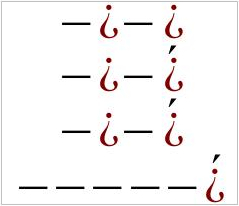
\includegraphics[width=20mm]{./imgs/fig1.jpg}
\caption{I}
\end{minipage}
 \hfill
\begin{minipage}{0,4\textwidth}
\centering
  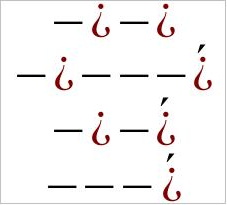
\includegraphics[width=20mm]{./imgs/fig2.jpg}
\caption{II}
\end{minipage}
\end{figure}

O terceiro verso, como dois trímetros (6 pés jâmbicos) e o quarto como
dois tetrâmetros (8 pés jâmbicos), com a respectiva tonicidade:

\begin{verse}
\emph{Nótch smótritsa, kak Tiútchev,} \\
Ночь смотрится, как тютчев, \\[8pt]
\emph{Zamiérnoebezmiérnympólnia.} \\
Замерное безмерным полня \\[8pt]
\end{verse}


\begin{figure}[!ht]
\begin{minipage}{0,4\textwidth}
\centering
  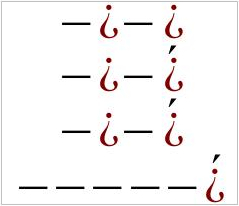
\includegraphics[width=20mm]{./imgs/fig1.jpg}
\caption{III}
\end{minipage}
 \hfill
\begin{minipage}{0,4\textwidth}
\centering
  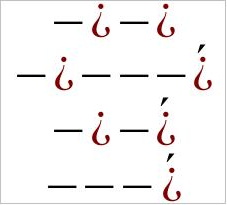
\includegraphics[width=20mm]{./imgs/fig2.jpg}
\caption{IV}
\end{minipage}
\end{figure}

Nessa quadra, vista como um todo, ligada pela rima \versal{ABAB} e pelo acento na
6ª sílaba de todos os versos, (o verso russo é sílabo"-tônico), é
possível notar a contraposição dos versos longos (ambos com acentos na
décima sílaba) e dos versos curtos, (ambos com acento na segunda
sílaba).

Vale a pena notar também a mobilidade dos acentos na sexta sílaba (no \versal{I}
verso, é o primeiro acento; no \versal{II} verso, é o segundo acento; no \versal{III}
verso, é o terceiro acento; no \versal{IV} verso, é o segundo acento). Tomando"-se
como eixo de simetria a sexta sílaba, verifica"-se que o \versal{II} e o \versal{IV} versos
ficam no centro; o \versal{I} é deslocado para a direita, o \versal{III} para a esquerda,
configurando uma construção em degraus.

O vocalismo da quadra revela propriedades surpreendentes (o
consonantismo é pouco relevante). A série \emph{e/o/u} constitui 70\% da
quantidade de vogais do poema: \emph{e} é acentuado três vezes, \emph{u}
três vezes e \emph{o} seis vezes.

Assim se distribuem essas vogais pelos versos (repare"-se a
especularidade de \versal{I} e \versal{III} e o paralelismo de \versal{III} e \versal{IV}): \\

o u u

o e o

o o u

e e o \\

Ainda mais surpreendente é observar a totalidade orgânica da estrutura
vocálica do poema e seu desenrolar"-se dinâmico (\emph{e} ocupa os três
pontos da linha superior, \emph{o} os seis pontos da linha central e
\emph{u} os três pontos da linha inferior do esquema):

\begin{figure}[!ht]
\centering
  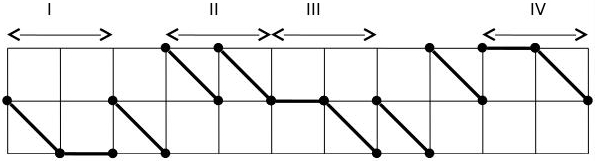
\includegraphics[width=95mm]{./imgs/fig5.jpg}
%\caption{III}
\end{figure}

Este esquema do movimento das vogais representa quase uma simetria
inversa plena, onde o centro é a primeira vogal do terceiro verso, ou
seja, \emph{o} da palavra \emph{nótch}, \emph{no qual cai o único
acento fora do esquema métrico do poema!}

Nessa palavra monossilábica se concentra toda a energia rítmica e
fonética do poema, o que é plenamente compreensível pois \emph{nótch}
(noite) é justamente seu centro imagético.

Ao mesmo tempo, o princípio tricotômico do poema é anunciado pelo \versal{I}
verso, em todos os níveis da estrutura: três acentos, trivocalismo,
trivocabular, o que prenuncia os três nomes do encantamento.

A palavra mitopoética baseia"-se na identidade artística entre o
microcosmo do poema, o cosmo da poesia e o macrocosmo da natureza.
Justamente por isso deve"-se ir além dos três nomes do encantamento. O
que dá continuidade à serie seria, por assim dizer, o nome dos nomes dos
nomes. Compreende"-se que este nome de ``terceira ordem'' só poderia
sugerir a saída para além dos limites desse mundo.

O acerto dessa hipótese confirma"-se pela história do texto da
``Encantação pelo nome''. Dela, com efeito, chegaram até nós quatro
variantes do último verso. A primeira é a que conhecemos; a segunda,
contém uma palavra com uma variação de \emph{ié} para \emph{í}, uma vez
que K. usou para o \emph{ie} da palavra \emph{bezm\emph{íe}rnym} a letra
russa \emph{iat} (o antigo \emph{ie} usado no eslavo"-eclesiástico),
colocando em cima dela um ponto. Esse fato permitiu que se lesse a
palavra como se em lugar de \emph{ie} estivesse a antiga letra
\emph{i}, ficando a palavra, portanto, \emph{bezmírnym}. Na terceira
variante temos \emph{zamírnym} em lugar de \emph{bezmírnym}.
Focalizando"-se o último verso nas três primeiras variantes, temos:

\begin{verse}
\versal{I}: \emph{Zamiérnoe bezmiérnym pólnia} \\
(Enchendo o comensurável com o \\
incomensurável) \\[8pt]

\versal{II}: \emph{Zamiérnoe bezmírnym pólnia} \\
(Enchendo o comensurável com o \\
sem"-mundo) \\[8pt]

\versal{III}: \emph{Bezmiérnoie zamírnym pólnia} \\
(Enchendo o incomensurável com o \\
além"-mundo)
\end{verse}

Com efeito, se o mundo terrestre (Dostoiévski) é mensurável, o mundo
solar (Púchkin) é comensurável e o mundo estelar (Tiútchev) é
incomensurável, então o próximo passo só pode ser a saída para o
além"-mundo (o mundo do além). A mudança da raiz -\emph{mer} para
-\emph{mir} indica justamente a passagem para essa outra dimensão. Se
Dostoiévski, Púchkin e Tiútchev são três estágios de luminescência, o
quarto estágio pode também ser a passagem para além do mundo visível,
para a sua parte interior, invisível, imaginada. Ou a mudança do nome
para o número.

A quarta e última variante apresenta uma curiosa plurivocidade.
Curiosamente, em russo palavra \emph{mir} pode significar, ao mesmo
tempo ``mundo'' ou ``paz''. Literalmente, \emph{bezmirnoie} é o adjetivo
neutro que significa ``sem paz'', mas que, poeticamente, mantém,
latente, o sentido de ``sem"-mundo''.

Se \emph{mir} indicava antes ``mundo'', ``esfera terrestre'' e
\emph{bezmir} ``sem mundo'', \emph{mir} surge agora com o sentido de
``paz'', contrapondo"-se a ``guerra'', ``sem paz'', ``caos'', ``ruina'',
etc. (\emph{bezmir}):

\begin{verse}
\versal{IV}: \emph{Zamírnoie bezmírnym pólnia} \\
(Enchendo o além"-mundo de guerra)
\end{verse}

Disso segue a continuação da série: mensurável \emph{(miérnoie});
comensurável (\emph{zamiérnoie)}; incomensurável \emph{(bezmiérnoie});
do além"-mundo \emph{(zamírnoie}); e sem"-paz/guerra (\emph{bezmírnoie}),
onde o novo degrau não indica nenhuma etapa de luminescência, mas sim
sua ausência, o obscurecimento, a ruina, o caos, que também, na visão de
K., entra a compor a ordem universal.

Cada variante do poema não muda as precedentes e o poema respira,
enchendo as encantações de conteúdos novos, a cada vez. A obra é finita,
todas as vezes, mas é também inacabada, passível de modificações. O
organismo artístico cresce, mas em todas as variantes continua ele
mesmo, em sua plenitude e unicidade.

A história do texto da encantação não acaba aqui. Num
\emph{tour"-de"-force} extremado, Dugánov ainda nos revela a passagem da
``encantação pelo nome'' para a ``linguagem estelar''. Mas isso fica
para um próximo encontro.

Se o artista Manoel de Barros mergulha no caos e mistura e remodela os
signos aviltados, encanta as palavras para que nos possam falar de novo
do sagrado e do mágico, numa tela que também é barro, que também é chão,
que também é volta às origens, o artista Velimir Khlébnikov, nesse mesmo
esforço de unir as pontas soltas da natureza e da cultura, produz
rigorosos desenhos, capazes de criar uma nova ordem no universo das
palavras reinventadas, onde o obscurecimento, o caos, a ruina e mesmo a
morte entram na mesma harmonia cósmica universal.

\chapter*{Aspectos da natureza em Velimir Khlébnikov e em Manoel de Barros}

\addcontentsline{toc}{chapter}{Aspectos da natureza em V. Khlébnikov e em M. de Barros}
\hedramarkboth{Aspectos da natureza em V. Khlébnikov e em M. de Barros}{}

Certamente o grande poeta brasileiro do Pantanal, Manoel de Barros
(1916--2014) é, entre os poetas contemporâneos, o que mais se parece
com o russo Velimir Khlébnikov, o ``mestre'' dos poetas cubofuturistas
russos, mesmo se --- após convergirem na re"-criação do mundo da natureza
de base sensorial --- eles se tenham se diferenciado em sua
transcendência.

\section{I. O Manifesto}

Entre os vários diálogos"-entrevistas que podem ser encontrados como
apêndices em um dos últimos livros de Manoel de Barros, \emph{Gramática
expositiva do chão}\endnote{*Texto apresentado em inglês, em junho de
  1994, na Universidade de Berkeley, durante o Congresso Internacional da \versal{IASS}.

\versal{BARROS}, Manuel. \emph{Gramática expositiva do chão (poesia quase
  toda)}. Rio de Janeiro: Civilização Brasileira, 1990.}, este trecho
pode ser lido como um manifesto:

\begin{quote}
Achava e acho ainda que não é hora de reconstrução. Sou mais apalavra a
ponto de entulho ou traste. (\ldots{}). Agora a nossa realidade se desmorona.
Despencam"-se deuses, valores, paredes\ldots{} Estamos entre ruinas. A nós,
poetas destes tempos, cabe falar dos morcegos que voam por dentro dessas
ruínas. Dos restos humanos fazendo discursos sozinhos nas ruas. A nós
poetas cabe falar do lixo sobrando e dos rios podres que correm por
dentro de nós e das casas. Aos poetas do futuro caberá a reconstrução ---
se houver reconstrução. Porém a nós, a nós, sem dúvida, resta falar
dos fragmentos, do homem fragmentado que, perdendo suas crenças, perdeu
sua unidade interior. É dever dos poetas de hoje falar de tudo que
sobrou das ruínas --- e está cego. (pp. 308, 309) (\ldots{}) Pegar certas
palavras já muito usadas, como as velhas prostitutas, decaídas, sujas de
sangue e esterco --- pegar essas palavras e arrumá"-las num poema, de
forma que adquiram nova virgindade. Salvá"-las, assim, assim, da morte
por clichê. Não tenho outro gosto maior do que descobrir para algumas
palavras relações dessuetas e até anômalas. (p. 308) Cego e torto e
nutrido de cinzas (\ldots{}) Só os poetas podem salvar o idioma da esclerose.
Além disso a poesia tem a função de pregar a prática da infância entre
os homens. (\ldots{}) Se a poesia desaparecer do mundo, os homens se
transformariam em monstros, máquinas, robôs. (p. 310). Um fundo amor
pelos humilhados e ofendidos de nossa sociedade, banha quase toda a
poesia de hoje. Esse vício de amar as coisas jogadas fora --- eis minha
competência (p. 311).
\end{quote}

No primeiro manifesto do Cubo"-futurismo ``Uma bofetada no senso comum'',
redigida por V. Maiakóvski, V. Khlébnikov, D. Burliuk, A. Krutchônikh e
publicado em Moscou em 1912, pode se ler:

\begin{quote}
\noindent{}Ordenamos que sejam considerados direitos dos poetas:

\noindent{}\versal{I} --- aumentar o volume do vocabulário por meio de palavras arbitrárias
ou derivadas (inovação através das palavras);

\noindent{}\versal{II} --- e se, até o presente momento, ainda permanecerem em nossos textos
as marcas sujas de seu ``bom senso'' e ``bom gosto'', já neles palpita,
pela primeira vez, os Trovões da Nova Recém"-chegada Beleza do Mundo que
carrega seu valor em si mesma e que gira em volta de si mesma.
\end{quote}

É assim que Khlébnikov desenvolve esses dois itens, numa série de
fragmentos escritos entre 1919--1920 e publicados em \emph{Nossa Base},
na revista \emph{Liren} (Kharkov, 1920):

\begin{quote}
Se você se encontrar no meio de uma floresta, você verá carvalhos,
pinheiros, bétulas\ldots{}

Toda essa variedade de folhagens, troncos, moitas é criada a partir de
um punhado de sementes que dificilmente podem se distinguir uma das
outras. A futura floresta está completamente contida na palma de sua
mão.

A ``criação de palavras'' (``verbocriação'') ensina que a inteira
variedade das palavras provém dos sons fundamentais do alfabeto que
substituem as sementes por palavras.

Esses pontos iniciais permitem a construção da língua e seu novo
semeador pode simplesmente encher a palma da sua mão com os 28 sons do
alfabeto, as sementes da língua. Se você dispuser de oxigênio e de
hidrogênio, poderá encher de água o fundo seco do mar e os braços vazios
dos rios.

A inteira plenitude da língua pode ser decomposta em unidades
fundamentais de ``verdades primárias''; poderá, então, elaborar para o
material sonoro uma espécie de tabela de Mendelêiev ou leis de Moseley,
a fase final do pensamento químico.
\end{quote}

Se Manoel de Barros diz ``somente os poetas podem salvar a língua da
esclerose\ldots{} e os governos mais sábios deveriam contratar os poetas para
isso''\endnote{\versal{BARROS}, Manuel. 1990, p. 310.}, assim escreve
Khlébnikov:

\begin{quote}
Os homens públicos nunca pensaram ao estrago que pode causar uma palavra
mal construída. Isso porque não existem livros que declarem o direito do
povo no que se refere à língua. Nem o direito dos engenheiros e
construtores de pontes e das estradas da língua. Muitas vezes o espírito
da língua toleraria uma palavra só, a simples permutação de um som
consonantal na palavra existente, mas --- em lugar disso --- todos usam um
circunlóquio, uma expressão descritiva que é completa e frágil. Quem, na
época do pensamento universal passaria de New York para ir de Moscou a
Kiev? Justamente, qual linha da língua livresca moderna está livre
dessas rotatórias? Nenhuma, pois não há nenhuma ciência da criação da
língua.

Se pudéssemos descobrir que as leis dos corpos simples do alfabeto são
semelhantes às de uma inteira família de línguas, poderíamos elaborar ---
para essa inteira família --- uma nova língua universal, um trem que
poderia partir de New York para Moscou, usando os espelhos das palavras.
Se dois vales aparecem separados por uma cadeia de montanhas, o viajante
que quer passar por eles pode tanto provocar a explosão dessas montanhas
como pode dar a volta delas e entrar em cada um dos vales. A
verbocriação é a explosão do silêncio linguístico, das camadas
surdo"-mudas da língua. A palavra é feita do puro e do habitual.

Poderia se pensar que a porção noturna estrelada e a porção diurna,
ensolarada, estão escondidas nelas.

Isso ocorre porque o significado comum de uma palavra encobre todos os
outros significados, da mesma forma que, quando surge o dia, a noite
estrelada e as estrelas desvanecem.

A palavra ``autônoma'' renuncia aos fantasmas de uma situação prática e
salienta, faz surgir, em lugar da mentira automática, o pôr"-do"-sol
estrelado.

Assim, a noite da vida corrente são os significados fracos das palavras,
que se parecem com as visões imprecisas da noite. Pode"-se dizer que a
língua prática é feita das sombras atiradas pelas grandes leis da
palavra pura, projetadas sobre uma superfície irregular.\endnote{\versal{KHLÉBNIKOV},
  Velimir. \emph{Le pieu du Futur}. Lousanne: Editions L'Age d'Home.
  1970.}
\end{quote}

A física moderna assimilou, de uma forma que nós não sabemos se
conveniente ou não, a linguagem poética. Ela propõe equações que se
utilizam de termos vagos, como o número quântico. ``O que o senhor poderia
dizer quanto a esta apropriação?'' --- foi perguntado, em uma entrevista, a
Manoel de Barros. Aqui está a sua resposta escrita:

\begin{quote}
Sei que urdir conotações dementes é saudável para a poesia. Agora eu não
sei se a quântica aceita isso sem atolar na pedra. (p. 318) As nossas
particularidades só podem ser universais se comandadas pela linguagem.
Subjugadas por um estilo. Acho, por fim, que jamais alcançaremos o veio
da criação. (p. 334) Como encontrar as funções todas de uma palavra?
Assim é o homem neste desolo. Nunca se vê completo. Há uma indigência
bugral\endnote{De acordo com Gilberto Freyre, em Casa Grande \&
  Senzala. Brasília: Ed. Universidade de Brasilía, 1963, p.178, ``A
  denominação de bugres dada pelos portugueses aos indígenas do Brasil
 em geral e a uma tribo de São Paulo em particular talvez exprimisse o
  horror teológico de cristãos mal saídos da Idade Média ao pecado
  nefando, por eles associado sempre ao grande, ao máximo, de
  incredulidade ou heresia. Já para os hebreus o termo \emph{gentio}
  implicava ideia de sodomita; para o cristão medieval foi o termo
  \emph{bugre} que ficou impregnado da mesma ideia pegajosa de pecado
  imundo. Quem fosse herege era logo havido por sodomita; como se uma
  danação arrastasse inevitavelmente à outra. \emph{``Indeed, so closely
  was sodomy assoaciated with heresy that the same name was
  applied to both''}, escreve Westermarck. E acrescenta: \emph{``the
  French \emph{bougre} (from the Latin \emph{Bulgarus}, \emph{Bulgarian}), as also its English
  synonim, was originally a name given to a sect of heretics who came from
  Bulgaria in the eleventh century, and was afterwards applied to other
  heretics, but at the same time it became the regular expression for
  a person guilty of unnatural intercourse''.}} em mim que só aguenta
espiar de cócoras. Sem agir. Não gosto de aprender novidades. Só gosto
de me repetir pra criar minha linguagem. Resta sempre uma verdez primal
em cada palavra. Cada palavra pode ser o germe de uma obscura
existência. (\ldots{}) Independente da verdade --- e até contra ela --- o do
que gosto mais é de fazer frase ao dente. Troco isso por verdades
científicas. E volto soma. Mistério tem mais camadas do que a ciência.
Os arcanos florescem. (p. 342) \endnote{\versal{BARROS}, 1990, pp. 318, 334,
  342.}
\end{quote}

E aqui está a resposta possível de Khlébnikov:

\begin{quote}
Pode"-se pensar que a ciência acompanha \emph{pari passu} a mesma estrada
percorrida pela língua. A lei universal de Lorentz diz que um corpo se
achata na direção transversal à pressão a que ele é submetido. Essa lei,
contudo, é --- ao mesmo tempo --- própria da matéria do ``elemento nome''.

Qualquer que venha a ser o sentido da letra ``л'', em todos os casos, o
raio da força do movimento expande"-se sobre uma superfície transversal
ao raio, até que esse raio de força possa atingir seu equilíbrio no jogo
das forças.

Quando o raio tiver percorrido a superfície transversal, o peso do raio
tornar"-se"-á leve e o raio não mais girará.

Por acaso qualquer língua está a par da oscilação transversal do raio?
Por acaso alguma língua sabe que \versal{R} se torna \versal{R}=$\sqrt{1-\frac{v^{2}}{cx^{2}}}$?
Onde ``v'' = velocidade do corpo e ``c'' = velocidade da luz? Como todas as
aparências levam a crer, a língua parece ser tão sabia quanto a
natureza, mas nós só aprenderemos a lê"-la quando impelidos pela ciência
e --- mais ainda --- apenas pelo impulso da ciência teremos o condão de
adivinhar a inteira sabedoria de uma língua, que é sábia justamente por
ser, ela mesma, parte da natureza. Às vezes ela nos ajuda a resolver
problemas abstratos. Assim, com a ajuda da língua, fazemos o esforço de
medir o comprimento das ondas do bem e do mal. A sabedoria da língua nos
mostra há muito tempo a natureza iluminada do mundo. O ``eu'' do mundo
coincide com a vida da lua. O fogo penetra pelos hábitos. O homem vive
neste mundo cuja velocidade limite é de 300.000 Km, mas alguma vez pensa
ele num outro mundo com uma velocidade que excede de muito a velocidade
da luz? A sabedoria da língua precedeu a sabedoria de todos as
ciências.\endnote{\versal{KHLÉBNIKOV}, Velimir. \emph{Le pieu du futur}.
  Lousanne: Éditions L'Age d'Homme. 1970, p. 47}
\end{quote}

\section{II. As personagens}

Assim se descreve Manoel de Barros:

\begin{quote}
O que escrevo resulta de meus armazenamentos ancestrais e de meus
envolvimentos com a vida. Sou filho e neto de bugres andarejos
portugueses melancólicos. Minha infância levei com árvores e bichos do
chão. Essa mistura jogada depois na grande cidade deu borá: um mel sujo
e amargo. Se alguma palavra minha não brotar desse substrato, morrerá
seca. (p. 315) Quando de primeiro o homem era só, Bernardo era. Veio de
longe com a sua pré"-história. Resíduos de um Cuiabá"-garimpo, com vielas
rampadas e crianças papudas, assistiram seu nascimento.

Agora faz rastros neste terreiro. Repositório de chuva e
bosta de ave é seu chapéu. Sementes de capim, algumas, abrem"-se de suas
unhas, onde o bicho de porco entrou cresceu e já voou de asa e
ferramentas.

De dentro de seus cabelos, onde guarda seu fumo, seus cacos de vidro,
seus espelhinhos --- nascem pregos primaveris.

Não sabe se as vestes apodrecem no corpo senão quando elas apodrecem.

E muito apoderado pelo chão esse Bernardo. Seu instinto e seu faro
animal vão na frente. No centro do escuro se espraiam. Foi resolvida em
língua de folha e de escama, sua voz quase inaudível. E que tem uma
caverna de pássaros dentro de sua garganta escura e abortada.

Com bichos de escama conversa. Ouve de longe a botação de um ovo de
jacaroa. Sonda com olho gordo de hulha quando o sáurio amolece a oveira.
Escuta o ente germinar ali ainda implume dentro do ventre. Os embriões
do ovo ele vislumbra prazenteiro. Ri como fumaça. Seu maior infinito!
Quando o corpo do sáurio se espicha no areão, a fim de delivrar"-se,
Bernardo se ilumina. Pequena luzerna no pavio de seu olho brandeia. A
jacaroa e ele se miram imaculados. A própria ovura! Passarinhos do mato
bentevi joão"-ferreira sentam no ombro desse bandarra para catar
imundícia orvalho insetos. Só dá de banda. Nos fundos da cozinha onde se
jogam latas de vermes ávidos, lesma e ele se comprazem. Teias o
alcançam. Lagartas recortam seu dólmã verdoso. Formigas fazem"-lhe
estradas\ldots{} Unge com olho as formigas. No pátio cachorro acua ele.
(Pessoas com ar de quelônio cachorro descompreende.) Galinhas bicoram
seu casco. Mal desenxerga. (Nem mosca nem pedrada desviam ele de ser
obscuro.) Bernardo está pronto a poema. Passa um rio gorjeado por perto.
Com as mãos aplaina as águas. Deus abrange ele.\endnote{\versal{BARROS}, 2010,
  p. 243, 244, 315.}
\end{quote}

E agora, ouçamos Khlébnikov:

\begin{quote}
``O homem sábio do ano de 2222 deu"-me a tarefa de compor descrições do
homem''

Eu preenchi todas as questões e apresentei, eu relatório.

Número de olhos -- dois

Número de braços -- dois

Número de pernas -- duas

Número de dedos -- vinte.\endnote{\versal{KHLÉBNIKOV}, Velimir. In: \emph{Apud}
  Dugánov, \versal{R. V.} \emph{Velimir Khlébnikov -- Priróda Tvórtchestvo}. (Р.
  В. Дугaнов. \emph{Велимир Хлебников}. \emph{Природа творчества}.
  [\emph{Velimir Khlébnikov. A natureza da criação}]) Moskvá,
  Soviétski Pissátel', 1990, p. 27.}
  \end{quote}



\begin{quote}
Nós discutimos quanto às vantagens e as desvantagens desses números, ``É
possível que esses números mudem, às vezes?\ldots{}'' Eles são números
limites, eu respondi. --- O fato é que às vezes se encontram pessoas com
um braço ou uma perna. O número dessas pessoas costuma aumentar
sensivelmente cada 317 anos. Mas isso é suficiente --- ele disse --- para
compor a equação da morte. A língua --- observou o sábio do ano de 2222 ---,
é a eterna primavera do conhecimento. De que forma se relacionam entre
si o tempo e a gravitação? Não há dúvida que o tempo está para o demo.
Mas é possível endemoniar"-se sob um peso pesado? Não, o peso absorve as
forças do demo. E onde está um, não está o outro. Em outras palavras, o
tempo absorve as forças do peso mas não irá desaparecer o peso lá onde
está o tempo? De acordo com o espírito de sua língua, o tempo e o peso
são duas diferentes observações de uma única e mesma força.\endnote{\versal{KHLÉBNIKOV},
  Velimir. In: \emph{Apud} Dugánov, R. V. \emph{Velimir Khlébnikov --
  Priróda Tvórtchestvo}. (Р. В. Дуганов. \emph{Велимир
  Хлебников}. \emph{Природа творчества}. [\emph{Velimir Khlébnikov. A
  natureza da criação}]) Moskvá, Soviétski Pissátel', 1990, p.29. (Note-se que, em russo \emph{demônio} e \emph{peso} têm pronúncia
  parecida: respectivamente \emph{biés} e \emph{viés}.)}
\end{quote}

\section{III. A leitura}

Manoel de Barros:

\begin{quote}
A única palavra citadina legítima que consta de meus arquissemas é
\emph{parede}. (\ldots{}) As outras dez ou doze palavras que são meus
arquissemas, vêm de minha infância. São elas árvores: sapo, lesma,
antro, musgo, boca, rã, pedra, caracol. Acho que são as palavras que me
comandam subterraneamente. Arquissemas, aprendi de um filólogo, (\ldots{}) são
palavras logradas dos nossos armazenamentos ancestrais, e, que ao fim
norteiam o sentido de nossa escrita.\endnote{\versal{BARROS}, 2010, p. 331.}
\emph{Me parece} que \emph{olhando} pelos cacos, pelos destroços, pela
escória \emph{eu estaria} tentando juntar fragmentos de mim mesmo
espalhados por aí --- \emph{Estaria} me dando a unidade perdida. E
que \emph{obtendo a redenção das pobres coisas, eu estaria obtendo a
minha redenção}. (Só os fragmentos me unem?)\endnote{\versal{BARROS}, 2010, p.
  328.}
\end{quote}

Se começarmos a analisar as recorrências lexicais nas obras de
Khlébnikov, descobriremos que o ``olho'' muitas vezes está no lugar da
``boca'' de Manoel de barros; quanto a água, pedra, noite, morte,
gafanhoto, céu, elas coincidem nos dois poetas, com outras variantes do
mundo vegetal e mineral. Afora palavras como ``urso'' e ``cisne'' que,
obviamente, pertencem ao ``reservatório ancestral'' de Khlébnikov e não
ao de Barros, outras que não encontraremos nos arquissemas do brasileiro
são as palavras ``rosto'', ``semblante'', um dos motivos mais frequentes
nos poemas de Khlébnikov:

\begin{verse}
Bobeóbi cantar de lábios,\\
Lheeómi cantar de olhos,\\
Cieeo cantar de cílios,\\
Stioeei cantar do rosto\\
Gri"-gsi"-gseo o grilhão cantante.\\
Assim no bastidor dessas correspondências\\
Transespaço vivia o semblante.\endnote{\versal{CAMPOS}, Augusto
  e Haroldo e \versal{SCHNAIDERMAN}, Boris (org. e trad.). \emph{Poesia Russa
  Moderna}. São Paulo: Brasiliense, 1985, p. 84. (Este poema foi
  traduzido por Haroldo de Campos).}
\end{verse}

A unidade dos fragmentos, que, em Manoel de Barros, curiosamente, é
obtida através dos significados em História Natural:

\begin{verse}
\emph{Lesmas, s.f.}\\
Semente molhada de caracol que se arrasta \\
sobre as pedras, deixando um caminho \\
de gosma escrito com o corpo \\
Indivíduo que experimenta a lascívia do \\
ínfimo \\
Aquele que viça de líquenes no jardim\endnote{\versal{BARROS}, 2010, p. 215.}
\end{verse}

em Khlébnikov é conseguida através da História da Humanidade que ele
tenta descobrir, olhando"-a cosmicamente:

\begin{verse}
Tempos juncos \\
À margem do lago. \\
Onde as pedras são tempo \\
E o tempo é de pedra. \\
No lago da margem \\
Tempos, juncos, \\
Na margem do lago, \\
Santos, juntos.\endnote{\versal{KHLÉBNIKOV}, Velimir. In: Dugánov, R. V.
  \emph{Velimir Khlébnikov -- Priróda Tvértchestvo}. (Р. В. Дуганов.
  \emph{Велимир Хлебников}. \emph{Природа творчества}. [\emph{Velimir
  Khlébnikov. A natureza da criação}]) Moskvá, Soviétski Pissátel',
  1990. p. 40. E em \emph{Poesia Russa Moderna}, \emph{op. cit}. p, 78, na
  tradução de Augusto de Campos e Boris Schnaiderman.}
\end{verse}

Quando os fragmentos se aglutinam, em Manoel de Barros, eles florescem
liricamente numa espécie de apoteose dos sentidos,

\begin{verse}
No chão, entre raízes de inseto, esma e cisca \qb{}o sabiá. \\
É um sabiá de terreiro. \\
Até junto de casa, nos podres dos baldrames, \\
vem apanhar grilos gordos. \\
No remexer do cisco adquire experiência de \qb{}restolho. \\
Tem uma dimensão além de pássaro, ele! \\
Talvez um desvio de poeta na voz. \\
Influi na doçura de seu canto o gosto que \\
pratica de ser uma pequena coisa \qb{}infinita do chão. \\
Nas fendas do insignificante ele procura \qb{}grãos de sol. \\
A essa vida em larvas lateja debaixo das \\
árvores o sabiá se entrega. \\
Aqui desabrocham corolas de jias! \\
Aqui apodrecem os vôos. \\
Sua pequena voz se umedece de ínfimos \qb{}adornos. \\
Seu canto é o próprio sol tocado na flauta! \\
Serve de encosto pros corgos. \\
Do barranco uma rã lhe entarda os olhos. \\
Esse ente constrói o álacre. \\
É intenso gárrulo: como quem visse a aba \qb{}verde das horas. \\
É ínvio o ardente que o sabiá não diz. \\
E tem espessura de amor.\endnote{\versal{BARROS}, 2010, p.211-212}
\end{verse}

Em Khlébnikov, a organização dos fragmentos está acima e além
florescência. Cada mínimo poema tem ``seu próprio Deus, sua própria
crença, seu próprio código'':

\begin{verse}
Quando morrem os cavalos -- respiram, \\
Quando morrem as ervas -- secam, \\
Quando morrem os sóis -- se apagam, \\
Quando morrem os homens -- cantam.\endnote{\versal{KHLÉBNIKOV}, Velimir.
  In: Duganov, R. V. \emph{Velimir Khlébnikov -- Priróda Tvórtchestvo}.
  (Р. В. Дуганов. \emph{Велимир Хлебников}. \emph{Природа творчества}.
  [\emph{Velimir Khlébnikov. A natureza da criação}]) Moskvá,
  Soviétski Pissátel', 1990, p.6. (Tradução nossa).}
\end{verse}

E em cada um de seus poemas a vida é ``a necessária e regulada
integração de elementos primários.''\endnote{\versal{KHLÉBNIKOV}, Velimir. In:
  Dugánov, R. V. \emph{Velimir Khlébnikov -- Priróda Tvórtchestvo}. (Р.
  В. Дуганов. \emph{Велимир Хлебников}. \emph{Природа творчества}.
  [\emph{Velimir Khlébnikov. A natureza da criação}]) Moskvá,
  Soviétski Pissátel', 1990, p.20.}

O que pode haver de mais elementar do que esses terra, água, fogo e ar,
tomados como símbolos da geração de nosso universo e dos seres que nele
andam, rastejam, trepam ou voam? Nesse começo mítico e poético ambos os
poetas coincidem. Barros, vendo o homem no \emph{clinamen} dos
diferentes reinos:

\begin{verse}
\emph{Inseto, s.m.} \\
Indivíduo com propensão a escória \\
Pessoa que se adquire da umidade \\
Barata pela qual alguém se vê \\
Quem habita os próprios desvãos \\
Aqueles a quem Deus gratificou com a \qb{}sensualidade (\ldots{})\endnote{\versal{BARROS},
  2010, p. 216.}
\end{verse}

E Khlébnikov, vendo a natureza no homem e através do homem:

\begin{verse}
Neste dia de ursos cerúleos \\
A correr sobre cílios tranquilos \\
Transvejo para além da água azul \\
O acordar na taça das pupilas. \\[8pt]
Na colher de prata de olhos latos \\
Vejo a procelária em mar sonoro \\
E ao largo vai a Rússia dos pássaros \\
Transvoando entrecílios ignotos. \\[8pt]
Marventoso em celamor soçobra \\
A vela de alguém na azul esfera, \\
E eis que o desesoero tudo engolfa \\
Trovão e porvir da primavera\endnote{Nova Antologia \emph{POESIA RUSSA
  MODERNA}, p.93 (Trad. de Haroldo de Campos e Boris Schnaiderman)}
\end{verse}

Depois, contudo, essa mesma natureza, uma vez animada e humanizada,
tornou"-se berço e túmulo dos resíduos da vida e das personagens
históricas. Em ``Escuridades vermelhas'', de Barros, lemos:

\begin{verse}
O veneno ingerido pela mosca deixa \\
A curta raiz de sua existência \\
Exposta às vermelhas trevas.
\end{verse}

E:

\begin{verse}
Contou que achara a mulher dentro de um \qb{}pote e a bebeu. \\
Sem amor é que encontramos com Deus -- \qb{}me diz \\
O mundo não é perfeito como um cavalo -- \qb{}me diz. \\
Vê trinos de água nos relógios. \\
E para moscas bate continência. \\
Eu volto de sarjeta para casa.\endnote{\versal{BARROS}, 2010, p. 221.}
\end{verse}

Tal como em Khlébnikov, até o momento em que, dialeticamente, eventos
históricos tornam"-se princípios primevos, inelutáveis fenômenos da
natureza:

\begin{verse}
Herdades noturnas, gengiscantem! \\
Crepitai, bétulas azuis! \\
Albas da noite, zaraturvem \\
Ao céu cerúleo mozarteante! \\
Goyam trevas como nuvens! \\
Roops é um cirro soturno! \\
Voa uma tromba de risos, \\
Enfrento firme o verdugo, \\
Gargalham garras de gritos, \\
E em torno o silêncio escuro. \\
A mim convoco os valentes \\
Saem dos rios os afogados, \\
O miosótis estridente, \\
Declama a velames pardos. \\
Gira o eixo cotidiano, \\
Move"-se a massa vespertina, \\
Nas águas da noite vogando \\
(Sonho) uma carpa"-menina. \\
Mamáj -- pinhos ao vento! \\
Nuvens nômades do Báti! \\
Como cains do silêncio \\
Palavras santas me abatem. \\
Passo tardo, cercado de tropas, \\
Asdrúbal azul vai ao baile das tochas.\endnote{Nova Antologia
  \emph{POESIA RUSSA MODERNA}, p.91 (Trad. de Haroldo de Campos)}
  \end{verse}

Neste exato momento de síntese e clímax, quando, em Khlébnikov, as
camadas míticas exigem a intervenção, o ``cantar'' do homem, a conversão
do finito ao infinito:

\begin{verse}
Os deuses, quando amam \\
Condensam em medida o espanto da esfera \\
Com Púchkin a chama do amor pela \qb{}camareira de Volkónski\endnote{\versal{KHLÉBNIKOV},
  Velimir. In: Dugánov, R. V. \emph{Velimir Khlébnikov -- Priróda
  Tvórtchestvo}. (Р. В. Дуганов. \emph{Велимир Хлебников}. \emph{Природа
  творчества}. [\emph{Velimir Khlébnikov. A natureza da criação}])
  Moskvá, Soviétski Pissátel', 1990, p.9.(Tradução nossa).}
\end{verse}

em Manuel de Barros, o bugre se desnomeia:

\begin{verse}
O homem de lata \\
é uma condição de lata \\
e morre de lata \\[8pt]
O homem de lata \\
é um passarinho \\
de viseira \\
não gorjeia \\[8pt]
Caído na beira \\
do mar \\
é um tronco rugoso \\
e cria limo \\
na boca\endnote{\versal{BARROS}, 2010, pp. 160-161.}
\end{verse}

Na grande comoção de seu século, na História de que foi testemunha
ativa, Khlébnikov --- o poeta --- propôs"-se a captar a profunda essência
particular de sua palavra como transcendência para o universal.

Das profundezas da região lodosa do Pantanal, a palavra do poema Manoel
de Barros transubstancia a natureza e desnomeia seus herois. O bugre não
quer a realidade corrompida de nosso tempo e lugar, nem deseja ou pode
sua palavra encontrar a si mesma no epos.

\section{BIBLIOGRAFIA}

\versal{BARROS}, Manuel. \emph{Gramática expositiva do chão (poesia quase toda)}.
Rio de Janeiro: Civilização Brasileira, 1990.

\versal{CAMPOS}, Augusto e Haroldo de; \versal{SCHNAIDERMAN}, Boris (org. e trad.).
\emph{Poesia Russa Moderna}. São Paulo: Brasiliense, 1985.

\versal{DUGÁNOV}, R. V. \emph{Velimir Khlébnikov -- Priróda Tvórtchestvo}. (\versal{Р. В.}
ДУГАНОВ. \emph{Велимир Хлебников}. \emph{Природа творчества}.
[\emph{Velimir Khlébnikov. A natureza da criação}]) Moskvá,
Sovietski Pissátel', 1990.

\versal{FREYRE}, Gilberto. \emph{Casa Grande \& Senzala}. Brasília: Ed.
Universidade de Brasilía, 1963.

\versal{KHLÉBNIKOV}, Velimir. \emph{Le pieu du Futur}. Lousanne: Éditions L'Age
d'Hommme. 1970.

\chapter{Marina Tsvetáieva, poetisa russa: esboço de vida e
obra}


Nosso interesse por Marina Tsvetáieva data de 1968, quando saíram
publicados alguns de seus poemas pela primeira vez, no Brasil, em
\emph{Poesia russa moderna}\endnote{\versal{SCHNAIDERMAN}, Boris; \versal{CAMPOS},
  Haroldo de; \versal{CAMPOS}, Augusto de (org. e trad.) \emph{Poesia Russa Moderna}.
  Editora Civilização Brasileira. Rio de Janeiro, 1968. Na obra de Mario
  de Andrade \emph{A escrava que não é Isaura} (São Paulo, Tipologia
  paulista, 1925, p. 43) encontra"-se uma alusão à poetisa e à tradução
  de um de seus versos apenas: ``Épocas há em que o Sol é um pecado
  mortal''.} na tradução magistral de Haroldo e Augusto de Campos e
Boris Schnaiderman.

Estávamos, naquela época, entretidos com o estudo de Maiakóvski,
preocupados em captar a ``verdade'' de sua poesia (não mistificada,
pelas controvérsias dos críticos), querer descobrir sob a colorida capa
do Cubo"-futurismo as características estáveis de seu ``fazer'' mais
autêntico.

A penumbra de impressões conflitantes que embotava nossa percepção
dissipou"-se por completo ao ler o brilhante e certeiro poema que
Tsvetáieva lhe dedicou. Ei"-lo, como o lemos primeiramente, traduzido por
Haroldo de Campos:

\begin{verse}
Acima das cruzes e dos topos, \\
Arcanjo sólido, passo firme, \\
Batizado a fumaça e a fogo -- \\
Salve pelos séculos, Vladímir! \\[8pt]
Ele é dois: a lei e a exceção, \\
Ele dois: cavalo e cavaleiro. \\
Toma fôlego, cospe nas mãos: \\
Resiste, triunfo carreteiro. \\[8pt]
Escura altivez, soberba tosca, \\
Tribuno dos prodígios da praça, \\
Que trocou pela pedra mais fosca \\
O diamante lavrado e sem jaça. \\[8pt]
Saúdo-te, trovão pedregoso! \\
Boceja, cumprimenta -- e ligeiro \\
Toma o timão, rema no teu voo \\
Áspero de arcanjo carreteiro. 
\begin{flushright}
16 set. 1921\endnote{\versal{TSVETÁIEVA}, M. em \emph{Poesia Russa Moderna}, (trad. De Haroldo de Campos) op. cit. p.158.}
\end{flushright}
\end{verse}

A artista, que em poucos versos vigorosos conseguia colher a essência da
aparente contradição maiakovskiana (a lei e a exceção --- o cavalo e o
cavaleiro --- o bocejo e o cumprimento, etc.), caracterizá"-la e
resolvê"-la naturalmente, estava realizando da forma mais perfeita aquele
jogo dialético no qual Hegel\endnote{\versal{HEGEL,} Georg Wilhelm
  Friedrich. \emph{Esthétique -- ``La poésie''}. Paris: Aubier
  Montaigne, 1965.} quis justamente ver o cerne de toda Poesia.

A surpresa e o entusiasmo levaram"-nos a procurar as obras da poetisa e a
ver ultrapassadas, de longe, nossas expectativas.

Aconteceu conosco o que, como já constatou Cesare Pavese\endnote{\versal{PAVESE},
  Cesar. \emph{Il mestiere di vivere}. Torino: Einaudi, 1974, p. 171.},
costuma acontecer no mundo da literatura: a procura de uma coisa leva à
descoberta de outras (no nosso caso a procura de um poeta levou à
descoberta de dois\ldots{})

Foi assim que nos certificamos de quanto Marina Tsvetáieva era
desconhecida. Não apenas no mundo ocidental: além da \emph{Poesia russa
moderna}, à qual nos referimos, existia, editada pela Gallimard, uma
coletânea de poemas seus traduzidos por Elsa Triolet\endnote{\versal{TSVETÁIEVA},
  Marina. \emph{Poémes}. Trad. Elsa Triolet). Paris, 1968.}, um volume
de sua prosa, com a introdução de F. Stepun, editado em New
York\endnote{\versal{TSVETAIEVA}, M. \emph{Prosa}. New York, Chekhov Publish
  House, 1953.}, e o estudo sobre sua vida e sua arte de S.
Karlinsky\endnote{\emph{Marina Cvetaeva - Her life and art}. Berkeley.
  Los Angeles, 1966.}, mas ela era desconhecida também no próprio mundo
soviético. Lá, a única obra que nos foi acessível foi uma seleção de
seus poemas, de certa forma parcial, precedida por uma introdução de V.
Orlóv\endnote{\versal{TSVETAIEVA}, M. \emph{Izbrannoie} (obras escolhidas).
  Moscou: Editora Estatal de Obras Literárias, 1961.}.

Todas as obras da poetisa (ou sobre ela), que consultamos em nosso
trabalho, foram publicados postumamente.

As referências que se encontram agora cada vez mais numerosas a seu
respeito\endnote{Cf. \versal{LOTMAN}, I. M. \emph{Struktura khuddjestvennovo
  tieksta} (Estrutura do texto artístico), Moscou: Editora (Arte), 1970.}
são apenas um indício de que, como queria Pasternak, está sendo
redescoberta. Ou simplesmente descoberta.

Em Moscou seus escritos se negociam no mercado negro, em Munique se
editam luxuosamente suas \emph{Obras Não"-reunidas}\endnote{Fink Verlag,
  München, 1971}, em Londres, Elaine Feinstein a traduz
entusiasticamente para o inglês, numa edição popular da \emph{Penguin
Modern European Poets}\endnote{\emph{Marina Tsvetayeva - Selected
  Poems} (traduzidos par Elaine Feinstein), Harmondsworth, Middlesex,
  1974}, em cuja introdução apoteótica Max Hayward a re"-situa, fazendo
suas as palavras de A. Akhmátova, ao lado dos três grandes últimos
poetas russos: Pasternak, Akhmátova e Mandelstam. Isso apenas para citar
as edições mais recentes, na época desse meu apanhado\endnote{Das obras que consultamos, \emph{Prosa
  e Stikhotvarienia} (Versos) foram publicados pela Bradda Books
  (Letchwarth, 1969) e \emph{Lebedini Stan'} (Acampamento de cisnes) e
  \emph{Marina Tsvetaeva - Stikhi, teatr, prosa} pela Ynca"-Press (Paris,
  respectivamente 1971 e 1976).}.

O impulso que nos levou a torná"-la centro de nosso estudo, e com isso,
talvez, mais conhecida em nosso meio, foi o mesmo que fez com que Elaine
Feinstein a traduzisse para o inglês:

\begin{quote}
\emph{Very soon I become obsessed with the sense that there was nothing
like Tsvetaieva in English. It was not only the violence of her
emotions, or the ferocity of her expression, I was overcome with
admiration for the extraordinary wholeness of her
self"-exposure}\endnote{Na introdução a \emph{Marina} \emph{Tsyetayeva --
  Selected Poems}, op. cit.}\emph{.}
\end{quote}

Se o que ela escrevia e a maneira pela qual o expressava eram tão
insólitos e tão inadequados para o seu mundo e para seu tempo que serão
justamente estas características a torná"-la mais valiosa para nossa
época.

Tal como aconteceu com John Donne tantos anos antes\endnote{Cf. \versal{DONNE},
  J. \emph{Selected Poems}. London - Melbourne -- Toronto: Heinemann,
  1961.}, só mais tarde terá sido descoberta a inteligência
(\emph{smartness}) apaixonada de suas imagens e devidamente apreciada a
deliberada aspereza e a angulosidade de seu estilo.

Refazer o caminho da formação de Marina Tsvetáieva é tarefa
particularmente difícil. Em primeiro lugar, por se tratar de uma poetisa
sempre ``inspirada'', quase sempre ``possessa''.

Em sua obra são mais importantes os ``motivos'' de inspiração do que
qualquer influência possível de outros autores. Ou, digamos assim, as
obras e as figuras dos outros autores são para ela motivos de inspiração
(Cf. Púchkin, Blok, Mandelstam, Shakespeare, Akhmátova, Maiakóvski,
Pasternak, as mitologias, as tragédias gregas, o folclore russo\ldots{}).
Mesmo quando ela aponta certas fontes (E. Rostand, V. Hugo, Rilke,
Napoleão), estão sempre sujeitas a sua elaboração poética, ou como ela
quer --- a seu olho interior.

São essa atemporalidade, essa nivelação contínua de fatos, coisas e
nomes, essa fusão do grande e do pequeno, ao calor do fogo de sua
percepção extraordinária, que dão a medida de sua inspiração:

\begin{verse}
O que aos outros não é preciso -- tragam \qb{}para mim! \\
Tudo há de queimar em meu fogo! \\
Atraio a vida, atraio a morte, \\
No leve regalo de meu fogo. \\[8pt]
A chama gosta de substâncias leves: \\
Ramos secos -- grinaldas -- palavras. \\
A chama arde desse alimento! \\
Levante-se, pois, mais puro que a cinza! \\[8pt]
Ave -- Fênix -- só no fogo eu canto! \\
Elevem para o alto minha vida! \\
Eu queimo alto -- e queimo até o fim! \\
E a noite, assim lhes será clara! \\[8pt]
Fogueira de gelo, fonte de fogo! \\
Levanto para o alto meu talhe elevado, \\
Levanto para o alto minha alta estirpe \\
De Herdeira e Conjurada!\endnote{De agora em diante, as traduções são
  de nossa autoria.}
\begin{flushright}
2 de setembro de 1918.
\end{flushright}
\end{verse}

Em seus termos: é a vida, é a morte, são as substâncias leves, elementos
de seu mundo poético, e o fogo --- a paixão com que os trata:

\begin{verse}
Negra como pupila, como pupila sugando a \\
Luz -- amo-te, noite aguçada. \\[8pt]
Dá"-me voz para cantar-te, ó promatre \\
Das canções, em cuja palma está a brisa \qb{}dos quatro ventos. \\[8pt]
Chamando-te, glorificando-te, sou apenas \\
Uma concha, onde ainda não calou o oceano. \\[8pt]
Noite! Eu gastei meus olhos nas pupilas \qb{}do Homem! \\
Incinera-me, negro sol-noite!
\begin{flushright}
9 de agosto de 1916.
\end{flushright}

Dois sóis congelam, tende piedade, \qb{}ó Deus! -- \\
Um no teu céu, outro no peito meu. \\[8pt]
Como esses sóis -- Algum dia terei cura? -- \\
Como esses sóis levam-me à loucura! \\[8pt]
E ambos congelam e seu raio não dói! \\
E o que gela primeiro é o mais quente \qb{}dos dois.
\begin{flushright}
5 de outubro de 1915.
\end{flushright}
\end{verse}

Por outro lado, a época que a poetisa viveu dificulta"-nos muito a
reconstituição desse mundo.

Dela sabemos ter nascido em Moscou, em 9 de outubro de 1892 (ou em 26 de
setembro como ela quer, pelo calendário antigo). Era filha de um
professor da Universidade de Moscou, colecionador e filólogo. A mãe,
musicista e poetisa apaixonada, inspirou"-lhe o amor à poesia e à
natureza. O pai, diz ela, ao trabalho.

Naturalmente, como seria de se esperar, a poesia leva"-a logo a conhecer
e amar todas os grandes poetas. Os russos e os alemães, em primeiro
lugar. Blok (``a melhor Rússia'') e Rilke (``a melhor Alemanha''). Entre
os russos, fora os já citados, Blok tem importância particular em sua
obra, no que se refere à ambiência de sua primeira fase, e Derjávin na
estruturação métrica de seus poemas líricos"-épicos mais complexos.

\begin{verse}
\emph{A Blok} \\[8pt]
Na mão -- um pássaro que cala, \\
Teu nome -- pedra de gelo na fala \\
Um movimento de lábios só. \\[8pt]
Teu nome -- cinco sons.\endnote{Anteriormente a reforma ortográfica, o
  nome ``Blok'' escrevia"-se com o assim chamado 'sinal duro' no final da
  palavra, tendo, portanto, cinco letras} \\
Uma bola em voo apanhada, \\
Um guizo na boca de prata. \\
Um seixo atirado num lago calmo, \\
Soam assim, como te clamo. \\
Ao leve tropel do casco noturno \\
Alto teu nome responde. \\
E o gatilho a estalar noturno \\
Lembra"-o, em nossa fonte. \\[8pt]
Teu nome -- ah, não consigo! \\
Teu nome -- um beijo no ouvido. \\
No gelo morno de pálpebras rígidas \\
Da neve é a beijo no mundo, \\
É um golpe de fonte, azul e frígido. \\
Em teu nome, o sono é profundo. 
\begin{flushright}
15 de abril de 1916
\end{flushright}
\end{verse}

Suas descobertas e afinidades vieram de acordo com seu amadurecimento
natural. Depois dos românticos franceses, além dos já citados:
Lamartine, Romain Roland, Vigny, descobre os realistas --- Proust, em
particular. Depois dos românticos ingleses (Byron, Shelley, Tennyson),
fixa"-se nos clássicos --- Shakespeare, fundamentalmente.

Difícil falar"-se em influência ou em coincidências. Em toda a sua obra
em prosa ou em verso há diálogos e transmutações com poetas e escritores
de todas as épocas e de todas as partes. Entretanto, no domínio
universal da poesia, em sua essência e sua expressão, ela é Marina
Tsvetáieva, única e incomparável.

\begin{verse}
Do tiro e quebranto, \\
Da toca e da prenda, \\
Divina Ichtar, \\
Resguarda"-me a tenda: \\[8pt]
Irmãos e irmãs. \\
Breu do meu metal, \\
Tina do meu mal, \\
Divina Ichtar, \\
Protege o carcás\ldots{} \\[8pt]
(Pegou"-me a cã!) \\[8pt]
Que o velho não aguente, \\
Que morra o doente, \\
Divina Ichtar, \\
Meu fogo resguarde\ldots{} \\[8pt]
(A chama arde!) \\[8pt]
Que o velho não dure, \\
Que o balde não ature, \\
Divina Ichtar, \\
Resguarde meu caldo\ldots{} \\[8pt]
(De peixes e auroras!) \\[8pt]
Pro velho ser mudo, \\
Pro jovem ser muda, \\
Divina Ichtar, \\
Sele meu muar \\
Na muda de luar!
\begin{flushright}
1923
\end{flushright}
\end{verse}

Parece paradoxal que um espírito apaixonado como o dela, que com dez
anos a faz escrever versos revolucionários, não a leve a se apaixonar
também por outra revolução, a de 17.

A explicação é uma questão de fatalidade e de fidelidade. Fatalidade,
porque em 1917, Marina já não mais era criança, nem adolescente. Mulher
feita, esposa de um oficial do exército Branco. Amadurecera cedo, em seu
entusiasmo absorvera avidamente e se saciara de impressões de um mundo
diferente.

A fidelidade a seus valores, a força de sua lembrança (``Quando se ama
alguém sempre se quer que ele vá embora, para poder melhor lembrá"-lo.
Quanto mais longe, mais longamente'') lhe dificultam o acesso a essa
Revolução. E quando a conhece, o que encontra já não é mais o momento
glorioso e idealista do risco e da conspiração, ao qual, sem dúvida, ela
aderiria.

Já não é nem mais a rápida fase revolucionária: é o período caótico e
arbitrário de pós"-revolução, onde num processo violento de nivelação,
muitos abusos, \emph{helás}, são inevitáveis.

O subjetivismo --- tudo nela é envolvimento pessoal ---, o alto apreço
(``Elevo para o alto meu alto valor\ldots{}'') em que Marina Tsvetáieva se
tem, impedem"-na de aceitar essa inevitabilidade. O preço da igualdade
para ela, que se considera muito acima, é caro demais.

As criaturas desse período, o arrivismo, o nepotismo, o abuso, o
provincianismo às quais ela se vê atirada, sufocam"-na:

\begin{verse}
Se a alma nasceu alada, \\
Cabanas ou palácios não são nada! \\
Gengis \emph{Cã} ---, a Horda, o que são no fundo? \\[8pt]
Meus, há dois inimigos no mundo, \\
Dois gêmeos indissoluvelmente amarrados: \\
A saciedade dos satisfeitos e a fome \qb{}dos esfomeados. 
\begin{flushright}
19 de agosto de 1918
\end{flushright}
\end{verse}

Dos inimigos que ela tem, vê apenas um --- a saciedade dos saturados e
esquece que a revolução nasceu primordialmente da forme dos esfomeados.

Esta mesma fome que lhe mata a segunda filha, ainda criança:

\begin{verse}
Não me verás cinzenta, \\
Não te verei crescer. \\
De olhos imóveis \\
Lágrimas não se espremem. \\[8pt]
Em toda tua dor \\
Um rompimento: o pranto. \\
-- Joga os braços! \\
Deixa"-me o manto -- \\[8pt]
Da compaixão \\
Camafeu olho"-de"-pedra, \\
Não tardarei às portas \\
Como tardam as mães: \\[8pt]
(Com todo o pesar do sangue, \\
Dos joelhos, dos olhos -- \\
Pela última vez \\
Terrestre) \\
Não serei animal ferido \\
que se arrasta. \\[8pt]
Não, bloco de pedra \\
Sairei da porta -- \\
Da vida -- Pra que \\
Verter lágrimas, \\
Se é uma rocha arrancada \\
A teu peito? \\[8pt]
Já não é pedra. \\
É o vasto manto \\
Da águia. E já está nos abismos azuis. \\
Naquela cidade iluminada, \\
Onde não ousa \\
-- Levar o filho \\
A mãe.
\begin{flushright}
28 de junho de 1921.
\end{flushright}
\end{verse}

leva"-a, juntamente com um grande número de outras provações, a partir
para o estrangeiro, deixando atrás de si um mundo convulso, em contínua
transformação, que apagará durante muito tempo todos os seus vestígios
palpáveis.

\begin{verse}
Já os deuses não são tão generosos, \\
Já em seus leitos os rios não são os mesmos. \\
Nos vastos portões do acaso, \\
Voem pássaros de Vênus! \\[8pt]
E eu, deitada em areias já frias, \\
Vou para o dia que não se conta\ldots{} \\
Como a serpente olha a velha pele, \\
Cresci para fora de meu tempo. \\
\begin{flushright}
17 de outubro de 1921.
\end{flushright}
\end{verse}

Justamente o período que vai de 1916 a 22, que mudou decisivamente sua
vida, marcará profundamente sua obra. A publicação em Praga (1923) da
coletânea de versos ``Ofício'' (\emph{Remesló}), escritos nesses anos, já
manifesta os germes da mudança que Pasternak chamará de seu segundo
nascimento. A transformação do tom \emph{básico} de sua obra
configura"-se em \emph{Mólodiets}\endnote{Tsvetáieva desloca o acento
  corrente desta palavra, o que provoca uma alteração semântica.}
(``Jovem''), a coletânea seguinte, eclode em seus ``Poema da montanha''
e ``Poema do fim'' (onde a destilação do sentimento e a acuidade do
discernimento, unidas a uma forma concisa, precisa e de clareza
impecável, asseguram à autora um lugar definitivo na poesia moderna) e
define"-se em toda a sua criação posterior.

As vicissitudes de sua vida, naturalmente, acompanharam e motivaram esta
mudança progressiva.

Na Europa, Marina Tsvetáieva viveu em Berlim e Paris. Acolhida
entusiasticamente pela ``emigração branca'', após um breve período de
encantamento (reencontro com o marido, no qual alguns querem ver Pacha
Antipov de Lara, no \emph{Doutor Jivago}), de identificação com algumas
personalidades que admirava (entre as quais Biéli) e com novas
realidades (a vida em Praga, que significou para ela um profundo
amadurecimento sentimental, e, com o advento do nazismo --- contra o qual
ela escreveu com veemência --- também político"-social), seu
desajustamento recomeça a fazer"-se sentir em todos os níveis, acentuado
agora por uma pungente saudade da terra natal. Mesmo que sua vida no
estrangeiro fosse aprazível (o que não ocorreu --- principalmente em
Paris), não seria do feitio de Tsvetáieva aderir e deleitar"-se com os
hábitos de um mundo que não fosse o russo (o contrário, por exemplo, do
que se deu com Ehrenburg).

\begin{verse}
Silêncio, palmas! \\
Cessa o teu apelo, \\
Sucesso! \\
Um só palmo: \\
Mesa e cotovelo. \\[8pt]
Cala"-te, festa! \\
Coração, contém"-te! \\
Cotovelo e testa. \\
Cotovelo e mente. \\[8pt]
Juventude -- rir. \\
Velhice -- aquecer. \\
Que tempo pra \emph{ser}? \\
Para onde ir? \\[8pt]
Mesmo num tugúrio, \\
Sem uma pessoa: \\
Torneira -- murmúrio, \\
Ladeira -- ressoa, \\[8pt]
Boca recomenda \\
-- Mole caramelo -- \\
Mais um comenda \\
``Pelo amor do Belo''. \\[8pt]
Se vocês soubessem, \\
Longe ou perto, gente, \\
Como esta cabeça, \\
Me deixa doente --- \\[8pt]
Deus numa quadrilha! \\
A estepe é vala, \\
Paraíso -- ilha \\
Onde \emph{não} se fala. \\[8pt]
Macho -- animal. \\
Dono -- vender! \\
A Deus é igual \\
O que me der \\[8pt]
(Venham de vez \\
Dias a juros!) \\
Para a mudez -- \\
Quatro muros. \\
\begin{flushright}
1926.\endnote{Tradução de Augusto de Campos e Boris Schnaiderman em
  \emph{Poesia russa moderna}, op. cit. p.163.}
  \end{flushright}
  \end{verse}

A ``emigração'', que encontrava a si própria nos versos adocicados do
futurismo de salão de Igor Severiânin, demonstraria não ter condições
para compreender a arte da poetisa e tanto menos apreciar suas novas
tendências.

Infelizmente, a tragédia de circunstâncias que cerca a sua vida,
acompanha"-a em sua volta à pátria.

Ao estabelecer"-se novamente em Moscou, com o filho (o marido e a filha
haviam"-na precedido), ocupava"-se com traduções para o russo e preparava
uma coletânea de versos, quando estourou a Segunda Guerra Mundial.

As vagas de evacuação levaram"-na ao lugarejo de Elabuga, na república
tártara. Sem os recursos, sem notícia dos seus, em 31 de agosto de 1941,
realiza, suicidando"-se, o ato de desespero que há tantos anos previra:

\begin{verse}
Não roubarás minha cor \\
Vermelha, de rio que estua. \\
Sou recusa: és caçador. \\
Persegues: eu sou a fuga. \\[8pt]
Não dou minha alma cativa! \\
Colhido em pleno disparo, \\
Curva a pescoço o cavalo \\
Árabe -- \\
E abre a veia da vida. \\
\begin{flushright}
1924\endnote{Tradução de Haroldo de Campos em \emph{Poesia russa
  moderna}, op. cit. p. 160}
  \end{flushright}
\end{verse}


\chapter{Prefácio a Bródski}

--- Escrevo poesia desde os dezoito anos --- declarava Ióssif Bródski
(1940--1996) a seu entrevistador Michael Skammel, da Revista \emph{Index
on Censorship}, n.3/4 (versão russa), de outubro de 1972. Alguns meses
antes, em junho, Bródski era expulso da \versal{URSS} e chegava a Viena, onde
encontrava, em sua casa de veraneio, W. H. Auden, o poeta
anglo"-americano que ele mais admirava e que havia concordado em escrever
uma introdução a um volume de seus poemas, organizados e traduzidos por
G. L. Kline, que contatara em Leningrado, ainda em 1969, para uma
futura edição da \emph{Penguin}. Auden solidarizou"-se com ele e o apresentou ao
meio intelectual vienense. Após participar com ele, em Londres, de um
encontro internacional de poetas, onde conheceu Isaiah Berlin, Seamus
Heaney e Robert Lowell, Bródski recebeu um convite para lecionar na
Universidade de Michigan, para onde se dirigiu, no mesmo ano de 1972. Em
1977, se naturalizou americano. ``Sou judeu, poeta russo e cidadão
estadunidense'', assim ele se apresentava, apesar das muitas obras, em
prosa e em verso, que teve ocasião de escrever diretamente em inglês.

--- Mas por que foi processado? --- Indagava o entrevistador.

--- Realmente não sei. De qualquer modo, é típico do ocidente, quando
aborda esse problema, achar que qualquer acontecimento e qualquer
fenômeno deva ter sua explicação. Tudo isso é muito complicado. Claro,
tudo tem sua razão de ser. No que se refere ao porquê me condenaram, a
única coisa que posso fazer é remeter aos atos da acusação. A minha
opinião pessoal, que certamente não irá satisfazê"-lo, é muito simples. O
indivíduo que começa a construir seu mundo pessoal, independente, mais
cedo ou mais tarde acaba se tornando um corpo estranho para a sociedade,
acaba se tornando objeto de todo tipo de distanciamento, achatamento,
opressão.

--- E como explica que o tenham solto tão rapidamente?

--- Honestamente, não sei.

Bródski havia sido condenado a cinco anos de trabalhos forçados, em
seguida reduzidos a cerca de um ano. A esse respeito, precisa Carole
Seymour"-Jones, em seu livro \emph{Uma relação perigosa} (Record, 2014): ``Ehrenburg
insistia com Sartre para que escrevesse para Mikoyan e pedisse perdão
para Bródski que fora mandado para uma fazenda estatal nos arredores de
Arkhanguelsk. Ele o fez, numa carta notavelmente servil. Pouco depois,
Bródski foi perdoado''.

--- Qual é a utilidade de seus `assim chamados versos'?

Esta pergunta sintomaticamente acintosa é repetidamente formulada pela
juíza encarregada do processo de Leningrado de fevereiro de 1964 ---
que costuma ser reproduzido na parte que foi permitida à jornalista Frida A.
Vigdórova estenografar --- em que Bródski, então com 24 anos de idade,
era acusado de ``parasitismo social''. As respostas com que o poeta
tentou, sem sucesso, se defender na ocasião e que haveriam de tornar"-se
pressupostos teóricos de sua obra, foram reelaboradas mais de vinte anos
mais tarde, vindo a constituir uma síntese de interessantes reflexões
sobre a arte, entre outros, na coletânea de ensaios \emph{Menos que um}
(a Companhia das Letras, em 1994, publicou, com este título, cerca de
dois terços do original em inglês \emph{Less than one}) e no
discurso proferido por ocasião da outorga do Prêmio Nobel, em 1987.

Neste último, cujos pontos principais sintetizamos, Bródski como que
desenvolve a defesa que não lhe foi permitido apresentar no processo,
quando era repetidamente acusado de não pertencer a nenhum círculo e de
não trabalhar para o progresso da coletividade.

``O que a arte ensina, se é que a arte ensina alguma coisa --- ao
artista, em primeiro lugar'' --- diz ele ---, ``é a privacidade da
condição humana''. Sendo o mais antigo e o mais literal dos
empreendimentos humanos, o fazer artístico, tanto em termos de criação
como em termos de fruição, infunde ao criador/fruidor um sentido de
unicidade, de individualidade que o destaca do \emph{socium}, tornando"-o
autônomo. A leitura de um poema, por exemplo, dirige"-se ao leitor num
\emph{tête"-à"-tête}, entrando com ele numa relação direta, sem
intermediários. Por isso a poesia não costuma ser regida pelos padrões
de ``bem comum'' ou ``necessidade histórica'' ou, tanto menos, de
``consenso'' ou ``unanimidade''.

A essa unicidade somos preparados geneticamente, e a tarefa de cada um
consiste em dar conta da própria vida (o \emph{presente} contínuo), de
uma maneira não imposta nem prescrita por ninguém (o \emph{passado},
sobrestando a esse presente). Da mesma forma, a língua e
consequentemente a literatura --- que são as mais antigas, as mais
inevitáveis e as mais duráveis entre todas as organizações humanas ---
quando manifestam ironia, indiferença, ou dissenso em relação ao Estado
[aí está o \emph{punctum dolens}], representam o permanente (melhor ainda, o infinito) contra o temporário, o finito. A ética do
Estado, sem mencionar a sua estética, são sempre o passado, gravando
sobre o presente da língua, ou mesmo sobre o futuro que a obra de arte
representa, quando leva quem lida com ela para além do esperado, do
suposto. Um dos méritos da literatura é tornar o tempo da existência
mais específico, fazer com que o indivíduo se diferencie da multidão
{[}globalizada --- acrescentaríamos hoje{]} --- fazer com que ele evite a
tautologia. O que torna a arte em geral e a literatura em particular
notáveis é que ambas abominam a repetição. Na vida de todo dia você pode
contar uma piada três vezes e, provocando o riso três vezes, tornar"-se o
animador da festa. Na arte, este tipo de conduta tem o nome de
\emph{clichê.}

Uma vez que o significado privilegiado da existência humana é, no
entender do poeta, a aquisição de um rosto não comum, e sendo a
estimulação da diversidade humana justamente a razão de ser da
literatura, decorre que a estética é a mãe da ética, ou seja, em sentido
antropológico: antes de ser uma criatura ética, o ser humano é uma
criatura estética. Vejam"-se as criancinhas --- diz Bródski. Se elas
choram diante de certas pessoas e sorriem a outras {[}a tão decantada
``primeira impressão''{]}, não é a ética que as leva a isso, é a
estética. E ainda, mais especificamente, se aquilo que nos diferencia
dos outros animais é a palavra e, em sendo o poeta o instrumento de que se
serve a língua para existir e renovar"-se, a poesia --- enquanto
realização suprema da palavra --- é o objetivo privilegiado de nossa
espécie. Se a poeticidade é o que faz sobreviver uma obra de arte, a
poeticidade é a ética da linguagem.

Uma arte como a música, por outro lado, pode admitir um ouvinte passivo
ou outro, ativo, que a interprete, enquanto que a poesia, sendo
``desesperadoramente semântica'' {[}Cf. o poeta Eugenio Montale, citado
pelo autor{]}, admite tão somente este último. Com isso dá"-se uma
equiparação entre a consciência do autor e a do fruidor, fato que, mais
cedo ou mais tarde --- no dizer de Bródski --- acaba condicionando a
conduta do indivíduo. Quanto mais rica for a experiência estética, tanto
mais segura será a escolha moral e tanto mais livre o homem. Daí o
famoso dito de Dostoiévski de que a beleza salvará o mundo. A arte anima
a realidade e corre paralela à história, não é seu sinônimo. ``E a
maneira pela qual a arte existe é criando continuamente uma nova
realidade estética. Eis porque ela se encontra, tantas vezes, `à frente
do progresso', à frente da História, cujo principal instrumento é ---
longe de nós o propósito de, mais uma vez, querer aprimorar a Marx ---
justamente, o \emph{clichê}''.

Os poetas dizem a História através de sua linguagem progressiva. A
literatura é o antídoto que temos contra a lei da jangal: uma existência
que ignora os critérios propostos pela literatura é uma vida inferior.
Recorremos à poesia por razões inconscientemente miméticas. Por utilizar
o modo analítico de cognição, mas orientar"-se principalmente para os
modos da intuição e da revelação, o exercício poético é um acelerador da
consciência. Enfim, literalmente: ``A sociedade, maioria por definição,
presume ter outras opções que não sejam as de ler versos, por mais bem
escritos. Ao deixar de ler versos, entretanto, arrisca"-se a cair naquele
nível de elóquio em que uma sociedade é presa fácil de demagogos e
tiranos''.

Além dessas suas ``respostas'', em vários modos reiteradas, às
acusações de que foi objeto, Bródski não tinha em mente nenhuma
ideologia em particular, nem se pautava por nenhuma filosofia de vida:
``Eu tenho uma série de convicções''; --- teria ele respondido à
pergunta de um jornalista, conforme relata Lev Loseff (escritor russo emigrado
para os EUA em 1976, autor de uma biografia do poeta escrita
originariamente em russo e traduzida para o inglês como\emph{Joseph
Brodsky: a literary life)}, ``se quiser
chamar a isso de filosofia, eu a chamaria de filosofia da
\emph{endurance} ---da possibilidade, da capacidade de resistir''.
``Não sou um ser moral (mesmo se procuro estar quite com minha
consciência) ou um sábio'' --- escreveu ele em \emph{Margem dos
incuráveis} (\emph{Watermark}) --- ``não sou sequer um filósofo ou um
esteta. Sou apenas um homem nervoso, consequência das circunstâncias e
dos meus atos, mas sou observador''. A vista é soberana na percepção de
Bródski: ``O olho precede a pena, e não permito à minha pena de mentir
quanto à sua posição''.

Por outro lado, quem ler \emph{Menos que um}, a coletânea dos ensaios
mais importantes de Bródski publicada nos \versal{EUA} em 1986, --- e aqui
retomo trechos de resenhas que escrevi para jornais de São Paulo ---,
confrontar"-se"-á com uma série de considerações instigantes sobre a visão
do mundo de hoje e a criação poética, que se tornam tanto mais
reveladoras quando comparadas depois com sua própria obra. (Aqui, entre
nós, uma amostra muito feliz de sua poesia são os sete poemas publicados
em 1995 pela 7Letras com o título de \emph{Quase uma elegia}, na
tradução de Boris Schnaiderman e Nelson Asher).

Mesmo sendo verdade --- como diz Bródski --- que a biografia de um poeta
está em sua ginástica com a linguagem, não deixa de ser sintomático o
desejo irrealizado, e por ele várias vezes expresso, de poder olhar para
trás e conseguir discernir os pontos de inflexão de sua vida, de sua
evolução: ``Se existe algo que eu possa chamar de marco, é aquilo que
não serei capaz de reconhecer eu mesmo --- ou seja, a morte''. Quando ela
ocorreu (o poeta ia completar 56 anos quando morreu de infarto), o que
ele escreveu adquiriu subitamente outra dimensão. Ora certas conclusões
se transformam em ditos: ``O talento não precisa ser história'', ``O
sofrimento não é matriz de uma arte superior'', ``O amor ocupa mais
lugar na mente que no leito''; ora certas divagações e condensam em
aforismos, como, por exemplo, o que deu origem ao título do referido
livro de ensaios. No âmbito da escritura --- diz o poeta --- onde
contrariamente a outros domínios tudo o que se acumula é incerteza, a
infância, a adolescência, a idade adulta não são categorias distintas,
elas se confundem. A insatisfação de um menino com o controle dos pais e
o pânico de um homem diante de uma responsabilidade são da mesma
natureza: ``Não se é nem um nem outro desses personagens; é"-se, talvez,
menos que um''. Por isso mesmo ele não acredita que todas as chaves do
caráter devam ser buscadas na infância: se assim fosse, o que seria ---
pergunta"-se ele --- das três gerações de russos que, como ele, viveram
apinhados em apartamentos comunais, fingindo não verem os pais na cama,
à noite, e ouvindo mentiras oficiais na escola e oficiosas em casa?

A ``quasidade'' da verdade levou, entretanto, muitos a se adaptarem
àquilo que ele considerava o traço mais marcante do leste europeu como
um todo --- a ambivalência, que ele condenava e cujos efeitos resumia no
dístico tomado emprestado de ``O escudo de Aquiles'' de Wystan Hugh
Auden, que ele considerava o poeta mais inteligente do século \versal{XX}:
``\emph{they lost their pride}/\emph{and died as men before their
bodies died}''.

Para ele, obviamente, o efeito foi o oposto. Conforme é sabido, o jovem
Bródski escolheu o caminho da recusa: com quinze anos abandonou a escola
e após várias peripécias, entre as quais constam sua prática como
operário numa obsoleta fábrica de canhões e sua estada como aprendiz no
obitório do hospital que ficava ao lado da maior prisão da Rússia, em
Leningrado, acabou sendo exilado para os \versal{EUA} em 72, após o processo
farsesco que se irá ler. ``Uma das vantagens do totalitarismo'' ---
escreve o poeta --- ``é que ele sugere ao indivíduo certo grau de
hierarquia pessoal que tem, no vértice, a consciência. Assim vigiamos o
que acontece dentro de nós mesmos: pode"-se dizer que denunciamos à nossa
consciência o comportamento de nossos instintos. E castigamos com nossa
consciência o comportamento de nossos instintos. E nos castigamos com
nossas próprias mãos. (\ldots{}) Não que eu ache que o mecanismo da repressão
é inato na psique humana tanto quanto o mecanismo da liberação''. É esta
consciência pessoal cada vez mais crítica e cada vez mais abstraída da
norma coletiva que o leva a formular opiniões às vezes surpreendentes,
mesmo em termos de teoria literária.

``No seu livro de ensaios \emph{Less than one}'' --- foi"-lhe perguntado
por Nelson Asher, por exemplo, numa entrevista para a Folha de S. Paulo,
em agosto de 1987 --- ``você tem textos sobre poetas russos Anna
Akhmátova, Marina Tsvetáieva, Ossip Mandelstam, mas você não escreve
sobre Vladímir Maiakóvski, Boris Pasternak ou Velimir Khlébnikov, que
são geralmente considerados poetas tão importantes como os outros três.
Por quê?

Bródski: Eu os considero figuras menores, sobretudo Maiakóvski. Minha
atitude pode ser idiossincrática. Mas eu não pretendo que meu gosto ou
meu julgamento sejam aceitos por todos. Khlébnikov é mais um fenômeno
literário do que um verdadeiro poeta. Pasternak, por sua vez, é um ótimo
poeta, mas devido à bagagem metafísica, à sua mensagem metafísica, ele é
bem menos interessante que, por exemplo, Tzvetáieva. Quanto a
Maiakóvski, ele é um fenômeno interessante e um bom poeta, especialmente
nos poemas da juventude, mas eu simplesmente não gosto dele''.

Ou então, ainda na coletânea citada, no ensaio sobre Mandelstam, ele
afirma: ``O simbolismo foi sem dúvida o último grande movimento (e não
apenas na Rússia), só que a poesia é uma arte extremamente
individualista e não aceita `ismos'. (\ldots{}) Com o final do século
chegou"-se à crise do simbolismo, já então comprometido por uma espécie
de inflação verbal semelhante àquela que na América de hoje aconteceu ao
verso livre.''

Se na vertente russa Bródski sentia"-se atraído pelos versos de
Akhmátova, Tsvetáieva e Mandelstam, na vertente anglo"-americana --- a sua
preferida, desde os tempos de rapaz, (quando, na sua turma, --- conforme
ele recorda --- ``uma amizade podia terminar para sempre pela preferência
dada a Hemingway antes que a Faulkner''), seus ídolos eram Samuel
Beckett, Robert Frost mas, principalmente, W. H. Auden. A este último
ligou"-se por amizade pessoal, quando foi procurá"-lo tão logo se exilou,
na casa onde ele morava na Áustria, dois anos antes de Auden morrer. A
elegia que Bródski escreveu em inglês, em memória do amigo, ``Para
contentar uma sombra'' [que consta do livro \emph{\versal{W. H.} \versal{AUDEN}}
(\emph{Poemas})], tornou"-se o marco de sua nova identidade
literária. O poeta Ióssif Bródski da primeira grande coletânea de poemas
reunidos sob o título de \emph{Parte do discurso} (1980) passou a ser
também, Joseph Brodsky, poeta bilíngue, tendo traduzido ele mesmo um
número considerável de seus antigos poemas para o inglês ou composto
novos diretamente nesta língua, no volume de versos \emph{Para Urânia},
publicado em 1988.

Na oração fúnebre para o amigo (não por nada as elegias são
``involuntárias tentativas de autorretrato''), Bródski realça uma série
de aspectos que são também traços de sua própria poesia. O tom pacato,
sem pedal e sem ênfase, os matizes neutros, o anti"-heroico, a paródia
fulminante, o aparentemente coloquial e o metafísico disfarçado de senso
comum. Isso tudo, porém, regido por metros peculiares, que por serem o
equivalente do ritmo, são uma grandeza ``anímica'', configuram uma
harmonia própria de cada um como a respiração ou o batimento cardíaco.

A crítica fala em naturezas mortas, em presenças e ausências, mais que
em temas de sua poesia, em trocadilhos, rebus, adivinhas, mas
principalmente em ambiências. Não se esqueça que para Bródski era na
geografia e não na história que devia ser procurado o início de todo
conhecimento. Nesse sentido, vale a pena exemplificar com algumas
matrizes imagéticas características de sua poesia, que aparecem no poema
considerado sua ``certidão de nascimento'':

\begin{verse}
Nasci e cresci nos pântanos do Báltico, \qb{}lugares \\
onde ondas cinza de zinco sempre correm \qb{}aos pares, \\
daí todas as rimas e a voz atenuada que \\
entre elas se enrola, qual cabelo molhado; \\
se é que se enrola. Mesmo o cotovelo \qb{}fincado, \\
a concha do ouvido não distingue nelas \qb{}nenhum chiado, \\
apenas bater de telas, de postigos, \qb{}de palmas, o apito \\
da chaleira, fervendo no fogão --- no máximo \qb{}--- o grito \\
das gaivotas. Nessas plagas planas o que \qb{}retém \\
do falso o coração é que não há onde \qb{}esconder"-se e vê"-se além. \\
Apenas para o som o espaço é sempre \qb{}obstáculo: \\
pela falta de eco não se queixa o olho.
\end{verse}

E nesse outro, com o título de ``24 de maio de 1980'', lembrado por
Piotr Kilanowski, professor da \versal{UFPR}, que, traduzido a partir da versão russa mas abrindo o volume
\emph{To Urania}, em transcrição inglesa pelo próprio
autor, pode ser considerado a antecipação de seu epitáfio:

\begin{verse}
Entrei na toca com feras selvagens, \\
Preguei meu nome e data na barraca, \\
Joguei roleta, morei no mar, à margem, \\
Jantei de fraque com sabe o diabo quem. \\[8pt]
Do alto da geleira avistei meio mundo, \\
Tres vezes me afoguei, duas vezes me \qb{}cortaram. \\
Larguei a pátria que me alimentara, \\
Uma cidade nasce dos que me esqueceram. \\[8pt]
Vadiei pelas estepes ao urrar dos hunos, \\
Vesti o traje que de novo está na moda, \\
Plantei centeio, forrei o celeiro com betume, \\
A não ser água seca, bebi tudo. \\[8pt]
Sonhei com a pupila turva do guarda do \qb{}comboio, \\
Devorei o pão do exílio sem deixar migalha. \\
Abri minhas cordas aos sons, fora o do aboio; \\
Tirei"-lhes a vibração. Sou agora quarentão. \\[8pt]
O que dizer da vida? Que resultou comprida. \\
Só na desgraça sinto a comunhão. \\
Mas enquanto não encherem de barro a \qb{}minha boca \\
dela ressoará somente a minha gratidão.
\end{verse}

(A tradução desses dois poemas finais é de minha autoria).

Bibliografia:

\versal{AUDEN W. H.}. \emph{\versal{W. H. AUDEN.} [Poemas]} (trad. José Paulo Paes e
João Moura Jr.). São Paulo: Companhia das Letras, 2013, p.245.

\versal{BRÓDSKI}, Ióssif. \emph{Kniga Interviu} (\emph{Livro das Entrevistas}).
Moscou: Zakharov, 2007, p.7-12

\versal{BRÓDSKI}, Ióssif. \emph{Náberejnia nieistslelímikh} (\emph{Margem dos
incuráveis - Watermark}) (Edição bilíngue, russo-ingles). São
Petersburgo: Azbuka-Klassika, 2007, p.19

\versal{BRODSKY}, Joseph. \emph{To Urania.} New York: The Noonday Press, 1992

\versal{BRODSKY}, Joseph. \emph{Menos que um.} São Paulo: Companhia das Letras,
1994

\versal{BRODSKY}, Joseph. \emph{Quase uma elegia} (Ed. bilíngue russo-portugues
. Trad. Boris Schnaiderman e Nelson Asher). RJ: Sette Letras, 1995,
p.51-52

\versal{BRODSKIJ}, Iosif. \emph{Poesia} (Ed. bilíngue russo-italiano. Org.
Giovanni Buttafava) Milano: Adelphi, 1988

\versal{BRODSKIJ}, Iosif. \emph{Fuga da Bisanzio} (\emph{Less than One}) (Trad.
Gilberto Forti). Milano: Adelphi, 1987

\versal{BRODSKIJ}, Iosif. \emph{Dall' esilio} (\emph{The condition we call exile;
Nobelévskaia retch, Acceptance Speech}). Milano: Adelphi, 1987

\versal{LOSSEF}, Lev. \emph{Joseph Brodsky -- a literary life.} (Trad. Jane Ann
Miller). New Haven \&London: Yale University Press, 2011, p.139

\versal{SEIMOUR-JONES}, Carole. \emph{Uma relação perigosa} (\emph{Uma biografia
de Simone de Beauvoir e Jean-Paule Sartre}. R.J.: Record, 2014, p.469)

\chapter{O mundo absurdo de Daniil Kharms}

\section{I. Formação}

Daniil Ivánovitch Iuvatchóv (1905--1942) foi um menino de certa forma
tardio. O pai, Ivan Pávlovitch Iuvatchóv, casara"-se, já com certa idade,
com uma senhorita de origem nobre considerada não jovem naquela época, a
mais que trintona Nadiejda Ivánovna Koliubákina, diretora da lavanderia
para ex"-presas da princesa Oldenbúrskaia. Antes de casar"-se, a vida de
Iuvatchóv fora, no mínimo, movimentada. Filho de um lustrador de soalhos
do Palácio de Inverno, conseguiu se formar oficial no Instituto Técnico
do Ministério da Marinha de Kronstadt e servir ao czar Alexandre \versal{III},
por alguns anos, no mar Negro. Entretanto, na década de 1880 ligara"-se
ao movimento populista \emph{Naródnaia Vólia} (Vontade do povo), de
cujas fileiras sairiam os principais conspiradores da morte do czar, em
1881.

Condenado à morte com treze companheiros, teve sua pena comutada em
quinze anos de trabalhos forçados, oito dos quais passou a Ilha de
Sacalina, onde o conheceu Tchekhov, que ficou impressionado, conforme
escreveu em suas notas de viagem, com o tipo pitoresco. Como acontecera
com Dostoiévski, Iuvatchóv transformou"-se de ateu --- como diz Paolo Nori
em sua apresentação aos \emph{Desastres} de Kharms --- em paladino do
cristianismo. De volta a Petersburgo, ele deu de escrever uma série de
livros tanto de memórias quanto de religião, muito apreciados pela
família do conde Tolstói, meticulosamente repletos de datas e
acontecimentos, sonhos inclusive.

Ao voltar dos trabalhos forçados, Iván Pávlovitch começou a trabalhar
como inspetor da Caixa de Poupança e, em 1903, casou"-se com Nadiejda
Ivánovna. Em 1905, em São Petersburgo, nascia Daniil. Por estar sempre
em viagem, a trabalho, Ivan Pávlovitch escrevia diariamente à mulher
cartas pedagógicas para que ela as lesse ao filho à medida que este
fosse crescendo. A figura desse pai fantasmagórico fixou"-se no
imaginário de Daniil de forma a incutir nele um respeito duradouro.

Relata um de seus biógrafos (\textsc{nori}, p. 135) que, sempre que
falava com o pai, Daniil se levantava, mesmo quando adulto. O nome
Kharms, escolhido por Daniil como pseudônimo, possuía para ele duas
acepções: \emph{harm} (mal) e c\emph{harm} (magia) ou ``infelicidade'' e
``felicidade'', como ele teria explicado à amiga Alissa Póret, discípula
do pintor Filónov, uma das mulheres de sua vida.

O ambiente em que o jovem cresceu era marcadamente feminino. Além da mãe
e das duas irmãs Elizaveta e Natália (esta última, nascida em 1912,
morreria ainda criança), a tia, Natália Ivánovna Koliubákina, diretora
do colégio feminino de Tsárskoe Seló, ocuparia um lugar importante em
sua vida. Estas e outras informações devem"-se aos cadernos de
apontamentos do próprio Kharms (\textsc{kharms}: 2013), milagrosamente
salvos da destruição por obra do amigo Iákov Drúskin, um dos membros do
grupo dos \emph{tchinari}, que conservou durante muitos anos a maleta
que lhe fora confiada por Marina Málitch, a segunda mulher do escritor,
pouco antes da morte deste, em 1942, numa das seções do Hospital
Psiquiátrico da então Leningrado.

Tchinar, outro nome inventado --- de ``\emph{tchin}'', grau
``espiritual'', entre outros significados (\textsc{ostashevsky}: p. xv)
---, designava cada um dos membros do grupo de amigos que incluía, além
de Kharms e Drúskin, Aleksándr Vvediénski, Leonid Lipávski, Nikolai
Obolénski e Nikolai Oléinikov. Eles se encontravam periodicamente para
estudos e discussões. Esses círculos de estudos eram frequentes na
Rússia, destacando"-se, entre outros, o dos Formalistas (conhecidos pelos
\emph{tchinari}) e o de Mikhail Bakhtin.

Mas procedamos por ordem. O menino Daniil deu logo provas de possuir uma
memória privilegiada, uma grande sensibilidade, um excelente ouvido
musical e uma pronunciada tendência para escrever, desenhar e\ldots{} jogar
xadrez. Todas essas qualidades Daniil desenvolveu com sucesso até o fim
de sua infância, meticulosamente anotada nos escritos do pai. No
renomado Ginásio Alemão de Peterschule, onde iniciou sua formação, ainda
na época czarista, seus resultados eram excelentes. Só que as drásticas
mudanças que o novo regime imprimiu à educação a partir de 1918
aturdiram"-no de tal maneira que seu rendimento baixou a ponto de só
conseguir terminar seus estudos secundários graças à intervenção da tia
Natália, a essa altura diretora de outra instituição de ensino
soviética, para onde ele foi transferido. Em 1924, já poeta participante
em ``ações'' de vanguarda, inscreve"-se no Instituto Eletrotécnico de
Leningrado, e é aí que o encontramos, no fim desse ano, já apaixonado
por números e equações (\textsc{kharms}: 2013 -- caderno 1), mas não só.
É impressionante a lista dos livros lidos por Daniil (geralmente
retirados de bibliotecas) e registrados em seus cadernos de notas: afora
praticamente todos os russos (seus grandes mestres: Púchkin e,
principalmente, Gógol), sem elencar aqui os nomes, o que se nota são os
variados e profundos interesses do jovem estudante, que vão se
acumulando com o tempo. Literatura Inglesa e Alemã, mas antes, a da
Grécia Antiga. Filosofia e Mística Indiana. Ocultismo, Hipnotismo,
Psicologia, Teoria Literária. Autodidatismo. Sexualidade. A respeito
desses dois itens cabe um reparo. Por um hábito pedagógico adquirido
ainda na adolescência, Kharms costumava escrever, a cada dia, um
pró"-memória do qual constavam, hora por hora, as atividades que ele
mesmo se propunha. Tanto as referentes ao Instituto (Ex. Geometria.
Teste de Matemática. Química. Física. \emph{Drafting}.), quanto as que
serviriam de guia, estímulo ou desafogo para sua vida pessoal (Ex.
Papel. Comida. Esboços. Fumo. Trabalho físico. Livro. Treino do
cachorro. \emph{Zaum}. Krutchónykh e Khlébnikov.) E isso é comprovado
por seus ``diários''. No dia 9 de junho de 1925, porém, há um alarme.
Lê"-se em seu caderno, escrito em alemão (uma língua"-código para ele):
``9 de Junho. Deus, ajuda"-me a permanecer no Instituto Técnico. Deus,
faz com que eu possa continuar estudando aqui. Então haverá esperança.
Cruz e Maria, Cruz e Maria, Cruz e Maria. Daniil Kharms, 1925.
Socorro!''

De fato, o receio tem razão de ser. Findo o semestre, no início de 1926,
ele é excluído do Instituto, no terceiro ano do curso, sem poder se
formar. As acusações:

\begin{enumerate}
\def\labelenumi{\arabic{enumi})}
\item
  Frequência irregular.
\item
  Não participação em serviços comunitários.
\item
  Inadaptação fisiológica às aulas.
\end{enumerate}

Apesar das justificativas que Kharms dá a si próprio (o que deveria
importar ao Instituto seria a formação de um bom profissional, cuja
capacidade de trabalho deveria ser avaliada ou diretamente [pelo
trabalho] ou por uma atenta análise psicológica), o choque, novamente, é
grande: seu futuro como engenheiro está prejudicado.

As disposições postas em prática pelo novo regime encontraram em Kharms
agora já não mais um menino perplexo, mas um contestador cada vez mais
cioso de suas razões, mesmo que expostas mediatamente: com efeito, sua
obra toda é uma formidável contestação mediada pela linguagem abstrusa,
dessacralizante, da qual só escapam (às vezes) os poemas infantis. Desde
1924 está apaixonado por Ester Russakova, parente do trotskista Victor
Serge, conhecido internacionalmente, e que o introduzirá nos círculos da
\emph{intelligentsia}. Já se apresenta em público lendo poemas seus e de
outros poetas, entre eles, o de Nikolai Gumilióv, morto em 1921, acusado
de ser contrarrevolucionário. Isso marca a primeira detenção de Kharms,
que é interrogado e libertado em seguida. Conhecido da vanguarda
leningradense, Kharms irá agora dedicar"-se completamente às suas
leituras e às suas realizações artísticas. Antes de acompanhá"-lo por
esse caminho denso, embora precocemente truncado, completando as
considerações suscitadas por seus diários e obras com algumas das hipóteses e/ou explicações da crítica, em
particular as magistralmente levantadas por Jean"-Jacques Jaccard
(\textsc{jaccard}: 1991), resta lembrar que em seus escritos pessoais ---
em que o autobiográfico e o fantástico se unem para criar seu estilo ---
Kharms foi sempre extremamente livre, inclusive no que se refere à
questão sexual, descrita com toda a naturalidade. Em relação a isso, sua
pronunciada atração pelas mulheres ``do tipo Ester'' e por certos
detalhes (humores) femininos são descritos sem qualquer censura mesmo em
seus poemas (veja"-se, entre eles, ``À minha mulher'').

Deve"-se saber que embora durante sua vida Kharms tivesse publicado
apenas dois poemas para adultos --- o primeiro sendo ``Um acidente
ferroviário'' (1926), pela União dos Poetas de Leningrado, da qual
Kharms passou a fazer parte, e o segundo ``O poema de Piotr Iáchkin''
(1927), no almanaque anual da mesma União --- ele, juntamente com
Vvediénski e Zabolótski, é convidado, em 1927, a participar da
Associação dos Escritores para a Infância e dá início a uma intensa
produção de poemas infantis, muito festejada pelas crianças, que
constituirá seu ganha"-pão até 1937, ápice do terror stalinista, quando
ele será sumariamente despedido das editoras nas quais publicava,
acusado de alienar as crianças.

Hoje ele é lido e recitado por todas elas, que encontram em seus versos
o prazer dos ritmos cadenciados e dos surpreendentes e hílares
deslocamentos, tão próprios da infância (veja"-se, como exemplo, nesta
edição, o poema ``Iván Iványtch, o samovar'' e ``Iván Toporýchkin'',
entre outros). No entanto, sabe"-se, pelas memórias da segunda mulher
(\textsc{nori}, p. 144-145), que mesmo naquela época as crianças o
aplaudiam: ``era só ele comparecer ao Palácio dos Pioneiros, às margens
do Fontanka, onde ocorriam as matinês dominicais infantis, que as
crianças gritavam, pulavam, batiam palmas''. Acompanhava a declamação
dos poemas, que elas sabiam de cor, com mágicas que as encantavam. Dos
artistas que lá se apresentavam, ele era o que tinha mais sucesso.
Porém, era estranho --- diz a sua mulher ---, pois Daniil, durante sua
vida inteira jamais as suportou: detestava as crianças. O dom de
suscitar o riso, reforçado pelo seu aspecto (era alto, magro, usava
cachimbo à moda de Sherlock Holmes e chapéu de abas), era inato nele; a
própria mulher conta que era só Daniil começar a ler um texto seu, tanto
infantil quanto adulto, que ela mesma ria sem poder se controlar. Essa
tendência natural, porém, tem por trás, como sustentação, todo um
sistema especulativo (\textsc{giaquinta}, p. 309) e artístico do qual
sintetizaremos alguns aspectos a seguir. Infelizmente o período em que
viveu se encarregou de transformar paulatinamente esse riso em esgar, em
que, porém, o paradoxo e a sutil inteligência humorística
(\textsc{nori}, 2003) sempre estão presentes.

É escusado dizer que o terror stalinista do qual ele foi vítima não lhe
deu trégua. Primeiro, como já foi visto, ele é detido em 1924,
simplesmente por haver lido um poema de Gumilióv. Em 1931, juntamente
com Aleksándr Vvediénski e Aleksándr Tufánov, é preso como membro de um
grupo antissoviético de escritores para crianças e condenado a três anos
de trabalhos forçados, mas, graças à intervenção de antigos camaradas do
pai, a pena é comutada em exílio na cidadezinha provinciana de Kursk,
por seis meses. O exílio pesa terrivelmente em Kharms. Além de ter sua
saúde minada, sabe"-se que com ele iniciam os sintomas daquele ``medo
canino'' que não mais o deixará. No entanto, reage, traduz, escreve (a
partir de agora, prosa principalmente), publica para as crianças (as
editoras ainda não o recusavam) e reúne"-se para discutir filosofia com
os amigos \emph{tchinari}, que agora incluem também Leonid e Tamara
Lipávski, semanalmente, a partir de 1933.

O golpe mais duro seria dado em 1937, quando Kharms foi impedido de
publicar qualquer coisa por um ano inteiro e, literalmente, passou fome,
com sua segunda mulher, Marina Málitch, com quem se casara em 1934 (a
ligação com Ester durara sete anos). Isso devido à publicação do poema
infantil ``Saiu de casa um sujeito'', de 1937, que, de acordo com as autoridades, estaria se referindo aos
inexplicáveis desaparecimentos de pessoas na época stalinista. A
primeira mulher dele fora sentenciada a cinco anos de Gulag, em 1936;
Oléinikov foi executado em 1937; Zabolótski enviado ao campo de
trabalhos forçados por cinco anos em 1938; e Kharms declarado insano
mentalmente em 1939, o que não impediu sua detenção em 1941, logo
seguida de sua morte, após a denúncia de certa Antonina Oranjiréieva,
que também denunciara Anna Akhmátova, sem que esta jamais o suspeitasse.

Não se tem notícia de eventuais escritos de Kharms após sua última
detenção. Poucos dias depois de ela ocorrer, o amigo Drúskin, conforme
foi dito, passou por sua casa e providencialmente recebeu de Marina
Málitch uma maleta com todos os escritos do marido que conseguiu juntar.

Entre 1938 e 1941, pode"-se notar nesses escritos, junto com a conclusão
da vida do poeta, a conclusão de seu sistema filosófico: a inversão de
todos os valores metafóricos, o vazio que engole o indivíduo, o universo
que desmorona, ``restando Deus, que é tudo e, portanto, nada, e seu
equivalente --- a morte'' (\textsc{jaccard}, p. 186).

Neste último poema acabado de Kharms, que data de 1939, a própria água,
símbolo para o poeta da fluidez do mundo, do pensamento e da escritura,
acaba contaminada, e tal como a águia se torna mosca, ela se torna ---
conforme a citação de Jaccard (\textsc{jaccard}, p. 187) --- ``dura como
a pedra'':

\begin{verse}
Pensei, pensei nas águias \\
E muito compreendi: \\
As águias voam nas nuvens \\
Sem a ninguém ferir. \\
Vivem elas erráticas nas montanhas toscas \\
E amigas são dos espíritos aquáticos. \\
Pensei, pensei nas águias, \\
Mas errei. Quem sabe sejam moscas.
\end{verse}

\section{II. Aspectos da poética}

Os sistemas simbólico e filosófico de Kharms, que estão na base de seu
universo artístico, transparecem, em seu desenvolvimento, através de
vários conceitos, tomados e retomados nos escritos, muitos dos quais
foram selecionados para este volume. Para se acompanhar em parte esse
desenvolvimento, estes foram dispostos cronologicamente, a não ser os
\emph{Causos}, cuja ordem foi designada pelo próprio autor. Kharms, de
resto, é um dos exemplos mais pungentes da vida que condiciona a arte.
Em 1924, aos dezenove anos, já escrevia ele em seu diário (nº 1): ``o
louco não diferencia o essencial do acidental'', e ``quando um louco se
gaba, ele está sendo sincero; já um inteligente é sempre malicioso e
desagradável''. A mistura do essencial e do acidental, a predileção pela
fala dos bobos, loucos, simplórios, bufões etc., com todos os
``acidentes'' de retórica a ela inerentes, são a primeira marca do
absurdo de Kharms. Um absurdo que prenuncia --- por sua hilaridade --- o
Ionesco de \emph{A cantora careca} (1950). Por mais cáusticas que sejam
as tiradas de Kharms, até a última fase de desespero, elas não deixam de
ser sinistramente engraçadas. O cômico e o paradoxo são condições
\emph{sine qua non} de seus escritos. É isso que o separa da aridez
kafkiana ou mesmo do absurdo de Beckett, de quem também foi precursor.
Em relação a este último, sem querer estabelecer aqui comparações entre
as duas respectivas concepções de absurdo, que exigiriam um estudo à
parte, diremos apenas que, enquanto o absurdo de Beckett seria uma
representação do inorgânico, o de Kharms, sendo a instauração do
``real'' tal como ele o vê, fixado ``sob um ângulo agudo''
(\textsc{jaccard}, p. 278), estaria muito ligado à vida, embora vida de
um mundo estourado, onde ``\ldots{} eu sou o mundo. Mas o mundo não é eu'',
como diz Kharms, onde ``cada coisa é precisamente o que é'', como diz
René Daumal em \emph{La pataphysique et la révélation du rire,} muito
bem lembrada por Jaccard em sua ``Conclusão'', onde o riso, feito de
``angústia e de amor pânico, leva o homem a fazer a terrível experiência
do caos''. Em termos mais simples, Matviéi Iankelévitch (\versal{YANKELEVICH},
2007) quer ver no absurdo de Kharms algo parecido com ``a vida como ela
é'', a vida verdadeira que só pode ser captada nas coisas mais
esquisitas, nas atitudes mais desastrosas, nas ocorrências sem sentido,
que são ao mesmo tempo banais e excepcionais. Vejam"-se duas obras"-primas
da narrativa de Kharms: uma curta, ``O que estão vendendo
nos mercadinhos de hoje'' (1936), e uma longa, ``A velha'' (1939),
verdadeiro \emph{tour de force} dos principais procedimentos de sua
poética. ``É justamente nessas manifestações de \emph{nonsense} que a
lógica artificial da civilização --- diz Iankelévitch --- torna"-se
vulnerável ao ilógico de algo inexplicável que se encontra na sua base
--- algo infinito, imensurável: o Real''.

Esta capacidade de Kharms de captar o \emph{nonsense} desse tipo de real
justamente nas pequenas coisas é acompanhada pelos estudos que ele
empreendeu dos mais argutos analistas do riso, o filósofo Henri Bergson,
o dramaturgo e escritor Luigi Pirandello, os críticos Iúri Tyniánov,
Viktor Chklóvski e Boris Eikhenbaum, entre vários. Isso sem falar no
futurista Velimir Khlébnikov, da ``Encantação pelo riso'' e da linguagem
\emph{zaum}, reconhecidamente um de seus mestres, e em Roman Jakobson,
que participou ativamente da \emph{soirée} de abertura da
\textsc{oberiu}.

Albert Camus, outro ícone da filosofia do absurdo, tem em comum com
Kharms o conceito básico de que o absurdo seria o resultado da colisão
de dois elementos. Com efeito, no manifesto da \textsc{oberiu} (2 de
janeiro de 1928), a Associação para uma Arte Real, dividida em quatro
seções --- literária, artística, teatral e cinematográfica e cujo núcleo
central era representado por Konstantin Váguinov, Igor Bákhterev,
Nikolai Zabolótski, Boris Lévin, Aleksándr Vvediénski, Daniil Kharms ---, lê"-se: ``O objeto concreto limpo de sua casca literária e rotineira
torna"-se propriedade da arte'', ``(\ldots{}) Em poesia, a colisão de
significados verbais expressa esse objeto com precisão mecânica.
(\ldots{}) A atenção de Kharms focaliza não a figura estática, mas a
colisão de uma série de objetos, suas interações''. Esse mundo de
objetos concretos em suas inter"-relações e colisões é o que se vê
representado admiravelmente na peça \emph{Elizaveta Bam} (q.v.), escrita
e produzida por Kharms para a seção teatral da \textsc{oberiu} e
apresentada no sarau de lançamento do grupo.

É assim que a peça é sintetizada (\textsc{roberts}: 1997): Iván
Ivánovitch e Piotr Nikoláevitch vão à casa de Elizaveta Bam para
prendê"-la pelo assassinato de\ldots{} Piotr Nikoláevitch.

O absurdo declarado é aqui ainda mais incisivo quando se lembra que uma
das características que Kharms mais admirava no artista era a
clarividência. Embora escrita em 1927, a peça já era um prenúncio do
método das eliminações stalinistas, aplicado, mais tarde, ao próprio
autor.

Mas nas dezenove seções"-paródias de gêneros diferentes que a compõem, a
linguagem, ou melhor, as linguagens são as verdadeiras responsáveis pelo
absurdo que constrói e desconstrói o enredo e a realidade. A peça é
considerada, hoje, ``a primeira e pesada pedra de uma literatura do
absurdo, ciente de si (\textsc{nori}, p. 143), que precede de duas ou
três décadas Camus, Ionesco e Beckett (\ldots{}) e cuja situação de
partida, surpreendentemente, coincide com a de \emph{O processo}
de Kafka (que Kharms certamente não conhecia)''.

No universo de Kharms o choque se dá também entre o eu e o mundo,
conforme fica de certa forma patente no absurdo filosófico do conto ``O
mundo e nós'' (q.v.), pois nessa época a tendência de Kharms, também por
influência do pintor Kazimir Malévitch, a quem muito admirava e quem o
acolheu, juntamente com seu amigo Vvediénski, em sua escola de arte,
começava a fazer com que o sentido fosse se transformando cada vez mais
em uma abstração. De fato, o discurso que se desenvolve nesse conto
dá"-se entre a visibilidade das partes do mundo e a visibilidade do
mundo, enquanto a verdade é só passível de ser obtida, talvez, além dos
limites do possível.

Outro conceito importante no sistema filosófico de Kharms é o de
``pequena falha'', que seria a responsável pela quebra, seguida da
restauração de ``certo equilíbrio''. Esta pequena falha é --- segundo
Kharms --- o que tornaria o mundo para nós real. O universo representa
certo equilíbrio estável que convém que seja rompido o suficiente para
que dele se possa ter consciência. A pequena falha é como o obstáculo
(c) do esquema, muito simples, que ele mesmo desenhou:

\begin{figure}[!ht]
\centering
  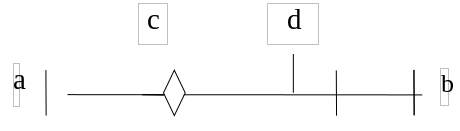
\includegraphics[width=50mm]{./imgs/fig6.jpg}
%\caption{I}
\end{figure}

Ou seja, o momento, entre dois instantes, em que o mundo se torna
visível, o ponto de encontro entre ``isto e aquilo'' (veja"-se o poema
``Nãoagora''). É assim que o poeta se explica em seu diário
(\textsc{kharms}, p. 95):

\begin{quote}
Se a verdade inteira se expande ao longo da linha \emph{ab}, então o
indivíduo só pode ver uma parte, a que não vai além de \emph{c}, o
limite do possível. (\ldots{}) {[}Valendo"-se da alteração do estado
normal de consciência{]}, certas pessoas podem estender sua percepção a
diferentes partes da verdade universal, por exemplo, até \emph{d}, mas
dificilmente elas terão uma compreensão real do que tiverem ``visto'',
pois terão conhecido apenas duas partes do mundo desconectadas uma da
outra: \emph{ac} e \emph{d.} A verdadeira compreensão lhes adviria do
conhecimento da verdade de \emph{a} até \emph{b}. (\ldots{}) Creio que
existam possibilidades, embora ocultas, de captar a verdade, não
escavando suas partes separadas, mas movendo"-se suavemente além dos
limites do possível \emph{c}, compreendendo a distância em sua
inteireza.

\begin{flushright}
(novembro de 1926)
\end{flushright}
\end{quote}

Embora tenha sido Drúskin, em 1933, a encontrar a expressão ``certo
equilíbrio com uma pequena falha'' (\emph{parvum peccatum}) --- que no
gráfico seria representado pelo obstáculo \emph{c} --- à qual ---
justamente --- atribuiu um matiz religioso (o protótipo da pequena falha,
no caso, seria Cristo feito homem, Deus tornado real, a imperfeição
somente através da qual é possível compreender a perfeição), o conceito
é arquetípico. (Veja"-se de \textsc{calvino}: 1997, \emph{Um assunto
encerrado}, em que o autor interpreta o fato de os indígenas sempre
deixarem um fio solto em seus tecidos).

Kharms retoma essa problemática em várias de suas miniaturas. Veja"-se
particularmente o episódio"-obstáculo da fada em ``Sobre o equilíbrio'',
de 1934. Por sinal, Jaccard (\textsc{jaccard}: 1995, p. 162) explica por
essa estruturação de ``certo equilíbrio'' o princípio característico da
assimetria que rege a poética de Kharms. Muitas, com efeito, são as
características de sua poética, que, em muitos aspectos fundamentais, é
decorrência de suas meditações filosóficas. Reduzir o objeto à soma de
partículas para poder integrá"-las ao todo, graças à ordem que a Arte
imprime, faz com que sua poética implique a ruptura, como fase
preliminar.

Quando algumas de suas convicções coincidiam com as de personalidades
que ele estimava, Kharms rejubilava"-se. ``Em tudo o que eu faço, eu sou
o criador de uma forma minha no mundo'' --- diz ele, ecoando Bakhtin.
Deslocamento, fluidez, deformação estão entre os fenômenos mais
conspícuos de sua poesia, coincidindo com a visão de Iúri Tyniánov, o
crítico formalista que ele mais apreciava. O intuitivo e o
\emph{transracional} que ele praticava são alguns dos pontos"-chaves de
Khlébnikov, o mestre do futurismo russo por quem tinha especial
predileção. Retirar a palavra do âmbito de sua distribuição normativa e
introduzi"-la num contexto não convencional (a não coincidência de
palavra com coisa), de modo que a palavra se torne livre, assumindo
significados diferentes, tem ligação com a importância que Malévitch
dava à ``situação'' do objeto, mais que à sua essência. O objeto deixa
de ter contornos definidos --- dizia o pintor --- ``e se espalha no
macrocosmo, tal como a palavra que, livre da causa"-efeito
lógico"-gramatical se ergue acima de constrangimentos''.

Como foi dito, Kharms, desde a época do Instituto Eletrotécnico,
desenvolveu estudos de numerologia, que, por ocasião de seu desterro em
Kursk, o levaram a profundas reflexões filosóficas. ``O infinito é a
resposta para todas as questões'' --- diz ele. ``A única pergunta que
merece ser colocada é: o que é o infinito?'' E o zero, que, não tendo
começo, não pode ter fim, permite"-lhe uma série de equiparações
inclusive com Deus: Religião = Harmonia + Deus = zero; Arte = Harmonia =
Ritmo e Beleza = zero; o que lembra o Deus"-zero suprematista de
Malévitch. No grau zero da criação, as palavras, como os sons, voam e
ressoam.

À divindade Kharms sempre apelara nos momentos difíceis à espera de
algum milagre, que não viria. Muitas passagens de seus diários, como foi
visto, se encerram com uma espécie de invocação salvadora --- uma espécie
de fórmula ---, que se transformará em constatação no fim de sua
atormentada existência: Deus deu"-lhe os melhores dotes e a vida
obrigou"-o a rastejar nas piores baixezas.

Os escritos de que consta este livro, de uma comicidade grotesca e
alógica que desconstrói um mundo tão parecido com o nosso mas que não
pode deixar de nos surpreender, custaram a internação, a prisão e a
morte a um jovem autor, hoje considerado um dos máximos representantes
da literatura do absurdo, entre os mais lidos e os mais publicados no
Ocidente.

Bibliografia

\versal{CALVINO}, Italo. \emph{Assunto encerrado -- discursos sobre literatura
e sociedade}. Tradução Roberta Barni. São Paulo: Companhia das Letras,
2009.

\versal{CHARMS}, Daniil. \emph{Casi}. Organização, tradução e posfácio
Rosanna Giaquinta. Milão: Adelphi, 1990. (\textsc{giaquinta}: 1990)

\versal{CHARMS}, Daniil (org. trad. e posfácio Paolo Nori). \emph{Disastri.}
Turim: Einaudi, 2003. (\textsc{nori}: 2003)

\versal{JACCARD}, Jean"-Philippe. \emph{Daniil Harms et la fin de
l'avant-garde russe}. Berna: Peter Lang, 1991.

\_\_\_\_\_\_\_\_\_\_ \emph{Daniil Kharms i koniéts rússkogo
avangarda}. São Petersburgo: \emph{Akademítcheskii proekt}, 1995.

\versal{KHARMS}, Daniil. \emph{I am a Phenomenon out of the Ordinary −
The Notebooks, Diaries and Letters of Daniil Kharms}. Organização,
tradução e introdução: Anthony Anemone e Peter Scotto. Boston: Academic
Studies Press, 2013. (\textsc{kharms}: 2013)

\_\_\_\_\_\_\_\_\_\_ \emph{Sobránie Sotchiniénii v dvukh
tomakh}. Moscou: Zebra E, 2010.

\versal{OSTASHEVSKI}, Eugene (org.). \emph{\versal{OBERIU} -- An Anthology of
Russian Absurdism}. Illinois: Northwestern University Press, 2006.

\versal{ROBERTS}, Graham. \emph{The Last Soviet Avant-garde}. Nova York:
Cambridge University Press, 1997.

\versal{YANKELEVICH}, Matvei (org.). \emph{Today I Wrote Nothing.} Nova York:
Overlook Duckworth, 2007.

\part{contemporâneos}

\chapter{Vladímir Nabókov: arte duradoura e talento individual}

Não por nada a primeira lição de literatura russa de Vladímir Nabókov
(1899--1977) reunida, com nove outras, no livro \emph{Lições de
literatura russa} (Três Estrelas, 2014), tem como fecho o poema
``À maneira de Pindemonte'', de Aleksandr Púchkin (de quem Nabókov
também verteu primorosamente para o inglês o famoso romance em versos
\emph{Evguêni Onéguin}, transformado em ópera com música de
Tchaikóvski); em poucas linhas, o poema sintetiza o credo de Nabókov ---
seu individualismo sem concessões e a relação conflituosa que se trava
entre o autor e o mundo:

\begin{verse}
Não responder a ninguém, ser seu próprio \\
vassalo e senhor, só agradar a si mesmo. \\
Não curvando a espinha, nem sua vontade \qb{}íntima, \\
nem a consciência (\ldots{}) e sentindo a alma \\
derreter no calor dos desígnios inspirados \qb{}do homem\ldots{}
\end{verse}

Dito isto, que se manifesta em suas opiniões quanto ao regime, aos
censores e aos escritores russos, resta deleitar"-se com suas análises
extraordinárias das obras dos autores russos do século \versal{XIX}, seus
favoritos, não apenas porque representam o pináculo da literatura russa,
mas também, --- conforme repara o prefaciador Fredson Bowers --- porque
lhe permitem se contrapor ao utilitarismo dos críticos sociais do século
anterior e dos escritores soviéticos que lhes sucederam.

Em particular, neste livro, ele trata de Gógol (\emph{Almas mortas} e
\emph{O capote}), Tolstói (\emph{Anna Kariênina} e \emph{A morte de Ivan
Ilitch}), Tchekhov (\emph{A dama do cachorrinho}, \emph{No fundo do
barranco} e \emph{A gaivota}) --- autores que admira; de Turguêniev
(\emph{Pais e filhos}) --- que aceita com reservas, justamente pelo apelo
ao elemento social, (ao qual Tchekhov, dono de ``toques leves e de
pequenos e inesperados meandros'', sempre resistiu), por suas pausas
tradicionais para o esboço biográfico das personagens e por saciar por
completo a curiosidade do leitor com seus epílogos; de Dostoiévski
(\emph{Crime e castigo}, \emph{Memórias do subsolo}, \emph{O idiota},
\emph{Os demônios} e \emph{Os irmãos Karamázov}) --- que critica: ``Minha
posição em relação a Dostoiévski é curiosa e difícil. Em todos os meus
cursos abordo a literatura a partir do único ponto de vista que me
interessa --- a saber, o da arte duradoura e do talento individual. Dessa
perspectiva Dostoiévski não é um grande escritor, ao contrário, é
bastante medíocre --- com lampejos de excelente humor mas, infelizmente,
separados por oceanos de platitudes literárias''.

Por outras perspectivas que o leitor terá o prazer de percorrer, porém,
reconhece"-lhe méritos, entre os quais o de saber admiravelmente reunir
farsa e tragédia, e de ser um dramaturgo \emph{manqué}. Finalmente
Gorki, que é assim desancado: ``sentindo que precisava encontrar alguma
compensação pela pobreza de sua arte e pelo caos de suas ideias, ele
sempre buscou os assuntos chocantes, o contraste, o conflito, a
violência, a crueldade''.

Quanto a Tolstói, tal como Nabókov pertencente à antiga nobreza
(conhecera"-o com o pai, quando criança), o considera o maior escritor
russo. Para ele, é o exemplo da perfeita estrutura temporal da obra, que
flui como real, juntamente com o tempo do leitor; do domínio som/sentido
(comum também a Gógol, o máximo representante da imaginação literária
eficaz e que não por nada chamou ``poema'' a seu \emph{Almas mortas}),
e da refinada arte dos detalhes que confluem para um mesmo fim (não se
esqueça que Tolstói é um autor que gosta de defender alguma tese em suas
obras), no caso de \emph{Anna Kariênina}, para os males do adultério.

Nas aulas sobre escritores ocidentais que ele ministrou, igualmente, em
várias universidades norte"-americanas, Nabókov ia direto para o estudo das
obras de seus favoritos, explicando"-as com diagramas e com citações
nevrálgicas (era formado em literatura francesa, além de conhecer
perfeitamente o alemão, e, com \emph{Lolita}, foi considerado um dos
mestres de língua inglesa). Entretanto, quando tratava de escritores
russos, dirigindo"-se a um público que desconhecia sua obra e sua
cultura, apresentava um resumo biográfico e uma visão geral do ambiente
e das obras do escritor, antes de passar à análise mais aprofundada das
obras escolhidas, que é o que mais o interessava.

Conforme é sabido, além de escritor e entomologista (tinha por
\emph{hobby}, desde a infância, colecionar borboletas, e em museus
norte"-americanos há espécies por ele descobertas), Nabókov era um inveterado
jogador, estudioso e preparador de problemas de xadrez. ``Em xadrez,
(\ldots{}) há os recursos como o avanço, o recuo, o bloqueio, o desbloqueio e
assim por diante, mas só quando são combinados de uma certa maneira é
que o problema se torna satisfatório'' --- diz Nabókov em sua
autobiografia (\emph{A pessoa em questão}, Companhia das Letras, 1994,
também traduzida como \emph{Fala, memória}, Alfaguara, 2014). Pois bem,
para ele, esses ``recursos'' são, em literatura, o uso e a combinação
dos detalhes: o domínio dos detalhes, ao mesmo tempo científico e
artístico, era a chave com que o leitor inteligente desvendava o segredo
do funcionamento das obras"-primas. ``Nos meus tempos de professor,
esforcei"-me para oferecer aos alunos de literatura a informação exata
sobre os detalhes, sobre as combinações de detalhes que produzem a
centelha sensual sem a qual o livro é algo morto'' (cf. \emph{Introdução}
de Fredson Bowers às \emph{Lições de literatura russa}).

Vejamos, para terminar, alguns exemplos de como os detalhes em
\emph{Anna Kariênina} de Tolstói funcionam como chave para a
interpretação da obra. No trem de volta a São Petersburgo, depois do
encontro fatal com Vrónski, Anna está lendo um livro, e a criada, que a
acompanha, tem ``as mãos largas enfiadas em luvas de lã, uma das quais
rasgadas na ponta de um dos dedos'' (``Reparem'' --- diz o
professor, entre parênteses, --- ``o pequeno defeito
correspondendo ao transtorno no estado de espírito de Anna'').
Sempre no vagão do trem: ``Notem que o quente e o frio estão se
alternando também no vagão"-dormitório'' e assim, num crescendo, até
analisar o sonho duplo (de Anna e de Vrónski) em que aparece o mesmo
anão maltrapilho, que Tolstói, antifreudianamente, analisa como sendo o
símbolo do pecado de ambos. ``de seu pecado imundo e deformador da alma
---, as duas imagens se mesclando num clarão funesto''.

\chapter{Viktor Chklóvski: \emph{Viagem sentimental}}

As peregrinações de Viktor Chklóvski (1893--1984) --- escritor e teórico
literário que há alguns anos vem sendo reavaliado (enaltecido) pela
crítica --- por Petersburgo, Galícia, Pérsia, Sarátov, Kiev,
Petersburgo, Dnieper, Petersburgo, Berlim, entre 1917 e 1922 (o roteiro
é dado por ele mesmo), realizam"-se ao longo de dois eixos --- o das
lembranças e o da atualidade (um esboço de diário) --- que, por vezes,
se interceptam, fazendo com que a ação seja submetida a curiosas
digressões instantâneas. Tanto o título \emph{Viagem sentimental}, como
o método (retardamento, \emph{flash back}, digressões, associações
irônicas) aludem à obra do escritor e clérigo anglicano irlandês
Laurence Sterne, principalmente a \emph{A vida e opiniões de Tristram
Shandy} (1759), que tanto inspirou também nosso Machado de Assis. É para
esses deslocamentos temporais e factuais e para a perspectiva cambiante
que eles provocam que o leitor deve estar preparado, para apreciar
devidamente esta \emph{Viagem}, onde os fatos imperam, narrados num
estilo conciso, quase telegráfico, e que --- apesar de descreverem
episódios terríveis dos anos da \versal{I} Guerra, da Revolução Russa, da Guerra
Civil e, finalmente, do Exército Vermelho --- não deixam de ter seu
lirismo e sua graça, mesmo que macabra: ``Um soldado que me contava um
linchamento exprimiu"-se assim: ` Então o morto falou'\ldots{} `O morto falou,
como assim?' `Sim, aquele que iam matar de qualquer jeito, falou'\ldots{}''

Historicamente, são três os livros que se sobrepõem nessa \emph{Viagem}.
O primeiro \emph{Revolução e front}, é redigido em 1919 e cobre o ano de
1917, quando Viktor servia como instrutor e reparador de carros
blindados e participava, como comissário de guerra, do Governo
Provisório, que tinha Kérenski como ministro da Guerra. Nesses últimos
meses da participação da Rússia na \versal{I} Guerra Mundial, Viktor viajou para
a Ucrânia e para a Pérsia (Irã, a partir de 1934), argutamente
descritas, com seus habitantes, nas páginas da \emph{Viagem}. É na
Pérsia que ele conhece Lazar Zervantov, comandante de bateria nascido na
Assíria (região do alto rio Tigre, no norte da Mesopotâmia --- atual
norte do Iraque) que se
torna uma personagem heroica no final da \emph{Viagem} e com quem Viktor
assina o \emph{Epílogo}: final do livro \emph{Revolução e front}. E é na
Pérsia que Viktor fica sabendo da Revolução de Outubro que, num de seus
primeiros atos, encerra a participação russa na \versal{I} Guerra e desocupa
militarmente a Pérsia. (Os velhos rancores entre turcos, assírios,
curdos e persas renascem, com isso, e todos combatem contra todos, até
que os assírios fogem, rumo a Bagdá, abandonando mulheres e crianças,
contará Lazar, no fim da \emph{Viagem}).

Após a dissolução da Assembleia Constituinte, em janeiro de 1918,
Chklóvski apoia o partido Socialista Revolucionário (\versal{S. R.}), mantendo"-se
fiel a Kérenski --- que descreve cruamente, juntamente com tantas outras
figuras --- e se envolve na frustrada revolução antibolchevique do verão
de 1919. Com a descoberta do plano, muda"-se para Saratov onde escreve
ensaios literários que irão compor seu livro já clássico, \emph{Sobre a
teoria da prosa} (publicado em 1925). De volta a Petersburgo (na época, Petrogrado), casa"-se com Liússia, a quem dedica a \emph{Viagem}, e passa a lecionar no Instituto da História da Arte. De
1920 a 1922 participa do \versal{OPOIAZ}, círculo dos formalistas e futuristas
petersburguêses, faz parte da redação do periódico \emph{Lef}
(\emph{Front de Esquerda da Arte}) e discute sobre a Escola Formalista
que, perseguida pelo ``Realismo Socialista'', ele haveria de renegar,
em 1930.

Em fevereiro de 1922 sai, em Berlim, um panfleto de um antigo
participante do \versal{S. R.} citando seu nome. Em março Viktor é procurado e
foge rocambolescamente para a Finlândia.

Dois meses depois, começa a escrever \emph{Escrivaninha} que, juntamente
com trechos do \emph{Epílogo}, forma a \versal{II} parte da \emph{Viagem
sentimental}, terminada em Berlim no começo de 1923.

O aporte de Chklóvski, em termos de literatura, é bastante curioso.
Deve"-se saber (conforme explica no posfácio Galin Tihanov), que --- em
1919 --- ele participou de um projeto de Maksim Gorki, em Petrogrado,
chamado ``Literatura Universal'' que, além dos clássicos ocidentais,
propunha"-se a traduzir para o russo obras da literatura asiática, do
Oriente"-médio e da América latina (do projeto participavam grandes
nomes, como I. Zamiátin, N. Gumilióv, K. Tchukóvski, etc.). Só que
Chkóvski, por ser monolíngue, nada traduziu, mas foi incumbido por Gorki
de dar palestras sobre teoria literária a um público jovem, com quem
analisou o fenômeno do ``estranhamento'' (ou desfamiliarização) nas
obras de Cervantes e de Laurence Sterne, no nível da composição (e não
da linguagem, pois trabalhava com obras traduzidas, e isso o contrapôs a
Roman Jákobson que trabalhava principalmente no nível da linguagem
original). Nessas obras e nas de Tolstói levantou dezenas de
procedimentos que descreveu, depois, em seu livro \emph{Sobre a teoria
da prosa}, onde há uma série de outros ensaios sobre construção
literária. São esses procedimentos que ele utiliza em \emph{Viagem
sentimental}, como dissemos, de seu próprio jeito, muitas vezes irônico
ou paradoxal.

Nos paralelismos, veja"-se o tipo de comparação à qual ele recorre:
``Percorri toda a estrada de Uchnué a Petersburgo junto com soldados
fugitivos, rato malhado''. Ou então: ``A massa agia como os arenques ou
as carpas na iminência de desovar\ldots{}''

Nas digressões, então, o estranhamento é maior ainda. Algo como o que os
russos jocosamente definem como ``\emph{Diádia v Kíeve, a na ogaródie
buziná}'' (O tio está em Kiév, mas a sorva está na horta): ``\ldots{} Se então
nos tivessem perguntado: `Com quem estão, afinal? Com Kornilov, com
Kaledin ou com os bolcheviques?' Task e eu teríamos escolhido os
bolcheviques. À pergunta: ` Preferes ser enforcado ou esquartejado?'
Arlequim responde: `Prefiro a sopa'.''

De volta à \versal{URSS}, dedica"-se a livros de memórias (\emph{Zoo, ou cartas
não sobre o amor}, 1923 --- sobre sua relação com Elsa Triolet, irmã de
Lila Brik, o amor de Maiakóvski e \emph{A terceira fábrica}, 1926) e
trabalha como editor de filmes e roteirista. ``Durante o período
stalinista tive muitos aborrecimentos, mas não fui nunca detido; creio
que é porque eu já havia escrito tudo sobre mim em \emph{Viagem
sentimental} --- ironiza ele --- e não havia mais nada que pudesse ser
descoberto a meu respeito''. Escreve copiosamente até o fim,
reavaliando seus escritos da juventude e destacando"-se no estudo sobre
Serguei Eisenstein. Em 1956 casa"-se novamente e, três décadas depois,
morre em Moscou, com 91 anos de idade.

\chapter*{Um escritor russo na América -- Dovlátov: \emph{Parque Cultural} e \emph{O ofício}}

\addcontentsline{toc}{chapter}{Um escritor russo na América -- Dovlátov}
\hedramarkboth{Um escritor russo na América -- Dovlátov}{}

Serguei Dovlátov (1941--1990) é um nome importante não apenas na
literatura russa de hoje, mas também na dos \versal{EUA}, para onde emigrou (1978) e se tornou famoso como fundador do jornal \emph{O novo
americano}, foi reconhecido pelas mais prestigiosas revistas (\emph{New
Yorker} e \emph{Partizan Review}), lançou 12 livros, e lhe foi dedicada
uma rua (\emph{Sergei Dovlatov way} --- no Queens).

Já o parque ``Serguei Dovlátov'' que lhe foi dedicado na Rússia de
hoje, quando se tornou um autor icônico, entre os mais queridos, tem a
ver com esta curiosa novela, uma das mais comicamente ferinas que se
possam ler na literatura russa atual. Acontece que na Rússia de Púchkin
(1799--1837) havia uma propriedade, na região de Mikháilovskoie (perto de
Pskov --- norte do país), onde o grande poeta costumava passar suas
férias (e exílio), que na época da \versal{URSS} foi transformada em
\emph{Parque Cultural} e monumento histórico. Um parque, onde foi
recriado o ambiente da época do poeta nacional, retocado (leia"-se
``fajutado''), aberto à visitação pública, e onde Dovlátov trabalhou
como guia turístico pouco antes de emigrar, parque esse que para Borís
Alikhánov (seu \emph{alter ego}, na novela) é uma alegoria da própria
vida na \versal{URSS}. Mas descrita com tanto humor (cáustico) pelo protagonista
e narrador Alikhánov, que se autoironiza (como o Humbert Humbert de
\emph{Lolita} ou o nosso Serafim Ponte Grande) dizendo, com a sua
inconveniência politicamente incorreta, disparates que muitos ``pensam,
mas não dizem'', entremeados por generalizações comuns ao mundo inteiro
(liberdade, amor, morte, impostura, vícios: em especial --- sexo e
bebida), expressas com uma hilariante ingenuidade \emph{non"-sense} que
conquista a simpatia do leitor a cada página.

Na verdade, como muitos artistas, o autor recria nas obras, publicadas
após sua emigração (todas, tirante alguns contos em \emph{samizdat} que
foram bem recebidos e que, apesar de desconstruírem o mito soviético,
nunca provocaram rejeição), fatos e figuras das etapas de sua vida
real. Seu malogro inicial na literatura oficial foi, inicialmente, ele
ter passado a constar, em 1968, de uma ``lista negra'' (dos
participantes do ``Sarau da juventude criativa de Leningrado'') --- coisa
que ele só descobriu mais tarde: ``Na União Soviética eu não era
dissidente. (A bebedeira não conta). Eu apenas escrevia contos alheios à
ideologia\ldots{} Publicam qualquer um, menos eu. As pessoas vendem a alma ao
diabo, eu a dei de graça\ldots{}''

Sua infância/juventude/maturidade aparecem nos contos de \emph{Os
nossos} (1977): a família, os amigos; \emph{A mala} (1986): o resumo
de toda sua vida na \versal{URSS}; \emph{O ofício} (1985): este, sobre sua
``carreira'' na \versal{URSS} e na América, já publicado em português; \emph{A troca} (1981): período
de 5 anos em que trabalhou em Tallin como jornalista, encerrado por
outro malogro completamente casual; \emph{A zona} (1982): seu serviço
militar como membro da ``tropa da prisão''; e nas novelas curtas
\emph{A estrangeira} (1986): sobre a emigrada Mússia Tataróvith; \emph{A filial} (1990), etc.

O eixo de \emph{Parque Cultural} (1983) é a separação da mulher do
narrador (Tânia, na novela) que emigra com a filha para os \versal{EUA} (o pai do
ex"-marido é judeu) bem no momento em que, apesar da bebedeira e de uma
série de quiproquós com figuras impagáveis (os turistas, que às vezes
desmaiavam de tensão, a metodologista, de corpo indistintamente feio, o
senhorio bêbado, o guia preguiçoso\ldots{}), Alikhánov achava ter conseguido
uma certa harmonia. ``Decidi ponderar tudo com calma. Tentar dissipar a
sensação de catástrofe, de beco sem saída. A vida se desenrolava como
imenso campo minado. E eu estava bem no meio dele. Era necessário
dividir este campo em setores e pôr mãos à obra\ldots{}''. Mas os fatos não o
permitem, ele cai em depressão, volta ao vício e vê"-se acossado pela
censura que sempre, nos momentos culminantes de sua tão desejada
carreira literária, reúne indícios para não publicá"-lo. Estamos na
véspera das Olimpíadas de 1980, época em que se procurava fazer com que
os ``indesejáveis'' saíssem do país e --- de fato ---, na vida real,
apesar de não querê"-lo (``é possível sobreviver e continuar escrevendo
longe de seu leitor e de sua língua?''), Dovlátov, com a mãe e a
cachorrinha de estimação, acaba deixando o país, rumo aos \versal{EUA}, onde, como
previra seu amigo Joseph Bródski que o admirava, terá sucesso de crítica
e de público.

Quando o escritor morreu, em 1990 (de uma parada cardíaca, consequência
da bebida que nunca abandonou), a Rússia lançou oficialmente sua
primeira coletânea de contos. O sucesso foi estrondoso. Sua obra
completa foi publicada em três volumes (1995), saíram pesquisas,
biografias, memórias, filmes, congressos, documentários sobre ele e sua
obra. A casa alugada pelo escritor perto do \emph{Parque Cultural}, que
se encontra na aldeia que no livro aparece com o nome de \emph{Sosnovo,}
tornou"-se sede de um museu no parque que hoje leva seu nome.

Quanto a \emph{O ofício} (Kalinka/Hedra, 2018), trata-se de um livro (publicado primeiramente em New York, em 1985), do escritor emigrado, já conhecido no Brasil pelo hilariante Parque Cultural(Kalinka, 2017).

``Ler Dovlátov é algo leve. Ele como que não reivindica atenção, não insiste em suas conclusões ou observações sobre a natureza humana, não as impõe ao leitor. Eu devoro seus livros em três ou quatro horas de leitura ininterrupta: justamente porque é difícil escapar de seu tom despojado. Ao ler seus contos e novelas, invariavelmente nos sentimos gratos pela ausência de pretensão, pelo olhar ponderado sobre as coisas\ldots{}''

Assim escrevia o poeta Joseph Bródski  ``Ao Seriôja Dovlátov'', dois anos após a morte repentina deste numa ambulância em 1990, num elogio ao amigo, também emigrado nos \versal{EUA}, onde Dovlátov, a partir de 1979, publicara nada menos que doze livros. E é isso é o que sentimos nós, leitores, ao lermos esse seu \emph{O ofício} que, na sua primeira parte, descreve ``alguns dias na vida do jovem Serguei Dovlátov''. Seu entourage, a boemia leningradense e suas vicissitudes, os cafés e as redações que não queriam saber de publicar seus escritos, seus galanteios, suas bebedeiras. 

Há caracterizações engraçadíssimas no ``livro invisível'' (é assim que ele chama a primeira parte), cujos comentários ele reserva para si próprio, nas considerações que ele denomina ``Solos na Underwood'': 

\begin{quote}
Pelo bulevar, ao longo de banquinhos amarelos, diante das lixeiras de gesso, caminha um homem de baixa estatura. Seu nome é Anatóli Náiman.
Suas pernas lestas são revestidas por jeans claros americanos. Em seus movimentos se nota a graça de um jovem príncipe. Náiman é um cowboy intelectual. Ele aperta o gatilho antes de qualquer oponente. Seus chistes afiados estão repletos de veneno. 

\begin{center}
\versal{SOLO NA UNDERWOOD}\\
\end{center}
Uma mulher no bonde diz a Náiman: \\
``Ah, não me toque!'' \\
``Não faz mal, depois vou lavar as mãos\ldots{}''
\end{quote}

Ou então, outro \versal{SOLO}:

\begin{quote}
``Tólia'', digo a Náiman, ``vamos visitar Liova Rýskin''. \\
``Não vou. Ele é um  tanto soviético''. \\
``Como soviético? Você está equivocado!'' \\
``Então é antissoviético. Qual a diferença?\ldots{}''
\end{quote}

Paradoxos dessa natureza tornam não menos divertida (e mesmo assim, percuciente) a descrição, na segunda parte do livro, de suas experiências na América, muito próximas da autobiografia. Querendo publicar um novo jornal russo (``O Espelho''), ele e um grupo de companheiros emigrados resolvem procurar um financiador.

``Na casa da tal Cíntia'' --- prosseguiu Móker --- ``volta e meia aparece um italiano. Eu topo toda hora com ele no elevador. Por sinal, ele só vai visitá-la de dia. Daí Cíntia imediatamente corre as cortinas. Que conclusão podemos tirar?''

(\ldots{})

--- ``Daí podemos concluir que Rizzo é dono de um estabelecimento noturno. Por isso faz amor apenas de dia. E todos os estabelecimento noturnos são controlados pela máfia''.

Os amigos marcam encontro com o ``mafioso'' na esquina da Dezessete com a Quinta Avenida e, depois de vários coquetéis expõem ao italiano seu projeto.

\begin{quote}
``Não tocaremos em seu programa ideológico'' --- diz"-lhe Móker. ``Nós apreciamos lutadores honestos, pouco importam suas convicções. Ouvi falar muito de sua organização. Pessoalmente, os objetivos e, especialmente os métodos dela não me são familiares. Mas estou habituado a honrar a firmeza e a valentia em qualquer forma de manifestação\ldots{} Estou ciente que as leis da organização são severas''.

Rizzo assentiu com a cabeça, orgulhoso: --- ``Sim, a organização liquida instantaneamente quem a trai. Não é de se invejar o destino de quem descumpre a palavra dada à organização\ldots{}''
\end{quote}

Qual não é o espanto da turma quando, ao falarem em dinheiro, assim responde Rizzo:

-- ``Claro, eu falarei com o Rafael. Ele administra o caixa do partido. Francamente, duvido que aceite. Rafael é um pouco conservador. Estou certo que ele é muito mais conservador do que seu ídolo, Trótski. Nossa facção de maoístas de esquerda se encontra bem distante do centro\ldots{}''

Sempre à procura do capital inicial para o jornal, Lémkus, outro companheiro que também escrevia para o velho (e único) jornal russo local \emph{Palavra e ação} artigos como ``Como encontrar Deus'', explica:

\begin{quote}
--- ``Vocês simplesmente não conhecem a vida na América. Aqui existem métodos de enriquecimento comprovados e dentro da lei. O que poderia ser mais simples? Você anda pela luxuosa avenida Madison. Em sua direção vem um cachorro, um puro dobermann. Você diz: `Ah, que cachorro bonitinho!'. E, com um movimento rápido, dá-lhe um piparote no nariz. O dobermann engancha sua perna. Você desmaia. Constatam um choque nervoso. Você telefona para um bom advogado. Processa o dono do dobermann. Pede uma indenização por danos físicos e morais. O dono-milionário assina um cheque de pelo menos vinte mil\ldots{}''

--- ``E se for verificado que o cachorro pertence a um mendigo? Será que na Broadway há poucos aleijados negros com dobermanns?''

--- ``Não estou falando da Broadway. Estou falando da Madison. Lá só dá milionário\ldots{}''
\end{quote}

Apesar do sucesso de público e de crítica do novo periódico, finalmente financiado por Larry (``O objetivo da gazeta será aproximar os leitores do Deus judeu e da tradição sionista'') e de seu fracasso financeiro (a redação acaba incendiada), o narrador em primeira pessoa consegue, graças à ajuda da atraente tradutora, Lynn Farber, ter contos seus  publicados pela \emph{New Yorker}. E mais, há um agente literário, Charlie, que lhe encomenda vários romances.

\begin{quote}
Eu só pensava: acontece cada coisa! Um americano, falante de outra língua, ainda por cima ``meio vermelho'', de esquerda, tornou"-se mais próximo e mais compreensível do que meus velhos amigos. As relações humanas possuem um quê de mistério\ldots{}
\end{quote}

\chapter*{Friedrich Gorenstein: \emph{Salmo}, um romance"-meditação sobre os quatros flagelos do Senhor}

\addcontentsline{toc}{chapter}{Friedrich Gorenstein: \emph{Salmo}}
\hedramarkboth{Friedrich Gorenstein: \emph{Salmo}}{}

Intrigante e apaixonante é \emph{Salmo} (1975) de Friedrich Gorenstein (1932--2002), autor judeu russo praticamente desconhecido no
Brasil (apesar de ter sido roteirista, entre outros, de \emph{Soláris}
e \emph{Andrei Rubliov} de Tarkóvski). O livro é, como quer o autor,
``\emph{um romance"-meditação sobre os quatro flagelos do Senhor''} e,
por sua temática, construção e estilo é, entre suas obras"-primas
(\emph{Tchok"-tchok -- romance erótico"-filosófico, Expiação, A casa com a
torre, O lugar)}, a que pode ser considerada a mais importante.

O romance narra nada menos que a vinda do Anticristo em 1933, numa
pequena aldeia da Ucrânia e suas peripécias pela Rússia stalinista até
1973, ano em que desparece. As etapas de suas andanças são pontuadas por
projeções entre profecias da Bíblia e acontecimentos realistas da Rússia
do século \versal{XX} (deskulakização, grande fome na Ucrânia, invasão alemã,
repressões stalinistas, o \emph{homo sovieticus}, o lugar do judeu na
sociedade soviética), época e lugar em que se desencadeiam os flagelos
impostos por Deus aos homens, como punição por seus terríveis desmandos.

Cada um dos capítulos descreve um flagelo (a espada, a fome, a doença e,
particularmente, a luxúria --- ``o animal selvagem que ao dilacerar,
frutifica'') e seus envolvidos que o Anticristo não perde de vista. A
estrutura de cada capítulo é curiosa: um preâmbulo teológico"-filosófico
em que ora se defrontam o Antigo e o Novo Testamento, ora Moisés, que
veio para amaldiçoar os pecadores e defender as vítimas, e Cristo (o
irmão do Anticristo), que veio para perdoar aos pecadores e acenar a
eles e às vítimas com a vida eterna, traído não apenas por Judas mas
pelos apóstolos que não o compreenderam e conspiraram contra ele, e pelo
``pântano cristão de questões metafísicas alheias ao Cristo''. Ora se
defrontam a concepção de mundo de Dostoiévski e a de Púchkin; ora o ateísmo e a fé,
ora a cultura ocidental e as verdades bíblicas, ora a poesia e a
história etc. Depois do preâmbulo há sempre uma parábola que descreve
numa linguagem muito viva as paixões e os instintos dos homens e das
mulheres (principalmente russos e judeus) que se entrelaçam e redundam
em fatos expostos com perspicácia e crueza total e implicam as
diferentes punições, acompanhados por digressões e interpretações do
autor e --- finalmente --- os vaticínios de um magistral deus"-ex"-machina:
o \emph{homúnculo} que Andrei (um dos filhos da luxúria do Anticristo)
consegue criar em seu laboratório graças a seus conhecimentos alquímicos
e à ajuda da profetisa Pelágia, filha adotiva e última amante do
Anticristo.

Ao homúnculo Andrei submete algumas questões que considera cruciais: Quais são
as maiores ideias do mundo? O que é mundo religioso e mundo filosófico?
Quais são os caminhos para se chegar a Deus? Como saber se uma ação é
boa ou má? O que é verdade? Qual a diferença entre o bem e a bondade?

Se as respostas do homúnculo são teoricamente incontestáveis, as
``mensagens'' do narrador que se entreveem atrás delas convidam à
discussão.

Uma das mais curiosas diz respeito ao ``caráter popular russo'', que
teria sido secado, esgotado pela consciência popular, ``através da qual
o povo começou a assumir a direção da história'': ``Quando o povo quer,
com sua consciência humilde, compreender seus instintos profundos,
forma"-se aquela filosofia de \emph{lubok}, de \emph{tchastuchka}, à qual
se curvam os eslavófilos da Rússia. Um criminoso desastrado ---
oposicionista ou governante --- eis o produto final da consciência
popular\ldots{} E --- continua Gorenstein ---

\begin{quote}
Se, no século \versal{XIX}, a Rússia conseguiu criar uma grande
cultura, foi porque as reformas de Pedro, o Grande, arrancaram os
intelectuais do povo, porque, explorando o frutífero oceano do instinto
popular, a cultura não foi escravizada pela consciência popular. Somente
mais tarde, mais perto do fim do século, graças aos esforços dos
intelectuais"-acusadores, a consciência popular começou a escravizar a
cultura, e os seguidores dos acusadores levaram esse processo até seu
limite.
\end{quote}

No que se refere à religião, um dos pontos de que o narrador parte é que
o homem é ``tolo, mau e miserável'' desde o momento em que, assumindo a
consciência, é expulso do paraíso. No entanto ele nasceu com o ``
instinto'' de Deus, que não é explicável nem pela razão, nem pela
inteligência: ouvir Deus falando a um arbusto só é possível ao artista.
A necessidade de Deus é a primeira prova da existência de Deus. Entre os
que foram salvos do dilúvio enviado por Deus (cuja obra ele mesmo
reconheceu ser imperfeita), os ímpios serão por Ele abandonados ---
``Nem todos os estilhaços da taça podem ser colados''---, mas Cristo
foi enviado para não abandonar os que Deus abandonou.

No que se refere particularmente aos judeus, este diálogo entre Pelágia
e o Anticristo é revelador:

\begin{quote}
--- Pai, mas como podem se salvar os perseguidos, como podem se salvar
aqueles que são odiados?

\noindent{}--- Para os perseguidores, Cristo é o Salvador, para os perseguidos, o
Anticristo é o Salvador. Para isso é que fui enviado pelo Senhor. Vocês
ouviram o que foi dito: amem os seus inimigos, abençoem quem os
amaldiçoa, façam o bem a quem os odeia e orem pelo bem dos que os magoam
e os perseguem. Mas eu lhes digo, amem não seus inimigos, mas o ódio dos
seus inimigos (\ldots{}) Pois o ódio de seus inimigos é a Marca Divina que os
abençoa (\ldots{}). Esse povo não se destaca em nada dos outros, e em nada é
melhor, mas com esse ódio invariável ele se destaca, e por causa desse
ódio ele é melhor.
\end{quote}

Religião à parte, mas focalizando aqui a relação judeu/russo numa das
parábolas do livro, o caso do crítico de arte Aleksei Iossífovitch
Ivólguin é emblemático. O avô dele conseguira trocar o sobrenome Katz por
Ivólguin, comprando"-o de um militar e Aleksei não só se sente agora
russo (``de passaporte''), mas --- num ímpeto do patriotismo que ele
teria, se fosse verdadeiramente russo --- chega a desprezar os judeus
``que não apreciam o pão russo, a hospitalidade russa\ldots{} Os ingratos\ldots{}
Ah, como ele os detesta!\ldots{}''

Pois bem, em 1952, ano do recrudescimento do terror stalinista em geral
e dos ataques antissemitas em particular, sua vida feliz termina e,
depois de vicissitudes cada vez mais acabrunhantes, em 1953 ele acaba
preso e morto justamente pela origem judia que ele havia tentado
repudiar.

A hostilidade dos outros lhe havia feito perder a consciência de seu
caráter judeu, mas ele o carrega como um fardo a ser rejeitado,
inclusive por não ter, em 1953, uma terra própria à qual se ligar, nota
a estudiosa Korine Amacher, em seu ensaio sobre Gorestein ``\emph{L'oeuvre de
Friedrich Gorenstein -- refus de soi, refus de l'autre dans la societé
soviétique}''. É essa rejeição que Gorenstein castiga, no romance que, no entanto, como a maioria dos escritos do autor, encerra,
no fim, uma nota positiva: 

\begin{quote}
Qualquer vida e qualquer destino, mesmo uma
vida amarga e um destino cruel, quando passa, deve se constituir num
Salmo. Louvar ao Senhor por ela ter acontecido, diferentemente das vidas
que não nasceram e dos destinos que não aconteceram. Qualquer vida,
mesmo amarga, é uma sorte e um privilégio\ldots{}
\end{quote}

\part{Estudos Teóricos}

\chapter{Dos diários de Serguei Eisenstein e outros ensaios}

Viatchesláv Vsiévolodovitch Ivanov, eminente professor universitário da
\versal{MGU} (Moscou) e da \versal{UCLA} (Los Angeles), crítico, semioticista,
antropólogo cultural e linguista de fama mundial, esteve em S. Paulo em
1990 (a convite do \versal{DLO/IEA} e com patrocínio da \versal{FAPESP}), ocasião em que
ministrou uma série de conferências e deslumbrou os ouvintes com sua
excepcional cultura. Falou sobre alguns de seus trabalhos como \emph{A
história da cultura mundial, o indo"-europeu e os indo"-europeus} (
obra em dois volumes pela qual, em parceria com um colega, obteve o
prêmio Lênin em 1988), \emph{A semiótica na Rússia e no Ocidente; Par e
ímpar: o funcionamento dos hemisférios do cérebro}. Dois dos trabalhos
ilustrados pelas conferências foram traduzidos para o português, por
equipes das quais participaram professores do Curso de Russo da \versal{USP} e, recentemente, reunindo estudos de
História da Cultura Mundial, de Mito e Linguagem, remontando dos
primórdios da civilização até os nossos dias e, principalmente,
analisando os arquivos inéditos do famoso cineasta Serguei Eisenstein e
encontrando ali elementos extremamente originais que ligam o cinema aos
outros sistemas de signos foi publicado o livro \emph{Dos arquivos de
Serguei Eisenstein e outros ensaios,} que analisaremos nesta resenha.

O livro, primeiramente publicado em 1976, em Moscou, é constituído por
cinco capítulos que podem ser lidos como estudos independentes mas que,
naturalmente, têm sua sequencia lógica e a suas ligações: a mais
conspícua delas sendo a presença constante do pensamento de Serguei
Eisenstein.

No primeiro, o estudo de ``As etapas primevas do desenvolvimento
dos sistemas de signos'', ou seja, a pré"-história da Semiótica, está
ligado a uma das grandes hipóteses da Antropologia Cultural, entendida
aqui como ``a ciência que estuda comparativamente diversos tipos de
cultura e as vias pelas quais esses tipos de cultura sofrem
transformações no processo de transmissão social da informação, de uma
geração a outra''. A hipótese seria a seguinte: dentro
das diferentes maneiras de se entenderem semelhanças pode"-se admitir que
muitas delas não se expliquem pelo modelo da continuidade histórica (o
\emph{continuum} da história), mas pela convergência de processos
históricos tipológicos, um de cujos modelos pode ser considerado o dos
ciclos de desenvolvimento. Ou, em outros termos: os resultados
históricos de certa continuidade, cuja ocorrência nos é visível, só são
avaliados com base em outra continuidade análoga no passado, com a qual
aqueles se identificam ou se correlacionam, em certo sentido.

A escola da Antropologia Cultural Russa conta com fundadores ilustres:
M. Bakhtin, V. Propp, F. Kameniétski, O. Freidenberg, L. Vigótski e
S. Eisenstein. Para eles era fundamental o \emph{princípio dinâmico,}
segundo o qual o pesquisador, começando por separar os segmentos mais
arcaicos na descrição sincrônica dos elementos ``não oficiais'' de
determinada tradição cultural, remonta gradualmente às fontes desta e
examina as vias de sua posterior transformação. Assim, elementos
(textos) orais, gestuais, ritualísticos e mitológicos comparados
permitem reconstituir a situação que precedeu os mais antigos textos
escritos da humanidade.

Um dos assuntos tocados neste primeiro capítulo serve de exemplo: a
situação folclórica original da ``proposta (enigmação) e
decifração"-do"-enigma''. Vladimir Propp e Olga Freidenberg caracterizaram
esta situação na versão trágica do mito de Édipo, em Sófocles. Avançando
pelo mesmo caminho, V. V. Ivanov propõe remontar às raízes linguísticas (
proto"-indoeuropeias) e mitológicas desse mesmo motivo e ir mais além:
perscrutar as raízes humanas universais dos enigmas relacionados com o
incesto que unem as tradições do Velho e do Novo Mundo. Assim, além das
fontes remotas, descobrem"-se também as causas mais tardias da
transformação da antiga estrutura.

Dada uma ideia geral, embrenhar"-se por essas trilhas heurísticas, apesar
\emph{et pour cause} da linguagem e das referências extremamente
rigorosas, é empresa altamente instigante. Pode"-se dizer que a cada
momento encontram"-se teses e comprovações surpreendentes. Sirva como
exemplo aqui uma tese de Bogatyriov: ``atos mágicos e fórmulas verbais
podem ter surgido ao mesmo tempo''. Estudando o papel fundamental das
palavras nas representações religiosas arcaicas, através da linguística
e da etnologia chegou a comprová"-lo na civilização dos Hititas. O
próximo passo foi verificar como o texto verbal antigo é inseparável do
ato ritual, num número significativamente grande de casos, instituindo o
assim chamado ``sincretismo primitivo''.

Além dele, Vesselóvski e Vygótski, levaram adiante esses estudos: se o
primeiro postulou que o mais antigo rito sincrético correspondia à
necessidade de uma catarse psico"-física o segundo, baseado no conhecido
princípio fisiológico do ``funil'' de Sherrington e nas suas próprias
investigações psico"-fisiológicas, estudou a união dessas formas
sincréticas catárticas primitivas com a arte posterior.

No estudo dos diferentes sistemas de signos (línguas, mitos, rituais,
etc.), a aproximação tipológica de um deles, tido como o mais arcaico,
a quaisquer fenômenos no interior de outro sistema semelhante é
justificada no caso desses fenômenos terem"-se sobressaído como
resquícios. Este é um dos princípios formulados por Vesselóvski quanto à
``racionalidade das contraposições tipológicas''. Entre suas
comprovações está todo o estudo dos rituais siberianos da ``caça ao urso'' onde, residualmente, está refletida a visão de mundo
dos povos da Idade da pedra.

Mas onde começa a entrar Eisenstein nisso tudo? Justamente no momento em
que Vesselóvski aprofunda a noção dos formalistas russos de que a
delimitação dos gêneros artísticos ``é sempre histórica, ou seja,
justificada somente para um determinado momento'', sendo --- os gêneros ---
resultado da evolução diacrônica do ato sincrético original, e
estabelecendo com isso um limite entre a poética contemporânea e a
poética ``sincrônica'' de Aristóteles.

Bakhtin e Eisenstein conseguiram desfazer a contradição entre poética
diacrônica e sincrônica, o primeiro baseando"-se na integração dos
``gêneros discursivos'' ligados a determinadas situações de comunicação,
o segundo introduzindo categorias aristotélicas no episódio da escadaria
de Odessa do \emph{Encouraçado Potiómkin}. Já está visível a atração
que Eisenstein sente não apenas pela totalidade em si, mas por uma
totalidade que represente a união dos contrários.

Outra hipótese cara a Eisenstein, a do caráter primeiro da técnica em
relação à arte (que nada tem a ver com o tecnicismo em si) e da
concepção técnica do estilo, não só não constitui de modo algum um
resultado dos últimos séculos, mas é verificada, segundo o relato de
V. V. Ivanov, em particularidades da terminologia indo"-europeia: ``a
criação de obras de arte vocabular [e de outras obras de arte, como é
de se esperar] era descrita mediante indicações técnicas que se referiam
inicialmente àqueles ofícios como a carpintaria, a tecelagem, a
urdidura''.

``Qual a base gestual que existe no fundo das significações das
palavras, dos desenhos, das representações pictóricas?'' Esta é mais uma
pergunta, respondida neste capítulo, que liga, por exemplo, os arquivos
de Eisenstein aos arquivos de Vygótski: ``Analisando os mais diversos
conceitos'' --- escreve V. V. Ivanov --- ``Eisenstein, que preencheu com
pesquisas etimológicas seus diários, procurava descobrir as ações
físicas (biológicas) nas quais aquelas representações se baseiam (\ldots{}).
Esta sua ênfase no gesto físico apresenta interesse à luz de novos
trabalhos sobre semântica, onde se supõe que a orientação física do
homem sirva de base para a descrição do seu mundo, que está fixada na
linguagem'' (cf. a ideia de Vygótski sobre a ``naive physic'').

Se o primeiro e o quarto capítulo do livro (que, partindo dos hinos
védicos em que está anagramado o nome impronunciável da divindade, passa
por Bach, o compositor favorito de Eisenstein, que anagramava seu nome
em suas composições e chega aos anagramas de Saussure) servem de
molduras refinadas para o pensamento de Eisenstein, o grande quadro se
encontra nos capítulos centrais. Neles V. V. Ivanos se baseou em duas
importantes obras do cineasta publicadas, até agora, apenas em
fragmentos, \emph{O método} (\emph{Methode}) e \emph{O problema básico} (emph{Grundproblem}) e das páginas, guardadas em arquivos não consultados
antes de Ivánov, de suas anotações e diários realizados durante as
filmagens de \emph{Que viva México}.

Acompanhando o fio alinhavado no começo de que o sincretismo
biológico"-social não aparece apenas nos sistemas primitivos, mas em
todos os sistemas de signos da arte, é em \emph{Grundproblem} e
\emph{Mehtode} que Eisenstein esboça sua teoria estética em uma
linguagem telegráfica (o que leva a crer que os livros e as anotações
fossem primeiramente um pro"-memória) onde os equacionamentos e as
alusões são organizados e comentados por V. V. Ivanov de maneira a tornar
a leitura sempre mais estimulante. Partindo do pressuposto de que a
juventude do cinema o liga às formas arcaicas da cultura, Eisenstein vai
ainda mais longe: para chegar ao movimento cinematográfico dedica"-se ao
estudo do tropismo das plantas, aos olhos dos insetos e dos répteis e à
imobilidade regressiva da máscara e, partindo dos níveis do movimento
fisiológico chega aos níveis da consciência. Ao longo de seu caminho
biológico"-dialético"-evolucional, próximo a um biologismo psicanalítico,
as descobertas são contínuas: todas elas encadeiam"-se para o que ele
caracterizou como sendo ``o problema fundamental'' da arte, ``a ascensão
aos mais altos níveis intelectuais e a descida, através da forma, nas
camadas do mais profundo pensamento sensorial''. Esse mergulho no
pensamento arcaico, pré"-lógico, representa a regressão, que deve ser
compensada pela progressão, para que se crie a obra de arte. Não há a
menor dúvida que a arte, para Eisenstein, está ligada ao diabólico, ao
arquetípico, ao mágico. De tanto meditar sobre seus limites, em seus
estudos sobre o êxtase, Eisenstein chegou a passar por uma verdadeira
crise. Acalmou"-o a ideia de que o artista mantém controle sobre esses
limites, enquanto que eles escapam ao doente. ``Os traços arcaicos
regressivos (especialmente os ligados ao sincretismo e à
indiferenciação iniciais) são patológicos, eles se prolongam nas etapas
seguintes, mas podem ser controlados pelo artista''.

A forma, então, age sensorialmente sobre o autor e o fruidor, porém
sobre o pano de fundo de uma grande unidade ou lei do comportamento
social, ou, melhor ainda, --- quando encontrada --- de uma lei cósmica ou
primordial. Quanto mais vasta essa lei, mais eficaz. As pesquisas do
cineasta nesse campo são as mais insólitas e as mais apaixonantes. Só
para enumerar algumas: o cinema de Walt Disney e a regressão ao mundo
animal; a passagem do mundo vegetal para o mineral e a forma
cristalográfica do ornamento; a auto"-punição dos heróis em Dostoiévski;
as substituições sucessivas após o trauma primordial; a espiral
logarítmica como fórmula do crescimento; o cinema futuro e superação dos
limites da representação.

O quinto capítulo do livro, acrescentado mais recentemente como
apêndice, fornece informações importantes --- entre nós quase totalmente
desconhecidas --- sobre a história das etapas iniciais da formação do
método estruturalista nas ciências humanas dos países eslavos.

\chapter{O orgânico e o patético em S. M. Eisenstein}

É possível ao artista calcular \emph{a priori} o esquema da composição
de sua obra?

O saber, a técnica, o talento, o conhecimento das fórmulas não bastam. A
obra só poderá tornar"-se orgânica e atingir as condições supremas do
orgânico, com o domínio do patético --- tal como propõe Serguei Eisenstein
(1898--1948) --- se o tema da obra, seu conteúdo, sua ideia forem
inseparáveis dos pensamentos, dos sentimentos, do modo de ser e da
própria existência do autor.

O interesse de Eisenstein centra"-se, em \emph{Nieravnodúchnaia Natura}
(\emph{A natureza não-indiferente}) --- livro que permanecerá, em
seus vários tomos, inacabado --- antes de tudo, naquilo que ele chama de
``a psicologia humana'' ou ``a estrutura da emoção humana''. Não se trata,
porém, da procura de suas constituintes imutáveis, de sua essência
profunda: o que ele visa são os mecanismos desta estrutura que o
artista, a diferença de tantos outros homens, saberá captar em sua
arquitetura e seu efeito, e repropor em sua obra. ``Muitas pessoas sentem com grande intensidade, mas não sabem transmitir
seus sentimentos aos outros. Eu repito, isso depende da escolha dos
detalhes convenientes e mais ainda, de sua montagem''. (Eisenstein,\versal{I},
1976: 10)

A montagem, expressão privilegiada da arte de Eisenstein, é, ao mesmo
tempo, fruto da análise e do contágio (``A atitude para com o
representado será mostrada pela maneira em que é mostrado o que é
representado''). (E.1976, \versal{I}: 32) A montagem é ao mesmo tempo ``intelectual
e patética'' e, como qualquer obra de arte acabada, deverá ascender a
altos graus intelectuais da consciência e simultaneamente penetrar,
através da construção da forma, nas camadas do mais profundo pensamento
sensorial. (E.1976, \versal{II}: 120)

\emph{A natureza não"-indiferente} é dedicada a duas figuras emblemáticas
desse duplo movimento, intelectual e patético: por um lado, ao
pesquisador Salieri, àquele ``que dissecou a música como um cadáver'',
numa época em que não existia ainda a cinematografia

\begin{quote}
essa arte que, sem matar a vida, mas nas condições da mozartiana alegria
de viver, permite aprender a estudar não apenas sua álgebra e sua
geometria, mas também seu cálculo integral e diferencial. (Eisenstein,\versal{I},
1976: 26)
\end{quote}

e por outro lado, a Mozart --- à sua memória, à sua transbordante alegria
de viver. Isso porque, diz Eisenstein:

\begin{quote}
Para além dos momentos de arrebatamento criador, nós todos precisamos de
dados precisos, cada vez mais precisos, sobre aquilo que estamos
fazendo. Sem isso não pode haver nem desenvolvimento da arte, nem
educação dos jovens. (E.1976: \versal{II}: 27)
\end{quote}

São esses dados e esse arrebatamento que tentaremos exemplificar nesta
reprodução de trechos de Eisenstein, escritos entre 1945 e 1947,
retirados dos dois tomos do original russo (tomos \versal{II} e \versal{IV}) e dos
correspondentes livros \versal{I}, e \versal{II}, que usaremos basicamente aqui, da versão
francesa da \emph{Natureza não"-indiferente}, e de alguma outra obra,
lateralmente, na parte final da apresentação. A escolha será mais
conceitual do que prática e não se valerá, por sua extensão, de exemplos
retirados da produção cinematográfica do autor. (Eisenstein, 1976, \versal{II}:
49)

Segundo Eisenstein, existem dois tipos de orgânico. Ao primeiro ele
chama de `\emph{orgânico de ordem geral}' (doravante grifos nossos), que caracteriza, em geral,
qualquer obra que forme um todo e que obedeça interiormente as leis
dialéticas da causalidade. Nesse caso, \emph{o orgânico nasce do fato
de que a obra em seu conjunto é regida por certa lei estrutural e que
todas suas partes, tomadas isoladamente, também são, em seu conjunto,
submetidas à mesma lei}.

Porém, a lei em si, segundo a qual se ordenam os fenômenos naturais, não
coincide obrigatoriamente, neste primeiro caso, com as leis dialéticas
que estruturam esta ou aquela obra de arte. Esta coincidência, ao
contrário, dá"-se no segundo tipo, o `\emph{orgânico de ordem
particular}', e é justamente o que interessa a Eisenstein. O orgânico
das obras da segunda espécie aparece quando está em presença não apenas
do princípio orgânico em si mesmo, mas também da lei casual, segundo a
qual se ordenam os fenômenos da natureza. Ou seja, \emph{temos diante
de nós uma obra de arte --- uma obra artificial --- que é estruturada
pelas mesmas leis que regem a estrutura dos fenômenos não"-artificiais,
`orgânicos', da natureza.}

Dentro dessa coincidência, estudando, por exemplo, o quadro de Vassíli
Suríkov (1848--1916) que representa a Boiárina Morózova (cujo original se
encontra em Moscou, na Galeria Tretiakóvski), Eisenstein procura
verificar em que medida o ritmo da estrutura de suas proporções
corresponde ao ritmo das leis dos fenômenos da natureza. Para tanto, o
cineasta introduz uma digressão que é um dos exemplos máximos de seu
método de análise, que resumiremos aqui.

Passemos a definir --- diz Eisenstein --- as `fórmulas' e as formas
geométricas pelas quais se exprimem as características dos fenômenos
orgânicos da natureza, sua unidade orgânica e os signos distintivos da
unidade orgânica do todo e de suas partes.

É a partir do fator fundamental que distingue a natureza orgânica
vivente de outros fenômenos, que se torna fácil descobrir e definir
esses signos. Pois bem, o fator fundamental e distintivo, neste caso, é
o crescimento. Qual será então a `fórmula' do crescimento, tomado como
signo primeiro e típico da natureza orgânica? No domínio das proporções
que exprimem estaticamente a dinâmica deste fenômeno, a fórmula é
conhecida pelo nome de `secção áurea'. Nas salas de aula, nós definimos
esta proporção como sendo `a divisão de um segmento em média e extrema
razão'.

Ora muito bem. Os pesquisadores, medindo o crescimento de espécimes da
natureza, folhas, corolas, cascas de animais, troncos de árvores, etc.,
chegaram em seguida, valendo"-se das `matemáticas' puras, a uma curva
generalizante que abarcava todos os casos particulares e à seguinte
proposição: `o processo de crescimento orgânico desenvolve"-se de acordo
com uma espiral aberta, chamada espiral logarítmica'.

\begin{figure}[!ht]
\centering
  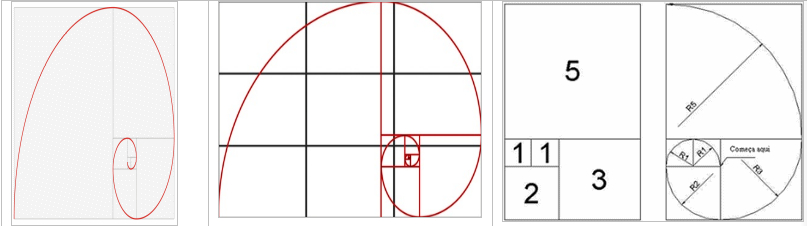
\includegraphics[width=95mm]{./imgs/fig7.jpg}
%\caption{III}
\end{figure}

O curioso desta curva é que ela, semelhante à projeção sobre os dois
eixos ortogonais de uma casca de caracol, os intercepta em quatro (e
mais infinitos) pontos, a saber: \versal{A, B, C, D}; a partir da origem \versal{O} são
vetores sucessivos que estão em progressão geométrica, ou seja, $\frac{\versal{OA}}{\versal{OB}}=\frac{\versal{OB}}{\versal{OC}}$ $\cdots{}$ m, qualquer que seja o valor de \emph{m}.

Basta observar um gráfico para verificar imediatamente que a espiral
logarítmica carrega dentro de si a imagem desse crescimento contínuo. A
este ponto surge naturalmente uma questão: qual é a ligação entre a
secção áurea, a mais perfeita figuração matemática da unidade do todo e
suas partes, e a espiral logarítmica, a mais perfeita figuração linear
do princípio de evolução regular em geral? Esta ligação existe: entre
todas as espirais logarítmicas possíveis, a única que não apenas traça o
princípio da evolução em geral, mas graças à qual se efetua o
crescimento real das manifestações da natureza é aquela onde as
relações: $\frac{\versal{OA}}{\versal{OB}}=\frac{\versal{OB}}{\versal{OC}}$ $\cdots{} =$
0,618; onde 0,618 é a medida do segmento áureo.

Esse exemplo, em si cativante, mostra como a ideia do orgânico,
coincidindo em todos seus traços particulares com o processo e os fatos
da natureza orgânica, se encarna nos traços e nas proporções do domínio
da matemática.

No quadro de Suríkov, representando a Boiárina Morózova, o `natural e o
belo' unem"-se justamente de acordo com o orgânico, no sentido que lhe é
conferido por Eisenstein; trata"-se apenas de procurar a secção áurea nas
proporções. Verificam"-se dois pontos dramáticos no quadro: de acordo com
os traços geométricos, ambos estão sobre dois eixos que passam a 0,618
de cada extremidade do quadro. Num deles está representada \emph{a
mão} da boiárina com os três dedos esticados com os quais era feito o
sinal da cruz, signo da controvérsia religiosa que o pintor quis
retratar no quadro. No outro, e muito sintomaticamente, está
representada \emph{a boca}, o lugar da `fala' da Boiárina, o lugar do
som das palavras daquela que os fanáticos daqueles tempos diziam ser
`uma leoa entre as ovelhas'.

\begin{figure}[!ht]
\centering
  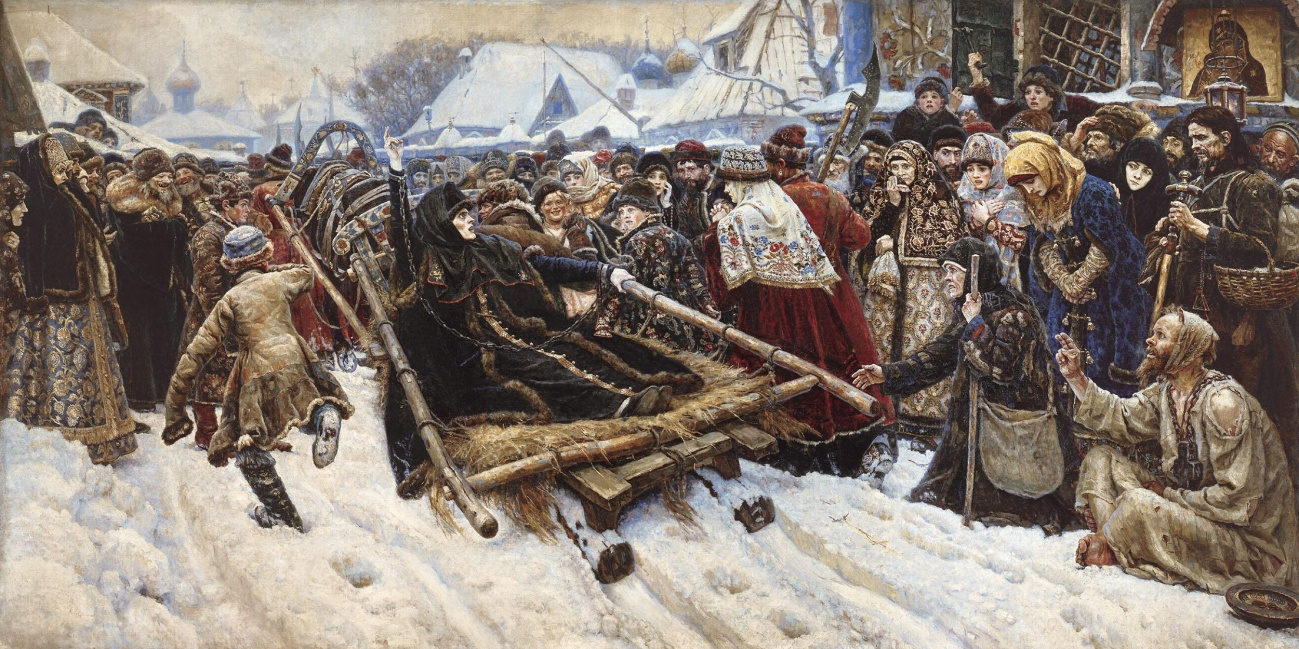
\includegraphics[width=95mm]{./imgs/fig8.jpg}
%\caption{III}
\end{figure}

Da mesma forma que ocorreu com o `orgânico', Eisenstein não pretende
aprofundar a natureza do `patético' enquanto tal. Interessa"-lhe examinar
a obra patética no plano de sua percepção pelo fruidor ou, mais
exatamente, no plano de sua ação sobre o fruidor. Partindo desses traços
particulares de sua ação, Eisenstein procurará definir os traços
específicos que deve possuir uma composição patética, exemplificando com
uma série de obras que vão do cinema às artes plásticas e literárias,
sobre as quais, obviamente, não nos deteremos aqui, e terminará com uma
série de conclusões de ordem geral.

Pode"-se dizer que a ação do patético de uma obra consiste em levar o
espectador a um estado de êxtase. \emph{Ex"-stasis}, significando,
literalmente, `sair de si mesmo', `estar fora de si', `sair do estado
habitual'. Quem estava sentado, levantou"-se, o imóvel pôs"-se em
movimento, o silente gritou, o seco tornou"-se úmido: todos são exemplos
da saída de um estado habitual. Há mais do que isso, porém, nessa
formulação. Sair de si mesmo não significa `sair para o nada'. Sair de
si mesmo deve significar necessariamente a passagem para alguma outra
coisa, de qualidade diferente e contrária ao que a precede. E mais, numa
estrutura patética, que provoca o efeito extático, todos os signos
distintivos devem ser submetidos à condição de `saírem de si' e à
passagem para uma outra qualidade. A estrutura desse tipo é o caso
limite da `saída de si mesmo'; todos os outros gêneros de composição de
arte podem ser considerados como derivados decrescentes deste caso
limite.

Eisenstein não aborda o problema do tema e do conteúdo. O que lhe
interessa são os meios que permitem realizar o patético na composição:
as particularidades dos procedimentos artísticos que aumentam a
`ressonância' do acontecimento, até o patético. Não há dúvida que, em
primeiro lugar, isso está ligado à atitude do autor para com o conteúdo.
Mas a composição, no sentido em que a entende Eisenstein, é precisamente
a estruturação que serve para traduzir a atitude do autor para com o
conteúdo, forçando o fruidor a adotar a mesma atitude para com esse
mesmo conteúdo.(A essa coincidência de atitudes entre autor/fruidor,
Liev Tolstói (1828--1910) chamou ``contágio'', em sua obra \emph{O que é
a arte}).

Seguindo as mesmas premissas que Eisenstein justificou quanto à questão
do orgânico, para que o fruidor saia de si mesmo, é preciso que lhe seja
dado, na obra, um `modelo' correspondente, segundo o qual
ele possa chegar ao estado desejado. O modelo mais simples --- os
`arquétipos' de tal comportamento por contágio --- ocorreria no cinema
ou no teatro, onde uma personagem `fora de si' levaria o espectador a
outro tanto. Lá, estrutura e representação seriam coincidentes. E o
objeto da representação --- o comportamento (ou atitude) de uma
personagem, ele mesmo se desenvolveria de acordo com a estrutura
`extática'.

As particularidades da palavra, contudo, são um pouco diferentes. No
momento em que se patetiza a palavra habitual, ela adquire um ritmo
nitidamente perceptível. Começa a assumir formas e figuras próprias da
linguagem poética, ocorrendo a passagem de uma qualidade a outra. Mais
complexo e mais eficaz é o contágio que atinge não somente a personagem
ou a palavra, mas a ambiência inteira. Um exemplo clássico é \emph{King
Lear}, de Shakespeare, onde o frenesi, ultrapassando os limites do
personagem, torna"-se o frenesi da natureza. Esta passagem para a
dimensão seguinte que provoca um efeito patético é, em geral, uma das
características de Shakespeare.

Uma vez esboçada a fórmula da construção das palavras patéticas e a
condição que determina o estado em que devem se encontrar ou revelar
todos os elementos da obra patética, para produzir o máximo de efeito, e
após tê"-los verificado numa série de exemplos de todo gênero, tempo e
lugar, Eisenstein coloca a seguinte questão: o que ocorre nas
circunstâncias da criação de uma obra patética, que fim persegue o
autor, em que condições psíquicas e psicológicas se cria uma obra dessa
natureza?

A resposta, sinteticamente, pode ser assim formulada: trata"-se de um
certo estado psíquico, mais do que psicológico, ao a qual o autor quer
ligar seu tema para produzir em seu público uma impressão marcante. Pode
fazê"-lo conscientemente ou chegar a isso independentemente de sua
vontade, por inspiração. E mais ainda: um pateticismo autêntico dá"-se
quando a consciência do querer e a espontaneidade da inspiração são
indissociáveis e seguem um mesmo processo de realização criadora e
quando esta união torna"-se a condição comum a todos os elementos da
obra.

Ao mesmo tempo que é indispensável a presença do ritmo autônomo,
vivificador e virtual, para que a obra exista, também a obsessão
temática do autor é premissa indispensável para todo `querer criativo'.
Um certo grau de obsessão pelo tema suscita este estado psíquico
`particular' que convoca as leis já citadas da percepção, da visão, do
enunciado e da representação para se fundirem em imagens vivas de todos
os dados do tema que aparecerão na obra acabada.

A um determinado grau do estado psíquico (`inspiração') sobrevém como
que um sentimento de comunhão com as leis do desenvolvimento dos
fenômenos da natureza, da mesma forma que a um determinado grau da
temperatura torna"-se possível a passagem do estado liquido ao gasoso, ou
a um determinado grau do estado das condições físicas, em energia.

Recapitulando o que foi dito, seria possível, \emph{grosso modo}, obter
as três fases seguintes do processo:

\begin{enumerate}
\def\labelenumi{\arabic{enumi})}
\item
  inspiração, por parte do autor, pelo objeto (ideia) do tema;
\item
  estado extático provocado pela intensidade da emoção inspirada para
`viver' o tema, estado este que se manifesta pela saída dos limites do
formal e do imaginado, na pura sensação de participação aos princípios e
aos processos do movimento da `ordem das coisas';
\item
  integração de seu tema e de sua obra a essa `ordem das coisas',
graças à recriação exata deste processo pelos meios da matéria de seu
tema.
\end{enumerate}

Exemplos do funcionamento destas fases, Eisenstein procura"-os, entre
outros, no domínio do êxtase religioso, em que, particularmente no
relato dos exercícios espirituais de Santo Inácio de Loyola, apesar dos
fins serem evidentemente outros, a `psicotécnica' parece ser bastante
semelhante.

Deixando de lado os exemplos, procuremos agora sintetizar os `meios'
propostos por Eisenstein para a obtenção do estado extático. Antes disso
porém, vamos acompanhá"-lo na acepção em que ele entende o termo
`comunhão'. Pelas descrições dos `extáticos' esta expressão evoca sempre
o estabelecimento de um contato, de um nexo, com algo que existe fora de
nós: `estar em comunhão de sentimentos com alguém', `sentir"-se em
comunhão com um grupo qualquer', `participar de um certo ato ritual',
`comunicar com um certo processo', etc. Para os extáticos religiosos, o
sentido do termo' extático' significa que comunicamo"-nos com um ente
sagrado, este entra em nós e nós entramos nele.

No caso que Eisenstein pretende considerar, a acepção do termo é outra.
Em primeiro lugar, nós não visamos nos comunicar com um ente, mas com a
percepção das leis da existência, da matéria, sentidas como um devir
perpétuo. Será que a comunhão, neste caso, implica estabelecer laços com
algo que existe fora de nós? Não, evidentemente, uma vez que nós também
somos parte dessa matéria. E, na medida em que somos uma sua expressão
particular, teoricamente, poderíamos descobrir e ressentir as leis do
movimento da matéria simplesmente `conhecendo"-nos a nós mesmos'. Seria
isso possível, sob a forma de uma representação objetivamente formulada
dessas leis? A resposta é novamente não. Isso porque uma `representação'
objetiva só é possível quando se pode representar objetivamente o
fenômeno, distanciando"-se dele e colocando"-o, por assim dizer, frente a
frente, de modo que qualquer coloração subjetiva seja eliminada. Ora, a
orientação para dentro de si próprio não pode nos proporcionar um
conhecimento objetivo, mas sim a sensação subjetiva de viver
emocionalmente aquelas leis. Resulta disso um estado extremamente
curiosos Por exemplo, um simples mortal `não encontra palavras' para
descrever o sentimento que o invade num arrebatamento amoroso, ou diante
de um pôr"-do"-sol. O artista, ao contrário, também é capaz de provar
intensamente o estado emocional subjetivo, mas além disso, é capaz de
transmiti"-lo numa forma objetiva, pela descrição, pela estrutura, pelas
imagens e pela lei reconstituída do processo da emoção. Qual é a
condição fundamental?

A condição fundamental é que, paralelamente a este conhecimento de si
mesmo, ele conheça os outros, ele tome consciência da existência
objetiva dos sentimentos nos outros.

Nesse processo o artista ocupa um ponto extremo: confrontado com os
sentimentos de outrem ele se vê separado e oposto --- ele se encontra nas
condições de um total e objetivo distanciamento. É então que a
comunidade das leis fundamentalmente idênticas e que regem identicamente
o `eu' e o `eles' dá a possibilidade de conhecer os outros através de
si, mas unicamente através dos outros, conhecer a si.

Na introspecção dos místicos, como se dizia, existe realmente a comunhão
com esta progressão do movimento da matéria. Porém, sem conhecimento
objetivo e unicamente no plano da emoção vivida.

Existem vários caminhos para atingir o estado de exaltação extática.
Três deles são particularmente eficazes, diz Eisentstein:

\begin{enumerate}
\def\labelenumi{\arabic{enumi})}
\item
  as formas mais grosseiras de êxtase --- como o êxtase físico dos
dervixes, xamãs, pajés etc. --- baseadas em princípios puramente físicos,
essencialmente ritmo"-motórios e uma ginástica especial;
\item
  os narcóticos e as drogas de diferentes espécies, sendo que, nesse
caso, o esquecimento individual faz com que o efeito seja quase que
imediatamente irreproduzível;
\item
  os `exercícios' espirituais' --- conseguidos com maior perfeição por
Santo Inácio de Loyola, por um sistema de ginástica psíquica particular,
repetindo no plano psíquico as manipulações físicas dos dervixes.
\end{enumerate}

Enfim, há uma infinidade de fenômenos ditos `subsensoriais' que agem
sobre nós, sem que estejam no campo de nossa consciência ou sequer no
âmbito de nossos sentidos. O que importa é que se saia, em certa medida,
do estado psíquico normalmente admitido. Que se afastem, em certa
medida, todas as fontes superestruturais das noções e dos conceitos
imaginados para que se atinja este estado original, sensorialmente
purificado, onde qualquer sistema elaborado de `exercícios' levará o
paciente ao êxtase. É a isso que está ligada a sensação de se dissolver
na natureza. A comunhão entende"-se como a percepção de um uníssono
universal, o fundir"-se no todo.

\chapter{\emph{Antologia do pensamento crítico russo (1802--1901)}}

O idioma russo provém do eslavo comum, língua que se separou do
indo"-europeu em tempos remotos e que deu origem ao russo antigo,
russo"-branco, ucraniano, polonês, tcheco, eslovaco, sérvio"-croato,
esloveno e ao búlgaro, com seu dialeto, o eslavo antigo.

O império Bizantino procurou estender, durante séculos, sua influência
política sobre as populações eslavas que catequizou (e alfabetizou, pois
não existia língua eslava escrita). No século \versal{IX}, os monges Cirilo e
Metódio, pertencentes a uma população eslava que habitava a região de
Salonica, na Grécia, tiveram o encargo de estabelecer o alfabeto --- que
viria a ser chamado cirílico --- e os fundamentos de uma língua na qual
seriam escritos os textos sagrados destinados a toda a população eslava.

Valeram"-se de sua própria língua, um dialeto do búlgaro antigo que
passou a ser conhecido como eslavo antigo ou eslavo eclesiástico ou,
ainda, eslavão. No final do século \versal{X}, quando a Rússia kievana se
converteu ao cristianismo ortodoxo, esse idioma se consagrou não apenas
como língua da Igreja, mas como língua literária do país. Deu"-se, então,
o seguinte paradoxo, o povo falava o russo (que só existia em forma
oral) e os livros eram
escritos em eslavo eclesiástico, não apenas os religiosos, mas a própria
grande epopeia russa (de autor desconhecido) o \emph{Dito do exército de
Ígor}, do século \versal{XII}.

Porém, o eslavo eclesiástico foi sofrendo a influência da língua falada
a ponto de a Igreja russa mandar proceder a uma revisão de todos os
livros eclesiásticos (século \versal{XIV}) para escoimá"-los de qualquer
influência estranha. A revisão repetiu"-se no século \versal{XVII}, quando a
Ucrânia foi incorporada à Rússia, influenciando o eslavo eclesiástico
russo com seu eslavo eclesiástico mais requintado e repassado de
polonismos. Contra a revisão dos livros eclesiásticos ordenada pelo
patriarca Nikon insurge"-se o arcipreste Avvakum que, em sua
autobiografia (\emph{Vida),} foi o primeiro escritor importante a
utilizar o russo, escrito em caracteres cirílicos, como língua literária.

Em 1755, ainda sob a influência do reinado do monarca esclarecido de Pedro, o
Grande(1678--1725), talvez o melhor dos czares, foi publicada a primeira
Gramática Russa, de Mikhail Lomonossov, que fundiu a língua popular à
eclesiástica, com alguma influência do grego e do latim,
 principalmente nos aspectos verbais e no uso das declinações. Sua
consolidação como língua literária deu"-se na geração de A. S. Púchkin (
1799--1837), o poeta nacional russo, que a tornou mais leve e mais
próxima da língua falada.

Essas informações, que remontam às aulas de Boris Schnaiderman, são
importantes para mostrar como é relativamente recente o fenômeno da
literatura russa, e para explicar porque as coletâneas de \emph{História
da literatura russa} costumem começar com excertos da \emph{Vida} (atribulada) do arcipreste Avvakum, e, tirante as crônicas e hagiografias
escritas em eslavão, passem diretamente à época de Púchkin. É
justamente com essa passagem que se inicia esta \emph{Antologia do
pensamento crítico russo}, organizada por Bruno Barretto Gomide para a Editora 34, cujo
primeiro texto, sobre a incipiência da literatura russa, (1802), de
Nikolai Karamzin, paradoxal e pessimista, mas cheio de expectativas,
prenuncia ``Da insignificância da literatura russa'', de 1834, do
próprio Aleksandr Púchkin que, por sinal, em seu famoso conto ``A dama
de espadas'' faz um dos protagonistas se queixar de que não há romances
russos para ler, mas apenas novelas copiadas de modelos do ocidente.

O período abarcado pela antologia, (1802--1901), foi escolhido, explica o
organizador, por alguns motivos fundamentais. Primeiro para mostrar como
``as idas e vindas entre texto crítico e texto literário produziram [e ainda produzem] uma dinâmica essencial para a vida intelectual
russa''; segundo, para ilustrar como a oposição \emph{ocidentalistas \versal{X}
eslavófilos} (estes, nacionalistas irredutíveis) que marcou, até a revolução
de 1917, as principais disputas da \emph{intelligentsia} russa, foi
particularmente intensa nesse século e, \emph{last but not least}, para
trazer ao conhecimento do leitor brasileiro, já relativamente
familiarizado com a literatura da Rússia, também alguns momentos
importantes de sua crítica, com o grande mérito de apresentá"-los sob
prismas diferentes. O primeiro exemplo que a antologia fornece é o da \emph{Primeira carta filosófica} (1836), de Piotr Tchaadáiev, onde a
expectativa de Karamzin e a sátira de Púchkin quanto à relação
Rússia"--Ocidente, levadas ao paroxismo pelo tom catastrófico, são
rebatidas por Aleksiéi Khomiakov, em suas ufanísticas \emph{Algumas
palavras sobre a `Carta filosófica'}.

Ora o mesmo autor apresenta facetas diferentes em análises diferentes (é o caso do já mencionado Karamzin, agora prefaciando otimisticamente a
\emph{História do Estado Russo} de 1818), ora se estabelece sobre a
mesma obra um diálogo de opiniões, geralmente contrastantes. É o caso da
recepção na Rússia da obra"-prima de Nikolai Gógol, \emph{As aventuras de Tchítchikov} ou \emph{Almas mortas}, por alguns considerada uma
farsa cruel e por outros uma epopéia, como faz Konstantin Aksákov em
\emph{Algumas palavras sobre o poema de Gógol} (1842). Ou seria, junto com
o \emph{Inspetor geral}, ``um desvelador das contradições históricas e
sociais da Rússia, com olhar crítico e ocidentalizante, como queria
Bielínski'', o crítico inclemente sobre o qual teremos ocasião de
voltar, que, em sua admirável \emph{Carta a Nikolai Vassílievitch Gógol} (1847) enaltece"-lhe as primeiras obras mas vergasta"-lhe as últimas (no
final de sua vida Gógol tornou"-se cada vez mais religiosamente exaltado
e panfletário). ``Segundo o senhor'', escreve Bielínski, ``o povo russo
é o mais religioso do mundo. Mentira! A base do sentimento religioso é a
piedade, a devoção, o temor a Deus. O russo pronuncia o nome de Deus
coçando o traseiro. (\ldots{}) Observe com cuidado e o senhor verá que este é
um povo profundamente ateu, por sua natureza. Há nele ainda muita
crendice, mas não há vestígio de sentimento religioso. (\ldots{}) O povo
russo não é assim: a exaltação mística não está de modo algum em sua
natureza; ele tem bom senso, lucidez e espírito confiante demais para
isso, e talvez aí, justamente, se encerre a grandeza de seu destino
histórico no futuro'' (p. 151--2).

Além das cartas, há alguns discursos notáveis nessa antologia. À parte
os do filósofo Vladímir Solovióv que vê na Igreja o ideal social de
Dostoiévski (1881--1883), ideal esse contrastando com \emph{O talento
cruel} (1882), quase psicanalítico, que o publicista Nikolai Mikhailóvski reconhece
ao escritor, há o famoso discurso do próprio Dostoiévski por ocasião da
inauguração de uma estátua a Púchkin (1880), onde, após um brilhante
apanhado da obra do homenageado chega à proposta de uma comunhão
universal: ``Sim, é incontestável que a vocação do homem russo é unir a
Europa e o mundo todo. Ser um verdadeiro russo, ser russo o suficiente,
pode significar e significa apenas (\ldots{}) tornar"-se irmão de todos os
homens, um homem universal, por assim dizer. Ah, todo esse nosso
eslavofilismo e ocidentalismo é apenas um grande equívoco, embora
historicamente necessário'' (p. 422).

Historicamente necessário será, de acordo com Gueórgui Plekhanov em seu
discurso sobre a obra e o pensamento de Vissarion G. Bielínski (1898),
talvez o mais importante do livro, aquilo que curiosamente (e
profeticamente) o ocidentalista socialista Bielínski, que tanto
exaltara \emph{Pobre gente} de Dostoiévski, chegou a propor quase como
testamento. ``O meu amigo crente'', escreve Bielínski numa carta a
Ánnenkov de fevereiro de 1848, talvez referindo"-se a Bakúnin, ``e os
nossos eslavófilos, ajudaram"-me muito a abandonar a crença mística no
povo. Onde e quando o próprio povo se libertou? Sempre tudo se fez pela
personalidade. Quando eu, em nossas discussões sobre a burguesia,
chamei"-lhe conservador, fui um asno ao quadrado, enquanto o senhor foi
um homem inteligente. Todo o porvir da França está nas mãos da
burguesia, todo o progresso depende apenas dela, enquanto o povo possa
talvez desempenhar algum papel passivo e acessório de tempos em tempos.
Quando eu, diante de meu amigo crente, disse que agora a Rússia precisa
de um novo Pedro, o Grande, ele atacou minha ideia como se fosse uma
heresia, dizendo que o próprio povo deve fazer tudo para si próprio. Que
pensamento ingênuo, arcádico!'' Como é que essa convicção surgiu em
nosso crítico? Pergunta"-se Plekhanov no decorrer de sua
análise, talvez a mais importante do livro.

Quanto aos artistas falando da arte de escrever, são imperdíveis o
ensaio de Toltsói de 1859, sobre os contos de suas \emph{Cartilhas} (Ed.
Ateliê e Cosac\&Naify), recontados pelos escolares de Iásnaia Poliana; o
de Gógol \emph{Algumas palavras sobre Púchkin}, de 1835, e o de Dobroliúbov
de 1859, sobre o fenômeno do ``oblomovismo'', já conhecido pelo público
brasileiro que tenha lido \emph{Oblómov}, a obra"-prima de Gontcharóv
(Cosac\&Naify).

Finalmente, dando as primeiras respostas às indagações de Ánnenkov (mas
não só dele) \emph{Sobre o significado das obras de artes para a sociedade}
(1856), temos o ensaio \emph{Sobre o método e as tarefas da história da
literatura como ciência} (1870), do grande linguista Aleksandr
Vesselóvski, o antepassado dos formalistas russos, que anuncia as novas
teorias. Mas já estamos no século \versal{XX}.

\chapter*{Formalismo e poesia: um balanço da contribuição dos formalistas russos numa
área específica da investigação literária}

\addcontentsline{toc}{chapter}{Formalismo e poesia}
\hedramarkboth{Formalismo e poesia}{}


\section{1}

O que até hoje surpreende no Formalismo Russo quando se tenta fazer um
balanço de sua contribuição nos diferentes setores da indagação
literária --- e particularmente no campo que escolhemos, o da poesia ---,
é sua incrível atualidade. Desde seu surgimento em 1915--1916 passaram"-se
quase cem anos e no entanto seus achados continuam válidos e, apesar de
pressentidos, ainda não de todo explorados. Ainda no século \versal{XIX} Aleksandr
Potebniá, um de seus mais ilustres precursores, seguindo as pegadas de
Wilhelm von Humboldt, declarara que a poesia é um dos dois modos
fundamentais da apreensão do real, ou seja, é aquele do conhecimento
``pela mediação da palavra''.

\section{2}

E mais --- diz ele ---, pelo fato de a linguagem tender a libertar"-se do
jugo do pensamento e lutar pela suprema autonomia da palavra é que a
poesia, ``a aspiração ideal da linguagem'', encontra maiores
possibilidades de realização. A diferença entre as duas apreensões do
real, a da ciência e a da poesia, não está nos fins que elas perseguem,
visto que ambas visam à ordenação da experiência, mas enquanto a ciência
se ocuparia com material homogêneo, a poesia dá uma resposta específica
a um problema específico.

\section{3}

A ênfase dada à metáfora não era, é claro, novidade em Potebniá
(\emph{Iz Leksi po Teorii Slovesnosti. Kharkov}, 1884, p. 99). Já
Aristóteles, na Poética, via no ``domínio da metáfora'' a prova suprema
da capacidade de um poeta, prova essa que depois se tornou a pedra de
toque da teoria romântica da poesia. Mas se a concepção da poesia como
discurso autônomo será assumida pelo Formalismo como um de seus
pontos"-chave, a concepção potebniana da imagem vista como procedimento
explicativo, como atalho mental que ``substitui uma massa heterogênea de
imagens por pequenas unidades intelectuais'', virá a ser controvertida
pelos formalistas russos e substituída por outra praticamente oposta: a
função da imagem não consiste em tornar mais acessível o inusitado, mas
sim em tornar estranho o habitual, apresentando"-o sob uma nova luz.

\section{4}

Enquanto Potebniá indagava sobre a dinâmica semântica da linguagem
poética, outro grande precursor, o estudioso russo Aleksandr Vesselóvski
(1838--1906), dirigia seus esforços no sentido da fundação de uma
História da Literatura como disciplina em si, com fins e métodos bem
definidos. Insistia, como ponto de partida, em tentar encontrar um
resposta para a questão ``o que é literatura?'' e, apesar de não ter
chegado àquela definição de ``literaturidade'' que Jakobson proporia alguns
anos mais tarde, V. Vesselóvski, em sua \emph{Poética histórica}, se
detém sobre a questão crucial para os formalistas dos procedimentos
artísticos e dos gêneros literários, focalizando na poesia mais que o
poeta e os processos psíquicos que o acompanham, a estrutura objetiva da obra literária.

\section{5}

Se os formalistas, por sua vez, se recusaram a explicar a literatura
baseando"-se nos processos psicológicos, sociológicos etc. (não
esqueçamos, porém, a questão da inserção das diferentes séries e a da
evolução literária para as quais, passado o momento polêmico, sempre
estiveram atentos), eles também se mostraram arredios quanto a procurar
a ``literaturidade'' no nível da experiência contida na obra de arte
literária ou a aceitar a opinião corrente de que o objetivo privilegiado
da poesia seriam as emoções, enquanto o da prosa seriam as ideias.

``Não há motivos mais poéticos que outros, e hoje tudo pode servir de
material para a poesia'', escrevia Roman Jakobson em ``O que é
poesia?'', enquanto Iúri Tyniánov, acentuando a fluidez dos limites
entre ficção e realidade, insistia no fato que a diferença entre
literatura e não"-literatura devia ser procurada não no tema, mas na
maneira pela qual a realidade é apresentada. A mesma questão foi
colocada, dentro da literatura, para se estudarem as diferenças entre
prosa e poesia.

\section{6}

Apesar de Jakobson ter sustentado numa série de trabalhos a conhecida
tese de que a poesia tende para a metáfora (associação por semelhança)
enquanto a prosa tende para a metonímia (associação por contiguidade), e
que a função poética da linguagem implica a ênfase na expressão da mensagem, está
claro que tanto a metáfora quanto a linguagem poética não são o fator
construtivo da poesia. (cf. Roman Jakobson. \emph{Noviéchaia Rússkaia
Poésia.} Praga, 1921, p. 11. E também, em português, Roman Jakobson,
\emph{Linguística e Comunicação}. São Paulo, Cultrix, 1969.)

\section{7}

Entre outros livros valiosos sobre o assunto, existe um livrinho de
Tyniánov que originariamente tem o título de \emph{O problema da
linguagem em verso} (Existe uma tradução em
português pela Editora Tempo Brasileiro), onde é dada uma explicação, às
vezes complexa, mas sempre extremamente convincente de como funciona a
poesia. É dele que vamos falar um pouco agora. Tomemos como ponto de
partida a constatação de Carlos Drummond de Andrade, de que o ritmo é o
verdadeiro fator constitutivo da poesia (inclusive, no caso, do próprio
verso livre):

\begin{quote} 
(\ldots{}) Então rasguei aquilo e parti impávido para a poesia
de verso livre --- na ilusão de que era mesmo livre. Não há verso livre.
O verso obedece às leis do ritmo. O verso, para ser verso, tem que ter
uma estrutura musical, uma cadência. Não importa que você faça quatorze
versos de dez sílabas cada um, divididos em dois quartetos e dois
tercetos, ou faça como os ingleses, que usam outra divisão. O verso pode
ter dez sílabas na primeira linha, quatro na segunda, seis na terceira.
É preciso que essas linhas reunidas formem um conjunto rítmico. É como a
música moderna, feita mais de dissonâncias do que de consonâncias. Isso
facilitava muito meu trabalho (\ldots{}).\endnote{(C. D. A. em entrevista ao
``Folhetim'' de 03/06/1984).}
\end{quote}

Vejamos qual será a justificativa que disso dá Tyniánov em seu livro.

\section{8}

O que acontece se transcrevermos em prosa o verso livre?

Podem se dar duas ocorrências: 1ª --- as divisões do verso não coincidem
com as divisões sintáticas, devido à disposição gráfica. Bem, ao passar
para a prosa as divisões desaparecerão. De tal modo ficará destruída a
unidade da série poética e mais, juntamente com ela, será destruído
outro elemento indicativo, ou seja, precisamente aqueles laços estritos
graças aos quais a unidade poética consegue manter, amarradas em si
mesmas, as palavras: o caráter compacto da série poética. O ritmo no
verso é indicativo justamente pela unidade e pela compressão da série
do material do discurso. Esse é o motivo pelo qual o conteúdo
quantitativo da série poética é limitado, e, quando o verso é longo
demais, ou ele se divide em outras unidades, ou perde a noção de seus
limites. Em ambos os casos deixa de ser unidade. Os dois elementos
referidos, a unidade e a compressão da série poética, dão lugar a um
terceiro traço distintivo que é a dinamização do material do discurso. A
série discursiva na poesia é mais compacta e mais amarrada do que no
discurso comum e evidencia infalivelmente a unidade do verso. Nas formas
estabelecidas de versificação a unidade de medida será menor que o verso
(pé ou sílaba) enquanto que, na versificação livre, cada verso será
assumido como norma. No caso do verso regular temos então uma
dinamização de palavras: cada palavra é objeto, ao mesmo tempo, de
várias categorias de discurso (é palavra discursiva, é palavra métrica).

\section{9}

No caso do verso livre tem"-se frequentemente a dinamização de grupos,
sendo que o grupo pode consistir numa única palavra. Assim, enquanto a
unidade e a compressão da série poética impõem uma nova ordem às
articulações e aos nexos sintáticos"-semânticos (no caso em que a
série poética coincida com a unidade gramatical, elas aprofundam e
sublinham os momentos dos nexos e das articulações sintático"-semânticas), a dinamização do material do discurso leva a uma nítida
separação entre palavra poética e palavra comum. O sistema de interação
entre as tendências da série poética e do conjunto gramatical da palavra
métrica e da palavra discursiva, assume um papel decisivo. A palavra
torna"-se um compromisso, uma resultante das duas séries, assim como a
frase. A palavra torna"-se dificultada e o processo do discurso torna"-se
secundário. Se, conforme dizíamos, transformarmos em prosa o verso livre
em que a série poética não coincida com a série sintática, estaremos
violando a unidade e o caráter compacto da série poética, privando"-a de
sua capacidade de dinamizar o discurso: emergirá o princípio construtivo
da prosa e em lugar dos nexos e das articulações do verso, passarão a
atuar os nexos e as articulações de natureza sintático"-semântica.

\section{10}

O que acontece, então, quando se passa para a prosa o verso livre
em que a série coincide com a unidade (ou o conjunto) gramatical? Resumindo: a
unidade da série poética é destruída, passando a coincidir com a unidade
sintática; o momento de compactude da série poética decai, permanecendo
uma ligação marcada entre os membros da unidade sintática, e a poesia
acaba por desfazer"-se por lhe faltar um de seus traços distintivos: o
momento da dinamização do discurso. A série poética, mesmo não perdendo
de todo suas características, não será mais poética; no desenvolvimento
do material não mais se notará a medida do verso, a sua unidade, e
juntamente com ela não terá havido a dinamização da palavra e de seus
agrupamentos, resultando isso tudo no decaimento do caráter secundário
da palavra no verso. O princípio construtivo de qualquer série tem uma
força assimilativa e deformante em relação aos fenômenos de uma outra
série. O segredo está na subordinação de um momento a outro, e na
poesia, contrariamente à prosa, a influência deformante deve ser
procurada no ritmo, juntamente com o princípio de associação simultânea
dos elementos do discurso.

\section{11}

Veja"-se como Manuel Bandeira pressente esse ``segredo'' numa das
epígrafes de ``A Música da Poesia'': ``Cedo compreendi que o bom fraseado não é
fraseado redondo, mas aquele em que cada palavra tem uma função precisa,
de caráter intelectivo ou puramente musical, e não serve senão à palavra
cujos fonemas fazem vibrar cada parcela da frase por suas ressonâncias
anteriores e posteriores''. (1966, p. 45).

\section{12}

Além do problema do ritmo, visto como fator construtivo da poesia, o
objeto do livro de Tyniánov é o material de que a poesia e feita e, mais
particularmente, ``o sentido da palavra no verso''. Essa questão não
menos complexa, por ele submetida a um exame rigoroso, leva"-o a
``achados'' extremamente esclarecedores. Ele utiliza como exemplo uma
série de poemas russos, mas podemos novamente recorrer a Drummond, cuja
milagrosa ``Procura da Poesia'' os sintetiza quase todos. Somente
sentimos, devido à sua extensão, poder reproduzir apenas uma parte dessa
procura:

\begin{verse}
(\ldots{}) A poesia (não tires poesia das coisas) \\
elide sujeito e objeto. \\[8pt]
Não dramatizes, não invoques, \\
não indagues. Não percas tempo em mentir. \\
Não te aborreças. \\
Teu iate de marfim, teu sapato de diamante, \\
vossas mazurcas e abusões, vossos \qb{}esqueletos de família \\
desaparecem na curva do tempo, é algo \qb{}imprestável. \\[8pt]
(\ldots{}) Penetra surdamente no reino das \qb{}palavras. \\
Lá estão os poemas que esperam ser escritos. \\
Estão paralisados, mas não há desespero, \\
há calma e frescura na superfície intata. \\
Ei-los sós e mudos, em estado de dicionário. \\
Convive com teus poemas, antes de \qb{}escrevê"-los. \\
Tem paciência, se obscuros. Calma, se te \qb{}provocam. \\
Espera que cada um se realize e consume \\
com seu poder de palavra \\
e seu poder de silêncio. \\
Não forces o poema a desprender-se \qb{}do limbo. \\
Não colhas no chão o poema que se perdeu. \\
Não adules o poema. Aceita-o \\
como ele aceitará sua forma definitiva e \qb{}concentrada no espaço. \\[8pt]
Chega mais perto e contempla as palavras. \\
Cada uma \\
tem mil faces secretas sob a face neutra \\
e te pergunta, sem interesse pela resposta, \\
pobre ou terrível, que lhe deres: \\
Trouxeste a chave? \\[8pt]
Repara: \\
ermas de melodia e conceito, \\
elas se refugiaram na noite, as palavras. \\
Ainda úmidas e impregnadas de sono, \\
rolam num rio difícil e se transformam \qb{}em desprezo.
\end{verse}

\section{13}

Afora a questão do ritmo e a unidade do verso, coincidindo e não
coincidindocom a unidade lógico"-sintática, que é visível nas várias
estrofes do poema, aí estão, na ordem em que foram mencionados, a imagem
tornando estranho o habitual (``Teu iate de marfim, teu sapato de
diamante'') e funcionando como metáfora e metonímia ao mesmo tempo. Lá
está, em todos os \emph{não}, a afirmação da literaturidade e a
suspensão (``não te aborreças''), das outras séries. Fica quase
didaticamente explicada, no poema, a ausência de motivos privilegiados
(``não tires poesia das coisas'') e a soberania da palavra (``Penetra
surdamente no reino das palavras''). Lá estão a forma dificultada
(``rolam num rio difícil'') e a ``forma definitiva e concentrada''.
Existem, porém, dois elementos nesse poema que gostaríamos de analisar
um pouco mais detidamente, pois se prendem a dois conceitos que Tyniánov
desenvolveu de modo bastante fecundo na segunda parte de seu livro. O primeiro
deles é aquele ``poder de palavra'' contraposto ao ``poder de silêncio''
de Drummond, que Tyniánov chama de ``equivalentes do texto''. Claro que
o alcance desse silêncio quase metafísico de Drummond é mais imediato em
Tyniánov, mas vejamos o que este diz a respeito.

\section{14}

Para Tyniánov, a ideia do verso como dado sonoro se encontra, antes de
mais nada, diante da constatação de que alguns fatos essenciais da
poesia não se esgotam na manifestação acústica do verso, pelo contrário,
a ela se opõem. Entre eles estão os equivalentes de texto, ou seja,
todos os elementos extra"-verbais que, de um modo ou de outro, o
substituem: certas omissões parciais, certas substituições parciais por
elementos gráficos e outros. O que é importante é verificar que o
fenômeno dos equivalentes (de metro, de verso, de estrofe etc.) não
implica atenuação ou relaxamento, mas pelo contrário, implica pressão,
tensão de elementos dinâmicos que não devem ser confundidos com a pausa,
elemento homogêneo do discurso que ocupa um determinado lugar.

\section{15}

O último e mais crucial elemento que vamos abordar se prende mais
literalmente ao sentido da palavra poética e vem introduzido pela
penúltima estrofe do poema acima citado de Drummond:

\begin{verse}
Chega mais perto e contempla as palavras. \\
Cada uma \\
tem mil faces secretas sob a face neutra \\
e te pergunta, sem interesse pela resposta, \\
pobre ou terrível, que lhe deres: \\
Trouxeste a chave?
\end{verse}

Pois bem, essas mil faces secretas que se escondem sob a face da
palavra são para Tyniánov os indícios de significado. Sem pretender
desenvolvê"-los, vamos apenas resumi"-los utilizando, em alguns casos, os
próprios exemplos de Tyniánov. Apagando"-se o significado mais habitual
da palavra (ou seja, o indício fundamental de seu significado) nela se
manifesta mais fortemente seu matiz léxico, que é um indício secundário
permanente de seu significado. Os indícios lexicais mais fortes aparecem
nas palavras que não têm indícios fundamentais de significado: nomes
próprios, barbarismos ou palavras simplesmente desconhecidas para o
remetente. Curioso é um exemplo retirado de ``Os camponeses'', de
Tchekhov:

\begin{quote}
Sacha levantou as sobrancelhas e começou alto, em tom de ladainha: ---
Partidos que foram, um anjo do Senhor apareceu em sonho a José dizendo:
``Levanta"-te, pega o Menino e sua Mãe\ldots{}'' ``O Menino e sua Mãe'' repetiu
Olga corando de comoção. ``E foge para o Egito. Nesse ínterim\ldots{}'' à
palavra `Nesse ínterim', Olga não se aguentou e desatou a chorar.
\end{quote}

Este exemplo é um caso limite. Em poesia os indícios lexicais não
eliminam os indícios fundamentais de significado, mas criam o assim
chamado tom lexical, o qual, unido aos indícios flutuantes de
significado (diferentes em cada caso), constitui o significado da
palavra poética dentro de um dado contexto. A palavra não existe
isolada, diz o autor. Mesmo que ela seja proferida isoladamente, fora de
qualquer frase, é inevitável que provoque no ouvinte séries
associativas. Os significados ocasionais que podem ser associados à
palavra passam a funcionar como indícios secundários de significado que
operam sobre o indício fundamental, dando origem a uma série de
alterações. Assim, no trecho final de um poema de Marina Tsvetáieva
(1917) traduzido do russo por Elsa Triolet, temos as duas (ou mais) acepções da
palavra ``brumas'' (brumes):

\begin{verse}
\ldots{} Ainsi, debout, mains dans les poches, \\
Avec l'ocean entre nous\ldots{} \\
La ville dans les brumes, \\
Brumes anciennes de l'amour.
\end{verse}

\section{16}

Ou então outro exemplo, ainda da mesma autora: ``Sobre os negros contornos
do cabo/A lua --- armadura de cavaleiro''.

Observa"-se uma espécie de irradiação do significado dos elementos
materiais e formais que constituem o signo /lua/ e uma tendência a se
orientarem para a determinação de um conceito. A matização da palavra
``lua'' não provém da anulação de seu indício fundamental, mas de sua
permanência. Estamos diante de dois planos semânticos distintos, cada um
dos quais tem seus indícios fundamentais e se equilibra com o plano
paralelo. A flutuação dos dois planos semânticos pode ocasionar o
obscurecimento parcial do indício fundamental, dando origem ao fenômeno
que estamos acostumados a chamar de metáfora. Entre os indícios
secundários manifestam"-se alguns que, por sua instabilidade, foram
chamados de indícios flutuantes. De uma maneira geral, eles são frutos
da ambiguidade entendida no sentido de William Empson (\emph{7 types of ambiguity}. New York: New Direction, 1966): ``Any
verbal nuance which gives room for alternative reactions to the same
piece of language''.

\section{17}

Esses indícios flutuantes podem estar ligados a fenômenos de som, como
no ``Conto do czar Saltan'' de Púchkin, agora, necessariamente, em
russo:

\begin{verse}
\emph{I v sumú evó pustúiu} \\
(E em sua bolsa vazia) \\[8pt]

\emph{Súiut grámotu drugúiu} \\
(Colocam outra ordem).
\end{verse}

Pode"-se notar que o primeiro verso corresponde ao segundo com o grupo
\emph{su (sumú -- súiut}) e uma sua repetição parcial é encontrada na
palavra \emph{pustúiu}. A extraordinária força expressiva do verso
depende aqui da labialização do som \emph{u}; a repetição deste som torna a
articulação ainda mais forte na medida em que estas repetições dão o som
não de forma monótona, mas pela alternância de seus diferentes matizes,
o que produz uma impressão de articulação prolongada. Com isso os
significantes das palavras passam a ser bastante deformados --- é como se
o indicio fundamental da palavra \emph{sumú} (bolsa), ligada sintática e
foneticamente com \emph{pustúiu} (vazia), por sua vez regressivamente
ligada com \emph{súiut,} retrocedesse diante de indícios flutuantes já
perceptíveis. Assim, aqui agem não apenas o matiz semântico geral da
série, mas também um deslocamento do significado da palavra, devido à
sua estreita ligação rítmica com as outras palavras.

\section{18}

Um exemplo, entre muitos, que não poderia faltar, apresenta os indícios
flutuantes ligados aos fenômenos de tom, que Tyniánov foi procurar em
Montesquieu:

\begin{verse}
\emph{Centrenthus, Areca, Tegestas, Luscaris} \\
\emph{Messanbrianthemum et Strutiopheris} \\
\emph{Arthuriam, Raphis, Arecas et Limanthe\ldots{}}\endnote{MONTESQUIEU
  apud TYNIÁNOV, Iúri. \emph{O problema da linguagem poética II}. Rio de
  Janeiro: Tempo brasileiro. 1975, p. 68}
\end{verse}

Temos aqui, ao lado de um tom lexical estável, dado pelo emprego de
nomes próprios, também o surgimento de um \emph{tom transmental} e, com
a intensificação dos indícios flutuantes, a criação de uma semântica
imaginária, tão cara aos futuristas russos, que com sua obra fornecem um
campo inesgotável para a prática e a comprovação das teorias
formalistas.

Para encerrar, eis como Tyniánov interpreta a ``Encantação Pelo Riso''
do Futurista Velimir Khlébnikov:

\begin{verse}
Ride, ridentes! \\
Derride, derridentes! \\
Risonhai aos risos, rimente risandai! \\
Derride sorrimente! \\
Risos sobrerristos -- risadas de sorrideiros \qb{}risones! \\
Hílare esrir, risos de sobrerridores riseiros! \\
Sorrisonhos, risonhos, \\
Sorride, ridiculai, risando, risantes, \\
Hilariando, riando, \\
Ride, ridentes! \\
Derride, derridentes!\endnote{KHLÉBNIKOV, Velímir. ``Encantação pelo
  riso'', In:\emph{Poesia Russa Moderna.}(tradução de Haroldo de
  Campos). Rio de Janeiro. Civilização Brasileira, 1968.}
\end{verse}

Vê"-se aqui a intensificação do significado geral e o papel semântico
considerável de cada palavra isolada. Com isso, pela importância do
quadro sintático nesta diferenciação de palavras fundadas sobre uma
parte objetiva comum, assumem importância também os próprios elementos
formais das palavras, cuja semântica emerge tanto mais forte quanto mais
a parte objetiva das palavras coincide. Esta coincidência impõe à parte
objetiva individual de cada palavra uma relativa atenuação: seu
significado é absorvido pelo significado geral e toda ênfase vai para as
variantes da parte objetiva.


\chapter{Formalismo russo, uma revisão e uma atualização}

Quando saiu em francês a reunião de textos dos formalistas russos de
Tzvetan Todorov (\emph{Seuil}, 1965) \emph{Textos dos formalistas
russos}, visto que a edição brasileira da Globo, um pouco modificada,
\emph{Textos dos formalistas russos} só sairia em 1970, a primeira
disciplina que frequentei no Curso de Pós"-graduação em Teoria Literária
e Literatura Comparada, ministrada pelo Prof. Antonio Candido, propunha
justamente, como estudo principal, a análise e a discussão daqueles
textos. Recordo com que deslumbramento assistíamos ao seminário de
``Como foi feito \emph{O capote} de Gógol'' (que a colega que o
apresentou chamava com desenvoltura o \emph{mantô}) aquele pobre Akáki
Akákievitch que eu teimava em associar a um cômico italiano --- Renato
Raschel, se não me engano --- que o havia interpretado num filme
tocantíssimo no Cine Coral, (hoje desaparecido --- quem diria?) fazendo num rompante inesperado toda aquela declamação patética, que na
verdade era o ``gesto fônico'' que se interpunha à ``narração cômica''!
E a semântica fônica do conto era estudada em termos de \emph{skaz,
discurso direto, discurso indireto, diálogo} etc. em moldes bakhtinianos
\emph{avant la lettre}. Isso, em se tratando de prosa, foi apenas o começo.
Depois do \emph{mantô} de Eikhenbaum viria ``A temática'' de
Tomachévski, com a \emph{fábula} e o \emph{siujet}, os motivos livres e
suas funções, para cuja diferenciação Boris Eichenbaum forjou o conceito
de \emph{dominante}, a motivação dos procedimentos, o estranhamento ou
singularização, a ``Evolução literária'' de Tynianov etc. etc. As
\emph{funções} de Propp nos contos maravilhosos só vinham prenunciadas
em seu ensaio sobre as ``Transformações dos contos maravilhosos''
(``fantásticos'', erroneamente traduzido, na ed. Da Globo): seu livro
\emph{Morfologia do conto maravilhoso}, com a resposta a
Lévi"-Strauss\endnote{No tocante à polemica Lévi"-Strauss/Propp que, na
  época, só saíra na tradução italiana do livro de Propp
  \emph{Morfologia do conto maravilhoso}, e que em 1984 saiu também na
  versão brasileira do livro na tradução de Iasna P. Sarhan (Editora
  Foresce Universitária), vale a pena
  resumir seus aspectos principais pois é o exemplo que daremos de como
  e por que certos equívocos em relação ao formalismo russo acabaram se
  generalizando e se perpetuando. Lévi"-Strauss defendia a tese de que a
  noção de forma e a de estrutura não são equivalentes: ``A forma se
  define por oposição a uma matéria que lhe é estranha, enquanto que a
  estrutura não tem conteúdo distinto; ela é o próprio conteúdo
  apreendido numa organização lógica concebida como propriedade do
  real'' (p. 182). Com isso, e acusando Propp de ter começado seu estudo
  pela análise morfológica que, insatisfeito com os resultados, teria
  abandonado mais tarde pela pesquisa histórica e comparativa,
  Lévi"-Strauss queria chegar a demonstrar que o modelo ``formalista'' de
  Propp e o estruturalista eram diferentes e visavam resultados
  diferentes. Propp responde que a análise empreendida em
  \emph{Morfologia} era apenas o começo de uma pesquisa mais ampla que
  envolveria discutir a vocação histórica do gênero ``conto
  maravilhoso'' (Cf., entre outros, o volumoso livro de Propp que viria
  em seguida\emph{, Raízes históricas do conto}) e que a pesquisa
  histórica seria inviável se não se procedesse, previamente, a uma
  definição de seu estudo a partir do levantamento de seus elementos
  constituintes e que ele, Propp, jamais poderia propor uma separação
  entre forma e conteúdo: ``Como já dissemos, costuma definir"-se como
  formalista o estudo da forma desligada do conteúdo. Devo reconhecer
  que não compreendo o que isso significa --- que de fato não sei como
  entendê"-lo, nem como aplicá"-lo ao material em estudo. Talvez o compreendesse se soubesse
  onde procurar a forma, na obra de arte e onde o conteúdo. Sobre a
  forma e o conteúdo em geral, como categorias filosóficas, pode"-se
  discutir o quanto se quiser, mas estas discussões serão estéreis se,
  desde o inicio o objeto da discussão forem as categorias de forma em
  geral e de conteúdo em geral, sem referencia ao material concreto que
  se tem em vista, dentro de sua infindável multiplicidade. Para a
  estética popular, o enredo como tal constitui o conteúdo da obra.
  (\ldots{}) Todo interesse reside naquilo que aconteceu. Coloquemo"-nos,
  por um momento, dentro do ponto de vista popular (que, por sinal, é
  bastante sábio). Se o enredo pode ser denominado conteúdo, o mesmo não
  acontece em absoluto com a composição. Concluímos então que a
  composição se relaciona com o campo da forma, na obra em prosa. Desse ponto de vista,
  numa só forma podem ser incluídos vários conteúdos. Só que --- conforme
  tentamos demonstrar anteriormente ---, composição e enredo são
  inseparáveis. O enredo não pode subsistir fora da composição e esta
  fora do enredo. Baseados em nosso material chegamos a reafirmar a
  conhecida verdade que forma e conteúdo são inseparáveis'' (pp. 21,
  22).

  Para Lévi"-Strauss, a ``morfologia'' só sabe lidar com os dados
  invariáveis, uma vez que ela se torna método eficaz ao ignorar o
  conteúdo histórico dos contos analisados. A morfologia, em outras
  palavras, seria um método que se afastaria do concreto, enquanto o
  estruturalismo propunha
  um retorno ao concreto. Lévi"-Strauss ainda diz que Propp teria
  escolhido como ponto de partida um material narrativo inadequado, ao
  restringir"-se aos contos maravilhosos russos, pois o modelo proppiano
  de 31 funções e 7 protagonistas não seria exclusivo deles, mas se
  prestaria melhor como matriz de narrativas míticas. Ora, diz Propp,
  se Lévi"-Strauss entreviu nessa extrapolação a universalidade do modelo
  construído e/ou possibilidades futuras de operar analiticamente com
  ele com base em material mais abrangente, deveria Lévi"-Strauss, por
  coerência, ter reconhecido o mérito e o alcance da \emph{Morfologia}.
  O projeto de Lévi"-Strauss era, já na época da divulgação no Ocidente
  do livro de Propp (final dos anos 50), analisar os relatos míticos
  para desvendar"-lhes não a estrutura (o modelo narrativo), mas as leis
  lógicas que, agindo inconscientemente, configurariam o modelo
  narrativo. O campo de interesse de Lévi"-Strauss estava
  centrado, conforme se vê, no ``pensamento mítico'', um substrato
  lógico que estaria por trás dos arquétipos, que a ``morfologia'' lendo
  os mitos poderia elaborar. Ora, esse objetivo não era visado pelo
  folclorista russo, que só queria estudar o gênero \emph{conto
  maravilhoso} e não a relação mito/conto, embora seu método pudesse
  aduzir elementos que, reformulados, poderiam servir de ``chave'' de
  acesso ao pensamento mítico.} seria um capítulo à parte, um curso à
parte, já agora, ministrado pelo Prof. Boris, como também seriam cursos
à parte, em se tratando de poesia, \emph{O problema da palavra poética}
de I. Tynianov\endnote{Como demos um exemplo sintético de polemica com
  o formalismo russo, daremos agora um exemplo da marcha de uma de suas
  conceituações mais brilhantes: a da linguagem poética, segundo
  Tyniánov. Não entraremos aqui no mérito de por quê Tynianov não vê a
  palavra --- e consequentemente a imagem --- como \emph{traços
  distintivos} da poesia. Se seus argumentos foram novidade na época,
  são hoje bastante conhecidos e geralmente reconhecidos (sobre a
  proposta da \emph{imagem} como traço distintivo da poesia por parte do
  simbolismo russo, leia"-se o livro de Krystyna Pomorska,
  \emph{Formalismo e futurismo}, São Paulo, Perspectiva, 1997). Os
  \emph{fatores construtivos} da poesia devem ser procurados --- diz
  Tynianov --- na \emph{diferença especifica} entre prosa e poesia: no
  \emph{caráter segundo} e na \emph{dinamização} do discurso da poesia
  em relação ao da prosa. A palavra já entra no poema como mediada e
  dinamizada, ela é tornada difícil, evidenciada. Os processos do
  discurso vêm depois: a perspectiva do verso refrata a perspectiva do
  sujeito. Nosso estudo então dirige"-se a uma palavra que foi escolhida
  pelo poeta para secundar o verso e para realizar"-se como material e às
  vezes como tema (por pertencer ao mesmo tempo a duas séries diferentes
  é que ela tem caráter \emph{segundo}). Secundando o verso e tendo"-se
  transformado em material poético, ela \emph{motiva} certos fatores
  como ritmo, metro, valores eufônicos, e consegue \emph{compor"-se} nas
  figuras e nos temas do mundo poético de um autor. Para acompanhar as
  mediações da palavra e explicar seu funcionamento na dinâmica poética,
  Tynianov dá particular realce aos conceitos de indicio fundamental de
  significado de uma palavra, indicio lexical e indícios secundários de
  significado, entre os quais o indicio flutuante. Exemplifiquemos cada
  um deles.

  \emph{Indício fundamental}: tomemos a palavra terra em Terra e Marte
  (\emph{tellus}); Terra negra (húmus); cair por terra (chão); a terra
  natal (pátria). O que faz que, em usos tão diferentes, continuemos a
  considerar a palavra terra como única é a presença de uma categoria de
  unidade lexical que é seu indício fundamental de significado.

  \emph{Indício lexical}: a lexicalidade de uma palavra é seu pertencer
  a uma dada série. Os indícios lexicais mais fortes aparecem em
  palavras que não têm indícios fundamentais, como nomes próprios,
  arcaísmos ou palavras desconhecidas ao remetente. O tom léxical,
  conferidos por eles, funciona como indício secundário permanente.

  \emph{Indícios secundários}: os significados ocasionais que podem ser
  associados à palavra e operam sobre os indícios fundamentais dando
  origem a uma série de matizes. Num poema que Marina Tsvetáieva chamou
  ``Antigas nuvens do amor'' encontramos os seguintes versos: ``Sobre os
  negros contornos do cabo/ Lua --- armadura do cavaleiro''. No segundo
  verso observa"-se uma espécie de irradiação dos elementos materiais e
  formais que constituem o signo lua (a lua com sua luz, veste os negros
  contornos do cabo) e a tendência a se orientarem para
  a formação de um conceito (semasiologização). Na expressão considerada,
  a semasiologização das partes confere à palavra lua certo matiz, que
  não provém da anulação de seu indício fundamental, mas justamente de
  sua permanência. Estamos diante de dois eixos semânticos distintos,
  por ocasião de cuja flutuação pode ocorrer o obscurecimento do indício
  fundamental. É o princípio que rege a metáfora.

  \emph{Indícios flutuantes}: ao lado desses dois eixos, porém, podem
  manifestar"-se indícios secundários de significado que, por sua
  instabilidade, são chamados de flutuantes. São frutos da ambiguidade e
  podem estar ligados a fenômenos de som, de tom, e contribuem para a
  formação de uma semântica imaginária.

  De seu jogo com outros indícios secundários, com matizes léxicos e com
  os indícios fundamentais surge, em cada poema, o complexo significado
  da palavra poética. A importância dada ao som é grande, no formalismo
  russo. Paralelos foram traçados com o simbolismo russo, escola que o
  precedeu, e também pela importância dada á ambiguidade, com o
  \emph{New Criticism} anglo"-americano. Paralelos e comentários,
  obviamente, há muitos. O que se sugere evitar é apegar"-se a lugares
  comuns, normalmente equivocados, como traduzir a expressão
  \emph{samovítoie slovo}: ``palavra que se tece interiormente'' por
  ``discurso autônomo'' ou então partir da conceituação de \emph{zaum},
  linguagem transmental, apenas aparentemente sem referente (por sinal
  imaginada por Khlébnikov, o poeta cubo"-futurista que sempre achou que a
  língua é a sede do conhecimento e portanto extremamente motivada!), e
  daí chegar à conclusão de que os formalistas são a favor da
  arbitrariedade do signo.} (um dos mais importantes trabalhos sobre a
criação poética, onde, entre outros, se desenvolve o conceito de
\emph{dominante} como princípio organizador e deformador e o ritmo como
fator construtivo da poesia), e os vários textos de Jakobson, alguns
deles publicados em \emph{Linguística e Comunicação} (Cultrix, 1976) e em
\emph{Linguística. Poética. Cinema} (Perspectiva, 1970) --- livros estes
que contêm conceituações
não apenas básicas, mas revolucionárias em termos de teoria literária,
como a questão das funções da linguagem, a do rebatimento, em poesia, de
um eixo sobre o outro, o paradigmático (metafórico) e o da contiguidade
(metonímico), conceituação esta que explica ao mesmo tempo o efeito da
``expectativa frustrada'' e o do ``estranhamento'' em poesia.

Passaram"-se os anos. Veio a vaga do estruturalismo francês, vieram
Lukács, Goldmann, Kristeva, Walther Benjamin, a \emph{Mimese}, a
\emph{Anatomia da crítica}, a semiótica, a psicocrítica, Bakhtin, o
desconstrucionismo\ldots{} e um belo dia, encontrando"-me em Yale graças a um
projeto\endnote{Cf. projeto \versal{BID-USP} (1990-1991).} que previa
entrevistas com personalidades universitárias que houvessem conhecido
Roman Jakobson quando professor nos \versal{EUA}, deparei com um seu
ex"-orientando, Victor Erlich --- então professor emérito e um dos mais
reconhecidos críticos daquela prestigiosa Universidade --- que, com toda
a autoridade que pesava em seus ombros disse"-me sem rodeios, em animada
conversa\endnote{Cf. a entrevista com Victor Erlich por nós realizada,
  publicada em Revista da \versal{USP}, n. 24, dez/fev. 1994--1995. Para uma maior
  acessibilidade a entrevista com o professor V. Erlich foi anexada na
  parte final desse ensaio.}, que após o formalismo russo nada de mais
original ou importante tinha surgido no domínio da Teoria da Literatura.
Não nego a minha satisfação: passada a voga dos anos 60--70, não faltaram
em nosso próprio âmbito universitário detratores do formalismo russo
que, bastando"-se talvez com um conhecimento superficial, textos
copilados e mal traduzidos, slogans descontextualizados ou mesmo pela
falta de empatia ideológica, o tacharam de positivista, formalista,
estruturalista, antibakhtiniano, anti"-sociológico, saussuriano,
aristotélico, modismo superado, e assim por diante. É um pouco para
tentar desfazer esses clichês e (muito) para relembrar aqueles tempos
que reli há pouco a tese de doutorado de Erlich de 1954, \emph{Russian
Formalism}, e que, baseada também em minha própria prática como
estudiosa e professora de russo (meus três principais trabalhos
acadêmicos tiveram relação com o formalismo)\endnote{São eles,
  respectivamente, \emph{Materiais para o estudo do futurismo italiano e
  do cubo"-futurismo russo} (Mestrado, 1970); \emph{Poesia e poéticas do
  futurismo} (\emph{russo e italiano}) (Doutorado, 1973); \emph{Indícios
  Flutuantes} (Livre"-docencia, 1977). Todos encontráveis na Biblioteca
  da \versal{USP}.}, disponho"-me a voltar a certos conceitos que foram, durante
tantos anos e ainda são agora --- para mim e para minha geração ---, tão
vivos e operantes, mas que para as novas gerações não passam, quando
muito, de ``nomes nus'', como dizia Umberto Eco no final de \emph{O nome
da rosa}.

Abordaremos a questão pelo fim. O que se tem assistido desde as últimas
décadas do século \versal{XX} em termos de metodologia geral da cultura é a
grande revisão que teve por objeto dois erros herdados do século
passado: o empirismo extremado, que reconhece como real apenas o que é
dado ``imediatamente'', e o monismo rígido, que tenta reduzir níveis
heterogêneos a leis homogêneas.\endnote{Além do último capítulo da
  tese de Victor Erlich transformado em livro (\emph{Il fomalismo
  russo}, Milano, Bompiani, 1966), recomenda"-se aqui, para ulteriores
  considerações quanto às novas posições respectivas das Ciências e das
  Artes na época contemporânea, a leitura do livro de Hans"-Georg Gadamer
  (\emph{Verità e metodo}, 1960) que existe em tradução brasileira
  (\emph{Verdade e Método}, Record, 1998) e, em particular, a introdução
  de Gianni Vattimo às edições italianas de 1983, 1994 e 1997, \emph{A
  ontologia hermenêutica na filosofia contemporânea}.} ``No nível
epistemológico'' --- e aqui cito textualmente Erlich --- ``o interesse dos
positivistas pelos dados sensoriais foi obscurecido pela \emph{Filosofia
das formas simbólicas}, a concepção do homem como \emph{animal}
\emph{symbolicum} (Cassier)''.\endnote{Ernest Cassirer, \emph{An Essay
  on Man}, Yale University press, 1942 (\emph{apud} Victor Erlich \emph{op. cit})}
Viu"-se, no entanto, que cada nível de experiência tem suas próprias leis ou
princípios de organização, que não podem ser deduzidos de outros níveis.
Consequentemente, estudiosos foram induzidos a indagar, primeiro, as
propriedades estruturais de um dado sistema e, só mais tarde, a
relacionar os dados assim obtidos com os dados próprios a outros
sistemas. Dentro dessas duas novas tendências da modernidade, que
podemos caracterizar com Erlich como a ``interpretação simbólica'' e a
``interpretação gestáltica'', onde se situaram os formalistas?

O retrospecto de Erlich sobre as raízes literárias russas que se nutriam
numa rica tradição nacional de sensibilidade pelos problemas da forma
poética remonta à Idade Média e faz uma pausa bastante longa na época de
Púchkin, em que ``as controvérsias críticas giraram mais em volta dos
problemas da prosódia e da linguagem do que de questões ideológicas''.
Essas ultimas surgiram com grande força na segunda metade do século \versal{XIX},
com a questão dos \emph{raznótchnitsy} (a \emph{intelligentsia} plebéia)
e mais tarde dos populistas, e com a tendência ao jornalismo e à
história das ideias que impregnou os escritos literários da época. É por
isso que os estudiosos de literatura das últimas décadas do mesmo século
preferiram manter"-se afastados das ``queimantes'' questões sociais e políticas e
dedicar suas intuições fecundas e sua pesquisa às questões que diziam
respeito à técnica literária, ao estudo comparativo literatura/folclore
e à filosofia da linguagem. É aqui que surgem os ancestrais diretos do
formalismo russo: A. Potebniá (1835--1891) e A. Vesselóvski (1838--1906).
Do primeiro, que se ocupou com as relações entre pensamento e linguagem,
os formalistas absorveram os experimentos de descrição da natureza da
criação poética em termos linguísticos. ``O pensamento pode dispensar as
palavras? Na medida em que pensamento e palavra
representam conceitos coextensivos, cada um tende a dominar o outro. A
razão quer a todo custo dominar a palavra e esta, na obra de poesia,
consegue maior possibilidade de emancipar"-se da tirania da ideia [aqui
está o germe do tão mal compreendido ``discurso autônomo''] de
resistir a pressões hostis, carregada que está de sua máxima carga
criativa''. Não parece um item do manifesto cubo"-futurista ``A palavra enquanto
tal''? Vesselóvski dedicou"-se à metodologia da indagação literária, à
tentativa de responder à pergunta ``o que é literatura?'' O edifício
literário é por ele desmembrado em elementos objetivos: esquemas,
procedimentos, imagens canônicas, motivos recorrentes, fórmulas
migratórias, daí seus estudos da tradição literária e folclórica,
prenunciando, entre outros, Propp, Tomachévski e a poética histórica,
daí o começo das vastas intuições metodológicas formalistas, daí a
ênfase na estrutura objetiva da obra literária, mais do que nos
processos psíquicos que a acompanham, daí a desconsideração (mesmo que
algumas vezes panfletária) da importância do gênio criativo na
história da literatura, que aparece em alguns manifestos formalistas.

Nas primeiras décadas do século \versal{XX}, enquanto o interesse social na
literatura oficial/acadêmica russa era substituído por um biografismo
estéril, os sequazes mais prometedores de Vesselóvski, como o
medievalista V. Piérets, esforçavam"-se para distinguir entre estudo da
literatura (como é dito) e estudo da cultura (o que é dito). A análise
da linguagem poética, área"-limite entre crítica literária e linguística,
constituiu o terreno de encontro entre os jovens estudiosos de
literatura e os de linguística. Percebeu"-se que os fatos linguísticos
podiam ser estudados não apenas por seus antecedentes históricos, mas
também com base na ``função'' que desempenham nos vários tipos de
linguagem. Jovens estudiosos de literatura reuniam"-se em seminários,
como aconteceu em um deles de S. Petersburgo, o de S. A. Vengerov sobre
Púchkin, em 1908, e se aplicavam com zelo a estudar o estilo, o ritmo, a
rima, os epítetos, os temas, os procedimentos. Quem estava entre eles?
Boris Eichenbaum, Boris Tomachévski, Iuri Tynianov\ldots{} Este último,
também aluno de Baudoin de Courtenay, que por sinal já conhecia
Chklóvski desde 1913.

Claro que, como sempre acontece, esse tipo de interesse não existia
apenas na Rússia. Na França surgia a ``\emph{Explication des textes}'';
na Alemanha, a proposta de H. Wölfflin de ``uma história da arte sem
nomes'' e sua tese da ``iluminação recíproca entre as várias artes''
etc. etc. A própria academia abria"-se aos novos estudos. Em São
Petersburgo as velhas teorias dos neogramáticos eram combatidas por Jan
Baudoin de Courtenay e seus discípulos. Em Moscou, em razão da grande
influência de F. Fortunatov, um linguista muito versado em análises
morfológicas, a adesão aos estudos dos problemas da função e do
significado demorou um pouco mais a pegar, mas a chegada da
fenomenologia de Edmund Husserl foi decisiva. Em suas célebres
\emph{Logische} \emph{Untersuchungen} ele analisava profundamente a
função lógica das categorias gramaticais fundamentais comuns a todas as
línguas e introduzia o conceito de uma gramática universal ``pura'', ou
seja, da ``língua enquanto tal''\ldots{}

Entre os precursores do formalismo está, paradoxalmente, a grande escola
que o precedeu, a do simbolismo russo. Não vamos nos demorar aqui sobre
ela, nem sobre o acmeismo, que surgiu pouco depois, nem sobre os seus
precursores ocidentais: a respeito da ambiência do formalismo há, em
português, o estudo abrangente de Krystyna Pomorska, \emph{Formalismo e
futurismo}. Falamos em precursores paradoxais quanto aos simbolistas,
pois ao mesmo tempo em que os formalistas rejeitavam seu ``flerte
psicomístico'' (expressão de V. Erlich) com o Absoluto e sua eleição da
imagem como traço construtivo da poesia, deles aceitavam a abolição da
dicotomia mecanicista forma/conteúdo e, embora vacilante (pois para os
simbolistas ora o signo se confunde com o objeto, ora o objeto é
concebido como puro signo), a não coincidência, para a linguagem
poética, entre signo e referente.

``A natureza particular da linguagem poética tornou"-se o principal
objeto de interesse e de estudo de uma nova geração de filólogos, na
medida em que representava um tipo de discurso `funcional' por
excelência, cujos componentes eram subordinados a um mesmo princípio
informador: um discurso inteiramente organizado com a finalidade de
obter o efeito estético desejado'' --- diz V. Erlich concluindo sua
introdução. Dito e feito. Em 1915 um grupo de jovens estudantes da
Universidade de Moscou (Busláev, Piotr Bogatyriov, Roman Jakobson e G.
Vinokur) fundou o ``Círculo Linguístico de Moscou''.

Um ano mais tarde, jovens filólogos e estudiosos de literatura que
mantinham contato com o Circulo moscovita fundaram em S. Petersburgo a
``Sociedade para o Estudo da Linguagem Poética'', também conhecida como
\emph{Opoiaz}, criada pela coalizão de dois grupos distintos: estudiosos
da linguagem segundo a escola de Baudoin de Courtenay como L. Jakubínski
e E. D. Polivánov e teóricos da literatura como B. Eichenbaum, V.
Chklóvski, S. I. Bernstein e, logo em seguida, O. Brik. Tinha
nascido o Formalismo Russo.

Desde a primeira fase do \emph{Opoiaz} os participantes do movimento
haviam focalizado seus interesses no estudo da linguagem poética. Cinco
anos após sua fundação, simpatizantes do movimento já afirmado
criticamente e já inserido na cultura literária acadêmica, egressos da
Seção de História da Literatura do Instituto Nacional de História da
Arte de Petersburgo, uniram"-se a ele: V. Jirmúnski, G. Gukóvski, I.
Tynianov, B. Tomachévski, V. Vinográdov. Grupos de estudos
diversificados foram incentivados. O novo Instituto encarregava"-se das
atividades didáticas e publicísticas. Sob seu patrocínio começou a
circular o periódico \emph{Problemas de Poética}, onde apareceram alguns
dos mais importantes estudos formalistas de história e teoria da
literatura. O formalismo tinha"-se tornado adulto.

Na segunda fase, chamada ``estruturalista'', quando unidos aos
formalistas de Praga (de cujo circulo Jakobson, o principal
representante do círculo formalista de Moscou, que assim se desfazia,
passara a fazer parte, desde sua partida da capital russa, em 1920), os
teóricos formalistas do \emph{Opoiaz} foram pioneiros no propósito de
fundar um esquema gestáltico da criação literária. Baste para tanto
recordar seus reiterados conceitos de \emph{sistema, dominante}, e
\emph{estrutura}.

Ao mesmo tempo que continuavam indagando a natureza do fato literário,
os formalistas não deixavam de se preocupar com a ``evolução literária''\endnote{É muito importante insistir nas fortes relações do formalismo
  com a série histórica, às quais voltaremos. O que se entende por
  ``evolução literária'' pode ser lido no ensaio de I. Tynianov sobre o
  assunto em uma das antologias de testos formalistas citados. Quanto à
  relação entre estrutura e função em literatura, vale a pena ler"-se o
  texto de Antonio Candido ``A literatura e a formação do
  Homem'' na Revista \emph{Ciência e Cultura}, vol. 24 (9), setembro de
  1972, (Republicada em \emph{Remate de Males}, Campinas, Unicamp,
  1999).} e com as relações da arte com a sociedade, utilizando para
tanto com proveito as novas formulações metodológicas e levando"-as
adiante juntamente com os estruturalistas tchecos.

Além de terem assim prenunciado e participado da \emph{Gestalt}, uma das
mais importantes conquistas do pensamento moderno, deve"-se ressaltar que
os formalistas russos, por terem desde o início contado com a aliança da
vanguarda cubo"-futurista, tiveram seu movimento crítico"-teórico
fortalecido, revigorado e atualizado (até sua dispersão por volta dos
anos 30), particularmente em termos de poesia. Cite"-se, como exemplo, a
\emph{Novíssima poesia russa}, de R. Jakobson, sobre a poética de Velimir
Khlébnikov, os textos de Ossip Brik sobre o ritmo e o já mencionado
livro de Tynianov \emph{O problema da palavra poética}. A ligação com a
vanguarda explica também certas posições panfletárias e polêmicas
tomadas no primeiro formalismo por alguns representantes do movimento,
Chklóvski, em particular, cuja insistência na ``arte como
procedimento'', por exemplo, como exclusivo interesse do estudioso de
poética, não deixa de ser um exagero tático. Assim mesmo, essa e outras noções que ele propugnou como a
da desautomatização, do estranhamento, da perceptibilidade etc., bem
como os textos"-manifesto do primeiro formalismo foram muitas vezes mais
férteis do que os juízos cautelosos de críticos conservadores.

Se a questão da personalidade criativa, apesar de inicialmente e por
alguns formalistas enfaticamente negada, se tornou, no formalismo mais
maduro, objeto de importante consideração --- Victor Erlich cita o ensaio
de R. Jakobson sobre a prosa de Pasternak ---,\endnote{\emph{Randbemerkungen
  zur prose dês Dichters Pasternak}, Slaviche Rundschau, \versal{VII}, 1935.} o
que, segundo ele, restou impreciso no movimento foi a questão da
\emph{avaliação estética da obra}. Para os formalistas os valores
estéticos, como qualquer outro valor, são relativos e sujeitos a
variarem de período a período (Cf., entre outros, o já mencionado
\emph{A evolução literária}). Acrescente"-se a isso a desmistificação das
normas (Cf. o famoso \emph{sdvig}, ou desvio, estudado por Krystyna
Pomorska como um dos pilares da poética de Khlébnikov) e a desconfiança
em relação a tudo o que poderia representar o ``absoluto'', corroborada,
no plano estético, pelo representante do estruturalismo tcheco Jan
Mukaróvski em seu livro de 1936, \emph{A função, a norma e o valor
estético como fatos sociais} (``a essência da norma estética é de ser
quebrada''), e poder"-se"-á compreender por que a avaliação histórica (de
um fato que podia ser comprovado historicamente) representou para os
formalistas um caminho mais seguro do que o juízo crítico.

Expliquemos melhor: se é importante saber se certa obra cumpriu a
``tarefa histórica'' a que se propunha ou que lhe cabia (e nesse caso
não se pode deixar de lembrar de ``\emph{como escrever versos''} de
Maiakóvski ou de como Tolstói, segundo Eichenbaum, soube, após sua
famosa crise de 1880, romper com a tradição romântica enquanto
Turguêniev se manteve nela), algumas cumprem sua tarefa mais
esteticamente que outras. E embora o crítico possa avaliar a obra
literária baseando"-se nos seus critérios, esses critérios deveriam ter
certa validade geral, que inclusive transcende a poética de determinado
período. Os formalistas focalizaram o ``dinamismo interno'' de um
determinado sistema, suas leis imanentes, resgatando, nos anos 20, a
arte literária da famosa ``colcha de retalhos'' cultural que tudo
acolhia, e tiveram sim, nos anos 30, a preocupação de estudar sua
inserção nas diferentes séries sociais, mas --- explica Victor Erlich ---
não tiveram ocasião de deter"-se suficientemente sobre a natureza dessa
inter"-relação, nem sobre as leis ``transcendentes'', coisa que poderia
ter feito uma filosofia da cultura mais flexível do que a
``descritividade'', embora rigorosa, de que os formalistas foram considerados
adeptos.

Este é, literalmente, o reparo de Victor Erlich, no ensaio final de
\emph{Formalismo Russo:}

\begin{quote}
Se por ``Teoria da Literatura'' entendermos um esquema orgânico da
criação literária, fundado num sistema estético coerente, numa
consequente filosofia da cultura, temos que admitir que o formalismo não
chegou a tanto. Mas teremos que lembrar também que nenhum movimento
crítico jamais sequer se aproximou desse objetivo. (\ldots{}) e que se os
formalistas não conseguiram desenvolver uma teoria da literatura
exaustiva, devemos reconhecer"-lhes o mérito de ter elaborado dela alguns
aspectos essenciais. \endnote{\emph{Op. cit}., p. 309.}
\end{quote}

Em seu já mencionado ensaio de 1972, ``A evolução literária'', Tynianov,
justamente consciente da necessidade de não anular a História da
Literatura, mas reconstruí"-la em sua totalidade no interior da vida
social e levando em consideração momentos como os da gênese literária,
propôs também uma hierarquia de níveis funcionais (função construtiva e
suas subdivisões, função literária, função linguística, que de acordo
com ele liga a literatura aos costumes etc.). Outrossim, lembra Maria Di
Salvo, na tese n. 8, que escreveu juntamente com Jakobson em 1928,
ficava claro que: ``A análise das funções respondia, para Tyniánov, a
uma exigência de esclarecimento e de especificação; ao estudá"-las ele
voltava a um dos pontos centrais de toda sua pesquisa, a análise dos
significados. Pelo mesmo motivo ele sustentava a necessidade de se
estudarem --- ao lado das grandes e não separadamente --- também as figuras
menores de uma época, que contribuem para o esgotamento das velhas
funções, preparando o nascimento das novas''. E, sempre na Tese n. 8,
referindo"-se às leis imanentes da História da Literatura, que determinam
uma série de possibilidades evolutivas, repara ele entretanto que: ``o
problema da escolha concreta de uma direção, ou ao menos de uma
dominante, pode ser resolvido apenas mediante a análise da correlação
entre a série literária e as outras séries''.
\endnote{Citado na Introdução de Maria Di Salvo in \emph{Formalismo e
  storia letteraria}, op. cit., \versal{XXI}.}

Considere"-se o fato, porém, de que a tarefa de correlacionar diversas
esferas da cultura humana vai muito além da literatura e de qualquer
domínio isolado. Esse tipo de correlação requereria não apenas uma
rigorosa obra de colaboração entre campos diferentes, todos, sem
exclusão (lembre"-se que Bakhtin teve a ideia de seu ``cronotopo'' ao
assistir a palestra de um fisiólogo que participava de seu ``círculo de
estudos''), mas o resultado dessa colaboração ideal, para não ser
datado, deveria sofrer um processo de contínua atualização. Ninguém pode
assegurar, por exemplo, que a formulação que pretende definir a obra de
arte enquanto experiência de verdade a que chegou a estética de cunho
gadameriano, hoje, poderá ser sentida como viva e atual daqui a cem
anos.\endnote{Aqui estaria um resumo"-decálogo das características da
  obra de arte, extraído da leitura de \emph{Poesia e Ontologia} de
  Gianni Vattimo, ex"-orientando de Gadamer:

  a obra de arte não se insere no mundo, mas o modifica
  qualitativamente;

  é uma luz diferente que incide sobre as coisas e colore de maneira
  diversa as lentes com as quais olhamos;

  é uma \emph{Weltaunschaung} com a qual o mundo deve entrar em diálogo;

  é o apelo de um novo evento que requer resposta;

  é fundação de uma nova linguagem, portanto de um mundo;

  a obra funda, e é por sua vez fundada durante o processo. Ela
  transcende o processo;

  a obra não se deixa reduzir ao que era antes nem se deixa enquadrar no
  mundo tal qual é;

  o próprio artista e o fruidor não são mais o que era antes de
  conhecer a obra: nossas relações com o mundo passam a ser diferentes;

  a obra de arte tem a força de projetar um mundo;

  as bases para uma fundação ontológica da arte são o esforço para
  reconhecer as relações da arte com o ser, ou seja, reconhecer não
  apenas a consciência, mas o que transcende a consciência. Através dos
  interstícios de ente, dos pontos de descontinuidade da experiência a
  arte se aproxima ao ser.} Para tanto, bastaria fazer um rápido
retrospecto, nem que fosse pelas teorias estéticas dos séculos \versal{IX} e \versal{XX},
para se verificar como o conceito de Belo\endnote{Leia"-se o livro de
  Lev Tolstói, \emph{Ecrits sur l'Art}, Paris, Gallimard, 1971. No
  Brasil existe uma tradução parcial de seus escritos sobre o assunto
  publicado pela editora Experimento, de São Paulo.} tenha sido
submetido, ao longo do tempo, a alterações e mesmo contradições
contínuas.

O que vale a pena ressaltar, finalmente, é a contemporaneidade das
conceituações do formalismo russo. Algumas de suas perguntas iniciais
``O que é literatura?''; ``Qual é o modo de existência de um texto?'';
``O que diferencia a literatura dos outros domínios da escrita?''; ``Que
tipo de obras literárias existem?''; ``Como se estrutura o mundo do
texto (fábula, \emph{siujet}, ritmo etc.) frente ao mundo de que ele é
imagem?'' têm relação estrita com a orientação ontológica e
pós"-cognoscitiva de nossa época que tende a perguntar"-se:

\begin{quote}
Que mundo é esse? O que deve"-se fazer num mundo desses? Quais dos meus
eus devem fazê"-lo? O que é um mundo? Que tipo de mundos há? Como eles
diferem? O que se passa quando os limites entre os mundos são violados?
Qual é o modo de existência de uma obra? Qual é o modo de existência do
mundo que a obra representa? Como é estranho o mundo do qual é
apresentada a imagem? \endnote{Cf. R. Ceserani, \emph{Raccontare il
  pós"-moderno}, p. 134.}
\end{quote}

Além das perguntas, suas próprias conceituações básicas coincidem em
muitos pontos. O fenômeno literário, embora obra autônoma que se explica
e se compõe graças a seus procedimentos retóricos, assume e muda de
significado em função de um fundo (época, período, ideologia etc.), o
que permite as diferentes interpretações do fruidor. É assim que
Tynianov vê, por exemplo, a questão dos gêneros, que se sucedem e muitas
vezes se alternam. E o que diz Vattimo, um dos filósofos que tratam hoje
de cultura:

\begin{quote}
O que importa salientar é que uma larga parte da cultura contemporânea
(\ldots{}) concebe o saber como compreensão do fenômeno particular em
relação a um fundo que permite compreender o significado verdadeiro
(\ldots{}) O ente, o tipo de experiência, é sabido reconduzido a uma
totalidade em relação à qual ele se define. \endnote{Cf. G. Vattimo,
  \emph{Poesia e ontologia} (Nuova edizione aumentada), Milano, Mursia,
  1967 -- 1985, pp. 14-15.}
\end{quote}

E ainda:

\begin{quote}
Trata"-se (\ldots{}) da abertura para uma concepção não metafísica da
verdade, partindo não tanto do modelo positivo do saber cientifico
(\ldots{}) quanto da experiência da arte e do modelo da retórica, por
exemplo, (\ldots{}) uma vez que a experiência pós"-moderna de verdade é
provavelmente uma experiência estética e retórica, que nos chama a viver
uma experiência fabulizada do real como possibilidade de liberdade.
\endnote{Cf. G. Vattimo, \emph{La fine della modernità}, Milano,
  Garzanti, 1985, p. 23 (Cf. ed. Brasileira, São Paulo, Martins Fontes,
  1998). Veja-se para possíveis analogias, o capítulo ``Prefácio a
  Bródisni, nesta coletânea.}
\end{quote}

Mas será que existe mesmo um cânone estável para a arte? A resposta de
Luigi Pareyson --- um filósofo contemporâneo que como Vattimo está sendo
conhecido no Brasil --- em sua \emph{Teoria da formatividade}\endnote{Cf.
  L. Pereyson, \emph{L'estetica e i suoi problemi}, Milano, Mursia,
  1961. E ainda, citados por Vattimo, \emph{Conversazioni di estetica},
  1966. Existe tradução em português de alguns de seus livros, pela
  Martins Fontes de São Paulo.} é ``não''. Mas essa inexplicabilidade é
um fato absolutamente não arbitrário, onde ``o todo é rigorosamente
regido por uma lei que comanda sua estrutura de modo que cada parte
apareça em sua ligação necessária com ele e este com cada parte''. Aqui
está, em síntese, sua conclusão, bastante próxima da proposta do
formalismo russo: a obra de arte é uma nova luz lançada sobre o mundo. A
obra de arte não se insere no mundo que está aí, mas cria um novo mundo.
Ela se apresenta como portadora de uma lei que reorganiza as estruturas
do mundo e funda sua própria história.

\chapter*{Aurora Bernardini entrevista Victor Erlich: sobre as reverberações do formalismo russo na crítica literária americana}

\addcontentsline{toc}{chapter}{Aurora Bernardini entrevista Victor Erlich}
\hedramarkboth{Aurora Bernardini entrevista Victor Erlich}{}

Victor Erlich, professor emérito da Universidade de Yale, recebeu"-me com
olhos brilhantes: falar de Roman Jakobson, ``\emph{one of the greatest
scholars of our time}'', é sempre uma grande alegria para quem se lembra
dele não apenas com admiração, mas também com carinho.

Com efeito, Victor Erlich, nascido em Petrogrado em 1914, formado pela
Universidade de Varsóvia em 1937, ao mudar"-se para os Estados Unidos foi
orientado por Roman Jakobson em sua tese de doutorado\emph{: Russian
Formalism: History -- Doctrine}, que veio a ter sua primeira publicação
pela \emph{Mouton and Co.} em 1955, até hoje é provavelmente o livro
mais importante sobre o Formalismo Russo.

Contei"-lhe como minha pesquisa sobre os prolongamentos do Formalismo
Russo na crítica contemporânea norte"-americana tinha me levado, de
imediato, a seguir os rastros de Roman Jakobson nos Estados Unidos para,
por fim, me colocar diante de um impasse, que diagnosticou nos seguintes
termos: ``Desde a divulgação e a assimilação no Ocidente do Formalismo
Russo, não mais progredimos, metodologicamente. Não se trata de inovar
conceitos: a maneira de aplicá"-los é o que mais importa. Por 25 anos os
estudiosos têm exercido a crítica baseando"-se em correntes vindas da
Europa que são hiper"-teóricas: não há substituto para o texto''.

Olhei para ele sorrindo, pois esta era exatamente a frase com que Harold
Bloom havia, poucos dias antes, encerrado nossa entrevista.

--- Pois é, Roman era atento às oportunidades e às limitações de uma
poética linguística. A poética como uma criação simbólica, que abarca
também a linguística, e vem de seus grandes achados: a formulação da
\emph{literaturnost}.

--- Agora que já se passaram alguns anos, desde a morte de Jakobson, como o
senhor revê sua contribuição?

Victor Erlich sorriu.

--- Enquanto estava em vida, eu não teria feito nenhuma observação.
Jakobson ficava sentidíssimo, como Morris Halle já deve ter"-lhe dito.

Roman foi excelente linguista, por mais crucial que fosse a situação da
linguística em 1964, e, junto com Tyniánov, Eichenbaum e o
``infanterribilismo'' de Chklóvski, representa o melhor do
``formalismo'' literário.

Você me pergunta, na verdade, sobre quais reparos poderiam ser feitos
hoje acerca de sua obra: seus dois grandes interesses --- linguística e
poesia.

Sobre Jakobson enquanto linguista você já falou com Morris Halle: ele
estudou suas descobertas surpreendentes, como a do binarismo dos traços.

Bem, quanto à poesia, a linguagem é traiçoeira, ela não significa o que
aparenta significar, assim tudo tem que ser desmontado, revirado,
reposto.

A linguagem é noção. Tudo o que fazemos é feito através do sentido da
linguagem. Existe uma recusa em entreter juízos plausíveis acerca de
realidades extralinguísticas.

Ora, analisando os frutos maduros do Formalismo Russo, que são em parte
o período americano de Jakobson, há alguns reparos, que posso fazer.

Jakobson era centralmente um linguista. Mesmo um grande scholar não pode
estar sempre \emph{at his best}.

Veja a análise que ele faz de Shakespeare\endnote{Victor Erlich
  refere"-se ao ensaio ``\emph{Shakespeare's Verbal Art in `Th'Expense of
  Spirit}'''.}. É um aparato linguístico tão formidável que chega a
pecar pelo exagero e a abafar o poema. O poema é uma estrutura feita de
estruturas, só que nem todas elas são igualmente importantes. O porquê
disso, a resposta, não pode ser encontrada na linguística.

Ao escrever ``O Que É a Poesia'' \endnote{Cf. ``\emph{What is
  Poetry}?'' de R. Jakobson.}, outro exemplo com o mais extremo
ceticismo cognitivo --- um texto por sinal incômodo (\emph{rather
unhealthy}) ---, Roman tem algumas responsabilidades por esta coisa
traiçoeira (\emph{tricky thing}).

A insistência atual sobre a ``simetria som/significado'' na poesia e sua
definição como ``ênfase na mensagem'' e a inclinação em ver a poesia
como uma atividade em si mesma (``os passos de uma dança'', para usar
uma metáfora que vem de Chklóvski via Valéry e Malherbe), levaram a
perder de vista uma coisa fundamental: o significado da poesia está numa
forma estruturada e não se trata apenas de uma estrutura de paralelismos
de sons e sentidos, mas sim de um sistema em que os paralelismos de
forma servem a criar paralelismos de sentido. A função da poesia,
pode"-se dizer que está na pluridimensionalidade de seus significados, ou
naquilo que é chamado de ``processo metafórico''.

Sobre esta questão ainda indico"-lhe os textos de Edward Stankiewicz que,
de certa forma, é continuador de Jakobson e meu, aqui em Yale, e que é
linguista e crítico literário. Acho que ele afunilou bem os problemas.
\endnote{A partir daqui Victor Erlich passa a referir"-se a
  ``\emph{Structural Poetics and Linguistics}'', a separata de um
  trabalho de Edward Stankiewicz. A citação termina quando Erlich passa
  a tratar do Estruturalismo Francês.}

Jakobson chama a atenção para o fato de que ao lado das funções
referencial, expressiva (emotiva) e apelativa (ou conativa), a linguagem
também possui uma função metalinguística (como se tornou claro a partir
dos trabalhos dos lógicos modernos), isto é, quando ela remete ao seu
código (ou a outros códigos), e uma função fática que serve para
estabelecer, manter ou interromper o contato entre os interlocutores em
aposição à função metalinguística: nesta ``a equação é usada para
construir uma sequência'', enquanto que naquela ``a sequência é usada
para construir uma equação''. Jakobson mais tarde chama a atenção para o
fato de as várias funções não ocorrerem isoladamente, mas interagirem
uma com as outras na mensagem concreta, vindo uma delas a ser a
dominante.

Este modelo abrangente e coerente de Jakobson, contudo, levanta certas
questões que devem ser retomadas em investigações posteriores. Primeiro,
é preciso levar em conta que as funções estabelecidas não esgotam todos
os usos possíveis da mensagem. Poder"-se"-ia, por exemplo, acrescentar uma
função ``diferencial'' (ou de ``\emph{distancing}'') que definisse o
status dos falantes no instante do ato discursivo (uma função que está
particularmente presente nas linguagens que empregam subcódigos
honoríficos ou diferenciais, isto é, formas gramaticais e lexicais
especiais para expressar esta função), e uma função enfática (suas
propriedades distintivas foram estudadas por linguistas como Gy.
Laziczius (1936), Trubetskói (1949) e Bolinger\ldots{}) Segundo, é importante
indicar que a natureza e hierarquia das varias funções são não apenas
diferentes, mas também incomensuráveis. A função referencial é
naturalmente o fundamento de qualquer mensagem completa ou sentença que
contenha uma afirmação e que necessariamente estabeleça (através de
comutadores --- \emph{shifters} --- verbais) uma relação entre fato
narrado e o ato discursivo. Esta função afirmativa ou proposicional da
linguagem torna possível a indagação acerca do grau de veracidade ou da
modalidade de qualquer mensagem que distinga a linguagem de todos os
outros sistemas de signos. As outras funções da linguagem (a função
fática e a expressiva, por exemplo) estão, por sua vez, sobrepostas à
função referencial, ou são usadas simultaneamente com ela, através de um
conjunto finito de dispositivos.

Se a arte verbal emprega sentenças cuja característica fundamental é a
função afirmativa, a reivindicação de que a poesia não é ``nem falsa nem
verdadeira'' (como argumentaram Carnap e seus seguidores) não pode ser
sustentada a não ser com restrições. É igualmente enganoso afirmar que a
função poética está simplesmente sobreposta à função referencial, pois
esse ponto de vista poderia levar ao impasse da retórica clássica que
discutia se a poesia expressa a ``verdade'' com o acréscimo, ou a
despeito de seus ornamentos. Se a poesia invariavelmente parece"-nos
ficção (quer ela se refira à verdade ou, mais frequentemente, a fatos
imaginários) e isso nos previne de questionar sua referência e seu grau
de veracidade, é porque a poesia se baseia no princípio da ``exposição
múltipla'' ou da referência multidimensional, isto é, da plurivalência
(a chamada ``ambiguidade'') de seus significados, que é criada na
mensagem poética através da relação interna dos signos verbais. A poesia
pode dizer tanto verdades profundas como mentiras deslavadas (tal como
apreciam fazer os poetas populares), mas essas questões sempre
permanecem marginais e subordinadas à questão básica que opõe e mistura
diferentes aspectos da realidade. Essa questão marginal e artisticamente
irrelevante da referência foi muito compreendida e exposta por
Cervantes, quando Don Quixote diz à Duquesa: ``Deus sabe se a Dulcineia
existe ou não existe no mundo, se ela é produto da fantasia ou não; e
estas são coisas cuja investigação jamais conduzirá a uma conclusão
final''.

A função poética não pode ser colocada no mesmo nível das outras funções
da linguagem, uma vez que o código não emprega nenhum traço distintivo
para expressar essa função, enquanto o faz em relação às outras. A
função poética é, por outro lado, sempre convidada a expandir suas
fronteiras até o código linguístico ``comum'', assim como a se combinar
com outros sistemas de signos.

Esta tendência em direção ao sincretismo de vários tipos de signos é um
dos traços mais importantes não só da arte verbal quanto de todas as
artes.

Quanto ao estruturalismo francês, ou ao pós"-estruturalismo, considero"-os
uma regressão, em muitos casos fofocas, como as dos cocheiros russos.
Para eles, a teoria literária é mais interessante do que a literatura.
Todorov\endnote{Curiosamente, em seu livro recente (\emph{A literatura
  em perigo}, 2009), Todorov clama a favor da literatura, contra a
  teoria literária que ajudou a divulgar.}, Genette, Barthes, ``\emph{the best hauteur}'', não representam
sequer um progresso em relação ao Estruturalismo de Praga. Unem
tecnicidade (\emph{technicality}) com arbitrariedade e têm muito pouco
rigor. Filosoficamente, não deram certo (\emph{philosophically gone
wrong}).

De qualquer maneira remeto"-a, aqui também, ao texto que lhe passei de
Stankiewicz.\endnote{Erlich refere"-se novamente a ``\emph{Structural
  Poetics and Linguistics}'' de Edward Stankiewicz.}

\chapter{O papel do conflito no conto russo de magia}


A co"-presença obrigatória de um conceito e seu oposto na mente humana,
conforme dado a conhecer em 1938 pelo teórico holandês Hendrick Pos,
levou"-nos a reconhecer esta mesma co"-presença no conjunto de signos
binários (contrastivos e complementares) nos mitos dos povos primevos e, em particular, em sua expressão nos contos míticos arcaicos da antiga
Rússia, de caráter universalizante. Em contos maravilhosos russos
(\emph{skaska)} mais recentes, porém, como os contos clássicos de
magia, centrados nas peripécias do herói, verifica"-se que as principais
oposições semânticas estão ligadas aos conflitos que ocorrem no enredo.
Nosso apanhado apresenta alguns exemplos básicos desses conflitos,
retirados de obras de E. Meletínski e sua escola, publicada pela \versal{EDUFSC}
como \emph{Estrutura do conto de magia} em 2015.

A idéia de oposição, informa Roman Jakobson,

\begin{quote}
como operação lógica primária que surge
universalmente nos seres humanos como primeiro vislumbre de consciência
nas criaturas e os primeiros passos da criança na construção da
linguagem foi considerada a chave natural para a análise da estrutura
verbal, desde seu nível mais elevado até o mais elementar. A propriedade
inalienável da oposição que a distingue de quaisquer outras diferenças
contingentes é a co"-presença obrigatória de um conceito e seu oposto em
nossa mente. Em outras palavras, é a impossibilidade de evocar ``
comprido'' fora da ideia simultânea presente de ``curto'', ou ``caro'',
sem ``barato''; ``surdo'', sem ``sonoro'' e vice"-versa. Isto foi dado
a conhecer pela primeira vez em 1938--1939 e foi lucidamente demonstrado
pelo teórico holandês Hendrick Post.''\endnote{(1) O trecho citado é
  de um texto de Roman Jakobson (Jakobson \& Waugh, 1987, p.
  28, \emph{apud} I. Machado, \emph{O filme que Saussure não viu} -- Fapesp"-Horizonte, 2007, p. 60).}
\end{quote}



Este trecho, típico do pensamento de Roman Jakobson (1896--1982) que
desenvolveu suas teorias linguísticas e literárias sob a égide do
contraste, desde o conceito de fonema como feixe de traços distintivos e
do funcionamento da linguagem a partir da atuação dos dois eixos
opositivos, o do paradigma e o do sintagma, até a estrutura
da \emph{bylina} --- a forma primeva da poesia na Rússia --- serve
admiravelmente de explicação também para a sua mais antiga forma de
ficção: o conto mítico, bem como para o mais tardio conto de
magia.\endnote{Para o termo russo \emph{skaska}, por falta de um termo
  mais sintético, como, por exemplo o italiano ``fiaba'', consagrou"-se
  a tradução ``conto maravilhoso'' proposta por Boris Schnaiderman. Aqui, todas as vezes que surgir o termo ``conto'', entenda"-se ``
  conto maravilhoso''}


Nos estudos sobre a temática do mito realizados, entre outros por C.
Lévy Strauss, V. V. Ivánov, V. N. Tóporov e A. J. Greimas\endnote{Cf.,
  respectivamente, C. Lévi"-Strauss, \emph{Anthropologie Structurale}, Paris,
  1958 e \emph{Les Mythologiques}, vols. \versal{I--III}, Paris, 1964-1968 (Há tradução
  em Português). V. V. Ivánov e V. N. Tóporov, ``K rekonstruksi
  praslavianskovo tieksta''. In: Slavianskoie iazykosnávie, V
  Mesdunaródnyi siezd slavístov Doklady Soviétskoi delegátsii (A
  propósito da reconstrução de um texto em eslavo em Línguística Eslava.
  Comunicações da delegação soviética ao \versal{V} Congresso Internacional de
  Eslavistas, Moscou, 1963, pp.88-158; \emph{id} Slaviánskie iazykovíe
  modelíruiutchie semiotítcheskie sistemy (Sistemas semióticos
  modelizantes em linguística eslava), Moscou, 1965. E A. J. Greimas,
  ``La description de la signification et la mythologie
  comparée''. In: \emph{L'Homme}, vol.3, nº3, Paris, 1963, pp. 51-66.}
verificou"-se que as estruturas paradigmáticas do mito são estáticas, ou
seja, inalteráveis, e que o sentido do mito nada tem a ver com o
significado que pode ser obtido a partir da simples justaposição dos
acontecimentos narrados pelo próprio mito. Nas narrativas míticas, o
sentido do mito nelas encerrado é relativamente independente de seu
enredo concreto. O que importa, na criação mitológica dos diferentes
povos, não é a narração com enredo definido e concluído, mas as
formações miúdas, os episódios isolados, que o conto mítico depois
organiza num enredo solto, onde os blocos isolados podem inclusive mudar
de lugar.

O que se nota, nos trabalhos dos autores mencionados, é que a
descrição semântica do mito é potencialmente realizada através de um
conjunto de signos binários, ou seja, contrastivos e complementares,
o que caracteriza o princípio dualista da visão do mundo dos povos
primevos. Cada povo escolheu os signos que mais lhes convinham para
designar os membros contrários das oposições. Os signos mais conspícuos
procuravam dar conta do universo através de códigos ligados ao cinco
sentidos, por exemplo, reduzindo esses fenômenos a um pequeno número de
oposições: seco/úmido, cru/cozido, fresco/podre, alto/baixo, duro/mole
etc. etc.

Ora, as oposições semânticas principais no mito são diferentes das que
se encontram no conto (embora, obviamente, as noções globais que se
encontram no mito possam ser desveladas no conto). No conto russo de
magia clássico, as principais oposições semânticas estão, em sua
maioria, ligadas aos conflitos que ocorrem no enredo, aos
acontecimentos que constituem o enredo. Contrariamente com o que ocorre
com a estaticidade do mito, o conto se caracteriza por um dinamismo
semântico muito peculiar, que não se propõe representar ou explicar a
condição do universo e/ou a modificação desse universo produzida pela
intervenção do herói, mas tão"-somente a situação do herói e a
modificação dessa situação após a remoção da falta (ou desgraça)
inicial e dos obstáculos que aparecem em seu percurso (a este respeito
remetemos à leitura da obra de Propp de 1928, \emph{Morfologia do conto
maravilhoso} que existe em tradução brasileira). É por esse motivo que o
conto maravilhoso faz uso das oposições principais para caracterizar as
relações do herói com seu(s) antagonista(s), sendo que, portanto, elas
são muito mais subjetivas do que objetivas, objetividade essa, marcada
no mito.

As oposições semânticas no conto são indicadores dos valores do
movimento, que levam de uma situação negativa a outra positiva, e cada
membro da oposição possui um valor constante (geralmente de ordem
moral) negativo ou positivo: assim, por exemplo, quando no conto se lê ``nosso reino'' entende"-se reino bom, de valor positivo, enquanto que ``reino estrangeiro'' é entendido como mau, negativo. Ao contrário, no
mito, as oposições têm a função de classificadores universais, e os
termos contrários de cada oposição se caracterizam por sua ligação com
outras oposições míticas representadas por códigos alternativos, como
ocorre, por exemplo, com ``feminino'' que se liga a ``úmido'', etc.
etc.

É justamente a oposição \emph{próprio/alheio} que ocupa, no conto, a
posição central. Mesmo no mito e na epopéia arcaica essa oposição
delimita o mundo humano (da tribo) de outros mundos, demoníacos,
ctônicos ou simplesmente estrangeiros, mas no conto a
oposição \emph{próprio/alheio} (com suas variantes valorativas
associadas: \emph{alto/baixo, bom/mau,
amigo/inimigo}, etc.) define a relação do herói com seus
antagonistas. Se, no mito, esta oposição é estática, no conto ela é
dinâmica, sofrendo, devido a isso, uma série de modificações. É por esta
razão que seres ou instâncias consideradas hostis no mito podem, no
conto, se transformar em amigáveis em relação ao herói. Nos contos
míticos que compõem a grande maioria dos contos maravilhosos arcaicos
(do tipo 327 na catalogação de Aarne Thompson --- doravante \versal{AT}) os
dêmones silvestres, que atormentam os jovens ou as jovens que caem em
seu poder na floresta, sofrem uma mudança de comportamento nos contos
mais recentes (em que dominam os conflitos familiares): eles passam a
ajudar (entre outros) a pobre órfã enxotada até a floresta pela
madrasta. No código mítico a oposição \emph{próprio/alheio} aparece
como \emph{humano/não humano}; no código familiar aparece
como \emph{consanguíneo/não consanguíneo} (ou \emph{parente/não
parente})

A oposição \emph{humano -- não"-humano} pode ser localizada sob a forma da
oposição de \emph{seu (próprio) reino --- reino de outrem (alheio)}.
O reino de outrem está sempre \emph{distante}, mas a floresta,
em geral, está \emph{próxima}. Nos contos heróicos o que domina é o nível
macrocósmico e nos contos sobre as aventuras das crianças na floresta é,
ao contrário, o nível microcósmico. Isso pode ser assim sintetizado:

\begin{table}[!ht]
\centering
\caption{Tabela I}
\label{my-label}
\begin{tabular}{|l|l|l|}
\hline
\multicolumn{3}{|c|}{próprio/alheio}                                                                                                                            \\ \hline
\multicolumn{2}{|c|}{mítico}                                                         & \begin{tabular}[c]{@{}l@{}}habitual\\ (familiar -- tribal)\end{tabular}  \\ \hline
macrocósmico                                                         & microcósmico  & \begin{tabular}[c]{@{}l@{}}consanguíneo/não \\ consanguíneo\end{tabular} \\ \hline
\begin{tabular}[c]{@{}l@{}}reino próprio/\\ outro reino\end{tabular} & casa/floresta & \begin{tabular}[c]{@{}l@{}}(parente/\\ não parente)\end{tabular}         \\ \hline
\end{tabular}
\end{table}


De um outro reino, seja ele subterrâneo ou terrestre, chegam voando o
dragão ou outros seres do mesmo gênero (Voron Voronóvitch [o corvo,
filho do corvo], Vikhr [o turbilhão] ou Kóchtchei [o ossudo ---
velhinho maldoso que possui o segredo da eternidade]); a floresta é
habitada por personagens demônicas como a Baba"-iagá, Medviéd [o
urso"-proprietário da floresta], Liéchi [o espírito da floresta].

A oposição \emph{parente -- não"-parente} realiza"-se normalmente como
perseguição da enteada pela madrasta, em certo tipo de contos.

No mito, a figura da madrasta é irrelevante uma vez que, na sociedade
tribal, de acordo com o sistema de classificação do parentesco, as irmãs
da mãe e as esposas do pai pertencem à categoria das ``mães'' e o
direito costumeiro, a tradição e o uso lhes prescrevem, em maior ou
menor medida, de tomar conta de todos os que pertencem à categoria de
crianças. O problema da madrasta só deve ter surgido por ocasião do
abandono da endogamia, quando se começou a escolher a esposa fora dos
clãs com os quais se praticavam as trocas matrimoniais tradicionais. É
por isso que a madrasta é duplamente estrangeira e ela tem
frequentemente os atributos da feiticeira, por exemplo nos contos
islandeses onde a nova esposa do rei é trazida de uma ilha ou de uma
quase"-ilha, apesar de isso ser contra a sua vontade. A madrasta trata
mal a enteada, explora"-a, atormenta"-a, enxota"-a para a floresta para
abandoná"-la em poder dos demônes silvestres que, às vezes, supõe"-se
tenham um laço de parentesco com a própria madrasta.

Daquilo que foi dito anteriormente depreende"-se claramente que a
oposição \emph{próprio -- alheio} e as oposições que dela derivam permitem
caracterizar a relação entre o antagonista [agressor] e sua vítima e
de comparar, ao mesmo tempo, o agressor e o herói. Outras oposições
fundamentais do conto opõem herói e falso herói. São elas: \emph{baixo --
alto} (inferior -- superior), \emph{bom -- mau}, \emph{modesto -- não"-modesto}. O
contraste \emph{próprio -- alheio} sublinha a natureza tradicional do herói e
do agressor, enquanto as outras oposições mostram, antes, as
características típicas do herói, seus atributos. Essas oposições,
diferentemente da oposição \emph{próprio -- alheio} são típicas do conto
maravilhoso, mesmo que nos contos maravilhosos de caráter heróico"-mítico
só raramente se encontrem.

As oposições \emph{bom -- mau} e \emph{modesto -- não"-modesto} representam uma
característica moral para distinguir o herói verdadeiro do falso (e não
do agressor -- antagonista), característica essa ao mesmo tempo direta,
fundada sobre a confusão entre aparência e substância. A bondade e a
modéstia do herói se manifestam principalmente na prova preliminar
imposta pelo doador: os heróis soltam os dragões, ajudam as pobres
velhinhas, escolhem os presentes menos atraentes.

A oposição \emph{baixo -- alto} não é direta, mas sim paradoxal (invertida);
na maioria das vezes tanto a aparência das personagens quanto o
seu \emph{status} não correspondem à sua natureza profunda, sendo porém que
esta situação é superada à custa de esforços heróicos. Na intriga do
conto, o \emph{status baixo} pode ser o disfarce do herói (e a substância
do falso herói) ou então, graças aos poderes \emph{mágicos}, pode se
transformar no final em um \emph{status alto}.

A oposição \emph{baixo -- alto} interessa tanto ao plano \emph{individual} quanto
ao \emph{social}. No nível individual, por sua vez,
o \emph{intelectual} (psíquico) é descrito pela oposição \emph{estúpido --
inteligente} (tonto -- sábio); e o \emph{físico} pela oposição \emph{feio --
bonito}. O nível social aparece assim sob duas
formas: \emph{hierárquico} (oposição \emph{campesino -- real})
e \emph{familiar} (oposição \emph{caçula -- mais velho}). Veja"-se a tabela \versal{II}:

% Please add the following required packages to your document preamble:
% \usepackage{multirow}
% Please add the following required packages to your document preamble:
% \usepackage{multirow}
\begin{table}[!ht]
\centering
\caption{Tabela II}
\label{my-label}
\begin{tabular}{|l|c|c|c|}
\hline
\multicolumn{4}{|c|}{baixo/alto}                                                                                                                                                                                                                                            \\ \hline
\multicolumn{2}{|c|}{individual}                                                                       & \multicolumn{2}{c|}{social}                                                                                                                                        \\ \hline
intelectual                                                         & \multirow{2}{*}{físico}          & \multirow{2}{*}{hierárquico}                                                   & \multirow{2}{*}{familiar}                                                         \\
\begin{tabular}[c]{@{}l@{}}(psíquico --\\  espiritual)\end{tabular} &                                  &                                                                                &                                                                                   \\ \hline
\begin{tabular}[c]{@{}l@{}}estúpido/\\ inteligente\end{tabular}     & \multicolumn{1}{l|}{feio/bonito} & \multicolumn{1}{l|}{\begin{tabular}[c]{@{}l@{}}campesino/\\ real\end{tabular}} & \multicolumn{1}{l|}{\begin{tabular}[c]{@{}l@{}}caçula/\\ mais velho\end{tabular}} \\ \hline
\end{tabular}
\end{table}

A oposição \emph{baixo -- alto} oferece a imagem de um herói que promete pouco
(\emph{unpromising hero}). Ele é um bobinho, um \emph{zapiétchnik} sujo
(aquele que fica atrás da estufa), o filho de um camponês e, ainda por
cima, o filho caçula. Sua bobice, geralmente disfarçada, concretiza"-se
em atitudes de absoluta passividade ou na realização de ações estranhas
e sem sentido (aquisição ou troca desvantajosa, escolha do dom menos
atraente). Seu aspecto exterior, baixo, opõe"-se ao aspecto exterior
normal dos irmãos mais velhos; seu \emph{status} social baixo contrasta com
o \emph{status} alto do genro do rei, quem ele se tornou inesperadamente após
sua superação das provas matrimoniais. O \emph{status} baixo do herói pode
constituir um elemento orgânico na narração e, em tal caso, no final,
ocorre uma milagrosa transformação do herói. Um aspecto exterior baixo
pode também derivar do fato de o herói ter"-se colocado uma máscara (a
pele de porco, a faixa usada pela jovem de cabelos de ouro, um trapo
sujo na testa; nos contos japoneses uma pele de velha; nos contos turcos
a transformação temporária e intencional em uma ``tinhosa calva'' etc.)
--- sendo que, no fim, a máscara é arrancada pelo herói. Zóluchka
[Cinderela], que se limpou da fuligem e que aparece resplandecente
numa roupa luxuosa é uma variante bastante conhecida.

No conto, à diferença do mito, a oposição \emph{humano --
não"-humano} (\emph{animal}) às vezes depende da oposição \emph{alto -- baixo}, de
modo que o noivo que aparece disfarçado de animal ou o herói de origem
animal são tratados no início como \emph{baixos}. Ivan (filho de um cavalo,
de uma vaca ou de um cão) que, no conto, é um dos três irmãos que lutam
com o dragão, é colocado depois de Ivan Czariévitch [filho do czar]
e de Ivan Kukhárkin [filho de cozinheiro], também por causa de
seu \emph{status} social. O herói de origem animal (do tipo Czariévna --
Liaguchka) [princesa -- rã] é livrado do feitiço e se transforma, no
final do conto, em um homem bonito (ou em uma mulher bonita).

Quando o herói do conto é de origem ``alta'' (Ivan Czariévitch) seus
rivais geralmente são de um \emph{status} baixo, não transitório, mas fixo
(um cavalariço, um pastor, uma lavadeira de pratos). Ao lado do herói
que não promete muito, haverá rivais de aparência ``alta'' (ao lado de
um soldado, um general; ao lado de Ivánutchka"-bobinho outros genros do
rei pertencentes a uma linhagem ``alta''). A oposição \emph{alto -- baixo}, no
que se refere ao herói, está ligada ao processo de idealização do
deserdado. Ela, entretanto, não caracteriza apenas as personagens do
conto, mas também os objetos, como, por exemplo, no caso das
propriedades mágicas de um pequeno e insignificante cofrinho de cobre.

No conto clássico de magia salientam"-se, em primeiro plano, também
algumas outras oposições como, por exemplo, as de \emph{verdadeiro --
falso} ou de \emph{manifesto -- escondido}. A descoberta do herói verdadeiro
ou falso através do desmascaramento do impostor ou então da noiva
substituída constitui o núcleo por excelência da prova suplementar para
a identificação, mas o herói falso e o verdadeiro já revelam claramente
sua natureza no decorrer de suas provas preliminares. Além do herói (ou
heroína) falso(a) ou verdadeiro(a), há também o falso ou verdadeiro
doador. O falso antagonista (agressor, ladrão mágico etc.) pode
acarretar o mal, mas acaba compensando"-o copiosamente sob a forma de
presente maravilhoso. Conforme já foi visto, o verdadeiro herói pode se
esconder sob uma aparência inferior e vice"-versa; em outros termos, ele
tanto pode ser escondido como manifesto. O herói escondido (dissimulado)
utiliza um disfarce e uma máscara; o verdadeiro príncipe pode ser
enfeitiçado e aparecer sob o aspecto de diferentes animais. O herói
dirige"-se em secreto ao seu ajudante e continua mantendo o segredo,
muitas vezes, a pedido deste. O antagonista pode agir em segredo,
fazendo"-se passar por um outro ou disfarçando"-se como ajudante
maravilhoso (nos contos cujo tema é ``dá"-me aquilo que em casa não
conheces'' e outros). O disfarce sem fim e as transformações
intencionais ou forçadas --- mecanismos essenciais da intriga do conto ---
estão ligados às oposições \emph{verdadeiro -- falso} e \emph{aparente -- escondido}.

A correlação entre os diferentes níveis de códigos e os tipos de enredo
dos contos é bastante visível. Nos contos heróicos de
tipo \emph{quest} (procura) predomina a variante macrocósmica do código
mítico (isso ocorre também nos contos sobre as mulheres milagrosas). Nos
contos sobre as peripécias que acontecem às crianças que caíram nas
garras dos dêmones da floresta predomina, ao contrário, o código tribal
-- familiar. Em muitos contos sobre as provas matrimoniais predomina o
código da linhagem (o filho do camponês ou o arqueiro são melhores do
que os generais ou os ministros do czar). Além disso, no sistema do
código da linhagem descreve"-se o triunfo de cada herói (ou heroína)
democrático(a) que, no fim, casa"-se com a princesa ou com o príncipe.

Nos contos sobre os perseguidos --- inocentes do tipo (\versal{AT} 480--709), há
duas variantes, uma pertence ao nível social"-familiar e outra ao nível
mítico. A enteada perseguida é levada para a floresta, onde é posta à
prova e premiada pelos dêmones da floresta. Nos contos heróico do tipo
(\versal{AT} 300--303, 550--551) surgem frequentemente casos onde o conflito
fundamental ocorre no nível social. A mesma coisa ocorre nos contos
sobre os personagens inocentes --- perseguidos (\versal{AT} 510--511).
O \emph{status} inferior de Cinderela, em sua família, será compensado
pela obtenção de outro elevado, na sociedade: ela irá tornar"-se esposa
de um príncipe ou de um mercador.

\chapter{Minha última viagem sentimental à \versal{URSS} (1989)}

\section{Advertência}

Há o perigo de haver generalizado indevidamente, pelos exemplos que dei,
às vezes atípicos, às vezes paradoxais. Mas é a impressão pessoal que os
dirige, e é o acaso, fornecendo"-os, que os tornou relevantes. \emph{Ein
mal, kein mal}, reza o ditado alemão, com razão: ``uma vez''
não é suficientemente significativa, a não ser que evoque
algo anterior que já se aninhou na consciência de quem lembra. Esse
relato de viagem na verdade é o despertar de recordações, de
observações, de ideias, de sensações mesmo, que sedimentaram dentro de
mim ao longo de quase duas décadas de contínuo e afeiçoado interesse. O
roteiro passa por pontos que evocam uma experiência anterior. Daí as
divagações e os \emph{consideranda} que acompanham cada passo.

Um último reparo: procurei, na medida do possível, limitar as
informações de caráter mais eminentemente cultural, fruto de pesquisas
às quais tenho me dedicado durante minha atividade didática, desde 1969, como
professora do Curso de Russo da Universidade de São Paulo.

\begin{center}
***
\end{center}

``E a senhora, nos diga, como é que veio a se interessar pela Rússia?''
Quem me faz essa pergunta é o diretor do Instituto Púchkin, numa cordial
entrevista presenciada por dois assessores para a América Latina e a
secretária particular.

Conto a eles, com simplicidade, meu namoro com o russo dos subúrbios da
capital paulista, aos dezesseis anos, e minha paixão pelos \emph{Irmãos
Karamázov}, de Dostoiévski, aos dezoito. A motivação é potenciada pela
coincidência: vem residir perto de nossa casa a esposa russa de um
engenheiro, colega de meu pai. Senhora do grão mundo de antanho, cuja
mãe, (dizia ela), acompanhava Tchaikóvski ao piano. A partir daí, as
lições, durante quatro anos, a prática do dia"-a"-dia, o curso livre na
\versal{USP}, o convite do Professor Boris para ser assistente e, aos poucos, o
interesse de uma vida.

--- O que aconteceu com o namorado?

--- Ah, ele acabou se casando com outra\ldots{}

Consternação geral.

Acima de tudo os russos são sentimentais. Adoram George Sand, Vasco
Pratolini e os filmes do primeiro neorrealismo italiano com Silvana
Mangano, Anna Magnani, Sofia Loren.

--- Ah! Quem me dera --- diz"-me um professor de história de Rostóv"-sobre"-o"-Don --- quem me dera, nem que fosse por um único instante, sentir aquela
irresistível atração que une o velho industrial à jovem operária no
filme em que Silvana Pampanini traía com Rossano Brazzi o jovem
marinheiro a quem, no entanto, amava! E as mulheres, na plateia, todas
torcendo para que ele batesse nela, na cena final. Sim, porque as nossas
mulheres não são solidárias: ``Bem feito, sua sem"-vergonha!''

--- E o que elas acham --- pergunto eu, na primeira brecha --- da mulher de
Gorbatchov?

--- Ora, ela está no terceiro casamento, e ele, no segundo\ldots{}

O moralismo rancoroso: uma característica da classe média europeia,
ligado a certo dogmatismo \emph{tout court}: ``O que não tenho, outros
também não têm por que ter'', faz"-se sentir também na União Soviética.
Lembro"-me que uma das ideias que me ocorreram, no final de minha estada
na \versal{URSS}, foi de experimentar o famoso \emph{Orient"-Express,} o trem que
me levaria para Trieste. Quando, após muitas peripécias, consegui
aproximar"-me do guichê de informações no interior do misterioso palácio
da rua Petrovka nº 15 (responsável pela reserva e pela venda de
passagens de trem), a moça que atendia disse"-me gentil, porém firme: ``A
senhora terá que apresentar"-se à Estação Kíevski, às vinte horas, como
todo mundo''. Surpreendeu"-me este ``como todo mundo'' pois eu não havia
pedido nenhuma atenção especial. ``Antes'' --- explica"-me uma amiga
brasileira que trabalha na Rádio Moscou --- ``tinham uma consideração
especial pelos estrangeiros, agora, já se acostumaram. Tratam"-nos como
tratam a todo mundo\ldots{}''

As impressões remanescentes da recente visita brotam a cada recordação.
Talvez seja melhor ordená"-las cronologicamente desde a chegada em Moscou
em começo de junho, num voo da Aeroflot vindo de Buenos Aires, levando
uma multidão de ítalo"-argentinos que iam à Itália via Moscou, uma
delegação de religiosos que iam participar das solenidades comemorativas
do milênio da instalação da Igreja Ortodoxa Russa, e comitivas de
marinheiros que serviam em navios soviéticos nas costas da Argentina.

Foi perto de um marinheiro de Odessa que me sentei durante parte da
viagem. Era maquinista, mas havia se formado em engenharia mecânica.
Gozava de um prestígio particular entre os colegas, por ser mais velho e
provavelmente mais sábio. Logo reparei no seu jeito ``coletivo''. Alguém
havia perdido o boné e ele se dispôs a abrir todos os porta"-malas do
avião, até que fosse encontrado. Dava umas respostas irônicas mas
definitivas: ``Você encontra gente boa no mundo inteiro'' --- disse"-me ---,
``mas no socialismo há mais do que em outros regimes''.

Quando fizemos escala em Argel, propus que tomássemos um café. Antes de
embarcar ele havia gasto todos os dólares que lhe sobravam. Não porque
precisasse gastá"-los, mas para não levá"-los à \versal{URSS}. Surpreendi"-me. O
salário de quem trabalhava fora do país é alto e ele teria podido
valer"-se dos dólares e comprar um carro, ou uma casa\ldots{}

Mas, pelo que andou me contando, entendi que não era esse tipo de
pessoa. Há os russos ``safados'' e há os russos ``compenetrados''.
Talvez fosse isso o que ele quis me dizer com aquela frase. No
socialismo há menos disposição para a safadeza. Mesmo agora, quando o
governo tenta dar ênfase à iniciativa particular, ninguém ainda sonha de
repente em ``ficar rico''. A \emph{datcha} ou casa de campo na
periferia, toda família praticamente já a tem. Era o único bem
hereditário, respeitado mesmo na época de Stálin. É lá que ficam os
vovôs, cuidando dos morangos da horta e das peônias, rosas e cravinhas
que, nos feriados, vendem às margens das rodovias. O carro, desde que a
fila o permita, compra"-se com uns cinco mil rublos. E o apartamento?

O russo (da ex"-\versal{URSS}!) não atina muito com a vantagem de comprá"-lo, pois
uma vez que lhe é atribuído passa a ser praticamente vitalício e, caso
ele queira, pode trocá"-lo por outro apartamento, num arranjo comum,
entre amigos. Sem considerar o fato de que o aluguel é praticamente
irrisório. Mas digamos que queira comprar o apartamento para refazer o
piso, o banheiro, a cozinha, à moda americana, como uma família armênia
que me convidou para jantar, creio eu, entre outras coisas, pelo orgulho
de me mostrar o apartamento que o pai e o filho haviam reformado. ``Quem
quer dinheiro, trabalha'' --- diz o marido que é engenheiro, mas acumula
dois cargos. ``Há cinco anos que estamos em Moscou. Viemos aqui para
tratar da filha que tem problemas na espinha, só tratáveis em Moscou. No
começo contentamo"-nos com um apartamento pequeno. Agora, veja só''.
Leva"-me pelos vastos cômodos: um quarto de casal, um para os dois
filhos, um que serve de depósito para o material da reforma. Um longo
corredor de armários embutidos, o banheiro cheio de truques, a cozinha
com todas os aparelhos necessários (só não vi máquina de lavar pratos),
uma área de serviço.

``A reforma, nós mesmos fizemos. Eu e o filho (18 anos) refizemos todo o
piso. Levamos um ano. Veja só.''

Realmente, impressiona. É um soalho de madeira entalhada a
mão, formando desenhos simétricos em jogo de cores. Provavelmente uma
técnica que trouxeram da Armênia. Os armários embutidos são de
aglomerado, mas o orgulho é o banheiro. Uma peça veio da Alemanha, outra
da Polônia, outra, dos Estados Unidos.

--- Traga"-nos um chuveiro deste tipo, para reserva, caso este quebre, da
próxima vez que você vier. Aqui também se consegue, mas é difícil. Veja,
tudo isso conseguimos aqui, temos tudo, é só procurar.

O filho gostaria que trouxesse um vídeo, ou um gravador. Não porque lá
não tenha, esclarece, mas porque em questão de tecnologia o que é
estrangeiro inflama a imaginação do adolescente. O pai desconversa:
``Traga o chuveiro. O chuveiro é mais importante''. E o dinheiro? ``Ora,
o dinheiro, já lhe dissemos, se arranja. Eu tenho dois serviços e minha
esposa também. É economista chefe numa repartição e trabalha também como
modelista, numa oficina de modas. Tiramos mais de dois mil rublos por
mês e ainda nos `deram' o apartamento. Fui convidado a trabalhar na
construção. O chefe me chamou e me disse: se você topar, nós lhe
arranjaremos um bom apartamento. Vim ver o apartamento e topei. Ainda
temos duas \emph{datchas}. A casa que tínhamos na Armênia vendi e dei um
anel de brilhantes para minha mulher. Se precisar de dinheiro, vendo o
anel''. No final do jantar a mulher mostrou"-me suas joias. Não um anel
de brilhantes, mas cinco deles, cada um valendo uma média de dez mil
rublos. (Sei dos preços pois andei visitando um \emph{komissionnimagazin}
de joias usadas.)

``O que nós queremos agora é viajar. Vamos fazer assim: você vem aqui e
passa o tempo que quiser, hóspede em nossa casa. A casa você viu (como
quem diz, não poderia haver melhor), e você nos manda uma cartinha,
convidando"-nos para passar um mês em sua casa, no Brasil.''

Realmente, o que o russo mais sonha hoje em dia, é viajar. Mas para
viajar, os rublos não adiantam. A tal \emph{valuta} é um problema
espinhoso. (Claro que ``viajar'' para o russo não compreende os países
socialistas, incluindo Cuba. Ir para lá não implica dólares).

Como solucionar o impasse? Os estudiosos viajam graças aos convites de
instituições estrangeiras, que solicitam abertamente. Os outros, graças
a parentes ou amigos que lhes patrocinam a estadia pois a passagem,
galgadas as filas ingratas, mas superáveis, é comprada em rublos pelo
valor oficial correspondente hoje a 0,65 U\$ (1989) para cada rublo.

Viajar sem amigos ou parentes que se responsabilizem pelos gastos do
hóspede é praticamente impensável. Além de implicar a necessidade do
câmbio negro (um dólar custa de três a cinco rublos, no momento) é
absolutamente proibido levar dólares para o estrangeiro (ou de lá
trazê"-los) a não ser na cota mínima e irrisória que é permitida ao
viajante. O controle é rigoroso, mesmo para estrangeiros aos quais é
pedida, na alfândega, uma declaração na entrada e outra, correspondente,
na saída.

Até que não seja encontrada uma solução (na época da revolução o rublo
era uma moeda livremente conversível ao mercado mundial e há projetos
para que volte a sê"-lo) a questão da obtenção de dólares na \versal{URSS}
continuará sendo difícil e gerando situações paradoxais e mesmo
contraditórias.

Um exemplo é o que se passa com as famigeradas \emph{berioskas} onde são
vendidos, em moeda estrangeira, produtos dificilmente encontráveis na
praça, que vão desde \emph{kefir} (espécie de iogurte) até os livros
russos de ficção.

Hoje não se pede mais passaporte para comprar nas \emph{berioskas,}
qualquer um pode fazê"-lo, mesmo um russo. Mas sobra a pergunta
implícita: ``onde será que ele conseguiu a moeda estrangeira?''

Uma colega colombiana levou"-me à \emph{berioska} especializada em
livros, coisa que não existia alguns anos atrás. É que agora está
havendo um verdadeiro \emph{boom} de literatura russa e, felizmente para
nós, os livros impossíveis de se comprar nas livrarias (as edições
esgotam"-se instantaneamente) ainda podem ser encontradas lá, em poucos
exemplares: Khlébnikov, Akhmátova, Maiakóvski, Dostoiévski, Bulgákov,
Bábel e os contemporâneos --- Bykov, Bek, Antonov, Grossman, Tvardóvski,
Raspútin, sem contar os ídolos do momento, Chatóv e Vissótski, o
primeiro, dramaturgo e cineasta, autor de peças em cartaz e de uma série
de filmes sobre Lênin, na qual aparecem \emph{todos} os protagonistas da
revolução russa, e o segundo, cantor e poeta satírico de talento, morto
aos 50 anos (foi casado com Marina Vlady), cujas letras de música os
jovens cantam com voz rouca e entrecortada, acompanhados pelo violão.

Acontece que esses livros, uma vez comprados, só poderão ser remetidos
ao estrangeiro se o comprador obtiver uma licença especial da Biblioteca
Lênin, que atende as filas dos postulantes às segundas e às
sextas"-feiras, num horário especial. Não entendi bem o porquê. A
funcionária do correio que não quis aceitá"-los sem licença deu"-me a sua
versão: ``É isso mesmo, chega o estrangeiro e pensa que vai levar assim
fácil nossa \emph{literatura artística}, não senhora''. Como já tinha
reparado no olhar de desaprovação de uma professora de faculdade
dirigido não a mim pessoalmente (espero) mas aos próprios livros,
depreendi que não seria coisa grata levá"-los, de modo que pus"-me a ler
febrilmente e ao mesmo tempo: \emph{Zubr} (a história volumosa de um
geneticista, publicado na revista \emph{Novii Mir} de 1987),
\emph{Interdiêvochka} (a história de uma prostituta de luxo, publicada
na revista \emph{Avrora} de 1988) e \emph{Novas Destinações} (romance de
um ex"-stalinista ortodoxo que é consumido por um câncer por não
conseguir resolver seus conflitos ideológicos).

Não consegui terminá"-los todos e alguns deles tive de deixá"-los a
desconhecidos no aeroporto, com o coração apertado diante da
inflexibilidade da funcionária que pesou minha bagagem.

Mas voltemos ao maquinista de Odessa, não apenas pela cronologia dos
fatos mas pelo tipo muito característico de russo que ele representa.
``Fui casado'', diz laconicamente, ``mas não há ninguém no mundo pior do
que a mulher que se considera uma beleza e o homem que se considera um
gênio''. ``Gostei realmente do reparo'', disse"-lhe (por sinal, a língua
russa é tão sintética e eufônica que parece feita de paramáximas e
provérbios), e isso serviu para quebrar definitivamente o gelo. Enquanto
entortava um garfo para mostrar"-me como as mãos de um
marinheiro"-engenheiro"-maquinista podem ser fortes e não amarrava o cinto
ao pedido da aeromoça ``pois se tiver alguma coisa de errado eu percebo
logo pelo ruído da máquina'', contou"-me de suas experiências como
mergulhador e pugilista profissional antes de virar marinheiro, por
excesso de fumo e de idade.

O encantamento pela natureza, o respeito pela forma física, a
necessidade que os jovens da geração dele sentiam por alguma prova de
virilidade e a identificação com algum poeta de quem conheciam os versos
mais tocantes (Pasternak, Essiênin, Omar Kaiam). O curioso
desprendimento em relação ao dinheiro e aos bens materiais, o peso dado
à amizade e à conduta (``o que resta de nós está na lembrança de quem
nos conheceu'', disse ele) e a identificação consciente com a terra natal
(``apesar das coisas erradas que houve por aqui, eu me sinto em casa na
Rússia. Em qualquer lugar que eu vá, sinto"-me em minha casa'').

Um grande carinho pela avó e pela mãe. Infiro que a infância passada na
época da guerra, com os homens do front e as mulheres cuidando de tudo,
no campo, em casa, na cidade, tenha"-lhe deixado, como à maioria dos
homens de sua geração, esse jeito filial, em relação às mulheres, uma
atitude de respeito quase submissa. A mim, acostumada num mundo em que a
mulher ainda é objeto, este jeito encanta. Uma consequência curiosa
dessa ``hegemonia'' social feminina é que, aparentemente, são elas
``quem fala mais alto''. Para quem vem do Ocidente a coisa chama
realmente a atenção. As próprias aeromoças, que durante a viagem de
Buenos Aires portaram"-se literalmente como ``asafadas'' (é assim que as
chamam, em castelhano) ao chegarem em Moscou começaram de repente a
gritar e a arreganhar os dentes, conforme reparou a minha outra vizinha
de viagem e futura companheira de quarto do hotel universitário. Diz"-me
a colega que deve ser o jeito, o hábito moscovita. As moças podem ser
lindíssimas, até bem trajadas, e maquiadas, mas quando abrem a boca, o
modo de falar é tão ríspido que chega a intimidar.

Durante o tempo que se seguiu tivemos ocasião de conjeturar sobre o
assunto. Como se teria formado esse hábito, ao longo dos anos?
Provavelmente teriam começado vendo as mães, extenuadas pelo dia de
trabalho, pelas compras, pela cozinha, responderem assim aos maridos,
que, de maneira geral, não costumam ajudar em casa, chegam cansados, leem
jornal, veem \versal{TV}, jantam, tomam um trago e boa noite. Depois, o teriam
repetido na escola, na faculdade, no trabalho. Realmente, a igualdade
vai cancelando traços de feminilidade.

``Estamos atravessando uma época de matriarcado insuportável'', nos dirá
o professor de história de Rostóv"-sobre"-o"-Don, (também morador do mesmo
hotel universitário), ``até que as moças continuarem se achando o máximo
e não dando atenção aos homens, ou melhor, só dando atenção àqueles que
as maltratam\ldots{}'' \emph{et pour cause}.

Mas voltemos, agora, à chegada a Moscou: embora tivessem se passado 14
anos da última vez que a visitei, achei"-a sempre extremamente familiar.
``Trocaram a bagagem do nosso vôo'', disse o maquinista, quando após uma
hora esperando a entrega, vimos desfilar uma porção de malas que não
eram as nossas. Foi aí que ouvi pela primeira vez a frase sintomática:
\emph{paká ni perestróilis} (ainda não se reconstruíram). Tomamos um suco
e comemos um sanduiche no bar, enquanto esperávamos. Dessa vez foi ele
quem ofereceu (eu só receberia meu salário de 150 rublos no dia
seguinte), enquanto reparava com satisfação: ``Aqui as coisas são ainda
bem em conta --- apenas alguns copeques''.

Despedimo"-nos no aeroporto. Ele ia para outra cidade. ``Mas voltarei
para Moscou. Se quiser me reencontrar, esteja na Praça Vermelha, dia
tal, hora tal''.

Nunca mais o encontrei.

Realmente, uma das grandes satisfações que se tem na Rússia é verificar
como se pode viver ``normalmente'' gastando pouquíssimo. \emph{Normalno}
aqui significa simplesmente sem luxos: nada de táxi (o transporte é
abundante), nada de restaurantes (em todo lugar há \emph{stalóvaias} e a
comida é farta), nada de vodka (por sinal até agora, por razões óbvias,
vigia uma espécie de lei seca), nada de roupas extravagantes. Cinema,
teatro, concerto, livros (os que há), à vontade. Uma vida saudável. Só
que a novíssima geração, pelo que se vê e que se ouve, não quer nada com
essa normalidade. ``Nós não queremos viver \emph{normalno,} nós queremos
viver \emph{khorochó}!'' é o que dizem a seus pais, a seus educadores.

Na verdade, ninguém sabe ao certo o que vem a ser esse \emph{khorochó}.
Nossos adolescentes da classe média para cima, bem ou mal sabem o que
podem esperar da vida. Mesmo que na infância seu imaginário tenha sido
alimentado por tantas enlatados americanos, o próprio excesso já serviu
de antídoto: as situações de violência"-sexo"-droga"-corrupção tão e
inevitáveis acabaram matando neles, mesmo nos mais medíocres, qualquer
mitificação. Eles sabem que, mais cedo ou mais tarde, acabarão fazendo
sua viagenzinha à Disneyworld, terão a chance de comprar seus games e
seus \emph{e-}alguma coisa.

Falei em classe média porque a primeira impressão que se tem na Rússia é
que todos mais ou menos pertencem a uma imensa classe média com as
divisões inevitáveis: capital/província ou campo/cidade, onde a base da
formação provém das instituições coletivas, e as nuances e os requintes,
da educação familiar. Se os pais forem formidáveis (amorosos,
esclarecidos, cultos), a integração e a amizade serão favorecidas e as
crises mais facilmente superadas; mas se, conforme ocorre na grande
maioria dos casos, os pais estiverem cansados ou cada um assoberbado com
seus próprios problemas (na Estônia, fiquei sabendo pelo guia, há 50\%
de divórcios), a coisa se torna crítica. Até agora o ``coletivo'', de
uma certa forma, atropelava o particular. Era a escola, a ``prática''
(algo como o \versal{CPOR} para os/as estudantes), a faculdade, o trabalho.
Puberdade, maternidade, levados ``à moda natural'', ou seja, mais ou
menos ignorados, sem cultos ou consumismos, acompanhamento psicológico
ou hormonal. Para os rapazes, a escola de ``hombridade'' era o serviço
militar, em geral ``linha dura'', com os mais velhos (\emph{stárchina})
mandando nos mais moços, marchas infindáveis, latrinas para lavar,
doenças contagiosas, injustiças variadas, enfim. A desinformação sexual
e as consequências anexas faziam a moça cair brutalmente ``na real'',
tal como o serviço militar, o jovem.

Hoje, tudo isso passa a ser de repente discutido, questionado e
comparado com as informações daquilo que, confusamente, se passaria no
``ocidente''. Para os jovens o ocidente não é apenas mito, mas é o termo
ideal de comparação que funciona como estímulo e fonte de contestação.

O estudante estrangeiro, vindo em geral dos países ``em via de
desenvolvimento'', é o partido muito cobiçado pelas jovens moscovitas.
Casam"-se e lhes é permitido acompanhar o marido. Há as que se adaptam à
nova vida, ou seja, passam a trabalhar no estrangeiro, enfrentando as
realidades do ``capitalismo selvagem'' ou de subdesenvolvimento, sem
contudo chegar a aceitá"-los. Há as que não se adaptam, e aí se
desestruturam. Contei numerosos casos, de uma e outra espécie. Por trás
está o tipo de mentalidade que o regime forma, a de um tipo de Estado
que, bem ou mal, provê a tudo: moradia, saúde, trabalho, aposentadoria.
É"-lhes inadmissível a ideia que, de repente, o indivíduo se veja
``jogado'' no mundo. Então começam a agarrar"-se a torto e a direito,
exigindo de todos o que deixaram para trás e, não o conseguindo, se
transformam em ``problemas'' extremamente sintomáticos, de consequências
negativas inevitáveis. Diante da particular dificuldade de adaptação,
pode"-se conjeturar que, se, junto com a convertibilidade da moeda fosse
dada naturalmente aos jovens a possibilidade de viajar, de conhecer o
estrangeiro, ficaria mais fácil desfazer essa tão incômoda mitificação
contra a qual os pais não têm argumentos.

Essa ``naturalidade'' (normalidade) das viagens ao estrangeiro é algo
sobre o qual os russos falam muito: evitaria os ressentimentos de quem
não conseguiu viajar e o constrangimento de quem conseguiu (os judeus
que vão para Israel, ultimamente) e, além de constituir um estímulo ao
bom desempenho profissional seria uma aplicação gratificante do
decorrente incentivo financeiro. ``Minha querida Aurora'', diz"-me com
evidente afeição uma professora do curso que reencontro após quatorze
anos --- ``você lembra da dificuldade que você teve, da última vez, para ir
à Geórgia, aqui dentro da Rússia mesmo? E naquela época éramos oito
milhões de moscovitas. Agora pense em doze milhões de pessoas querendo
ir todas para o estrangeiro. Viajaremos, viajaremos, mas é preciso dar
tempo ao tempo. Nosso povo ainda não está preparado\ldots{}''

Esta frase não me é estranha. Evoca longas conversas que tive, há muitos
anos, com um então brilhante jornalista do \emph{Soviétski Soiúz}: que
povo é esse, quem é ``nós'', a quem cabe educar quem, como, por quê?
Tentei encontrá"-lo e saber o que ele pensa hoje disso tudo, como mudaram
as coisas ou porquê, como ele acha, deixaram de mudar.

Não consegui reencontrá"-lo.

O seminário para o qual eu vim (dessa vez, sobre a \emph{Perestróika})
foi muito bem organizado. Tem a duração de dois meses, em período
integral, e destina"-se a professores de russo que queiram se reciclar,
se atualizar e ``elevar seu nível de qualificação profissional''.

É o quarto encontro que assisto, deste gênero, na \versal{UDN} (Universidade da
Amizade dos Povos) que agora, além de um atraente prédio próprio com
jardim interno, tem até uma parada de ônibus com esse nome. A equipe de
professores da cátedra de língua russa, embora mais numerosa, ainda é a
mesma. Comove"-me ver como, à distância de tantos anos, as pessoas se
lembram de mim: ``Quando recebemos a fotografia (além do tempo que
passou, não sou minimamente fotogênica) nos perguntamos: será que essa
Aurora é a \emph{nossa}?'' Esse pronome possessivo deixa"-me
particularmente contente. Para o russo tem uma conotação toda
particular. Eu também gostaria de dizer"-lhes do prazer da revisitação,
mas as solicitações são tantas e eles têm que dividir seu tempo com os
103 participantes das 45 nacionalidades presentes. Depois --- pensei ---
visitarei alguns em sua residência, para uma conversa mais aprofundada.

Ao receber o programa já se verificam grandes inovações. De manhã
conferências e aulas práticas, intervalo para almoço e consultas na
biblioteca (ainda não há xerox à disposição do público, na \versal{URSS}), à
tarde, consultas a professores e visitas a instituições e à noite, peças
de teatro ou filmes para serem assistidos. Nos fins de semana, viagens a
lugares históricos que incluirão, no final do seminários, excursões a
outras repúblicas da \versal{URSS}.

A novidade mais importante são, justamente, as palestras sobre a
\emph{Perestroika,} seguidas de acalorados debates entre os
participantes e o docente, e muitas vezes uma equipe de especialistas em
várias áreas. O docente da vez é jovem (41 anos), bem informado,
inteligente e, principalmente, aberto a qualquer tipo de diálogo. Já
assimilei a primeira surpresa que esperava, mas não com tanta
intensidade: o léxico, o jargão, a cadência da língua mudaram
sensivelmente desde minha última estada. Os primeiros dias vivi"-os
encantada com as novas expressões; agora estou ansiosa pelos novos
conteúdos que elas têm que expressar. Entretanto, a primeira coisa que
me chama atenção no expositor é seu jeito de mexer as mãos. Primeiro
uma, depois a outra. Quase nunca as duas ao mesmo tempo. E regularmente,
quase como um metrônomo. \emph{Ne spechích, liudéi nasmechích}: vem"-me
logo à lembrança o dito que anotei no dia anterior, algo como ``quem se
apressa, suscita o riso'', a versão russa de \emph{festina lente},
apressar"-se vagarosamente. É sob essa égide que gostaria de me colocar
--- penso --- numa comunhão subliminar com o espírito da coisa. Não porque
tema o riso dos circunstantes, mas porque, realmente, é tão gratificante
poder se apressar devagar. Um hábito que provavelmente o regime
consente. Mal acabei de considerar com os meus botões, uma voz clara e
firme soletra a definição da \emph{perestroika}: ``a liquidação dos
mecanismos de retardamento e a criação dos mecanismos de aceleração do
desenvolvimento socioeconômico''. \emph{Termojênie} e \emph{uskoriênie}
são os termos chave. Literalmente \emph{uskoriênie} significa aumento da
velocidade, já \emph{termojênie} quer dizer brecagem, desaceleração e
também um impulsionar interrompido, como quando se dá a partida e o
carro vai parando aos pulinhos.

Da exemplificação do funcionamento desses mecanismos, que visam a
elevação dos índices da qualidade em detrimento da quantidade pura e
simples, ficou evidente que a ovelha negra são os ministros (mais de 70)
e adjacências (a famigerada ``nomenclatura''), com seu planejamento
descabido, sua máquina burocrática emperrada, vitalícia, e seu
clientelismo corrupto.

O expositor tinha preparado suas aulas com números e nomes, sem
quaisquer reticências. Após a definição da nova terminologia, começou
analisando as medidas bilaterais tomadas quanto à redução das armas
nucleares, e concluiu explicando que no programa do partido a ser
apresentado dentro de uns dias, no 26º Congresso, a expressão ``luta de
sistemas'', no tópico referente à passagem para o socialismo, seria
substituída pela expressão ``equilíbrio histórico'', uma vez que há
plena consciência de que a sobrevivência da humanidade depende da
solução pacífica da contradição guerra/paz.

As aulas foram muitas e extremamente movimentadas. Havia, entre os
presentes, representantes de países da África ou do Oriente, ocupando
cargos governamentais de relevo, que haviam terminado algum curso
universitário em Moscou e que, com conhecimento de causa, questionavam
pontos não suficientemente esclarecidos. Algumas das questões levantadas
referiam"-se às dúvidas suscitadas por experiências do cotidiano. As
cooperativas, por exemplo. Entendemos todos que agora é incentivada a
iniciativa particular o que um grupo mínimo de três pessoas pode se
reunir e formar uma cooperativa. O Estado cederia o local (restaurantes,
cafés) ou os instrumentos (carros, no caso dos táxis) e cobraria uma
taxa, espécie de aluguel, por mês ou por ano, conforme o caso. Quem,
porém, controla os preços a serem cobrados ao usuário? Em Moscou a
demanda é tanta que, apesar deles (os preços) serem exorbitantes, há
sempre filas à espera. Mas em outras repúblicas, na Estônia, por
exemplo, onde estivemos por uma semana, quando propusemos a uma
conhecida (uma daquelas moças que casam com estudantes estrangeiro e,
não tendo se adaptado à nova vida, resolvem voltar) almoçar em certo
restaurante, ela nos olhou com espanto e disse: ``Mas é um restaurante
cooperativo!'' Traduzindo: fora do alcance do salário do ``povo''.

Eu mesma perguntei ao professor como será equacionada a questão dos
salários. Na noite anterior tinha assistido uma peça do já citado Chatóv,
\emph{A ditadura da consciência}, e entre as inúmeras e violentas
críticas às contradições do regime fora dito por uma personagem: ``O
Estado faz de conta que nos paga e nós fazemos de conta que
trabalhamos''. A resposta foi imediata e direta: no que se refere às
cooperativas, há todo interesse de que, por enquanto, elas sejam
bastante rendosas, visto que se trata de mudar hábitos psicológicos
``coletivos'' profundamente enraizados na população. Depois que a nova
estrutura tiver sido assimilada, pensar"-se"-á num aparato de controle. A
renda acima de 700 rublos per capita por mês será taxada na base de
90\%. No que se refere à produção industrial e agrícola, 50\% das
empresas já trabalham em regime de iniciativa mista, pelo qual o Estado
adquire a produção após a comprovação de qualidade, metade dos lucros
ficando para serem geridos pela própria empresa. Dentro de cinco anos,
prevê"-se que em toda a União Soviética esteja implantado esse regime.

``E quanto aos que não se adaptarem, aos que não se derem bem, que não
produzirem o desejado, nesse novo sistema?''

``É simples. Ganharão menos. Continuarão recebendo seu salário mínimo,
que dá para viver, é claro, mas nada mais. Se quiserem ganhar mais, uma
vez que não sabem trabalhar melhor, terão que trabalhar mais. Fazer
horas"-extra, ter dois empregos.''

Nessa tecla, de que os que trabalham bem receberão bastante e
vice"-versa, os que não trabalharem bem receberão o mínimo, o professor
bate continuamente. Percebe"-se que é uma espécie de palavra de ordem,
que deve circular e ser assimilada. Só que, por enquanto, poucos
acreditam nela. Relato algumas vinhetas que talvez expliquem as
diferentes maneiras de como os russos ainda encaram o trabalho.

No ``bufê'' do hotel, por exemplo, o cardápio é: café à turca, ovos
estrelados e salsichas cozidas. Ninguém pode pedir algo diferente, pois
simplesmente não há. E o garçom sabe disso. Ora, em lugar de manter
prontos em cima do fogão uma série de potinhos de café e de frigideiras
com ovos estrelados, ele deixa que cada cliente da longa fila que sempre
há no balcão os peça e espere quinze minutos no mínimo, para que cada
café seja feito individualmente e cada ovo, idem. ``Ora'' --- pergunto eu à
administradora ---, ``por que não se organizam melhor?'' ``Para que haveriam
eles de se apressarem?'' --- responde ela, completamente à vontade --- ``servir
vinte cafés ou um só não vai mudar os 120 rublos que eles ganham no fim
do mês. E os atendentes sabem muito bem que se saírem daqui, amanhã vão
encontrar cem lugares iguais a este à sua espera''.

``Ai, meu Stálin!'' comenta um georgiano que está há uma hora esperando
o táxi no ponto com a mulher grávida e vê o motorista parar para
recolher outro passageiro mais convidativo, na frente dele. ``Chicote
para essa gente, chicote! Está vendo que estou aqui com a mulher
grávida, mas qual nada!''

Já no bufê da faculdade as coisas se passam conforme o mais absoluto
rigor. O café é servido das 10h às 11h, depois fecha, e, embora as duas
senhoras que atendem permaneçam no local, nada há que as demova. Um dia
cometi a insensatez de pedir que me dessem um copo de água, depois das
11h. ``Na rua'', disseram"-me soletrando bem as palavras, como que
duvidando da minha capacidade mental.

``Como assim na rua?'' --- indigno"-me e levanto a voz, pois a expressão
pareceu"-me particularmente ofensiva.

Acontece que, realmente, na rua costumava ficar uma fila de carrinhos
vendendo gasosa e água mineral. Não me deram a água, mas, em
compensação, meu prestígio subiu. No dia seguinte, a senhora com quem
tinha gritado piscou para mim zombeteira como a dizer ``É das nossas''.
Dito e feito. Havia, na fila atrás de mim, o representante de uma nação
africana, pedindo café. ``Saia, saia imediatamente da fila! O senhor já
foi atendido uma vez. Como se atreve a voltar!'' Solidarizando"-me com o
coitado, fui atrás dele e disse"-lhe que não se impressionasse, pois
comigo havia acontecido algo semelhante no dia anterior. ``Elas têm um
tipo de educação, mas não têm cultura, aí é que está o problema'',
sentenciou ele, impressionando"-me. Tanto que na mesma noite resolvi
passar"-lhe um bilhete sobressalente que havia comprado para uma amiga,
por 3 rublos, para assistir uma comédia de Mark Rossóvski, muito
concorrida (todas as boas peças são concorridíssimas): ``O concerto de
Vissótski no Nii''. Só que a apresentação daquela noite foi de graça e a
caixa do teatro ressarciu a todos o dinheiro do bilhete que o
congressista nem sequer pensou em me devolver. ``Provavelmente'' ---
concluí entre parênteses --- ``o tipo de cultura dele é diferente''.

O último exemplo refere"-se a um episódio que me ocorreu já no fim da
viagem. Estava com a bolsa bastante maltratada. Duas tiras
descosturadas, a alça a tiracolo completamente gasta e mantida
funcionando graças a alguns nós que tinha dado no couro. Os sapateiros
não lidam com bolsas e encontrar uma oficina especializada era algo que,
apesar da boa vontade de quem me explicou, continuava me parecendo
complicado e distante. Na véspera da partida resolvi comprar dois
despertadores e uma resistência para ferver água no copo, na rua Arbat,
que, por ser a rua dos boêmios e dos biscateiros de Moscou, é também a
rua em que se encontra de tudo. Acabei achando lá mesmo minha oficina de
bolsas. Pus"-me na fila e, quando chegou minha vez, expliquei que tinha
que partir e que precisava de um conserto na hora. (Por sinal, minha vez
chegou logo, pois as pessoas que estavam na minha frente tiveram o
conserto recusado: as bolsas estavam demasiado gastas).

O senhor que me atendeu deu uma olhada de conhecedor à bolsa e começou a
costurá"-la na máquina. A cada costura parava e vinha me mostrar o
serviço que tinha feito. Não com o intuito de ser aprovado, mas para
fazer"-me notar que eram muitas as costuras e que já não aguentava mais
de tanto trabalhar. ``O senhor é a minha salvação'' --- disse"-lhe,
acentuando a sorte que tivera em encontra"-lo. ``Já pensou como seria
ir viajar com a bolsa caindo aos pedaços?'' Ciente da importância do
que estava fazendo, suspirou repetidamente e eu, como prova de
reconhecimento pelo enorme esforço despendido, deixei"-lhe uma
esferográfica japonesa de escrita fina. Ele examinou"-a também com ares
de conhecedor e dignou"-se a aceita"-la (além do preço do conserto, é
claro). ``Mas a senhora nunca mais faça isso. Isso é abusar das pessoas,
ouviu?''

Outro lema da \emph{perestroika} e esse sim, bastante assimilado pela
população, é ``a economia para o indivíduo''. Não sei se ele está por
algum motivo particular associado ao plano que prevê ``um apartamento
para cada postulante até o ano 2000'', mas achei curiosa a versão que me
deu uma professora, enquanto visitávamos uma estância, a uma hora de
Moscou, onde residiu Lênin no final de sua vida: ``Nós sempre achamos
que devíamos fazer tudo pelo Estado e agora é o Estado que deve fazer
tudo pelo indivíduo''. --- Com quem diz, veja só, ninguém imaginava. ---
``Eu sempre morei com meus pais, mesmo depois de casada, apertadinha, no
mesmo apartamento, pensando nas dificuldades dos outros. E agora,
fica"-se sabendo que cada casal tem o direito de cuidar da sua vida, de
morar por sua conta. Quanto tempo perdemos\ldots{}'' Acontece que até pouco
tempo atrás era mais ou menos normal achar"-se que o comunismo de guerra
implantado por Stálin a partir de 1929 tinha sido um mal necessário.
Hoje isso é extremamente controverso. Será que\ldots{}, o que teria
acontecido se\ldots{}, perguntam os mais cautelosos, enquanto os mais
radicais se queixam abertamente.

A velhinha do filme violentamente anti"-stalinista ``Expiação''
(\emph{Pokaiánie}) do cineasta georgiano Tchinguis Abuladje, premiado em
Cannes em 2015, aparece no fim formulando ambiguamente a
recriminação crucial: ``Este caminho leva ao templo? Se esse caminho não
leva ao templo, então para quê este caminho?''

--- O templo quer dizer o socialismo --- cutuca"-me uma colega sob o
impacto, quase blasfemo do filme.

--- O templo significa a felicidade --- diz a professora que apresentou o
filme antes da projeção. Realmente, o filme é uma sucessão de alegorias
cuja decifração é ``a chave'', mas há metáforas que cada um interpreta à
sua maneira. Resta o fato de que o atormentado processo político"-social,
encoberto durante décadas, vindo à luz com todas suas contradições e
injustiças, contribuiu para criar um clima de impasse. Agora todos falam
de muitas coisas, mas a figura de Stálin continua pairando sombria como
uma ameaça que só os mais velhos proferem: ``E se depois de Gorbatchov
tudo voltar como era antes?''

``Lênin x Stálin''. É assim que, em última instância, se coloca a
proposta de Gorbatchov diante da carta de princípios da oposição (parem
com as críticas a Stálin, voltemos ao que era antes etc.) publicada aos
13 de março de 2016 no jornal \emph{Soviétskaia Rossía} sob o inocente
nome de Nina Andrêievna, uma professora de ciências da capital. ``Leiam
o tomo 45 das obras de Lênin'' --- nos recomenda o especialista em
perestroika ---, ``lá já se falava em plano de cooperação e não de
coletivização''.

``Na verdade'' --- explica"-me a professora de Liênski Góri, a estância
onde viveu Lênin no fim de sua vida --- ``aconteceu uma coisa esquisita
com as últimas obras de Lênin. Começou"-se a desconfiar quando se
constatou que a única pessoa próxima de Lênin que não chegou a ser
incomodada após seu falecimento em 24, era uma estenógrafa, que viveu
até idade avançada. Era justamente a ela que Lênin, paralítico do braço
e da perna direita por graça da bala de Fanny Kaplan, alojada em suas
costas desde 1918, ditou seus últimos livros. Parece que eles iam parar
diretamente às mãos de Stálin, levados pela zelosa estenógrafa e só
recentemente a questão foi esclarecida e os livros, não se sabe até que
ponto, recuperados''. Uma coisa é certa: até o final da sua vida Lênin
manteve a lucidez e a força de vontade que tanto o caracterizaram, e a
visita à sua última moradia, em Liênski Góri, mostra não apenas que ele
conservou até o fim sua vontade de trabalho, mas que, graças a
exercícios diários, já estava readquirindo o uso da mão e do braço
direito. E, de acordo com o que se comenta, a filosofia da perestroika
se basearia justamente nos seus últimos livros.

A primeira excursão oficial a ser feita é a visita à cidade de Moscou.
São"-lhe reservadas duas tardes, sem contar os domingos reservados
especialmente para o Krêmlin e o Mausoléu Lênin. Os ônibus que nos levam
agora têm ar condicionado e a imprescindível figura da guia assimilada
ao programa, que nos fala um com carinho tão possessivo de Moscou, de
Púchkin ou da arquitetura da cidade, como se fossem da alçada
exclusivamente dela.

Ficamos sabendo que a primeira cerca de madeira do Krêmlin, que em russo
quer dizer cidade fortificada, foi erguida em 1156 pelo príncipe Iúri
Dolgorúki e que, só duzentos anos depois, após a invasão dos tártaros,
foi construída dentro dela a primeira catedral de pedra de Moscou, a da
Assunção (Uspiênski Sobor). A partir do século \versal{XV}, com a unificação dos
vários principados russos sob a égide de Moscou, o Krêmlin passou a ser
constituído por uma série de construções que foram sendo edificadas
paulatinamente. Estas formam um pentágono irregular, dois de cujos lados
limitam a Praça Vermelha. Há hoje, ao todo, 20 torres nos muros do
Krêmlin, cinco das quais são também portas, e 15 construções, entre
catedrais, museus, dependências várias e o palácio, sede do Soviete
Supremo da \versal{URSS}. Hoje na emblemática praça vermelha está a Catedral de
S. Basílio, o Mausoléu de Lênin, o Museu de História Russa e o
\emph{Gum}, tradicional centro comercial ainda não modernizado, que mais
parece um bazar.

Antigamente (sec. \versal{XV}), a praça era conhecida como \emph{Torg} (mercado,
em eslavão) e só dois séculos mais tarde passou a ser qualificada
\emph{Krasnaia}, adjetivo que, na época, significava ``bonita'' e não
vermelha. Sobre a Catedral de S. Basílio, erigida por Ivan, o Terrível, em
1555--60, conta"-se que o czar tenha mandado furar os olhos dos dois
arquitetos que a construíram, Barma e Postnik. Realmente, ela é única: a
combinação de nove igrejas cilíndricas menores cujas paredes são
totalmente afrescadas por ícones. Sobre os muros do Krêmlin ainda estão
os canhões com os quais Napoleão tomou a cidade vazia, em 1812, onde
foram incendiadas 2041 casas das 2547 que existiam.

Com isso, tirando o Krêmlin, as igrejas e os mosteiros que sobreviveram
esparsos pela cidade, não resta muito da arquitetura antiga moscovita.
Mesmo os casarões em estilo neoclássico, que constituem as marcas da
excursão ``A Moscou de Púchkin'', têm mais valor histórico"-sentimental
do que propriamente artístico. O verdadeiro tom arquitetônico da cidade
é realmente dado por um curioso hibridismo onde o \emph{art"-nouveau}, o
barroco e o neogótico se misturam e se expressam em detalhes que ainda
irão deliciar gerações de especialistas, à medida que forem estudando os
focos irradiantes dessas tendências.

Um deles descobri"-o por acaso, numa excursão a Abrámtsevo (museu"-fazenda
que fica a duas horas de Moscou). Era a propriedade rural de família do
escritor Serguei Timofiévitch Aksákov, memorialista e crítico teatral de
renome que faleceu em 1859. As propriedades rurais dos antigos
aristocratas russos (que nada têm a ver com as modestas
\emph{datchas}/chácaras) eram verdadeiras fazendas e, especialmente no
verão, acolhiam não só a família do proprietário, mas toda uma corte de
amigos e convidados ilustres que lá se hospedavam para produzir, livres
das preocupações do dia"-a"-dia, as obras acerca das quais discutiam
depois, com os presentes. Gógol chegou a ensaiar uma peça em Abrámtsevo,
da qual tomaram parte como protagonistas os privilegiados filhos do dono
da casa. Após a morte de Aksákov, a propriedade foi comprada por um
magnata, o rico construtor de estradas de ferro Savva Ivanovitch
Mámontov que, por sua vez, se rodeou de um grupo em que primavam os
artistas plásticos, que ali residiam por longos períodos (só em 1918 a
propriedade foi encampada pelo Estado). Entre os artistas estavam os
mais importantes pintores e escultores russos do século (só para citar
alguns nomes: I. E. Riepin, V. D. Polienov, os irmãos Vasnietsóv, V. A.
Sierov, M. A. Brubel etc.). Cada um deles tinha sua casa"-ateliê (no meio
do imenso bosque de bétulas e pinheiros sulcado por românticas alamedas
e pelo piscoso rio Bória), cada casa projetada pelos arquitetos do grupo
e um ateliê comum onde se realizavam, assimilando experiências orientais
e ocidentais, as mais impressionantes esculturas em cerâmica e mosaico
que me foi dado ver até hoje. O lagarto de Gaudí não ganharia do divã em
mosaico colorido que está, incólume, atrás da ``cabana construída sobre
patas de galinha'', no pátio em frente à casa principal, só para dar uma
ideia.

Mas, voltando a Moscou, seu calor, sua poesia, enquanto cidade, deve ser
descoberto nos pequenos rincões, escorços ou ``cantinhos'' (como dizem
os russos) imemoriais. Walter Benjamin, que visitou a Rússia no inverno
de 1926--27 e escreveu seu célebre \emph{Diário Moscovita}, ficou
encantado com as ``janelas profanas'' das igrejas bizantinas que se
abrem sobre as ruas como janelas quaisquer e que, no inverno, ficam
consteladas por flores de gelo, que depois as camponesas bordam nos
lenços, transformando"-as em flores de lã. Outra coisa que o encantou
foram os brinquedos de madeira e de \emph{papier maché}, quadros de
Cézanne no Museu Púchkin e as encenações de Meyerhold: \emph{O revisor}
de Gógol e \emph{O bosque} de Ostróvski. Detalhes do Mosteiro de Zagorsk
e muitos becos que lhe lembravam as ruas de Nápoles.

Uma visão particularmente fragmentária, a dele, e gelada, não apenas
pela estação e pela época do stalinismo incipiente (o diário de
Benjamin, que muito provavelmente não se destinava à publicação, está
marcado por dolorosos desapontamentos sentimentais). Mas, na opinião dos
conhecedores, Moscou só pode ser fruída mesmo em pequenas doses. Tomada
no seu conjunto, no verão, é uma cidade cinza de avenidas amplas,
extremamente arborizadas, com casarões retangulares ladeando"-as e
algumas construções monumentais tipo Universidade de Moscou, Hotel
Ucraina ou, mais recentemente, Hotel Internacional. Só que, andando por
uma dessas avenidas, você de repente depara com uma igreja de tijolos
vermelhos de seis séculos atrás, ou com uma praça de seixos de granito
sobre a qual se assomam construções de cinco estilos diferentes: opostos
e apostos ao mesmo tempo. Ou mesmo com um beco de chão batido, esquecido
nos fundos, entre uma quadra e outra, onde há árvores seculares e
casinhas de madeira antiga, de muito antes de Napoleão, gozando o breve
sol do verão, entre um inverno e outro.

A redundância, que como agudamente notou Benjamin, é própria do conceito
pequeno"-burguês de decoração (na parede deve haver quadros, no cantinho
fotos de família, no sofá almofadas, na estante de vidros o serviço de
copos de cristal e as xícaras de porcelana, na cadeira o gato etc. etc.)
é um pouco a lei do interior dos lares russos, agravada pelo pouco
espaço disponível. O conceito de decoração está ligado ao de
\emph{remont} (reforma). Vez ou outra o russo acha que está na hora de
reformar o apartamento. Porque conseguiu juntar um dinheiro, porque a
filha casou deixando um local livre ou, simplesmente, porque o papel de
parede está amarelado e gasto. Realmente, o primeiro passo para o
\emph{remont} é trocar o papel de parede. Veem"-se homens andando com
volumosos rolos na pasta que eles mesmos colarão à parede e aí já se
sabe: está próximo um mutirão de limpeza e de renovação.

Na manhã de domingo reservada ao Mausoléu de Lênin o sol batia forte
sobre as comitivas dispostas em blocos, na fila. Aproximei"-me de um
senhor que mantinha seu guarda"-chuva religiosamente aberto e que me
convidou a abrigar"-me. Começamos a falar justamente disso: os males dos
raios de sol, agora que a camada de ozônio está cada vez mais
prejudicada e o cuidado que o russo tem, na cidade e no campo, de
resguardar"-se. Ele vinha da Moldávia, encontrar uma filha que casara e
partira para um país distante e estava participando de um congresso em
Moscou.

--- E agora, o senhor veio prestar sua homenagem a Lênin?

Sorriu, mas com serenidade.

Era um mestre"-escola ex"-aposentado, explica"-me com muita convicção, pois
tão logo recebeu a aposentadoria e passou a cuidar da horta
integralmente sentiu"-se presa de uma ``degradação mental'' tão aguda que
o levou imediatamente a voltar e dizer ao diretor: ``Agora só darei as
aulas que eu quero e me sinto muito bem assim''.

À medida que nos aproximamos do Mausoléu notamos, depositados no chão de
alguns túmulos, maços de cravos vermelhos. Um deles encontra"-se aos pés
da estátua de Stálin. ``Logo, logo vão tirar ela dali'' --- murmura o
mestre"-escola. --- ``Veja como olha de lado: é de tanta culpa que carrega
na consciência''. Mas reparo que ele fala com constrangimento e mudamos
de assunto.

\section{Referências bibliográficas}

EISENSTEIN, Serguei M. \emph{La non-indifférente nature I, II} (),
tradução do russo de Luda e Jean Schnitzer. Paris, Union Générale
d'Éditions, 1976.

%\emph{Неравнодушная} природа.: О строении вещей / Сост.
%\href{https://ru.wikipedia.org/wiki/Клейман,_Наум_Ихильевич} \emph{Н.Клеймана}.
%М.:
%\href{https://ru.wikipedia.org/w/index.php?title=Эйзенштейн-центр\&action=edit\&redlink=1}{\emph{Эйзенштейн-центр}};
%\href{https://ru.wikipedia.org/wiki/Музей_кино}{\emph{Музейкино}},
%\href{https://ru.wikipedia.org/wiki/2006}{\emph{2006}}. --- 624 с ---
%\href{https://ru.wikipedia.org/wiki/Служебная:Источники_книг/5901631129}{\emph{ISBN
%5-901631-12-9}}

IVANOV, V. V. \emph{Otcherki po istórii semiótiki v SSSR} (\emph{Esboços
para uma história da semiótica na URSS}), Moscou, Naúka, 1796.

TOLSTÓI. L.,\emph{O que é a arte(}(1897) Lisboa, Gradiva Publicações,
Edição/reimpressão:2013

\versal{BIBLIOGRAFIA GERAL}

ANDRADE, Homero Freit\emph{as (org.). Caderno de Literatura e Cultura}
Russa (Dossiê Púchkin). Cotia: Ateliê Editorial, 2004.

AUDEN, W. H. \emph{W. H. AUDEN} (\emph{Poemas)} (trad. José Paulo Paes e
João Moura Jr.). São Paulo: Companhia das Letras, 2013.

AVILOVA, Lydia. ``Tchékhov dans ma vie'' in: Revista \emph{Europe}.
Paris: Les Éditeurs Français Reunis, agosto-setembro de 1954.

BARING, Maurice. \emph{The Oxford Book of
Russian Verse}. Oxford (UK): Claredon Press,
1924. BARING, Maurice. The Oxford Book of Russian Verse. Oxford (UK): Claredon Press, 1924.\label{baring-maurice.-the-oxford-book-of-russian-verse.-oxford-uk-claredon-press-1924.}

BARROS, Manuel de. Gramática expositiva do chão (poesia quase toda). Rio
de Janeiro: Editora Civilização Brasileira 1990.

BARROS, Manuel. \emph{Gramática expositiva do chão (poesia quase toda)}.
Rio de Janeiro: Civilização Brasileira, 1990.

BERNARDINI, Aurora Fornoni. ``Considerações à margem de \emph{Anna
Kariênina}''. Revista USP, Dezembro/janeiro/fevereiro, 2008-2009.

BERNARDINI, Aurora Fornoni. ``De Tchékhov a Pirandello''. In:
\emph{Teatro Russo: Literatura e espetáculo} (orgs. Arlete Cavaliere e
Elena Vássina). Cotia: Ateliê Editorial, 2011, pp. 249-259.

BERNARDINI, Aurora Fornoni. ``Em seu primeiro romance, Dostoiévski
trouxe à tona os sentimentos e os infortúnios dos excluídos de São
Petersburgo''. Resenha para o romance \emph{Gente Pobre}, de
Dostoiévski, para a Revista Cult, 28/03/2010.

BERNARDINI, Aurora Fornoni. ``Formalismo russo, uma revisão e uma
atualização''. In: SEDYCIAS, João. (Org.). \emph{Repensando a Teoria
Literária Contemporânea}. Recife: Editora da Universidade Federal de
Pernambuco, 2015.

BERNARDINI, Aurora Fornoni. ``Gógol, o pregador do feudalismo''. Resenha
sobre \emph{Almas mortas}, de Nikolai Gógol, para o caderno no Caderno
Cultura, em16/03/2008, p. d4.

BERNARDINI, Aurora Fornoni. ``HQ revela a atualidade de novela de 1886
escrita por Liev Tolstói''. In: \emph{O Estado de São Paulo}, Caderno
Cultura, 19/09/2014.

BERNARDINI, Aurora Fornoni. ``Minha última viagem sentimental à URSS''
In:\emph{RUS -- Revista de Literatura e Cultura Russa} (ISSN:
2317-4765), vol. 8, nº 9. São Paulo: Revista Eletrônica, 2016 pp.
205-228.

BERNARDINI, Aurora Fornoni. ``Nas trilhas de V. V. Ivanóv'', Revista
USP, nº 85, março-maio de 2010, pp. 154-160.

BERNARDINI, Aurora Fornoni. ``O orgânico e o patético em S. M.
Eisenstein'', in: JALLAGEAS, Neide (Org.). \emph{Revista Kinoruss} ano V
n. 6. 6ed. São Paulo: Kinoruss, 2015.

BERNARDINI, Aurora Fornoni. ``O papel do conflito no conto de magia.''
In: SOUZA, Celeste Ribeiro de (org.). \emph{Criação e Conflito}. Cotia:
Ateliê Editorial, 2010.

BERNARDINI, Aurora Fornoni. ``O senhor Dostoiévski: Aurora Bernardini
entrevista Joseph Frank''. \emph{Folha de São Paulo}, em 13 janeiro de
2008.

BERNARDINI, Aurora Fornoni. ``Paisagem Local e universal. Em versos,
obra deu ao povo nova consciência e possibilidade de conhecer a si
próprio'''. Resenha sobre \emph{Eugênio Oneguin} para o caderno Sabático
de O Estado de S. Paulo, 7/06/10. O Estado de S. Paulo, v. VI, p. 7-8,
2010.

BERNARDINI, Aurora Fornoni. ``\emph{Parque cultural} ou um escritor
russo na américa: sobre Dovlátov.'' In: \emph{O Estado de São Paulo},
Caderno \emph{Aliás}, 04/02/2017.

BERNARDINI, Aurora Fornoni.``A leveza de Dovlátov: \emph{O ofício}''. In
\emph{O Estado de São Paulo,}Caderno \emph{Aliás,} I de Abril, 2018, p
E3.

BERNARDINI, Aurora Fornoni. ``Produção crítica como meio de decifrar a
cultura'' In: \emph{O Estado de São Paulo}, 15 de fevereiro de 2014.

BERNARDINI, Aurora Fornoni. ``Tchekhov, o interprete do grande tédio
russo.'' In: \emph{O Estado de São Paulo}, página 6, ano VI/número 336,
1986.

BERNARDINI, Aurora Fornoni. ``Tolstoísmo e hinduísmo'' In:
\emph{Linguagens do oriente: territórios e fronteiras} (Orgs. Arlete
Cavaliere e Reginaldo Gomes de Araújo). São Paulo: Targumim, 2012.

BERNARDINI, Aurora Fornoni. ``Turguêniev e a \emph{intelligentsia}
russa.'' Resenha publicada no \emph{Folha de São Paulo -- Caderno
Folhetim}, 28/08/1983, pp. 3-6.

BERNARDINI, Aurora Fornoni. Formalismo e poesia: Um balanço da
contribuição dos Formalistas Russos numa área específica da investigação
literária.'' In: \emph{Folha de São Paulo -- Caderno Folhetim},
17/06/1984.

BERNARDINI, Aurora Fornoni. O evocador de um mundo primitivo - sobre
Górki. In: \emph{O Estado de São Paulo}, 11/10/1986 -- Númer D. S. Mirsky
em sua \emph{História da Literatura Russa} o 330/Ano VI/ Página 5.

BRÓDSKI, Ióssif. \emph{Kniga Interviu} (\emph{Livro das Entrevistas}).
Moscou: Zakharov, 2007.

BRÓDSKI, Ióssif. \emph{Náberejnia nieistslelímikh} (\emph{Margem dos
incuráveis - Watermark}) (Edição bilíngue, russo-inglês). São
Petersburgo: Azbuka-Klassika, 2007.

BRODSKIJ, Iosif. \emph{Poesia} (Ed. bilíngue russo-italiano. Org.
Giovanni Buttafava) Milano: Adelphi, 1988.

BRODSKIJ, Iosif. \emph{Dall' esilio} (\emph{The condition we call exile;
Nobelévskaia retch, Acceptance Speech}). Milano: Adelphi, 1987

BRODSKIJ, Iosif. \emph{Fuga da Bisanzio} (\emph{Less than One}) (Trad.
Gilberto Forti). Milano: Adelphi, 1987

BRODSKY Joseph. \emph{Quase uma elegia} (Ed. bilíngue russo-português).
Trad. Boris Schnaiderman e Nelson Asher). Rio de Janeiro: Sette Letras,
l995.

BRODSKY, Joseph. \emph{Menos que um.}Trad\emph{.} Sergio Flaksman. São
Paulo: Companhia das Letras, 1994.

BRODSKY, Joseph. \emph{To Urania.} New York: The Noonday Press, 1992.

CALVINO, Italo. \emph{Assunto encerrado -- discursos sobre literatura e
sociedade.} Tradução Roberta Barni. São Paulo: Companhia das Letras,
2009.

CAMPOS, Augusto e Haroldo e SCHNAIDERMAN, Boris (org. e trad.).
\emph{Poesia Russa Moderna}. São Paulo: Brasiliense, 1985.

CARLOS DRUMMOND DE ANDRADE. \emph{A rosa do povo}. Rio de Janeiro:
Record, 1997, p. 13­14.

CASSIRER, Ernest. \emph{An Essay on Man}, Yale University press, 1942.

CESERANI, Reno. \emph{Raccontare il
postmoderno}. Torino: Bollati Boringhieri,
1997. CESERANI, Reno. Raccontare il postmoderno. Torino: Bollati Boringhieri, 1997\label{ceserani-reno.-raccontare-il-postmoderno.-torino-bollati-boringhieri-1997}

CHARMS, Daniil. \emph{Casi.} Organização, tradução e posfácio Rosanna
Giaquinta. Milão: Adelphi, 1990.

CHARMS, Daniil. \emph{Disastri.}(org. trad. e posfácio de Paolo Nori).
Turim: Einaudi, 2003.

CHKLÓVSKI, Viktor. \emph{Viagem sentimental}. Trad. Cecília Rosas. São
Paulo: Editora 34, 2018.

CHKLÓVSKI, Viktor. \emph{Lev Tolstoi}. Moscou: Jovem Guardia, 1967.

DONNE, J. \emph{Selected Poems}. London - Melbourne -- Toronto:
Heinemann, 1961.

DOSTOIÉVSKI, Fiodor. \emph{O idiota}. Trad. Paulo Bezerra. São Paulo:
Editora 34, 2002.

DOSTOIÉVSKI, Fiodor. \emph{Os irmãos Karamázov}. Trad. Baulo Bezerra.
São Paulo: Editora 34, 2012.

DOSTOIÉVSKI, Fiodor\emph{. Recordações da casa dos mortos}. Trad.
Nicolau Peticov. São Paulo: Nova Alexandria, 2015.

DOVLÁTOV, Dovlátov. \emph{Parque cultural}. Trad.
\emph{Yulia} Mikaelyan. São Paulo: Kalinka, 2017.

DUGÁNOV, R. V. \emph{Velímir Khlébnikov -- Priróda Tvórtchestvo}. (Р. В.
ДУГАНОВ.\emph{Велимир Хлебников}. \emph{Природа творчества}.
{[}\emph{Velímir Khlébnikov. A natureza da criação}{]}) Moskvá:
Soviétski Pissátel', 1990.

EIKHENBAUM, Boris. ``Sobre as crises de Leão Tolstói'' in: GÓRKI,
Máximo. \emph{Leão Tolstói}. São Paulo: Editora Perspectiva, 1983.

EISENSTEIN, Serguei M. \emph{La non-indifférente nature I, II} (tomos II
e IV do original russo), tradução do russo de Luda e Jean Schnitzer.
Paris: Union Générale d'Éditions, 1976.

EISENSTEIN, SergueiM.\emph{Неравнодушнаяприрода}.: Остроениивещей /
Сост.
%\href{https://ru.wikipedia.org/wiki/Клейман,_Наум_Ихильевич}{\emph{\emph{Н.Клеймана}}}.
%М.:
%\href{https://ru.wikipedia.org/w/index.php?title=Эйзенштейн-центр\&action=edit\&redlink=1}{\emph{Эйзенштейн-центр}};
%\href{https://ru.wikipedia.org/wiki/Музей_кино}{\emph{Музейкино}},
%\href{https://ru.wikipedia.org/wiki/2006}{\emph{2006}}. --- 624 с ---
%\href{https://ru.wikipedia.org/wiki/Служебная:Источники_книг/5901631129}{\emph{ISBN
%5-901631-12-9}}

ERLICH, Victor. \emph{Russian formalism: History - Doctrine}. The Hague,
the Netherlands: Mouton \& Co., 1965.

FREUD, Sigmund. \emph{Introdução ao narcisismo}. Editorial Biblioteca
Nueva, 1968.

FREYRE, Gilberto. \emph{Casa Grande \& Senzala}. Brasília: Ed.
Universidade de Brasilía,

1963.

GADAMER H. G.\emph{Verdade e Método.}São Paulo: Vozes, 2001

GORENSTEIN, Friedrich. \emph{Salmo -- romance-meditação sobre os quatro
flagelos do Senhor}. Trad. Irineu Franco Perpétuo e Moissei Mountian.
São Paulo: Editora Kalinka, 2017.

GORKI, Máximo. \emph{Ganhando me pão. Trad. Boris Schnaiderman. São
Paulo:} Cosac \& Naify, 2007.

GÓRKI, Máximo\emph{. Leão Tolstói}. Trad. Rubens Pereira dos Santos. São
Paulo: Perspectiva, 1983.

GÓRKI, Máximo. \emph{Três Russos e como me tornei um escritor.} Trad.
Klara Gourianova. \emph{São Paulo: Editora} Martins Fontes, 2006.

GOURFINKEL, Nina. \emph{Tolstoï sans Tolstoïsme}. Paris: Seuil, 1946.

HAUMANT, Émile. \emph{Ivan Tourguénief, La vie et L'Oeuvre}. Paris: Nabu
Press, 2010.

\emph{HEGEL,} Georg Wilhelm Friedrich. \emph{Esthétique -- ``La
poésie''}. Paris: Aubier Montaigne, 1965.

IVANOV, V. V. \emph{Otcherki po istórii semiótiki v SSSR} (\emph{Esboços
para uma história da semiótica na URSS}), Moscou, Naúka, 1796.

IVANOV, V. V. \emph{Dos diários de Serguie Eisenstein.} Trad. Aurora
Bernardini e Noé Silva. São Paulo: Edusp, 2009.

JACCARD, Jean-Philippe. \emph{Daniil Harms et la fin de l'avant-garde
russe.} Berna: Peter Lang, 1991.

JACCARD, Jean-Philippe\emph{. Daniil Kharms i koniéts rússkogo
avangarda.} São Petersburgo\emph{: Akademítcheskii proekt}, 1995.

JACCARD, Jean-Philippe\emph{. Sobránie Sotchiniénii v dvukh tomakh}.
Moscou\emph{:} ZebraE, 2010.

JAKOBSON. Roman. \emph{Language in literature} (orgs. Krystyna Pomorska
e Stephen Rudy). New York: Belknap Press, 1988.

JAKOBSON. Roman. \emph{Linguística e comunicação}. Trad. Jose Paulo
Paes. São Paulo: Cultrix, 1976.

JAKOBSON. Roman; WAUGH, Linda R\emph{. La forma sonora de la lengua}.
México, Fondo de Cultura Económica, 1987.

KARLINSKY, Simon. \emph{Marina Cvetaeva, Her life and art}. Berkeley.
Los Angeles, 1966.

KHARMS, Daniil. \emph{I am a Phenomenon out of the Ordinary − The
Notebooks, Diaries and Letters of Daniil Kharms. (}Org., trad. e
introdução de Anthony Anemone e Peter Scotto. Boston: Academic Studies
Press, 2013.

KHARMS, Daniil. \emph{Os sonhos teus vão acabar contigo: prosa, poesia e
teatro}. Trad. Aurora Fornoni Bernardini e Daniela Mountian. São Paulo:
Editora Kalinka, 2013.

KHLÉBNIKOV, Velímir. \emph{Ka}. Trad. Aurora F. Bernardini. São Paulo:
Perspectiva, 1977.

KHLÉBNIKOV, Velímir. \emph{Le pieu du Futur}. Lousanne: Éditions L'Age
d'Hommme. 1970.

LOSSEF, Lev. \emph{Joseph Brodsky -- a literary life.} (Trad. Jane Ann
Miller). New Haven \&London: Yale University Press, 2011.

LOTMAN, I. M. \emph{Struktura khudojestvennovo tieksta} (Estrutura do
texto artístico), Moscou: Editora (Arte), 1970.

MACHADO, Irene. \emph{O filme que Saussure não viu: o pensamento
semiótico de Roman Jakobson}. São Paulo: Vinhedo (SP): Editora
Horizonte, 2007.

MIRSKY, D. S. \emph{A History of Russian Literature From Its Beginnings
to 1900}. Evanston, Illinois: Northwestern University Press, 1999.

OSTASHEVSKI, Eugene (org.). \emph{OBERIU -- An Anthology of Russian
Absurdism}. Illinois: Northwestern University Press, 2006.

PAVESE, Cesar. \emph{Il mestiere di vivere}. Torino: Einaudi, 1974.

PROPP, V. I. \emph{Morfologia do conto maravilhoso}. Trad. Jasna
Paravich Sarhan. Rio de Janeiro: Forense Universitária, 2010.

RAIMONDI, Ezio. \emph{Tecniche della critica letteraria} (Filologia,
linguistica, critica litteraria). Torino: Einaudi, 1967.

ROBERTS, Graham. \emph{The Last Soviet Avant-garde.} Nova York:
Cambridge University Press, 1997.

RÓZANOV, V. V. \emph{Leguenda o velikom inkvisítore}. Munique: Fink
Verlag, 1970.

\emph{RUS - revista de literatura e cultura russa}, v.6, n. 6. 2015.

SCHELER, Max. \emph{Nature et formes de sympathie}. Paris:
Payot, 1971.

SCHNAIDERMAN, Boris. \emph{Leão Tolstói}. Brasiliense, São Paulo, 1983.

SEIMOUR-JONES, Carole. \emph{Uma relação perigosa} (\emph{Uma biografia
de Simone de Beauvoir e Jean-Paul Sartre.} Rio de Janeiro: Record, 2014.)

SHARMA, Arvind. \emph{A hindu perpspective on the philosophy of
religion}. New York: St. Martin's Press, 1972.

SKLOVSKIJ, Viktor. \emph{Una Teoria Della Prosa}. Trad. De Donato,
Bari, 1966.

SOLOVIOV, Vladimir, \emph{La grande Controverse et la politique
chrétienne (Orient -Occident)}. Paris: Ed. Aubier, 1953.

TCHEKHOV, Anton Pavlovich. \emph{A dama do cachorrinho e outros contos e
outros contos}. São Paulo: Editora 34, 1999.

TOLSTOÏ, Léon. \emph{Les Quatre Livres de Lecture} (Introdução,
tradução e notas de Charles Salomon). Paris: Institut D'Etudes Slaves,
Librairie H. Didier, 1951.

TOLSTOÏ, Léon. \emph{Écrits Sur l´Art}. Trad. Maya Minoustchine. Paris:
Gallimard, 1971.

TOLSTÓI, Liev L. \emph{Anna Kariênina}. Trad. Rubens Figueiredo. São
Paulo: Cosac \& Naify, 2005.

TOLSTÓI, Liev L\emph{. Diétstvo. Otrótchestvo.
Iunost'.} (\emph{Infância. Adolescência. Juventude}). Literatura
Artística, Moscou, 1966.

TOLSTÓI, Liev L. \emph{Anna Kariênina}. Mekter, Frunze, 1970.

TOLSTÓI, Liev L. \emph{Sobranie Sotchiniênia v 20 tomakh} (\emph{Obras
Reunidas em 20 volumes}). Editora Estatal de Literatura, Moscou, 1961.

TOLSTOI, Liev. \emph{Anna Kariênina}. Trad. Rubens Figueiredo. São
Paulo: CosacNaify, 2005.

TOLSTÓI, Liev\emph{. As obras primas de Leon Tolstói}. Rio de Janeiro:
Ediouro, 2000.

TOLSTÓI, Liev. \emph{Contos da Nova Cartilha}I. Prefácioaurora
Bernardini. Trad. Maria Aparecida B. P. Soares. São Paulo: Ateliê
Editorial, 2005

TOLSTÓI, Liev. \emph{Contos da Nova Cartilha.}II (I vol.) \emph{Trad.}
Aurora F. Bernardini e Belkiss Rabello. São Paulo: Ateliê Editorial,
2013.

TOLSTÓI. L., \emph{O que é a arte} ((1897) Lisboa, Gradiva Publicações,
Edição/reimpressão: 2013.

TOLSTOJ, Leone. \emph{Diario Intimo.} Trad. Erme Cadei. Mondadori,
Milano, 1929.

TROYAT, Henry. \emph{Pouchkine: biographie.} Paris: Librairie Plon,
1953.

TSVETAIEVA, M. \emph{Izbrannoie} (obras escolhidas). Moscou: Editora
Estatal de Obras Literárias, 1961.

TSVETAIEVA, M. \emph{Prosa}. New York: Chekhov Publish House, 1953.

TSVETAIEVA, Marina. \emph{Nesobrannye proizvedeniia} (ed. por Günther
Wytrzens. Slaviche Propyläen 90. Munich: Whilhelm Fink Verlag, 1971.

TSVETÁIEVA, Marina. \emph{Poémes}. Trad. Elsa Triolet. Paris: Gallimard,
1968.

TSVETAYEVA, Marina. \emph{Selected Poems} (traduzidos por Elaine
Feinstein), Harmondsworth, Middlesex, 1974.

TURGUÊNIEV, Ivan. \emph{Pais e filhos}. Trad. Rubens Figueiredo. São
Paulo: Cosac \& Naify, 2004.

TYNIÁNOV, Iúri. O problema da palavra poética I: o ritmo como elemento
construtivo do verso. Trad. Maria José Azevedo Pereira e Caterina
Barone. Rio de Janeiro: Editora Tempo Brasileiro: 1975.

TYNIÁNOV, Iúri. O problema da palavra poética II: o sentido da apalavra
poética. Trad. Maria José Azevedo Pereira e Caterina Barone. Rio de
Janeiro: Editora Tempo Brasileiro: 1975.

TYNIÁNOV, J. \emph{Formalismo e storia letteraria}. Torino: Einaudi,
1973.

VATTIMO, Gianni. \emph{Poesia e ontologia} (Nuova edizione aumentada),
Milano: Mursia, 1985.

YANKELEVICH, Matvei (org.). \emph{Today I Wrote Nothing.} Nova York:
Overlook Duckworth, 2007.











\chapter*{Histórico de publicação}

\addcontentsline{toc}{part}{Histórico de publicação}

\hedramarkboth{Histórico de publicação}{}

Os seguintes artigos foram originalmente publicados, com ligeiras alterações, nos seguintes periódicos: \\

\noindent{}\emph{Caderno de Literatura e Cultura Russa}: 

\noindent{}-- ``Púchkin e o começo da literatura russa'' (edição de 2004, dedicada ao escritor  Aleksandr Púchkin); \\

\noindent{}\emph{O Estado de S. Paulo}: 

\noindent{}-- ``O evocador de um mundo primitivo -- sobre Górki'' (edição de 11 outubro/1986);

\noindent{}-- ``Tchekhov, o intérprete do grande tédio russo'' (edição de 22 novembro/1986); 

\noindent{}-- ``Gógol, o pregador do feudalismo'' (Caderno Cultura, edição de 16 março/2008); 

\noindent{}-- ``Púchkin: algumas considerações'' e ``\emph{Evguêni Oniéguin}'' (edição de 12 junho/2010); 

\noindent{}-- ``Ivan Búnin e seus \emph{Contos escolhidos}'' (Caderno 2, edição de 11 janeiro/2014); 

\noindent{}-- ``Friedrich Gorenstein: \emph{Salmo}, um romance"-meditação sobre os quatros flagelos do Senhor'' (Caderno Aliás, 02 setembro/2017); 

\noindent{}-- ``Um escritor russo na América -- Dovlátov: \emph{Parque Cultural} e \emph{O ofício}'' (Caderno Aliás, 04 fevereiro/2017 e 1 abril/2018); 

\noindent{}-- ``Viktor Chklóvski: \emph{Viagem sentimental}'' (Caderno Aliás, edição de 13 maio/2018). \\

\noindent{}\emph{Folha de S. Paulo}:

\noindent{}-- ``Ivan Turguêniev e a \emph{intelligentsia} russa'' (Caderno Folhetim, edição de 28 agosto/1983);

\noindent{}-- ``Formalismo e poesia: um balanço da contribuição dos formalistas russos numa
área específica da investigação literária'' (Caderno Folhetim, edição de 17 junho/1984). \\

\noindent{}\emph{Gazeta Mercantil}:

\noindent{}-- ``Tolstói e Dostoiévski'' (edição de 10 julho/2004). \\

\noindent{}\emph{Qorpus} (Jornal virtual da \versal{UFSC}):

\noindent{}-- ``Encontro de andarilhos'' (edição de 14 novembro/2016). \\

\noindent{}\emph{Revista Acta Semiótica et Lingvistica} (\versal{UFPB}):

\noindent{}-- ``Marina Tsvetáieva, poetisa russa: esboço de vida e obra'' (nº 1, 1980). Em 2006, o texto passou a compor, com algumas modificações, a introdução do livro \emph{Indícios flutuantes -- poemas}, seleção de poemas da autora, acompanhado de estudo crítico (Editora Martins, 2006). \\

\noindent{}\emph{Revista Caracol-viola} (Cuiabá): 

\noindent{}-- ``Aspectos da natureza em Velimir Khlébnikov e em Manoel de Barros'' (nº zero, pp. 16–27). \\

\noindent{}\emph{Revista Ciência Hoje}: 

\noindent{}-- ``Vladímir Nabókov: arte duradoura e talento individual'' (Suplemento Cultural, edição de agosto/2015). \\

\noindent{}\emph{Revista Kinoruss}: 

\noindent{}-- ``O orgânico e o patético em S. M. Eisenstein'' (edição n. 6, 2015). \\

\noindent{}\emph{\versal{RUS} -- Revista de Literatura e Cultura Russa}: 

\noindent{}-- ``Minha última viagem sentimental à \versal{URSS} (1989)'' (vol. 8, nº 9, 2016). \\

\noindent{}\emph{Revista \versal{USP}}: 

\noindent{}-- ``Dos diários de Serguei Eisenstein e outros ensaios'' (edição de 2002);

\noindent{}-- ``Considerações à margem de \emph{Anna Kariênina}'', ``Diários e outros'' e ``Vida e arte'' (edição de dezembro/janeiro/fevereiro de 2008--2009). \\

\section{Publicações em livros:}

\noindent{}-- ``Formalismo russo, uma revisão e uma atualização'' (\versal{SEDYCIAS}, João. (org.). \emph{Repensando a Teoria Literária Contemporânea}. Recife: Editora da Universidade Federal de Pernambuco, 2015);

\noindent{}-- ``O papel do conflito no conto russo de magia'' (Parte desse estudo foi sintetizada a partir de \emph{A estrutura do conto de magia -- ensaios sobre mito e conto de magia}, de E. Meletínski \emph{et alii}. In: \versal{SOUZA}, Celeste Ribeiro de (org.). \emph{Criação e conflito}. Cotia: Ateliê Editorial, 2010). \\

A entrevista com Victor Erlich é parte da pesquisa ``O Formalismo Russo e a Crítica Contemporânea'', realizada pela autora em 1990 graças ao projeto \versal{BID/USP}.

%\addcontentsline{toc}{chapter}{Notas}
\theendnotes
%\hedramarkboth{Notas}{}
